%%%%%%%%%%%%%%%%%%%%%%%%%%%%%%%%%%%%%%%%%%%%%%%%%%%%%%%%%%%%%%%%%%%
%                                                                 %
%   KUIP  - Reference Manual -- LaTeX Source                      %
%                                                                 %
%   Main driver file. Includes other files of manual,             %
%   generates table of contents and includes index file.          %
%                                                                 %
%   Files referenced: kuifront.tex   front material               %
%                     kuipch1-6.tex  the six chapters             %
%                     kuipmain.ind   index made with makeindex    %
%                     cnasbibl.bib   bibliography files (BibTeX)  %
%                                                                 %
%   To run, you need the CERN styles cernman.sty and crnman11.sty %
%                                                                 %
%   Editor: Michel Goossens / CN-AS                               %
%   Last Mod.: 10 Dec 1992   mg                                   %
%                                                                 %
%%%%%%%%%%%%%%%%%%%%%%%%%%%%%%%%%%%%%%%%%%%%%%%%%%%%%%%%%%%%%%%%%%%

\tracingpages=1                                      
\documentstyle[11pt,array,calc,dingbat,epsfig,here,makeidx,optarg,rotating]{cernman}

\romanfont{times}
\sansfont{helvetica}
\PScommands

\nonfrenchspacing
\parindent=1em

\setcounter{secnumdepth}{3}
\setcounter{topnumber}{1}
\renewcommand{\topfraction}{1}
\setcounter{bottomnumber}{2}
\renewcommand{\bottomfraction}{1}
\setcounter{totalnumber}{3}
\renewcommand{\textfraction}{0}

\setlength{\floatsep}{\fill}
\setlength{\textfloatsep}{1\baselineskip}
\setlength{\intextsep}{1\baselineskip}

\makeatletter

\def\@makechapterhead#1{ \vspace*{50pt plus 1pt minus 1pt}
  { \huge\bf\boldmath \setbox\@tempboxa=\hbox{\thechapter \hskip0.4em} \raggedright
    \parindent\wd\@tempboxa \hskip-\wd\@tempboxa \box\@tempboxa #1
  } \vskip 40pt plus .8pt minus .8pt }
%
\def\@makeschapterhead#1{
  { \parindent 0pt \raggedright
    \Huge \bf #1
    \par \nobreak \vskip1.5ex plus.2ex minus.2ex } }
%
\def\chapter{ \clearpage
  \global\@topnum\z@ \@afterindentfalse
  \secdef\@chapter\@schapter }
\def\section{\@startsection {section}{1}{\z@}{-3.5ex plus-1ex minus
    -.2ex}{2.3ex plus.2ex}{\condbreak{4cm}\reset@font\Large\bf\boldmath}}
\def\subsection{\@startsection{subsection}{2}{\z@}{-3.25ex plus-1ex
    minus-.2ex}{1.5ex plus.2ex}{\condbreak{3cm}\reset@font\large\bf\boldmath}}
\def\subsubsection{\@startsection{subsubsection}{3}{\z@}{-3.25ex plus
    -1ex minus-.2ex}{1.5ex plus.2ex}{\condbreak{3cm}\reset@font\normalsize\bf\boldmath}}
\def\paragraph{\@startsection
     {paragraph}{4}{\z@}{-2.ex plus -1ex minus -.2ex}{1ex plus.2ex}{\condbreak{2cm}\normalsize\bf}}
%

%%
%% Miscellaneous stuff so we could easily `let' things.
%%
\def\gf@flushleft#1{#1\hfill}
\def\gf@flushright#1{\hfill\relax#1}
\def\gf@indented#1{\hskip\codeindent #1\hfill}
\def\gf@noop#1{#1}

\newdimen\codewidthmin \codewidthmin=0pt
\newdimen\codeindent \codeindent=2em

\def\Gray{\@ifnextchar[{\G@de}{\G@de[.95\textwidth]}}

\def\G@de[#1]#2{%
  % redefine `processline' to produce only a line as wide
  % as the natural width of the line
  \def\verbatim@processline{%
    {\setbox0=\hbox{\the\verbatim@line}%
    \hsize=\wd0 \the\verbatim@line\par}}%
  % set finishing ``mode''
  \let\gf@hadjust\hbox
  \let\gf@vadjust\vbox
  \let\gf@frame\gf@noop
  \@tfor \gf@char :=#2\do
    {\if\gf@char c\let\gf@hadjust\centerline\fi
     \if\gf@char l\let\gf@hadjust\gf@flushleft\fi
     \if\gf@char r\let\gf@hadjust\gf@flushright\fi
     \if\gf@char i\let\gf@hadjust\gf@indented\fi
     \if\gf@char t\let\gf@vadjust\vtop\fi
     \if\gf@char b\let\gf@vadjust\vbox\fi
     \if\gf@char f\let\gf@frame\fbox\fi
    }
  % save the verbatim code in a box
  \setbox0=\gf@vadjust\bgroup\vskip1ex
   \hrule height0pt width #1\relax
%   \parskip=0pt \partopsep=0pt \topsep=0pt \XMP
   \parskip=0pt \partopsep=0pt \topsep=0pt \verbatim
}

\def\endGray{%
%  \endXMP
  \endverbatim
  \vskip1ex\egroup % close the box and `box' it appropriately
  \trivlist \item[]\leavevmode
  \psboxit{box 0.90 setgray fill}{\gf@hadjust{\gf@frame{\box0}}}%
  \endtrivlist\@doendpe
}


\newcommand{\DEFMENU}[3]{% {level}{name}{path}
%\vspace{5\baselineskip}
\condbreak{.5\textheight}
\section{Menu #3}
}

\newcommand{\INDEX}[1]{% protect underscores
%\def\_{\char'137}\index{#1@{\tt #1}}}}
}

\newcommand{\DEFCMD}[5]{% {menulabel}{cmdlabel}{menupath}{cmdname}{args}
\par\begin{minipage}{\textwidth}
\subsection*{#4 #5 \label{#1:#2}\INDEX{#3/#4}\INDEX{#4}}}
\newcommand{\ENDCMD}{\end{minipage}\par}

\newcommand{\DEFCBIG}[5]{% DEFCMD with long guidance text
\subsection*{#4 #5 \label{#1:#2}\INDEX{#3/#4}\INDEX{#4}}}
\newcommand{\ENDCBIG}{\par}

\newcommand{\BEGARG}{
\begin{tabular}{lcp{.75\textwidth}}}
\newcommand{\DEFARG}[4]{% {parname}{partype}{prompt}{default}
{\tt #1} & #2 & ``#3'' {\tt #4} \\}
\newcommand{\ENDARG}{\end{tabular}\medskip\condbreak{0cm}}

\newcommand{\BEGOPT}[1]{% {parname}
\condbreak{2cm}
\par\noindent Possible {\tt #1} values are:
\medskip
\par\noindent \begin{tabular}{lp{.8\textwidth}}}
\newcommand{\DEFOPT}[2]{% {option}{text}
{\tt #1} & #2 \\}
\newcommand{\ENDOPT}{\end{tabular}\medskip\condbreak{0cm}}

\newcommand{\BEGTEXT}{\bigskip\condbreak{1cm}\par}
\newcommand{\ENDTEXT}{}
\newcommand{\ENDVERB}{\par}
\newcommand{\EMPTY}{{\tt '\char`\ '}}% empty string
\newcommand{\BRA}{$\langle$}% left angle <
\newcommand{\KET}{$\rangle$}% right angle >
\newcommand{\PIPE}{$|$}% vertical bar |
\newcommand{\DQUOTE}{{\tt "}}% double quote "


%  Special for KUIP internal functions
\def\SKUIP[#1]#2#3{\vspace{2\baselineskip}% #1 to index, #2 in bold #3 parameters
\setbox\@tempboxa\hbox{\quad\large\tt#2}
\Length\linewidth
\advance\Length by -\wd\@tempboxa
\advance\Length by -4\tabcolsep
\setbox0\hbox{\large\begin{tabular}{lp{\the\Length}}\box\@tempboxa &\ttraggedright #3\end{tabular}}
\condbreak{3cm}
\psboxit{box 0.90 setgray fill}{\hbox{\box0}}\bigskip
\label{ref:#1}\index{#1@{\protect\tt#1}|Sidef}\par}% ***** end of \newcommand{\SHubr}

\renewenvironment{XMP}%  All characters verbatim but { } \
%{\begingroup\trivlist \item[]\if@minipage\else\vskip\parskip\fi
{\begingroup\if@minipage\else\vskip\medskipamount\fi
%\leftskip\@totalleftmargin\rightskip\z@
\leftskip\@totalleftmargin\advance\leftskip2em\rightskip\z@
\parindent\z@\parfillskip\@flushglue\parskip\z@
\@tempswafalse \def\par{\if@tempswa\hbox{}\fi\@tempswatrue\@@par}
\obeylines \tt \catcode``=13 \@noligs 
\@makeother\ \@makeother\$\@makeother\&\@makeother\#\@makeother\^
\@makeother\^^K\@makeother\_\@makeother\^^A\@makeother\%\@makeother\~
\frenchspacing\@vobeyspaces\small}{\endgroup%
\vskip\smallskipamount%
\hskip-\parindent\hskip-.6ex%
}

\renewenvironment{XMPt}[1]%  All characters verbatim but { } \
{\condbreak{2cm}
\begin{center}
\mbox{}\\[-1cm]
\makebox[\linewidth][l]{\vrule width .4pt height 0mm depth 3mm \hrulefill
\vrule width .4pt height 0mm depth 3mm}\\[-1.5ex]
\mbox{\bf\footnotesize#1}
\end{center}
\vspace*{-5mm}
\begin{XMP}}% beginning XMP environment
{\end{XMP}\vspace*{-2.5ex}  % end XMP environment followed by bottom line
\makebox[\linewidth][l]{\vrule width .4pt height 2mm depth 0mm \hrulefill
\vrule width .4pt height 2mm depth 0mm}
\vskip3ex}% End of environment XMPt

\def\@XMPin[#1]#2{\par\noindent\begin{minipage}[t]{#1\linewidth}\vspace*{5mm}\begin{XMPt}{#2}}

\newsavebox{\XMPbox}
\newcommand{\XMPhead}[2]{% rule with boldtext
\savebox{\XMPbox}{
\ifx\empty#2\else
\parbox[t]{.98\textwidth}{
\vspace{1ex plus1ex minus1ex}
\makebox[\linewidth]{\hrulefill}\\
\hspace*{\fill}
\parbox[t]{.97\linewidth}{\footnotesize#2}
\hspace*{\fill}
}\fi}
\vspace{2ex plus2ex minus2ex}
\begin{center}
\makebox[\textwidth]{\vrule width .4pt height 0mm depth 3mm \hrulefill
\vrule width .4pt height 0mm depth 3mm}
\\[-1.5ex]\mbox{\bf\footnotesize#1}
\vspace{1ex plus1ex minus1ex}
\par
\begin{minipage}{.9\textwidth}\footnotesize
}

\newcommand{\XMPtail}{%
\end{minipage}
\par
\usebox{\XMPbox}
\par
\makebox[\textwidth]{\vrule width .4pt height 2mm depth 0mm \hrulefill
\vrule width .4pt height 2mm depth 0mm}
\end{center}
}

\newenvironment{XMPtext}[2]{% verbatim text
\XMPhead{#1}{#2}
\begin{XMP}
}{
\end{XMP}
\XMPtail
}

\newcommand{\XMPvinput}[3]{% verbatim input from file
\XMPhead{#1}{#3}
\verbatiminput{#2}
\XMPtail
}

\newcommand{\XMPinput}[3]{% input from file
\XMPhead{#1}{#3}
\input{#2}
\XMPtail
}

%%%%%%%%% Some commands for including EPS screen dumps %%%%%%%%%%%%%%%%%%%%%%%%%

\newcommand{\PICT}[1]{\begin{center}
                      \mbox{\epsfig{file=#1.eps,width=\textwidth}}%
                      \end{center}}
\newcommand{\PICTn}[1]{\begin{center}
                      \mbox{\epsfig{file=#1.eps}}%
                      \end{center}}
\newcommand{\PICTFR}[1]{\begin{turn}{-90}%
                       \mbox{\epsfig{file=#1.eps,height=\textwidth}}%
                       \end{turn}}

\newlength{\Mylen}
\newenvironment{PICTf}[2][.3]
               {\setlength{\Mylen}{.95\textwidth-\textwidth*\real{#1}}%
               \begin{minipage}{#1\textwidth}
               \epsfig{file=#2.eps,width=\textwidth}
               \end{minipage}\hfill
               \begin{minipage}{\Mylen}}%
               {\end{minipage}}
%%%%%%%%%%%%%%%%%%%%%%%%%%%%%%%%%%%%%%%%%%%%%%%%%%%%%%%%%%%%%%%%%%%%%%%%%%%%%%%%

%%%%%%% Description lists using sans serif font for term %%%%%%%%%%%%%%%%%%%%%%%

\newenvironment{DLsf}[1]% The parameter is the width of the term
                        {\def\DLH{\sf}\begin{DLgen}{#1}}{\end{DLgen}}

\newenvironment{DLsfc}[1]% The parameter is the width of the term
                        {\def\DLH{\sf}\begin{DLgenc}{#1}}{\end{DLgenc}}

%%%%%%%%%%%%%%%%%%%%%%%%%%%%%%%%%%%%%%%%%%%%%%%%%%%%%%%%%%%%%%%%%%%%%%%%%%%%%%%%

%%%%%%%%%%%%%%%%%% Zapf dingbats enumerate environments %%%%%%%%%%%%%%%%%%%%%%%%

\newcounter{Mycount}
\newcommand{\Denslist}
{\itemsep=0pt plus1pt\parsep=0pt\partopsep=0pt\topsep=\baselineskip\parskip=0pt}
\newenvironment{EnumZW}{\renewcommand{\labelenumi}
                       {\setcounter{Mycount}{191+\value{enumi}}%
                       \raisebox{-2pt}[0cm][0cm]
                       {\Large\ding{\the\value{Mycount}}}}%
                       \enumerate\Denslist}%
                       {\endlist}
\newenvironment{EnumZB}{\renewcommand{\labelenumi}
                      {\setcounter{Mycount}{201+\value{enumi}}%
                      \raisebox{-2pt}[0cm][0cm]{\Large\ding{\the\value{Mycount}}}}%
                        \enumerate\Denslist}%
                       {\endlist}

\newcommand{\NbDW}[1]{\setcounter{Mycount}{191+#1}\ding{\the\value{Mycount}}}%
\newcommand{\NbDB}[1]{\setcounter{Mycount}{201+#1}\ding{\the\value{Mycount}}}%

%%%%%%%%%%%%%%%%%%%%%%%%%%%%%%%%%%%%%%%%%%%%%%%%%%%%%%%%%%%%%%%%%%%%%%%%%%%%%%%%

\newcommand{\CDF}{CDF\index{CDF (Command Definition File)}}
\renewcommand{\HIGZ}{HIGZ\index{HIGZ}}
\newcommand{\KUGETx}{\Rind{KUGET\textsl{x}}\index{KUGETx}}
\newcommand{\KUIB}{KUIB}
\renewcommand{\KUIP}{KUIP}
\newcommand{\KUIPMotif}{KUIP/Motif\index{KUIP/Motif}}
\newcommand{\KUIPC}{KUIPC\index{KUIPC (KUIP Compiler)}}
\newcommand{\Motif}{Motif}
\newcommand{\OSF}{OSF\index{OSF (Open Software Foundation)}}
\newcommand{\OSFMotif}{OSF/Motif\index{Motif}}
\newcommand{\PACKLIB}{PACKLIB\index{PACKLIB}}
\newcommand{\PAWLIB}{PAWLIB\index{PAWLIB}}
\renewcommand{\PAW}{PAW\index{PAW (Physics Analysis Workstation)}}
\newcommand{\SIGMA}{SIGMA\index{SIGMA}}


\def\MAC{{\sf MacIntosh}\index{MacIntosh}}
\def\MAC1{{MAC}\index{MacIntosh}}

\def\MB{{\bf ``Main Browser''}\index{Main Browser}}
\def\EW{{\bf ``Executive Window''}\index{Executive Window}}
\def\GW{{\bf Graphics Window}\index{Graphics Window}}
\def\INP{{\bf Input Pad}\index{Input Pad}}
\def\TP{{\bf Transcript Pad}\index{Transcript Pad}}
\def\OW{{\bf ``Object window''}\index{Object window}}
\def\BW{{\bf ``Browsable window''}\index{Browsable window}}
\def\PNI{``{\bf PANEL} interface''\index{PANEL interface}}
\def\CAP{``Command Argument Panel''\index{Command Argument Panel}}

\def\IGPID{{\sf IGPID}\index{IGPID}}
\def\IGOBJ{{\sf IGOBJ}\index{IGOBJ}}

\@makeother\_ % get rid of underscore problem
\makeatother

\makeindex

\begin{document}
%  ==================== Front material ============================
%%%%%%%%%%%%%%%%%%%%%%%%%%%%%%%%%%%%%%%%%%%%%%%%%%%%%%%%%%%%%%%%%%%
%                                                                 %
%   KUIP  - Reference Manual -- LaTeX Source                      %
%                                                                 %
%   Front material                                                %
%                                                                 %
%   Editor: Michel Goossens / CN-AS                               %
%   Last Mod.:  6 Dec  1991   mg                                  %
%                                                                 %
%%%%%%%%%%%%%%%%%%%%%%%%%%%%%%%%%%%%%%%%%%%%%%%%%%%%%%%%%%%%%%%%%%%

%%%%%%%%%%%%%%%%%%%%%%%%%%%%%%%%%%%%%%%%%%%%%%%%%%%%%%%%%%%%%%%%%%%%
%    Tile page                                                     %
%%%%%%%%%%%%%%%%%%%%%%%%%%%%%%%%%%%%%%%%%%%%%%%%%%%%%%%%%%%%%%%%%%%%
\def\Ptitle#1{\special{ps: /Printstring (#1) def}
\epsfbox{/afs/cern.ch/project/cnas_doc/sources/cnasall/cnastit.eps}}

\begin{titlepage}
\vspace*{-23mm}
\mbox{
\epsfig{file=/usr/local/lib/tex/ps/cern15.eps,height=30mm}}
\hfill
\raise8mm\hbox{\Large\bf CERN Program Library Long Writeup I102}
\hfill\mbox{}
\begin{center}
\mbox{}\\[10mm]
\mbox{\Ptitle{KUIP}}\\[2cm]
{\LARGE Kit for a User Interface Package}\\[2cm]
{\LARGE Version 2.05}\\[3cm]
{\Large Application Software Group}\\[1cm]
{\Large Computers and Network Division}\\[2cm]
\end{center}
\vfill
\begin{center}\Large CERN Geneva, Switzerland\end{center}
\end{titlepage}
 
%%%%%%%%%%%%%%%%%%%%%%%%%%%%%%%%%%%%%%%%%%%%%%%%%%%%%%%%%%%%%%%%%%%%
%    Copyright  page                                               %
%%%%%%%%%%%%%%%%%%%%%%%%%%%%%%%%%%%%%%%%%%%%%%%%%%%%%%%%%%%%%%%%%%%%
\thispagestyle{empty}
\framebox[.97\textwidth][t]{\hfill\begin{minipage}{0.92\textwidth}%
\vspace*{3mm}\begin{center}Copyright Notice\end{center}
\parskip\baselineskip
{\bf KUIP -- Kit for a User Interface Package}
 
CERN Program Library entry {\bf I102}
 
\copyright{} Copyright CERN, Geneva 1993
 
Copyright and any other appropriate legal protection of these
computer programs and associated documentation reserved in all
countries of the world.
 
These programs or documentation may not be reproduced by any
method without prior written consent of the Director-General
of CERN or his delegate.
 
Permission for the usage of any programs described herein is
granted a priori to those scientific institutes associated with
the CERN experimental program or with whom CERN has concluded
a scientific collaboration agreement.
 
Requests for information should be addressed to:
\vspace*{-.5\baselineskip}
\begin{center}
\tt\begin{tabular}{l}
CERN Program Library Office              \\
CERN-CN Division                         \\
CH-1211 Geneva 23                        \\
Switzerland                              \\
Tel.      +41 22 767 4951                \\
Fax.      +41 22 767 7155                \\
Bitnet:   CERNLIB@CERNVM                 \\
DECnet:   VXCERN::CERNLIB (node 22.190)  \\
Internet: CERNLIB@CERNVM.CERN.CH
\end{tabular}
\end{center}
\vspace*{2mm}
\end{minipage}\hfill}%end of minipage in framebox
\vspace{6mm}
 
{\bf Trademark notice: All trademarks appearing in this guide are acknowledged as such.}
\vfill
\begin{tabular}{l@{\quad}l@{\quad}>{\tt}l}
{\em Contact Person\/}:        & Alfred Nathaniel /CN & (NATHANIE\atsign CERNVM.CERN.CH)\\[1mm]
{\em Technical Realization\/}: & Michel Goossens /CN & (GOOSSENS\atsign CERNVM.CERN.CH)\\[1cm]
{\em Edition -- June 1994}
\end{tabular}
\newpage
 
%%%%%%%%%%%%%%%%%%%%%%%%%%%%%%%%%%%%%%%%%%%%%%%%%%%%%%%%%%%%%%%%%%%%
%    Introductory material                                         %
%%%%%%%%%%%%%%%%%%%%%%%%%%%%%%%%%%%%%%%%%%%%%%%%%%%%%%%%%%%%%%%%%%%%
\pagenumbering{roman}
\setcounter{page}{1}

\section*{Acknowledgments}                                           

Many people participated in the design and the implementation of \KUIP{}.
The first version of \KUIP{} released in 1987 was designed and
implemented by Ren\'e Brun and Pietro Zanarini. 
Many basic features stem from the package ZCEDEX\cite{bib-ZCEDEX}, 
implemented at CERN in 1982 by R.\,Brun, C.\,Kersters, D.\,Moffat and
A.\,Petrilli, which offered already command parsing, macros, vectors,
and functions.  

The development of \KUIP{} was started in the context of \PAW{},
the \textem{Physics Analysis Workstation} project, and therefore
everybody in the \PAW{} team must be acknowledged.
Olivier Couet implemented the graphics menus and the
graphics interface of \KUIP{} to \HIGZ{}.
Achille Petrilli, Fons Rademakers, and Federico Carminati wrote the
original routines for break interception on various platforms.
Carlo Vandoni integrated the functionality of \SIGMA{}\cite{bib-SIGMA} 
(\textem{System for Interactive Mathematical Applications}).
Colin Caughie (Edinburgh) implemented new features in 
macro flow control. 
Ilias Goulas (Turin) provided \KUIB{} (\KUIP{} Interface Builder) as a
replacement for the original \KUIPC{} (\KUIP{} Compiler).
Alain Michalon (Strasbourg) and Harald Butenschoen (DESY) ported
\KUIP{} to the MVS/TSO and NEWLIB environments.
Valeri Fine (Dubna) ported \KUIP{} to MSDOS and Windows/NT.
C.W.\,Hobbs (DEC) provided the terminal communication routines for the
VMS version of \KUIPMotif{}.

The maintenance of the overall package and developments for the basic
part and KUIPC is in the hands of Alfred Nathaniel.
Nicole Cremel is responsible for the \KUIP{} interface to \OSFMotif{}.
Fons Rademakers was in charge of the overall maintenance before
that and made many important contributions to the \KUIPMotif{} interface.


\section*{About this manual}
 
Like \KUIP{} itself this manual\footnote{
The manual is still in a raw state.
Comments and suggestions are welcome.
}
is an almost complete rewrite of the
December 1991 edition\footnote{
Special thanks to Carlo Vandoni and Colin Caughie who prepared the
previous edition.
}.
Many features described here are available only since the
\Lit{94b} release of the CERN libraries.
In addition to being the first write-up on the \KUIPMotif{} interface
this manual also tries to be more specific about the sometimes
intriguing peculiarities of \KUIP{}.

The manual is structured in the following way:
\begin{UL}
\item
Chapter~1 gives a short overview of what \KUIP{} is doing.
\item
Chapter~2 is intended for all application \textem{users} describing
the user interface provided by \KUIP{}. 
\end{UL}
The remaining parts of the manual are intended for application
\textem{writers}:
\begin{UL}
\item
Chapter~3 describes in the first part how to define the commands to be
handled by the application.
The second part explains how to use the features provided by \KUIPMotif{}.
\item
Chapter~4 is a reference for the calling sequences of \KUIP{}
routines.
\item
Chapter~5 is a reference for \KUIP{} built-in commands.
\item
Appendix~A gives an example for a simple \KUIP{}-based application program.
\end{UL}

Throughout this manual we use \texttt{mono-type face} for examples.
Since \KUIP{} is mostly case-insensitive, we use \texttt{UPPERCASE} for
keywords while the illustrative parts are written in
\texttt{lowercase}.
When mixing program output and user-typed commands the user input is
\texttt{\underline{underlined}}.

In the index the page where a command or routine is defined is in {\bf bold},
page numbers where they are referenced are in normal type.

This document was produced using \LaTeX~\cite{bib-LATEX}
with the {\tt cernman} style option, developed at CERN. 
A PostScript file {\tt kuip.ps}, containing a printable version
of this manual, can be obtained by anonymous ftp as follows
(commands to be typed by the user are underlined):      

\begin{XMP}
\Ucom{ftp asis01.cern.ch}
Connected to asis01.cern.ch.
220 asis01 FTP server (...) ready
Name (asis01.cern.ch:\textsl{your-name}): \Ucom{ftp}
Password: \Ucom{\textsl{your-name@your-host}}
ftp> \Ucom{cd cernlib/doc/ps.dir}
ftp> \Ucom{bin}
ftp> \Ucom{get kuip.ps}
ftp> \Ucom{quit}
\end{XMP}
Note that a printer with a fair amount of memory is needed in order to
print this manual.

\newpage 
%%%%%%%%%%%%%%%%%%%%%%%%%%%%%%%%%%%%%%%%%%%%%%%%%%%%%%%%%%%%%%%%%%%%
%    Tables of contents ...                                        %
%%%%%%%%%%%%%%%%%%%%%%%%%%%%%%%%%%%%%%%%%%%%%%%%%%%%%%%%%%%%%%%%%%%%
\tableofcontents
%\newpage
\listoftables
\newpage
\listoffigures

%  ==================== Body of text ==============================
\pagenumbering{arabic}
\setcounter{page}{1}
%%%%%%%%%%%%%%%%%%%%%%%%%%%%%%%%%%%%%%%%%%%%%%%%%%%%%%%%%%%%%%%%%%%
%                                                                 %
%   KUIP  - Reference Manual -- LaTeX Source                      %
%                                                                 %
%   Chapter 1: User Interface Management Systems and KUIP         %
%                                                                 %
%   External EPS files referenced: lay.eps, layer.eps             %
%                                                                 %
%   Editor: Michel Goossens / CN-AS                               %
%   Last Mod.: 10 Dec  1992   mg                                  %
%                                                                 %
%%%%%%%%%%%%%%%%%%%%%%%%%%%%%%%%%%%%%%%%%%%%%%%%%%%%%%%%%%%%%%%%%%%

\chapter{User Interface Management Systems and \KUIP{}}
 
\KUIP{} (Kit for a User Interface Package) is the User
Interface system developed at CERN in the context of \PAW{},
the Physics Analysis Workstation system \cite{bib-PAW,bib-PAWART}.

\begin{figure}[tb]
\begin{center}
\mbox{\epsfig{file=lay.eps,width=\textwidth}}
\end{center}
\vspace{-.5cm} 
\caption{The homogeneous environment provided by a U.I.M.S.}
\label{FIG1}
\end{figure}

A User Interface Management System (UIMS) is a software toolkit intended to:
\begin{ULc}
\item
provide a homogeneous environment in which different kinds of
\textbf{users}
interact with different kinds of applications (see Figure~\ref{FIG1}).
\item
provide tools to help the programmer in developing an interactive
application.
\end{ULc}

Each application usually has a heterogeneous user base at different
levels of experience. 
The design of a UIMS should aim at a good compromise between the ease
of use for beginners and the avoidance of frustration for more experienced
users.
A beginner or casual user may prefer a menu mode for guiding him
through the set of command, while a user who is already familiar with
an application can often work more efficiently with a command line mode.

Both requirements can only be met by a 
\textbf{multi-modal dialogue}
system, i.e.\ the application has to provide different dialogue
styles with the possibility to switch between them from inside the
application. 
In any case the UIMS should allow to include enough 
\textbf{online-help}
to make the application usable without any additional written documentation.

Another important point is to allow 
\textbf{mixed control}
of command execution.
In the usual case the command processor prompts the user for the next
command and passes it onto the application.
On the other hand the application should also be able to pass command
sequences back to the command processor for execution.

%
%---------------------------------------------------------------------------
%
\section{The Layers of \KUIP{}}

As a User Interface system \KUIP{} concerns both the application
writer and the application user.
Figure~\ref{FIG2} shows the different layers in a \KUIP{}-based application.
The ordinary user only has to know about the top layer with standard
rules how to select a command and how to supply the necessary arguments.

\begin{figure}[tb]
\begin{center}
\mbox{\epsfig{file=layer.eps,height=12cm}}
\end{center}
\caption{The different layers in a \KUIP{} application}
\label{FIG2}
\end{figure}

The application writer on the other hand has to understand the tools
which allow to define the command structure for the middle layer.
He also has to provide the bottom layer which implements the specific code
for each command.

%
%---------------------------------------------------------------------------
%
\subsection{The Application Writer's View}

The application writer has to describe the command tree structure and
the parameters and action routines associated with each command.
In order to do its job \KUIP{} has to store this information in
internal structures.
The possibility that the application programmer has to write himself
the routine calling the appropriate \KUIP{} routines was considered as
being too inconvenient.

Instead the application writer only has to provide a text file
called the Command Definition File~(\CDF{}) containing a formal
description of the command set.
A stand-alone program, the
\KUIP{} Compiler (\KUIPC{}),
analyzes the \CDF{} and generates a file containing the source code
(i.e.\ calls to \KUIP{} routines) to store the
command structure at run-time.

The routine generated by \KUIPC{} has to be called by the
application program once between the initialization of \KUIP{}
(\Rind{KUINIT}) and the point when control is passed to the 
\KUIP{} main input loop (\Rind{KUWHAT}).
For the commands given by the user \KUIP{} calls the associated 
action routines which have to be provided by the application writer.
The action routine can then retrieve the command arguments
(\KUGETx{}) and perform the appropriate actions.
The \CDF{} allows to specify parameters as being mandatory (for which the user
must supply an argument value) or optional (for which the \KUGETx{}
routines return a default value if omitted by the user).

Generating the actual command definition code automatically from the
higher-level \CDF{} format offers many advantages:
\begin{UL}
\item
The directives needed to mark-up the \CDF{} description are easier to
learn than the calling sequences and correct ordering of the
definition routines.
\item
The command structure is better visible in the \CDF{} than in the
corresponding source code cluttered by calls to cryptic routine
names with cryptic option arguments. 
\item
The \CDF{} is far easier to edit because the writer does not have to
worry about continuation lines or the correct quoting of character
strings.
\item
\KUIPC{} gives the choice between generating C or Fortran source code.
Using the C~output mode can considerably reduce an application's
start-up time.
\KUIPC{} can allocate most of the structures statically that building
the command tree involves only a few pointer manipulations.
On the other hand the Fortran output mode allows to keep the installation
procedures simple for otherwise purely Fortran-based applications.
\end{UL}
%
%---------------------------------------------------------------------------
%
\subsection{The Application User's View}

\KUIP{} provides different dialogue modes (or styles) how the user can
enter commands:
the default command line input from the keyboard and
various menu modes either driven by keyboard input or by mouse clicks.
Switching between dialogue styles is possible at any moment
during the interactive session.
This makes \KUIP{} suitable to applications with a heterogeneous user
base:
each user can choose according to his taste and knowledge of the
application.

In command line mode \KUIP{} writes out a prompt and waits for input
from the user. 
The input consists of a command name possibly followed by an argument
list.
The command name can be abbreviated and \KUIP{} matches it
against the set of defined commands.
Then the arguments given on the input line are
assigned to the command parameters.
If any of the mandatory arguments is missing the user is prompted to
enter a value for them.
If a character string appears in a position where a number is expected
or if a numeric value is outside the allowed range the user is
prompted again to correct the argument.
Only when the input passes these basic consistency checks \KUIP{}
calls the action routine and issues the next command line prompt.
 
%-------------------------------------------------------------------------
\section{A Quick Look at the Main Features of \KUIP{}}

\KUIP{} represents a general-purpose User Interface Management Systems.
The basis of \KUIP{} is the so-called
Command Definition File~(\CDF{}) containing a description of the command
parameters, on-line help information, and how the commands are grouped
into menus.
Since menus can be linked to other menus the application commands are
represented by an inverted tree in analogy to a Unix file system. 
The \KUIP{} Compiler (\KUIPC{}) converts the \CDF{} into routines which
have to be compiled and linked with the interactive application.

The interaction between the user and the application is either
by typing command lines or selecting command from alphanumeric or
graphical menus. 
The user is able to switch between dialogue modes at any time.
In menu mode the user can traverse the command tree and select commands
for execution.
This does not require any additional programming from the application
writer since the menu structure is already described in the \CDF{}.

The commands typed-in may be abbreviated by omitting parts of the
complete command path as long as this does not produce ambiguities
between different commands.
Previous command lines can be recalled, edited, and re-executed.
A \texttt{csh}-like history mechanism is also available.

\KUIP{} provides a macro language with variables, expressions, and
various control flow constructs which allows to execute a complex
sequence of commands by typing a single \Cind{EXEC} command.
An application can execute a logon macro at start-up time that the
user can configure the environment to his taste.
All command lines entered during a sessions are recorded in form of a
macro file which can be the starting point for a proper macro.
An application can also be run in batch mode by executing a macro file
without any user interaction.

The documentation for each command is contained inside the \CDF{}.
Keeping the \CDF{} up-to-date guarantees that the on-line help derived
from it is always in phase with the actual program version.
\KUIP{} allows to write out the command description marked-up with
\LaTeX{} formatting command which then can be included in the proper
users' guide or reference manual.

 
\section{The Advantages of Using \KUIPMotif{}}

\Motif{} \cite{bib-MOTIF} is a widget set developed by the Open
Software Foundation (OSF).
Most major computer vendors joined OSF and support \Motif{} as part of their
system software.

\KUIPMotif{} is an extension to the basic \KUIP{} package which
interfaces to the \Motif{} windowing system.
Again, the development of \KUIPMotif{} started off in the context of
\PAW{}.
The aim was to generalize the ideas which went into the \Motif{}
version \PAW++{} and make them available to other, already
existing \KUIP{}-based applications.

As a result an application programmer can supply his users a powerful
windowing interface with minimum effort.
By merely changing a few \KUIP{} initialization calls the application
inherits already most of the \KUIPMotif{} functionalities 
(see figures~\ref{ref:FIGPKMF1} and~\ref{ref:FIGPKMF2}):
\condbreak{3\baselineskip}
\begin{UL}
\item
A terminal window allows to type commands and to scroll through the
application output messages.
\item
A general object browser visualizes the command tree and file system
structure.
The browser window can be ``cloned'' to look at different parts of the
object trees at the same time.
Commands can be invoked by browsing through the command tree or from
pull-down menus attached to the browser window.
Arguments can be filled into command panels showing the completely list
of command parameters and option values.
\item
User defined panels allow to execute command sequences by a single
mouse click.
\item
\KUIPMotif{} cooperates with \HIGZ{}/X11 and allows for
several simultaneous graphics windows.
\end{UL}

In order to take full advantage of the \KUIPMotif{} facilities the
application writer has to spend only a little more effort.
The central point of \KUIPMotif{} is the object browser.
Every application deals with some kind of ``objects'' which are often
linked into a hierarchical tree structure.
The \KUIPMotif{} browser allows the user to traverse and visualize the
content of the tree and to operate on individual objects.

The actual nature of these ``objects'' is arbitrary.
For example, in \PAW{} the prime objects are histograms and N-tuples,
while in \GEANT{} they are the volumes in the detector geometry or the
particle tracks in an event simulation.
Application-specific objects are integrated into the browser defining
the possible objects types in the \CDF{}.
The only additional coding work required is to provide a routine
which, given the path selected in the browser window, scans the
directory content and returns for each object its identification
(section \ref{ref:rebrodef}).

An object is identified by its name and its type.
The type names or ``classes'' are defined in the \CDF{} and determine
the icon used for showing the object and the list of possible actions
to operate on a selected object.
The value returned as object ``name'' is up to the
scanning routine but naturally it should be the same usually required
to refer to the object in a command.
Behind the class-specific action menus there are command sequences
which allow to insert the object name in the appropriate position.
If the object name is the only item necessary to make the command
complete it can be executed immediately, otherwise the command
panel pops up where the user can enter the missing arguments. 

One of the main advantages of \KUIPMotif{} is that all applications
will give the users the same ``look and fill''.
Further design goals met by \KUIPMotif{} are:
\begin{UL}
\item
\KUIPMotif{} can be used without any prior knowledge about \Motif{}
programming.
On the other hand \KUIPMotif{} provides the hooks to integrate
application specific \Motif{} widgets into the user interface.
\item
For an existing \KUIP{} based application a \Motif{} interface can be
provided by changing of a few initialization calls only.
\item
In order to exploit to the full power of \KUIPMotif{} the application
writer has to add new routines rather than to change existing ones.
Therefore the whole application code can reside in a single library,
while the different initialization calls between basic \KUIP{} and
\KUIPMotif{} can be absorbed in the main program.
\item
For convenience a single module can contain both the basic \KUIP{} command
line interface and the \KUIPMotif{} interface giving the user the
choice at startup time.
Loading the \Motif{} libraries adds typically 2--3~Mbytes to the module size.
If memory is at a premium a module with the basic \KUIP{} command line
can be generated which does not required any \Motif{} specific code to
be loaded.
\item
Although \KUIPMotif{} is fully integrated with the \HIGZ{}/X11
graphics package a non-graphical application does not need to load any
\HIGZ{} code.
\end{UL}

%
%---------------------------------------------------------------------------
%
\section{Implementation and Portability}

Originally \KUIP{} was written at CERN completely in Fortran~77.
The choice of Fortran as implementation language was governed by the
fact that at that time~(1987) the Fortran compiler was the only one commonly
available on all initial target platforms (VM/CMS, VAX/VMS, and Apollo).
However, Fortran misses a number of language features which are
essential for programming a User Interface package:
recursivity, function pointers, and recovery from exceptions.

Already with the advent of Unix workstations
some system dependent tasks could not be expressed in Fortran
anymore and had to be written in C.
The use of \KUIP{} in various applications with widely different
requirements made evident another limitation of Fortran:
The purely static allocation of character variables leads to a
trade-off between wasted memory space and the risk that one
application could still need more than the fixed size limit.

For the \KUIP{} version released in the beginning of 1992 major parts
were rewritten in~C.
The rewrite removed most of the size limitations, added new
functionalities, and at the same time improved the portability by placing
non-standard Fortran with standard C constructs.
Storing the command tree in C~structures also simplified the
implementation of the \Motif{} interface (which was written in~C from the
very beginning) considerably because it obsoleted routines previously
needed for accessing the information stored inside \ZEBRA{}
structures.

Two main parts of \KUIP{} are still mainly in Fortran: the handling of
vectors and the macro compiler/interpreter.
Both have a number of limitations which can be avoided using~C.
The intention is to replace them by C~code as well, and at the same
time formalize the interface for using \KUIP{} directly from applications
written in~C.

\KUIP{} is part of the CERN \PACKLIB{} and partially depends on other
standard packages included in this library.
Several large CERN application programs use \KUIP{}:
\PAW{}\cite{bib-PAW}, \GEANT{}\cite{bib-GEANT}, and \CMZ{}\cite{bib-CMZ} 
amongst others.
The basic \KUIP{} has also been ported to the following
vendor/operation systems where underlining indicates the platforms for
which ready-to-use libraries are available from the CERN program library:
\begin{DL}{1234567}
\item[Convex:]
Convex-OS
\item[Cray:]
Unicos
\item[DEC:]
\underline{\vphantom{p}Vax/VMS},
\underline{\vphantom{p}RISC/Ultrix}, 
Vax/Ultrix,
\underline{Alpha/VMS},
\underline{Alpha/OSF}, 
Alpha/Windows-NT
\item[HP:]
\underline{Apollo/Domain-OS},
\underline{\vphantom{p}HP/UX}
\item[IBM:]
\underline{\vphantom{p}VM/CMS}, 
MVS/TSO, 
NEWLIB (DESY MVS),
\underline{\vphantom{p}RS-6000/AIX}
\item[SGI:]
\underline{\vphantom{p}Irix}
\item[Sun:]
\underline{\vphantom{p}Sun-OS}, 
\underline{\vphantom{p}Solaris}
\item[PC:]
MS-DOS, 
NeXT,
\underline{\vphantom{p}Linux}
\end{DL}

\condbreak{5\baselineskip}
\KUIPMotif{} requires the \Motif{} libraries version~1.1 or later.
It is known to be working on the following platforms:
\begin{DL}{12345}
\item[DEC:]
\underline{\vphantom{p}RISC/Ultrix V4.3}, 
\underline{\vphantom{p}Vax/VMS},
\underline{Alpha/VMS},
\underline{Alpha/OSF}
\item[HP:]
\underline{Apollo/Domain-OS SR10.4} (not for DN10000),
\underline{\vphantom{p}HP/UX}
\item[IBM:]
\underline{\vphantom{p}RS-6000/AIX}
\item[SGI:]
\underline{\vphantom{p}Irix}
\item[Sun:]
\underline{\vphantom{p}Sun-OS} 
(with DEC-Motif libraries and using the DEC-Motif window manager),
\underline{\vphantom{p}Solaris} 
\end{DL}




\newif\ifKUIPman \KUIPmantrue
\newif\ifPAWman \PAWmanfalse
%%%%%%%%%%%%%%%%%%%%%%%%%%%%%%%%%%%%%%%%%%%%%%%%%%%%%%%%%%%%%%%%%%
%                                                                 %
%   KUIP  - Reference Manual -- LaTeX Source                      %
%                                                                 %
%   Chapter 2: User Interface                                     %
%                                                                 %
%   External EPS files referenced: styles.eps, styleg.eps         %
%                                  stylegp.eps, stylem.eps,       %
%                                  tree.eps                       %
%                                                                 %
%   Editor: Michel Goossens / CN-AS                               %
%   Last Mod.: 10 Dec  1992   mg                                  %
%                                                                 %
%%%%%%%%%%%%%%%%%%%%%%%%%%%%%%%%%%%%%%%%%%%%%%%%%%%%%%%%%%%%%%%%%%%

\newif\ifVECTOR \VECTORfalse % describe get vector stuff ?

\ifPAWman
\VECTORtrue
\def\PROMPT{\Lit{PAW >}}
\fi
\ifKUIPman
\VECTORtrue
\def\PROMPT{\Lit{KUIP >}}
\fi

\ifKUIPman

\chapter{User interface}
%
%---------------------------------------------------------------------------
%
\section{Dialogue Styles}

In a \KUIP{}-based application the user has the choice of
different dialogue styles ranging from the conventional command line
interface to a high-level windowed environment based on \OSFMotif{}.
The optimum choice for each user depends on the level of experience
and also on the type of terminal or workstation available.
The user can freely switch between the different styles from within
the application using the command \Cind{STYLE}.
The only exception is the \Motif{} interface since its internal structure
is completely different from the others.

Underneath of all these different dialogue style lies a common
processing engine.
The command and its arguments is extracted from the input which was
either typed in directly by the user or constructed by one of the menu
styles and then the appropriate application routine is called.
Even when using a menu-driven style a basic knowledge of the command
processing is necessary, e.g.\ how commands can be abbreviated and what is the
meaning of special characters.
Before plunging into the details of the command syntax we want to
overview the capabilities of the individual styles.


\subsection{Alphanumeric modes}

The styles ``\Lit{C}'', ``\Lit{AN}'', and ``\Lit{AL}'' can be
used with any kind of terminal device.

\subsubsection{STYLE C}

\Lit{STYLE C} is the basic keyboard input mode:
the user types a command line which is then executed.
After being more familiar with the command set of an application, most
users actually prefer \Lit{STYLE C} to type in everything to avoid
the frequent switching between mouse and keyboard input required by
graphical menu techniques.

\KUIP{} provides an integrated online help facility.
The first line to type in an unfamiliar application is
``\Lit{HELP}'' (or ``\Lit{help}'' --- \KUIP{} command names are
case-insensitive) which shows the top level of the command tree.
Taking \PAW{} as one of the prime examples of a \KUIP{}-based
application we get the following output:
\begin{XMP}
PAW > \underline{help}

From  /...

 1:   KUIP          Command Processor commands.
 2:   MACRO         Macro Processor commands.
 3:   VECTOR        Vector Processor commands.
 4:   HISTOGRAM     Manipulation of histograms, Ntuples.
 5:   FUNCTION      Operations with Functions. Creation and plotting.
 6:   NTUPLE        Ntuple creation and related operations.
 7:   GRAPHICS      Interface to the graphics packages HPLOT and HIGZ.
 8:   PICTURE       Creation and manipulation of HIGZ pictures.
 9:   ZEBRA         Interfaces to the ZEBRA RZ, FZ and DZ packages.
10:   FORTRAN       Interface to MINUIT, COMIS, SIGMA and FORTRAN Input/Output.
11:   NETWORK       To access files on remote computers.
12:   OBSOLETE      Obsolete commands.

Enter a number ('Q'=command mode):
\end{XMP}

At this point we can either enter ``\Lit{Q}'' to return to the
command line prompt again, or we can investigate the command tree.
Typing ``\Lit{1}'' show us the commands and sub-menus which are linked
to the menu ``\Lit{/KUIP}'':
\begin{XMP}
Enter a number ('Q'=command mode): \underline{1}

   /KUIP

   Command Processor commands.

From  /KUIP/...

 1: * HELP          Give the help of a command.
 2: * USAGE         Give the syntax of a command.
 3: * MANUAL        Write on a file the text formatted help of a command.
 4: * EDIT          Invoke the editor on the file.
 5: * PRINT         Send a file to the printer.
 6: * PSVIEW        Invoke the PostScript viewer on the file.
 7: * LAST          Perform various operations with the history file.
 8: * MESSAGE       Write a message string on the terminal.
 9: * SHELL         Execute a command of the host operating system.
10: * WAIT          Make a pause (e.g. inside a macro).
11: * IDLE          Execute a command if program is idle.
12: * UNITS         List all Input/Output logical units currently open.
13: * EXIT          End of the interactive session.
14: * QUIT          End of the interactive session.
15:   FUNCTIONS            *** KUIP System Functions ***
16:   ALIAS         Operations with aliases.
17:   SET_SHOW      Set or show various KUIP parameters and options.

Enter a number ('\bsol'=one level back, 'Q'=command mode):
\end{XMP}

The menus \Lit{/KUIP} and \Lit{/MACRO} contain the \KUIP{}
built-in commands which are common to all applications.
Now we could continue wandering around the command tree by choosing
one of the sub-menus or by entering ``\bsol'' to go back to the previous menu.
Instead we can also select one of the actual commands which are marked
by ``\Lit{*}'':
\begin{XMP}
Enter a number ('\bsol'=one level back, 'Q'=command mode): \underline{1}

 * KUIP/HELP [ ITEM OPTION ]

   ITEM       C 'Command or menu path' D=' '
   OPTION     C 'View mode' D='N'

   Possible OPTION values are:

    EDIT    The help text is written to a file and the editor is invoked,
    E       Same as 'EDIT'.
    NOEDIT  The help text is output on the terminal output.
    N       Same as 'NOEDIT'

   Give the help of a command.  If ITEM is a command its full explanation is
   given:  syntax (as given by the command USAGE), functionality, list of
   parameters with their attributes (prompt, type, default, range, etc.).  If
   ITEM='/' the help for all commands is given.

   If HELP is entered without parameters or ITEM is a sub-menu, the dialogue
   style is switched to 'AN', guiding the user in traversing the tree command
   structure.

   'HELP -EDIT' (or just 'HELP -E') switches to edit mode:  instead of writing
   the help text to the terminal output, it is written into a temporary file
   and the pager or editor defined by the command HOST_PAGER is invoked.  (On
   Unix workstations the pager can be defined to display the help text
   asynchronously in a separated window.) 'HELP -NOEDIT' (or just 'HELP -N')
   switches back to standard mode.  The startup value is system dependent.

<CR>=continue, 'Q'=command mode, 'X'=execute:
\end{XMP}

Here we see the help text for the \Cind{HELP} command itself.
In fact the command is not called ``\Lit{HELP}'' but
``\Lit{/KUIP/HELP}'' and has two parameters.
Nevertheless \KUIP{} recognized the abbreviation and provided
default arguments (``\Lit{D=...}'') which allowed the command to be
executed. 

Typing ``\Lit{X}'' allows to execute the current command
--- for the \Cind{HELP} command itself this would not be very useful.
Simply hitting the \textsc{RETURN} or \textsc{ENTER}-key would
brings us back to the previous menu.
Instead we want to use ``\Lit{Q}'' which brings us back to the
command line mode.

As we have seen the \Cind{HELP} command actually can take two arguments.
The second one we ignore for the moment since the first one is much more
important.
If we know the name of a command but do not know what it is doing
exactly we can get the help text directly without going through the help
menu mode:
\begin{XMP}
PAW > \underline{help usage}

 * KUIP/USAGE ITEM

   ITEM       C 'Command name'

   Give the syntax of a command.  If ITEM='/' the syntax of all commands is
   given.
\end{XMP}

The command \Cind{USAGE} is also part of the online help system.
It shows the first line only of the help information in case we know what a
command is supposed to do but are not sure about the number and order or
arguments:
\condbreak{4\baselineskip}
\begin{XMP}
PAW > \underline{usage manual}

 * KUIP/MANUAL ITEM [ OUTPUT OPTION ]
\end{XMP}
This tells us that the \Cind{MANUAL} command takes three arguments of
which the last two are optional.
Although we do not know yet what this command is doing we try it
nevertheless:
\begin{XMP}
PAW > \underline{manual}
Command or menu path (<CR>=manual)

 * KUIP/MANUAL ITEM [ OUTPUT OPTION ]

   ITEM       C 'Command or menu path'
   OUTPUT     C 'Output file name' D=' '
   OPTION     C 'Text formatting system' D=' '

   Possible OPTION values are:

   ' '     plain text : plain text format
    LATEX  LaTeX format (encapsulated)
    TEX    LaTeX format (without header)

   Write on a file the text formatted help of a command.  If ITEM is a menu 
   path the help for all commands linked to that menu is written.  If ITEM='/' 
   the help for the complete command tree is written.  If OUTPUT=' ' the text 
   is written to the terminal.  

   The output file produced with option LATEX can be processed directly by 
   LaTeX, i.e. it contains a standard header defining the meta commands used 
   for formatting the document body.  With option TEX only the document body 
   is written into the output file which can be included by a driver file 
   containing customized definitions of the standard meta commands.  Example:  

    MANUAL / MAN.TEX LATEX

   will produce the file MAN.TEX containing the documentation of all available 
   commands in LaTeX format.  
\end{XMP}

\KUIP{} realized that we did not give any argument.
Since the first parameter \Pind{ITEM} is mandatory the command cannot be
executed without one.
We were prompted for it and accepted the proposed default value.
(It is a peculiarity of the \Cind{MANUAL} command that the default
depends on the preceding \Cind{HELP}, \Cind{USAGE}, or \Cind{MANUAL}
command. 
Usually it is either a value fixed by the application writer or the one
used in the previous execution of the very same command.)

The output of this \Cind{MANUAL} command looks exactly the same as for
the corresponding \Cind{HELP} command.
The behavior becomes different, however, when \Pind{ITEM} is not a
command but a menu name.
``\Lit{HELP KUIP}'' enters the help menu mode starting off at the
\Lit{/KUIP} menu instead of the root menu ``\Lit{/}''.
``\Lit{MANUAL KUIP}'' on the other hand shows the help text for all
commands linked to this menu and all of its sub-menus.
Furthermore the output can be redirected into a file and beefed up with
\LaTeX{} formatting directives.


\subsubsection{STYLE AN}

\Lit{STYLE AN} is very similar to the help menu mode in 
\Lit{STYLE C}.
The only difference is that when selecting a command the question
\begin{XMP}
<CR>=continue, 'Q'=command mode, 'X'=execute:
\end{XMP}
is never asked.

\subsubsection{STYLE AL}

\Lit{STYLE AL} is a slight variation of \Lit{STYLE AN} using
letters instead of numbers to label the items:
\begin{XMP}
PAW > \underline{style al}

From  /...

 A:   KUIP          Command Processor commands.
 B:   MACRO         Macro Processor commands.
 C:   VECTOR        Vector Processor commands.
 D:   HISTOGRAM     Manipulation of histograms, Ntuples.
 E:   FUNCTION      Operations with Functions. Creation and plotting.
 F:   NTUPLE        Ntuple creation and related operations.
 G:   GRAPHICS      Interface to the graphics packages HPLOT and HIGZ.
 H:   PICTURE       Creation and manipulation of HIGZ pictures.
 I:   ZEBRA         Interfaces to the ZEBRA RZ, FZ and DZ packages.
 J:   FORTRAN       Interface to MINUIT, COMIS, SIGMA and FORTRAN Input/Output.
 K:   NETWORK       To access files on remote computers.
 L:   OBSOLETE      Obsolete commands.

Enter a letter ('Q'=command mode): 
\end{XMP}


\subsection{Graphics modes}

The graphics styles \Lit{G} and \Lit{GP} can only be used on
workstations.
Furthermore they are only operational if the application writer has
chosen to do so. 
(The \KUIP{} main loop has to be invoked by calling \Rind{KUWHAG}
instead of \Rind{KUWHAT}.
This implies to link the application with the graphics library
(e.g.\ \Lit{GRAFX11} or \Lit{GRAFGPR}) containing the appropriate
\HIGZ{} version for the underlying windowing system. 

\begin{figure}[tb]
\begin{center}
\mbox{\epsfig{file=styleg.eps,width=.8\textwidth}}
\end{center}
\caption{Example of STYLE G}
\label{FIG4}
\end{figure}

The user interacts with the application by moving the mouse pointer to
appropriate box and clicking with the left mouse button.
If the corresponding action requires additional keyboard input the mouse
pointer changes into a question mark shape.
Pressing the right mouse button leaves the graphics mode and reverts to
style~\Lit{C}.

The style names \Lit{G} and \Lit{GP} allow additional attributes
\Lit{S} and \Lit{W} which may also be combined, e.g.\
\Lit{GSW}.
The attribute \Lit{S} uses software characters for writing texts in
case the hardware font does not have the right size.
The attribute \Lit{W} uses a shadow width effect to give a 3D impression.


\subsubsection{STYLE G}

\Lit{STYLE G} is similar to \Lit{STYLE AN} but the
menus are displayed in the graphics area (see figure~\ref{FIG4}).
This restricts the part of the graphics window available for other
graphics output to the shaded area.
The actual size of the reserved area can be adjusted by additional arguments
to the \Cind{STYLE} command.

Menus are marked by black vertical bars and the presently active menu
levels are high-lighted.
When finally a command name is selected the panel displayed in the top
left corner shows the parameter descriptions and allows to set argument
values and execute the command.


\subsubsection{STYLE GP}

\Lit{STYLE GP} displays a user-defined panel in the top part of the
graphics area (see figure~\ref{FIG5}).
The layout and content of the panel is defined by the \Cind{PANEL}
command.
(Actually, if a panel is defined it is also displayed by
style~\Lit{G}.
Therefore style~\Lit{GP} has to be read as ``panel-only'' rather
than ``panel'' style.)
 
\begin{figure}[tb]
\begin{center}
\mbox{\epsfig{file=stylegp.eps,width=.8\textwidth}}
\end{center}
\caption{Example of STYLE GP}
\label{FIG5}
\end{figure}

The content of each panel box gives the command which is executed when
clicked on it.
Some characters have a special meaning in the panel command sequences:
\begin{XMP}
panel 0
panel 1 Edit-     Exec- Shell-     Vector/List  Alias/List -     HELP-   EXIT
panel 2 'Ldir //' Cdir- Histo/List Histo/Plot-  Histo/Plot Lego  Surface Contour
panel 3 Set-      Opt-  Igset-     ' '          Locate     Zone- Next    Null
panel 4 'Histo/Plot $ E | Plot error bars'      'Exec paneldoc--'
\end{XMP}
Everything following ``\Lit{|}'' is ignored.
``\Lit{$}'' requests and is replaced by keyboard input.
A single ``\Lit{-}'' at the end of the command sequence is replaced
by the keyboard input separated by a blank.
(This minimizes the need for quotes in the \Cind{PANEL} command, e.g.\
``\Lit{Edit-}'' instead of ``\Lit{'Edit $'}''.)
The blank separation is suppressed if the command ends with ``\Lit{--}''.

Style \Lit{GP} is very useful for applications where a limited set
of commands has to be executed frequently, for example in an online monitoring
package or in an event display program.
The panel definition and the switch to style \Lit{GP} could actually
be contained in file which is executed at startup time.
Whilst being in style~\Lit{GP} the panel can also be redefined.
For example, clicking on ``\Lit{Exec paneldoc--}'' and entering
``\Lit{1}'' executes the macro file \Lit{paneldoc1.kumac} which
could contain:
\begin{XMP}
panel 0
panel 1 'Histo/Plot 1' 'Histo/Plot 2' 'Histo/Plot 3' 'Histo/Plot 4'
panel 2 'Histo/Plot 5' 'Histo/Plot 6' 'Histo/Plot 7' 'Histo/Plot 8'
panel 3 'Cdir //LUN1' 'Cdir //LUN2'
panel 4 'Exec paneldoc | to go back'
\end{XMP}
%
%
\subsubsection{STYLE XM}

MOTIF is not a ``\KUIP{} STYLE'' in the same sense as ``STYLE G'' or ``STYLE GP''.
When an application has decided to use \KUIPMotif{} switching to another
style is not possible. This is not a real drawback in the sense that
all the features provided by the other styles are included in \KUIPMotif{} 
(e.g.\ command mode and panel(s) handling).

\begin{figure}[tb]
\vspace{-.5cm}
\PICT{pkmf1}
\vspace{-1cm}
\caption{What Do You Get ?}
\label{ref:FIGPKMF1}
\vspace{-.5cm}
\begin{EnumZB}
\item \EW{}
\item \MB{}.
\item HIGZ \GW{} (optional).
\item User definable panel of commands (\PNI{}).
\end{EnumZB}
\begin{EnumZW}
\item \MB{} entry for ``Commands''.
\item Pulldown Menu`` Commands''.
\item \INP{}.
\end{EnumZW}
\vspace{-.5cm}
\vspace{10pt}
\end{figure}

\begin{figure}[tb]
\PICT{pkmf2}
\caption{Pulldown Menu Access to Commands}
\label{ref:FIGPKMF2}
\begin{EnumZB}
\item Pulldown menu ``Commands'' with the complete tree command structure.
\item \CAP{} for the \KUIP{} command /KUIP/SET\_SHOW/STYLE.
\end{EnumZB}
\end{figure}


An application based on \KUIPMotif{} will always start 2 processes, which
will give at least 2 windows (Fig. \ref{ref:FIGPKMF1}):
\begin{UL}
\item
The \EW{} \NbDB{1} is a terminal emulator built in inside \KUIP{}. It 
enables a powerful ``command input and output'' window that experienced
users can use to type full commands with list of parameters. More information
will be given on the main features of this terminal emulator in the part 
\ref{ref:rekxterm}.
\item
The \MB{} \NbDB{2} window is a general tool to display and traverse
a hierarchical directory structure of objects which are defined either
by \KUIP{} itself (commands, files, macros) or by the application (e.g.\ in 
\PAW++{}: Zebra and Hbook files, Chains, ...). This is in many ways similar to
the well-known browsers in the PC/\MAC1{} utilities or the visual tools on some
workstations. For more information on the 
browser interface see section \ref{ref:rebrowser}.
\end{UL}

Many other windows may exist or be created later on depending on the 
application:
\begin{UL}
\item
Optional HIGZ \GW(s) \NbDB{3} with object identification (see 
sections \ref{ref:regraph1} and \ref{ref:regraph2}).
\item
User definable panels of commands \NbDB{4} (\PNI{}: see section 
\ref{ref:repanel}) for 
executing frequently used command sequences (like in ``STYLE GP'').
\end{UL}

Another main feature of this interface is an automatic generation of the
tree command into a pulldown menu which generates a \CAP{}
for each terminal command with the list and description of the parameters to
be filled before command execution. The functionality of these panels is
improved, with respect to the ``STYLE G'', especially for what concerns the
dynamic parameter setting, e.g.\ through slide bars whenever it is desirable
or possible.

\condbreak{4\baselineskip}
This interface offers the user several possibilities to execute a
command (Fig. \ref{ref:FIGPKMF1}):
\begin{UL}
\item
For ``experienced'' users it is still possible to type the full command 
(with its parameters) into the \INP{} of the \EW{} \NbDW{3}.
This is what the users have to do on a dumb terminal.
\item
The pulldown menu ``Commands'' \NbDW{2} in the top menu-bar of the \MB{}
gives access to all the commands defined by \KUIP{} or the application.
When releasing the left mouse button on a terminal item of this menu
the user has access to the corresponding \CAP{}. He
can fill the list of parameters with some values and execute the command
by pressing the ``OK'' or ``Execute'' button. (``OK'' will destroy the panel
afterwards).
\item
Another possibility is to select the ``Commands'' entry in the \MB{} \NbDW{1}
and traverse the directory structure of commands (see section 
\ref{ref:rebrom}).
The default action for a terminal command (double click with the left mouse 
button) is the command execution. It is also possible to have access to the 
corresponding \CAP{} by selecting the entry ``Execute ...''
in the popup menu displayed by a single click with the right mouse button.
\item
It is also possible to have access to the \CAP{} for
a command by putting a ``-'' in front of the command (typed into the
\INP{}).
\end{UL}



\fi%KUIPman

%---------------------------------------------------------------------------
%
\section{Command line syntax}

The general syntax of a \textem{command line} is a \textem{command path}
optionally followed by an \textem{argument list}.
The command path and the arguments have to be separated from each other by one
or more space characters.
Therefore arguments containing spaces or other special characters have
to be quoted.

In the following we want to use an appropriate formalism to describe the
syntax rules.
The notation will be introduced step by step as needed.
The verbal explanation given above can be written as:

\indent\indent\begin{tabular}{rcl}
\textsl{command-line}
&$::=$&
\textsl{command-path \quad $\{$ argument $\}$}
\end{tabular}
\vskip\parskip

The \textsl{slanted} symbols are non-terminal, i.e.\ they are
composed of other terminal or non-terminal symbols.
The definition of a non-terminal symbol is denoted by ``\textbf{::=}''.
Symbols enclosed in braces (``$\{ ... \}$'') are optional and they can
appear zero or more times.

%
%---------------------------------------------------------------------------
%
\subsection{Command structure}

The set of commands is structured as an (inverted) tree (see
figure~\ref{FIG7}), comparable to a Unix file system.
The command set can be dynamically extended by linking new commands or
menus into the tree.
 
\begin{figure}[tb]
\begin{center}
\mbox{\epsfig{file=tree.eps,width=\textwidth}}
\vspace{-.5cm}
\end{center}
\caption{Example of the PAW command tree structure}
\label{FIG7}
\end{figure}
 
Compared to a flat list structure the tree allows a cleaner representation
through menus, especially when the command set is large.
\ifPAWman
\PAW{}
\else
For example, \PAW{} (the first application using \KUIP{}) 
\fi
has more than 200~commands.
It would be hard to visualize such a number of command in a single
graphics menu.

%
%---------------------------------------------------------------------------
%
\subsubsection{Abbreviations}

A command path consists of a menu path and a command name.
The menu path itself consists of a list of menu names up to an
arbitrarily deep level of sub-menus.

\indent\indent\begin{tabular}{rcl}
\textsl{command-path}
&$::=$&
\textsl{$[$menu-path\texttt{/}$]$command-name} 
\\
\textsl{menu-path} 
&$::=$&
\textsl{$[$\texttt{/}$]$menu-name$\{$\texttt{/}menu-name$\}$}
\end{tabular}
\vskip\parskip

Here we introduced two more notations.
Symbols in teletype mode (``\Lit{/}'') are literals, i.e.\
the menu and command names have to be separated by a slash character.
Symbols enclosed in brackets (``$[ ... ]$'') are optional which can
appear zero or one times.

These syntax rules already show that a command path may be abbreviated by
omitting part of the leading menu path.
For example, if the complete command path is
\begin{XMP}
/MENU/SUBMENU/COMMAND
\end{XMP}
valid abbreviations are
\begin{XMP}
MENU/SUBMENU/COMMAND
SUBMENU/COMMAND
COMMAND
\end{XMP}
but \textbf{not} ``\Lit{MENU/COMMAND}'' or
``\Lit{/SUBMENU/COMMAND}''.
Note that the command name matching is case-insensitive, i.e.\ the
following are all valid possibilities:
\begin{XMP}
COMMAND
command
Command
\end{XMP}

Furthermore, menu and command names may be abbreviated by omitting
trailing parts, i.e.\
\begin{XMP}
SUB/COMMAND
COMMA
/M/S/C
\end{XMP}
are also valid abbreviations.

The shortest unambiguous abbreviation for any command is not fixed
but depends on the whole command set.
\KUIP{} lists all possible ambiguities if a given abbreviation has no
unique match:
\condbreak{4\baselineskip}
\begin{XMP}
PAW > \underline{LIST}
 *** Ambiguous command list. Possible commands are :

 /KUIP/ALIAS/LIST
 /MACRO/LIST
 /VECTOR/LIST
 /HISTOGRAM/LIST
 /NTUPLE/LIST
 /PICTURE/LIST
\end{XMP}

%
%---------------------------------------------------------------------------
%
\subsubsection{Ambiguity resolution}

Abbreviations can lead to ambiguities if the abbreviation matches
more than one command path.
For example, in an application with the commands
\begin{XMP}
/MENU/COMPUTE
/MENU/SUBMENU/COMMAND
/MENU/OTHERMENU/COMMA
\end{XMP}
typing ``\Lit{COM}'' matches all three commands and ``\Lit{COMM}''
still matches the last two.

The list of all executable commands can be obtained by just typing
``\Lit{/}''. 
The single slash matches every command element and therefore all
available commands will be listed as possible ambiguities.

Since users tend to use abbreviations heavily also in command scripts
adding a new command always risks to break these scripts by introducing a
sudden ambiguity.
In order to alleviate this problem a set of resolution rules apply
before an abbreviation is finally considered ambiguous.

The first rule is that an exact match for the command name takes
preference, i.e.\ ``\Lit{COMMA}'' resolves to the third command only.
The second rule prefers the lowest number of menu levels.
For example, ``\Lit{COM}'' resolves to the first command because the
other two matches are one more menu level down.

%
%---------------------------------------------------------------------------
%
\subsubsection{More on command name resolution}

\KUIP{} provides additonal commands which can affect the way the
command name, i.e.\ the first token in a command line, is interpreted.


\paragraph{Changing the root menu}

The command \Lit{SET/ROOT} defines the menu from which the search for
command name starts. 
It is not quite comparable to the Unix \Lit{cd} or VMS 
\Lit{SET DEFAULT} command.
If no matching command is found going downwards from the
\Lit{SET/ROOT} menu a second attempt is made starting off at the top
menu ``\Lit{/}''.

\ifKUIPman
The \Lit{SET/ROOT} command allows applications to overload names which
are already used by one of the \KUIP{} built-in commands. 
For example, \CMZ{} has its own command \Lit{/CMZ/EDIT}
clashing with the command \Lit{/KUIP/EDIT}.
Therefore, \CMZ{} defines
\begin{XMP}
SET/ROOT /CMZ
\end{XMP}
and typing ``\Lit{EDIT}'' invokes the \CMZ{} command while other
\KUIP{} commands can be abbreviated as usual.
Note that even with \Lit{SET/ROOT} a typed command starting with a
slash will only be searched for from the top of the command tree, i.e.\
``\Lit{/K/ED}'' will not be tried as ``\Lit{/CMZ/K/ED}''.
\fi%KUIPmain


\paragraph{Disabling commands}

The command \Cind{SET/VISIBILITY} allows to disable/enable individual commands.
\index{command!visibility}
Disabled commands cannot be executed and they do not contribute to
name ambiguities.
However, the \Cind{HELP} information is still available.
In \Cind{STYLE G} disabled commands are shown with a grey or hatched
background. 

Note that the \Cind{VISIBILITY} command can disable itself which makes
it impossible to re-enable any command.


\paragraph{Automatic macro execution}

The command \Cind{MACRO/DEFAULT} implements two facilities.
First it allows to define a directory search path used by the
\Cind{EXEC} command for locating \Lit{.kumac} macro files.
Second it controls the implicit interpretation of the command name token as a
possible macro filename:
\begin{DLtt}{-AutoReverse}
\item[\Lit{-Command}]
This is the default setting which does not try to interpreted
\Lit{cmd} as macro name.
\item[\Lit{-Auto}]
If the search path contains a file \Lit{cmd.kumac} it is executed,
i.e.\ the actual command becomes ``\Lit{EXEC cmd}'', otherwise the
search for a command named \Lit{cmd} starts.
\item[\Lit{-AutoReverse}]
If \Lit{cmd} is either not a command name or ambiguous and a file
\Lit{cmd.kumac} exists the command is transformed into 
``\Lit{EXEC cmd}''.
\end{DLtt}


\paragraph{Command template}

The command \Cind{SET/COMMAND} allows to define a template which is
used whenever the command token does not match any command name.
The template can contain ``\Lit{$1}'', ..., ``\Lit{$9}'' which are
substituted with the \textsl{n}'th token from the original command line,
or ``\Lit{$*}'' which is replaced by the complete line.
For example, a \KUIP{} application can be turned into a calculator by
\ifPAWman
\begin{XMP}
\PROMPT{} \underline{SET/COMMAND 'mess $sigma($*)'}
\PROMPT{} \underline{17+2*5}
 27
\end{XMP}
\else
\begin{XMP}
\PROMPT{} \underline{SET/COMMAND 'mess $eval($*)'}
\PROMPT{} \underline{17+2*5}
 27
\end{XMP}
\fi

``\Lit{SET/COMMAND 'EXEC $*'}'' has almost the same effect as 
``\Lit{DEFAULT -AutoReverse}'' but these are two distinct facilities
which can be active simultaneously.
The difference is that for \Lit{SET/COMMAND} the token in the command
name position must not match any command.
If does not apply if the token is an ambiguous command name.

Both \Lit{Auto/AutoReverse} and \Lit{SET/COMMAND} logic are ignored
during the execution of macro scripts.


%
%---------------------------------------------------------------------------
%
\subsection{Arguments}

Most commands have \textem{parameters} for which the user is expected to
supply \textem{argument values}.
Parameters are either \textem{mandatory} or \textem{optional}.
Mandatory arguments which are not specified on the command line are
prompted for.
If optional arguments are omitted a default value is used instead.

Mandatory parameters always precede the optional parameters.
The command \Cind{USAGE} allows to see the number of parameters for a command:
\begin{XMP}
\PROMPT{} \underline{usage manual}

 * KUIP/MANUAL ITEM [ OUTPUT OPTION ]
\end{XMP}
The optional parameters are enclosed in square brackets.
The default values can be seen from the help text for a command.
The \Lit{STYLE} command shown in figure~\ref{fig-help-style} has only
optional arguments.
The corresponding default values are indicated in the help information
as ``\Lit{D=}\textsl{value}''.
There is also the case of optional parameters without fixed default values.
For these commands the application writer has to provide an
appropriate default at execution time.

\begin{figure}[htb]\centering
\hrule
\vspace{.5\baselineskip}
\begin{XMP}
\PROMPT{} \underline{HELP STYLE}

 * KUIP/SET_SHOW/STYLE [ OPTION SGYLEN SGSIZE SGYSPA SGBORD WKTYPE ]

   OPTION     C 'Option' D='?'
   SGYLEN     R 'max Y LENgth of each menu item box' D=0.025 R=0.005:0.25
   SGSIZE     R 'space available for the application' D=0.8 R=0:0.90
   SGYSPA     R 'max Y length of space between menus' D=0.02 R=-0.5:0.50
   SGBORD     R 'X or Y border for menus' D=0.015 R=0:0.25
   WKTYPE     I 'Graphics workstation type' D=0

   Possible OPTION values are:

    ?   show current style
    C   Command line : select Command line input
    AN  Menu with Numbers : select general Alpha menu (with Numbers)
    AL  Menu with Letters : select general Alpha menu (with Letters)
\vspace{-1cm}
\end{XMP}
\caption{Parameter types, default values, and range limits
\label{fig-help-style}}
\hrule
\end{figure}

Mandatory parameters may also have a default value which is used if
the prompt is acknowledged by simple hitting the \Lit{RETURN}-key.
Otherwise the proposed default is the value used in the previous
command execution.

The \Lit{STYLE} command also shows that there are three different
kind of parameters:
character values indicated by ``\Lit{C}'' after the parameter
name, real values (``\Lit{R}'') and integer values
(``\Lit{I}'').

Whether character values are case-sensitive is up to the
application. 
The application writer has three choices to retrieve a character
argument:
\begin{DLtt}{KUGETC}
\item[KUGETC]
returns the string converted to uppercase.
\item[KUGETS]
returns the string as it was typed in.
\item[KUGETF]
returns on operating systems with case-sensitive filenames (Unix) 
the string depending on the current setting of the
\Cind{FILECASE} command. 
The string is either left as it is, or it is converted to lowercase.
If filenames are not case-sensitive the argument value is converted to
whatever case is required by the operating system.
\end{DLtt}

Numeric (real or integer) parameters may be restricted in the range of
acceptable values.
In the help text this is indicated as
``\Lit{R=\textsl{lower}:\textsl{upper}}. 
If the argument value is outside the range \KUIP{} prompts the user to
enter an acceptable value before the command can be executed.
The lower or upper range value may be missing to indicate an unlimited
range in one direction.
Instead of a simple numeric value the argument may also be an expression.

For both numeric and character parameters the range may also be given
as a comma-separated list of values. 
\KUIP{} will accept an argument only if it matches one of
the values in the list.

In general the arguments given on the command line are assigned to the
command parameters from left to right but there are also ways to
change the order.
In our syntax notation, using ``$|$'' to indicate possible
alternatives, we can write:

\indent\indent\begin{tabular}{rclclclclclcl}
\textsl{argument}
&$::=$&
\textsl{value} 
&\verbar&
\texttt{!} 
&\verbar&
\texttt{!!} 
&\verbar&
\textsl{name{\tt=}value} 
&\verbar&
\textsl{{\tt-}value} 
\end{tabular}
\vskip\parskip

An argument given as a simple value is assigned to the next parameter
expected. 
The special values ``\Lit{!}'' and ``\Lit{!!}'' are templates
for the default value and the value from the previous command
execution, respectively.

\subsubsection{Named arguments\label{sec-named-arguments}}

The form ``\textsl{name\Lit{=}value}'' allows to invert the
argument order or to skip a list of optional parameters for which
the default values should be used.
For example,
\begin{XMP}
STYLE G SGBORD=0.1
\end{XMP}
is equivalent to 
\begin{XMP}
STYLE G ! ! ! 0.1
\end{XMP}
\KUIP{} strips off the ``\textsl{name\Lit{=}}'' part before passing
the argument values to the application.
In fact the application program cannot distinguish which of these
possible forms the user actually typed.
A simple argument following a named argument is assigned to the
parameter following the named parameter, i.e.\
\begin{XMP}
STYLE G SGBORD=0.1 1
\end{XMP}
is equivalent to 
\begin{XMP}
STYLE G ! ! ! SGBORD=0.1 WKTYPE=1
\end{XMP}
\vspace{-.2\baselineskip}

Parameter names are case-insensitive but in general they may not be
abbreviated. 
However, the application write can allow abbreviations up to a certain
minimum length.
In the help text this is indicated by a ``\Lit{*}'' inside the
parameter name.
For example, if the parameter name is shown as
\begin{XMP}
LIB*RARY
\end{XMP}
the acceptable abbreviations are ``\Lit{LIB=}'',
``\Lit{LIBR=}'', ``\Lit{LIBRA=}'', ``\Lit{LIBRAR=}'', and
``\Lit{LIBRARY=}''.

\KUIP{} does not insist that an argument of the form
``\textsl{name\Lit{=}value}'' matches one of the parameter names. 
The argument including the ``\textsl{name\Lit{=}}'' part is simply
assigned to the next parameter expected.


\subsubsection{Option arguments}

The last alternative ``\Lit{-}\textsl{value}'' to specify an
argument applies only to \textsl{option} parameters.
(Note the distinction between \textem{option} and \textem{optional}.
Option parameters are usually but not necessarily optional.)
In the help text option parameters are tagged by the list of possible
values (figure~\ref{fig-help-manual}).
Frequently these parameters are named ``\Lit{OPTION}'' or
``\Lit{CHOPT}''. 

\begin{figure}[htb]\centering
\hrule
\vspace{.5\baselineskip}
\begin{XMP}
PAW > \underline{HELP MANUAL}

 * KUIP/MANUAL ITEM [ OUTPUT OPTION ]

   ITEM       C 'Command or menu path'
   OUTPUT     C 'Output file name' D=' '
   OPTION     C 'Text formatting system' D=' '

   Possible OPTION values are:

   ' '     plain text : plain text format
    LATEX  LaTeX format (encapsulated)
    TEX    LaTeX format (without header)
\vspace{-1cm}
\end{XMP}
\caption{Example for option parameters
\label{fig-help-manual}}
\hrule
\end{figure}

The ``\Lit{-}\textsl{value}'' form allows to specify option
arguments out of order, emulating the Unix style of options preceeded
other command arguments.
For example,
\begin{XMP}
MANUAL -LATEX /KUIP
\end{XMP}
is equivalent to 
\begin{XMP}
MANUAL /KUIP OPTION=LATEX
\end{XMP}
Note that this is \textbf{not} equivalent to 
``\Lit{MANUAL OPTION=LATEX /KUIP}''.
Unlike to the ``\Lit{-}\textsl{value}'' form subsequent simple
arguments are still assigned to the next parameter expected, not to
the one following the option parameter itself.

Since a leading ``\Lit{-}'' can be part of a valid (non-option)
argument the value is checked against a set of rules before it is
actually interpreted as an option assignment.

The option argument can be a concatenation of several of the allowed
option values.
\KUIP{} checks that the argument string is exclusivly constructed from
valid option values.
This check is done by removing matches of option values from the
argument string, starting with the longest option values first.
For example, with the definition
\begin{XMP}
   Possible OPTION values are:
\vspace{-.5\baselineskip}
    AB
    ABC
    CD
\end{XMP}
the argument ``\Lit{-ABCD}'' is not interpreted as option
assignment because after removing the longest match ``\Lit{ABC}''
the remainder ``D'' is not anymore a valid option value.
(This case would have to be written as ``\Lit{-CDAB}''.
\KUIP{} does not check whether the combination of values is valid.
It is left to the application to refuse execution, e.g.\ if some of the
given option values are mutually exclusive.)

Even with this consistency check there is still a problem arising for
commands using digits as option values.
One example is the 
\ifPAWman
\else
\PAW{} 
\fi
command \Cind{SMOOTH}
(figure~\ref{fig-help-smooth}). 
The command line 
\begin{XMP}
SMOOTH -1 2
\end{XMP}
could be interpreted as
\begin{XMP}
SMOOTH ID=2 OPTION=-1
\end{XMP}
Since histogram identifiers can have the form of a negative number
the desired interpretation is the natural order
\begin{XMP}
SMOOTH ID=-1 OPTION=2
\end{XMP}
The application writer has to inform \KUIP{} about this by giving the
\Lit{ID} parameter the ``\Lit{Minus}'' attribute.
For numeric parameters the ``\Lit{Minus}'' attribute is implicit.
However, the argument is taken as an option assignment if the
parameter has a limited range which does not include the corresponding
negative value.
For example, 
\begin{XMP}
SMOOTH 10 SENSIT=2 -1
\end{XMP}
is interpreted as
\begin{XMP}
SMOOTH ID=-1 OPTION=1 SENSIT=2
\end{XMP}
since ``\Lit{-1}'' is outside the range for the \Pind{SMOOTH}
parameter.

\begin{figure}[htb]\centering
\hrule
\vspace{.5\baselineskip}
\begin{XMP}
 * HISTOGRAM/OPERATIONS/SMOOTH ID [ OPTION SENSIT SMOOTH ]

   ID         C 'Histogram or Ntuple Identifier' Minus
   OPTION     C 'Options' D='2M'
   SENSIT     R 'Sensitivity parameter' D=1. R=0.3:3.
   SMOOTH     R 'Smoothness parameter' D=1. R=0.3:3.

   Possible OPTION values are:

    0  Replace original histogram by smoothed.
    1  Replace original histogram by smoothed.
    2  Store values of smoothed function and its parameters without replacing
       the original histogram (but see note below) - the smoothed function can
       be displayed at editing time - see HISTOGRAM/PLOT.
    M  Invoke multiquadric smoothing.
\vspace{-1cm}
\end{XMP}
\caption{
\label{fig-help-smooth}}
\hrule
\end{figure}

\begin{figure}[htb]\centering
\hrule
\vspace{.5\baselineskip}
\begin{XMP}
 * HISTOGRAM/PLOT [ ID CHOPT ]

   ID         C 'Histogram Identifier' Loop Minus
   CHOPT      C 'Options' D=' ' Minus

   Possible CHOPT values are:

   ' '     Draw the histogram.
    C      Draw a smooth curve.
    S      Superimpose plot on top of existing picture.
    +      Add contents of ID to last plotted histogram.
    -      Substract contents of ID to last plotted histogram.
\vspace{-1cm}
\end{XMP}
\caption{
\label{fig-help-hiplot}}
\hrule
\end{figure}

The ``\Lit{-}'' in an option assignment is usually stripped off
before the value is passed to the application program.
The exception is if the minus sign itself is one of the valid option
values and the next argument expected belongs to the option parameter itself.
Consider the 
\ifPAWman\else\PAW{}\fi
command \Cind{HISTO/PLOT}
(figure~\ref{fig-help-hiplot}).
The command line 
\begin{XMP}
H/PLOT -S 1
\end{XMP}
is interpreted as
\begin{XMP}
HISTO/PLOT ID=1 CHOPT=S
\end{XMP}
while
\begin{XMP}
H/PLOT 1 -S
\end{XMP}
is equivalent to
\begin{XMP}
HISTO/PLOT ID=1 CHOPT=-S
\end{XMP}


%
%---------------------------------------------------------------------------
%
\subsubsection{Argument values}

Since in command line blanks are used to separate the command name and
the individual arguments string values containing blanks have to be
quoted.
The rules are the same as used by Fortran:
the quote character is the apostroph ``\Lit{'}'', and apostroph
inside a quoted string have to be duplicated:
\begin{XMP}
MESS 'Hello world'
MESS 'Do or don''t'
\end{XMP}

The enclosing quote characters are stripped off before the argument
value is passed to the application, even if they are redundant, i.e.\
the two forms
\begin{XMP}
MESS 'Hello'
MESS Hello
\end{XMP}
are equivalent.
Note that the \Cind{MESSAGE} command has only a single parameter:
\begin{XMP}
 * KUIP/MESSAGE [ STRING ]

   STRING     C 'Message string' D=' '
...
\end{XMP}
Nevertheless, in most cases quoting the message string is not
necessary.
If the command line contains more arguments than there are parameters
the additional values are concatenated to the argument for the
last parameter.
In the concatenation each value is separated by a (single) blank
character, i.e.\ the commands
\begin{XMP}
MESS 'Hello World'
MESS  Hello World
MESS  Hello       World
\end{XMP}
yield all the same output.
Therefore the message text only needs quoting if the words should be
separated by more than one space character.

Quoting inhibits the interpretation of the enclosed string as
special argument values.
Printing an exclamation mark as message text has to
written as
\begin{XMP}
MESS '!'
\end{XMP}
because ``\Lit{MESS !}'' would mean to take the default value for
the parameter \Pind{STRING} and yield an empty line only.

Another instance is if an argument of the form
``\textsl{name\Lit{=}value}'' should be taken literally.
For example, the command line
\begin{XMP}
EXEC mac foo=bar
\end{XMP}
initializes the macro variable ``\Lit{foo}'' to the
value ``\Lit{bar}''.
However, if the intention is to pass the string ``\Lit{foo=bar}''
as argument to the macro quotes must be used:
\begin{XMP}
EXEC mac 'foo=bar'
\end{XMP}
In addition, some 
\ifPAWman\else\PAW{}\fi
commands, e.g.\
\begin{XMP}
 * NTUPLE/PLOT IDN [ UWFUNC NEVENT IFIRST NUPD OPTION IDH ]
\end{XMP}
use the form ``\textsl{name\Lit{=}value}'' for
equality tests in the cut expression \Pind{UWFUNC}.
For example, the command
\begin{XMP}
NT/PLOT 10.energy year=1993
\end{XMP}
selects all event for which the Ntuple column \Lit{YEAR} has the
value \Lit{1993}.
Any name clash between the Ntuple column and one of the
command parameters requires quoting.
If the column was called \Lit{NUPD} instead of \Lit{YEAR} the
command would have to be written as
\begin{XMP}
NT/PLOT 10.energy 'nupd=1993'
\end{XMP}
or alternatively as ``\Lit{NT/PLOT 10.energy UWFUNC=nupd=1993}''.

Finally, quoted strings are also exempted from any substitutions of
aliases, \KUIP{} system functions, and macro variables.
For example,
\begin{XMP}
MESS 'foo'
\end{XMP}
always prints ``\Lit{foo}'' while
\begin{XMP}
MESS foo
\end{XMP}
can result in ``\Lit{bar}'' if preceded by the command
``\Lit{ALIAS/CREATE foo bar}''.
Since square brackets denote macro variable substitution and system
functions names start with a dollar-sign it is especially recommended
to quote VMS file specifications.

The operator ``\Lit{//}'' allows to concatenate several parts to a
single argument value.
Unquoted strings on either side of the concatenation operator are
implicitly treated as literals unless they are subject to a
substitution, i.e.\ the command lines
\condbreak{3\baselineskip}
\begin{XMP}
MESS 'abc'//'def'
MESS 'abc'//def
MESS abc//'def'
MESS abc//def
MESS abcdef
MESS 'a'//'b'//'c'//'d'//'e'//'f'
\end{XMP}
are all equivalent (provided that \Lit{abc} and \Lit{def} are
not defined as aliases).
The character sequence ``\Lit{//}'' at the beginning or end of an
argument is taken literally, e.g.\ in
\begin{XMP}
CD //LUN2//1
\end{XMP}
the command receives the value ``\Lit{//LUN21}''.


\subsection{More on command lines}

The command line syntax allows to write several commands in one line
and also to extend commands with long argument
lists over several lines.


\subsubsection{Multiple commands on a single line\label{sec-mult-cmd}}

An input line presented to the \KUIP{} command processor may contain
several commands separated by ``\Lit{;}''.
The commands are executed sequentially as if they were on separate
lines:
\begin{XMP}
MESS Hello world!; MESS How are you?
\end{XMP}
is equivalent to
\begin{XMP}
MESS Hello world!
MESS How are you?
\end{XMP}
Note that the text following the semicolon will not be used to satisfy
any prompts emitted by the preceeding command, 
e.g.\ ``\Lit{usage; manual}'' will not behave as 
``\Lit{usage manual}''.

The semicolon is \textbf{not} interpreted as line
separator if it is immediately followed by a digit or one of the
characters
\begin{XMP}
  +  - *  ?  [
\end{XMP}
For example, issuing a VMS command with a file version number such as
\begin{XMP}
SHELL delete *.tmp;*
\end{XMP}
does not require quoting.
Note that this exception rule applies independently of the operating
system.
In order to avoid surprises we recommend to put always at least one
blank after a semicolon intended to be a line separator.

Each command execution returns a status code which is zero for success
and non-zero for failure.
The sequences ``\Lit{;&}'' and ``\Lit{;!}'' allow to execute
the remaining part of an input line depending on the status code of
the preceeding command.
With
\begin{XMP}
cmd1 ;& cmd2 ; cmd3
\end{XMP}
the commands \Cind{cmd2} and \Cind{cmd3} are only executed if
\Cind{cmd1} succeeded while with
\begin{XMP}
cmd1 ;! cmd2 ; cmd3
\end{XMP}
the remaining commands are only executed if the first one failed.
Note that the two characters must follow each other immediately
without intervening blank.

In some commands, for example \Cind{HISTO/PLOT}, one of the parameters
is marked in the help text with the attribute ``\Lit{Loop}''.
If the corresponding argument is a comma-separated list of values
\KUIP{} implicitly repeats the command for each value in the list
individually: 
\begin{XMP}
HISTO/PLOT 10,20,30
\end{XMP}
is equivalent to
\begin{XMP}
HISTO/PLOT 10
HISTO/PLOT 20
HISTO/PLOT 30
\end{XMP}
Note that ``\Lit{,}'' inside parentheses is not taken as value
separator, i.e.\
\begin{XMP}
HISTO/PLOT 10(1:25,1:25)
\end{XMP}
executes a single command.


\subsubsection{Single commands on multiple lines}

For commands with very long argument lists it can become necessary to
continue it on the next line.
An input line ending with an ``\Lit{_}'' character is joined with
the following line.

In the concatenation the underscore itself and all but one of the
leading blanks from the next line are removed.
Blanks preceding the underscore are left intact.
For example,
\begin{XMP}
ME_
SS _
'Hello_
       world'
\end{XMP}
is an extravagant way of writing
\begin{XMP}
MESS 'Hello world'
\end{XMP}
Note that the interpretation of ``\Lit{_}'' as line continuation
cannot be escaped.
If the command line should really end with an underscore the last
argument must be quoted.

%
%---------------------------------------------------------------------------
%
\subsubsection{Recalling previous commands}

The command lines types during a session are written into a history file.
By default the file is called \Lit{last.kumac} and is updated every
25~commands.
The commands \Cind{LAST} and \Cind{RECORDING} allow to change the file
name and the frequency.
At the start of a new session the existing file is renamed into
\Lit{last.kumacold} (except on VMS) before the new \Lit{last.kumac} is created.
Comment lines indicate the date and time at which the sessions were
started and stopped. 

\begin{table}[tb]\centering
\begin{tabular}{|l|p{.85\textwidth}|}
\hline
\Lit{^A/^E  } & Move cursor to beginning/end of the line. \\
\Lit{^F/^B  } & Move cursor forward/backward one character. \\
\Lit{^D     } & Delete the character under the cursor. \\
\Lit{^H, DEL} & Delete the character to the left of the cursor. \\
\Lit{^K     } & Kill from the cursor to the end of line. \\
\Lit{^L     } & Redraw current line. \\
\Lit{^O     } & Toggle overwrite/insert mode. Text added in overwrite mode
               (including yanks) overwrites existing text, while insert mode
               does not overwrite. \\
\Lit{^P/^N  } & Move to previous/next item on history list. \\
\Lit{^R/^S  } & Perform incremental reverse/forward search for string on
               the history list.  Typing normal characters adds to the
               current search string and searches for a match.  Typing
               \Lit{^R}/\Lit{^S} marks the start of a new search, and
moves on to 
               the next match.  Typing \Lit{^H} or \Lit{DEL} deletes the last
               character from the search string, and searches from the
               starting location of the last search.
               Therefore, repeated \Lit{DEL}'s appear to unwind to the match
               nearest the point at which the last \Lit{^R} or
\Lit{^S} was typed. 
               If \Lit{DEL} is repeated until the search string is empty the
               search location begins from the start of the history
               list. Typing \Lit{ESC} or any other editing character accepts
               the current match and loads it into the buffer,
               terminating the search. \\
\Lit{^T     } & Toggle the characters under and to the left of the cursor. \\
\Lit{^U     } & Kill from the prompt to the end of line. \\
\Lit{^Y     } & Yank previously killed text back at current location.
               Note that this will overwrite or insert, depending on
               the current mode. \\
\Lit{TAB    } & By default adds spaces to buffer to get to next \Lit{TAB} stop
               (just after every 8th column). \\
\Lit{LF, CR } & Returns current buffer to the program. \\
\hline
\end{tabular}
\caption{Key-binding for recall style {\tt KSH}
\label{tab-recall-ksh}}
\end{table}

In this way the user can keep track of all commands entered in
the previous and in the current session.
The command ``\Lit{LAST -99}'' flushes the buffered lines into
\Lit{last.kumac} and envokes the editor on the file.
The user can then extract the interactively typed commands and copy
them into another \Lit{.kumac} file from which they can be
re-executed.

The command ``\Lit{LAST -\textsl{n}}'' prints the last \textsl{n}
commands entered.
On a workstation this allows to re-execute command sequences by doing
cut-and-paste operations with the mouse.

\KUIP{} provides a mechanism similiar to the one found
in the Unix \Lit{csh} shell for re-executing commands:
\begin{DLtt}{12345}
\item[\Lit{!-}\textsl{n}]
executes the \textsl{n}'th last command once more. 
\item[\Lit{!!}]
is an short-cut for ``\Lit{!-1}'' re-executing the last command.
\item[\Lit{!}\textsl{n}]
re-executes the \textsl{n}'th command entered since the beginning of the
session.
\item[\Lit{!}]
prints the commands together with their numbers.
The number of lines printed depend on the recording frequency.
\item[\Lit{!}\textsl{foo}]
re-executed the latest command line starting with the string ``\textsl{foo}''.
\end{DLtt}

The command line numbering can also be seen if the prompt string
contains ``\Lit{[]}'':
\ifPAWman
\begin{XMP}
\PROMPT{} \underline{PROMPT 'Paw[] '}
\vspace{-.8\baselineskip}
Paw[2]
\end{XMP}
\else
\begin{XMP}
\PROMPT{} \underline{PROMPT 'Kuip[] '}
\vspace{-.8\baselineskip}
Kuip[2]
\end{XMP}
\fi

On Unix and VMS \KUIP{} also provides recalling and editing of command lines
for re-executing.
The command \Cind{RECALL} allows to choose between different
key-bindings:
\begin{UL}
\item
Recall style \Lit{KSH} has an Emacs-like binding
(table~\ref{tab-recall-ksh}) similar to
the one used by the \Lit{ksh} and \Lit{bash} shells.
If the terminal returns ANSI escape sequences the arrow keys can be
used instead of \Lit{^B/^F/^N/^P}. 
Note that the \Lit{hpterm} terminal emulator does not do that.

\item
Recall style \Lit{DCL} implements the key-binding of VMS line
editing (table~\ref{tab-recall-dcl}).

\item
The style names \Lit{KSHO} and \Lit{DCLO} allow to switch to overstrike
mode instead of the default insert mode.

\item
Recall style \Lit{NONE} directs \KUIP{} to do plain reading from the
terminal input. 
\end{UL}

Although the default setting depends on the operating system
both styles can be used on Unix and VMS.
Style \Lit{NONE} is recommendable on systems which do swapping
instead of paging.
For example, on a Cray-X/MP \KUIP{} line-editing requires that the
application program itself has to react to each individual keystroke.

On Apollo/DomainOS \KUIP{} starts up in style \Lit{NONE}, if the program
runs in a Display Manager pad, and in style \Lit{KSH} otherwise.
However, if \Lit{crp} is used from within a DM~pad to run the program
on a remote node the automatic identification fails and style
\Lit{NONE} must be selected manually.

\begin{table}[tb]\centering
\begin{tabular}{|l|l|}
\hline
\Lit{BS/^E  } & Move cursor to beginning/end of the line. \\
\Lit{^F/^D  } & Move cursor forward/backward one character. \\
\Lit{DEL    } & Delete the character to the left of the cursor. \\
\Lit{^A     } & Toggle overwrite/insert mode. \\
\Lit{^B     } & Move to previous item on history list. \\
\Lit{^U     } & Delete from the beginning of the line to the cursor. \\
\Lit{TAB    } & Move to next \Lit{TAB} stop. \\
\Lit{LF, CR } & Returns current buffer to the program. \\
\hline
\end{tabular}
\caption{Key-binding for recall style {\tt DCL}
\label{tab-recall-dcl}}
\end{table}

%
%---------------------------------------------------------------------------
%
\section{Aliases}
\index{alias}

\KUIP{} aliases allow the user to define abbreviations for parts of a
command line.
There are two types of aliases,
\textem{command aliases} and \textem{argument aliases}, which differ
in the way they are recognized in a command line.
Both alias types can be defined by the \Cind{ALIAS/CREATE} command:
\begin{XMP}
 * KUIP/ALIAS/CREATE NAME VALUE [ CHOPT ]

   NAME       C 'Alias name'
   VALUE      C 'Alias value'
   CHOPT      C 'Option' D='A'

   Possible CHOPT values are:

    A  create an Argument alias
    C  create a Command alias
    N  No alias expansion of value
\end{XMP}

The alias value may be any string but the alias name can only consist
letters, digits, ``\Lit{_}'', ``\Lit{-}'', ``\Lit{@}'',
and ``\Lit{$}'' characters.
Command and argument aliases share the same name space. 
If a command alias with the same name as an existing argument alias is
created, the argument alias is deleted first, and vice versa.


\subsection{Argument aliases}

If an argument alias name is recognized anywhere
in the command line it is substituted by its value.
The name matching is case-insensitive and the substitution is literally,
i.e.\ without case folding or insertion of additional blanks.
The replacement is scanned for further occurrences of alias names which
in turn will be replaced as well.

The alias name must be separated from the rest of the
command line either by a blank or by one of the special characters
\begin{XMP}
  /  ,  =  :  ;  .  %  '  (  )
\end{XMP}
(not necessarily the same character on both sides).
For example, if \Lit{foo} and \Lit{bar} are alias names,
\Lit{foot} and \Lit{Bar-B-Q} are not affected.
If two alias replacements need to be concatenated the ``\Lit{//}''
operator can be used, i.e.\
\begin{XMP}
ALIAS/CREATE DIR disk$user:[paw]
ALIAS/CREATE FIL file.dat
HISTO/FILE 1 DIR//FIL
\end{XMP}
translates into ``\Lit{HISTO/FILE 1 disk$user:[paw]file.dat}''.
Since argument aliases are also recognized in the command position with
the definition abbreviations like \Cind{HISTO/FIL} cannot be used anymore.

Alias substitution does not take place inside quoted strings.
The \Lit{ALIAS} commands themselves are treated as a special case.
In the command line parsing they are specifically exempted from alias
translation in order to allow aliases can be deleted and redefined
without quoting.
For example,
\begin{XMP}
\PROMPT{} \underline{ALIAS/DELETE *}
\PROMPT{} \underline{ALIAS/CREATE foo bar}
\PROMPT{} \underline{ALIAS/CREATE bar BQ}
\PROMPT{} \underline{ALIAS/CREATE foo tball}
\PROMPT{} \underline{ALIAS/LIST}
 Argument aliases:
 BAR        => BQ
 FOO        => tball
 No Command aliases defined.
\end{XMP}
redefines \Lit{FOO} rather than creating a new alias name~\Lit{BQ}.
The value part, however, is subject to alias translations.
If the aliases are created in reverse order
\begin{XMP}
\PROMPT{} \underline{ALIAS/DELETE *}
\PROMPT{} \underline{ALIAS/CREATE bar BQ}
\PROMPT{} \underline{ALIAS/CREATE foo bar}
\PROMPT{} \underline{ALIAS/LIST}
 Argument aliases:
 BAR        => BQ
 FOO        => BQ
 No Command aliases defined.
\end{XMP}
the second alias is created as ``\Lit{ALIAS/CREATE foo BQ}''.
In this case quoting the alias value does not avoid the translation.
Writing instead
\begin{XMP}
ALIAS/CREATE foo 'bar'
\end{XMP}
will yield the same result.
Since the \Lit{ALIAS} commands bypass part of the command line parsing
the translation of the value part has to be applied by the
\Cind{ALIAS/CREATE} command itself.
At that stage the information about quoting is no longer available. 

The option ``\Lit{N}'' allows to inhibit the alias expansion in the
value.
Using this option can lead to an infinite recursion of alias
translations which will be detected only when one the alias
names involved is actually used.
\begin{XMP}
\PROMPT{} \underline{ALIAS/DELETE *}
\PROMPT{} \underline{ALIAS/CREATE foo bar}
\PROMPT{} \underline{ALIAS/CREATE -N bar foo}
\PROMPT{} \underline{ALIAS/LIST}
 Argument aliases:
 BAR        => foo
 FOO        => bar
 No Command aliases defined.
\PROMPT{} \underline{foo}
 *** Recursive command alias in foo
 *** Recursive argument alias in foo
 *** Unknown command: foo
\PROMPT{} \underline{bar}
 *** Recursive command alias in bar
 *** Recursive argument alias in bar
 *** Unknown command: bar
\end{XMP}

Alias substitution happens before the command line is split-up into
command name and arguments.
Hence, aliases can represent several arguments at once.
For example,
\begin{XMP}
ALIAS/CREATE limits '100 -1.57 1.57'
FUN1 10 sin(x) limits
\end{XMP}
is equivalent to
\begin{XMP}
FUN1 10 sin(x) 100 -1.57 1.57
\end{XMP}
The quotes in the \Cind{ALIAS/CREATE} command are necessary but they are
not part of the alias value.
If an alias value containing blanks is supposed to be treated as a
single argument four extra quotes are needed in order that
\begin{XMP}
ALIAS/CREATE htitle '''X vs. Y'''
1D 10 htitle 100 0 1
\end{XMP}
is equivalent to
\begin{XMP}
1D 10 'X vs. Y' 100 0 1
\end{XMP}

Argument aliases can lead to unexpected interpretations of command lines.
For example, a user defining
\begin{XMP}
ALIAS/CREATE e EDIT
\end{XMP}
wants ``\Lit{E}'' to be short-hand for the command \Cind{EDIT}.
However, the following consequence is probably not intended:
\begin{XMP} 
PAW > \underline{nt/plot 30.e}
\vspace{-.8\baselineskip}
 ***** Unknown name ---> EDIT
\end{XMP}

For historic reasons the default option for the \Cind{ALIAS/CREATE}
command is to define an argument alias.
However, the use of argument aliases can lead to subtle side-effects and
should therefore be restricted as much as possible. 


\subsection{Command aliases}

This problem described above does not arise if a command alias is
created instead: 
\begin{XMP}
ALIAS/CREATE -C e EDIT
\end{XMP}
Command aliases are only recognized if they appear at the beginning of a
command line (ignoring leading blanks).
Hence, there is no need to protect command arguments from inadvertent
substitutions.
Furthermore the match must be exact (ignoring case differences), i.e.\
the command
\begin{XMP}
/GRAPHICS/HPLOT/ERRORS
\end{XMP}
can still be abbreviated as \Cind{HPLOT/E}.

Alias values can also represent several commands by using one of the
line separators described in section~\ref{sec-mult-cmd}, e.g.\
\begin{XMP}
ALIAS/CREATE -C ciao 'MESS Hello world! ; MESS How are you?'
\end{XMP}

%
%---------------------------------------------------------------------------
%
\section{System functions}
\index{function}
\index{system functions}

\KUIP{} provides a set of built-in functions which allow, for example, to
inquire the current dialogue style or to manipulate strings.
An application may provide additional functions.
The complete list of available functions can be obtained from 
``\Cind{HELP FUNCTIONS}''.

The function name is preceded by a \Lit{$}-sign.
Arguments are given as a comma separated
list of values delimited by ``\Lit{(}'' and ``\Lit{)}''.
The arguments may be expressions containing other system functions.

Functions without arguments must be followed by a character which is
different from a letter, a digit, an underscore, or a colon\footnote{
Excluding the colon as separator avoids the substitution of VMS
logical name containing a dollar-sign such as in 
``\Lit{DISK\$OS:[dir]file.dat}''
}.
``\Lit{$OSMOSIS}'' will not be recognized as the function
``\Lit{$OS}'' followed by ``\Lit{MOSIS}''.
If that is the desired effect the concatenation operator has to be used:
``\Lit{$OS//MOSIS}''. 
Note however that two functions can follow each other, e.g.\
``\Lit{$OS$MACHINE}'' because the \Lit{$}-sign does
not belong to the function name.

Depending on the setting of the \Cind{SET/DOLLAR} command
the name following the \Lit{$}-sign may also be an environment
variable\footnote{
On VMS there is a distinction between lowercase and uppercase names.
Uppercase names (without the \Lit{\$}-sign) are searched for first in
the logical name tables and then in the symbol table while lowercase
names are searched for only in the symbol table.
The names \Lit{HOME}, \Lit{PATH}, \Lit{TERM}, and \Lit{USER} have a
predefined meaning.
In order to avoid conflicts with DCL symbols which are merely defined
as abbreviations for running executables and DCL procedures all values
starting with a ``\Lit{\$}'' or ``\Lit{@}'' character are excluded
from substitution.
}.
The replacement value for ``\Lit{$\textsl{xxx}}'' is obtained in the
following order:
\begin{OL}
\item
If \textsl{xxx} is a system function followed by the correct
number and types of arguments, replace it by its value.
\item
Otherwise if \textsl{xxx} is an argument-less system functions, replace it by
its value.
\item
Otherwise if \textsl{xxx} is a defined environment variable, replace it
by its value.
\item
Otherwise no replacement takes place.
\end{OL}


\subsection{Inquiry functions}


\subsubsection{Style inquiries}

\begin{UL}

\item\Lit{$STYLE}
returns the name of the currently active dialogue
style (``\Lit{C}'', ``\Lit{G}'', ``\Lit{GP}'', etc.).
This allows, for example, to a common logon macro containing different
default setups depending whether the application is started in command
line mode or in \Motif{} mode:
\begin{XMP}
IF $STYLE='XM' THEN
   ...
ELSE
   ...
ENDIF
\vspace{-.5cm}
\end{XMP}

\item\Lit{$LAST}
returns the previously executed command sequence:
\begin{XMP}
\PROMPT{} \underline{MESS Hello world! ; MESS How are you?}
 Hello world!
 How are you?
\PROMPT{} \underline{MESS $LAST}
 MESS Hello world! ; MESS How are you?
\vspace{-.5cm}
\end{XMP}

\item\Lit{$KEYVAL}
returns the content of the last selected panel box in
style~\Lit{GP} and 
\item\Lit{$KEYNUM} returns row/column address in
the form ``\textsl{row\Lit{.}col}''.
The column address is always given as a two-digit number.
\ifKUIPman
For example, in the state shown in figure\ref{FIG5} the result would
be
\begin{XMP}
PAW > \underline{MESS $KEYNUM $KEYVAL}
 2.04 Histo/Plot-
\vspace{-1cm}
\end{XMP}
\fi
\end{UL}

\subsubsection{Alias inquiries}

\begin{UL}

\item\Lit{$ANUM} 
returns the number of \textem{argument} aliases
currently defined. 

\item\Lit{$ANAM(\textsl{n})} 
returns the name and
\item\Lit{$AVAL(\textsl{n})} returns the value of the \textsl{n}'th
argument alias.
No substitution takes place if \textsl{n} is not a number between 1
and \Lit{$ANUM}.
There is no guarantee that ``\Lit{$ANAM($ANUM)}'' refers to the
most recently created alias.

\end{UL}

\ifVECTOR

\subsubsection{Vector inquiries}

\begin{UL}

\item
\Lit{$NUMVEC} returns the number of vectors currently defined.

\item
\Lit{$VEXIST(\textsl{name})} returns a positive number if a vector
\textsl{name} is currently defined.
The actual value returned is undefined and may even change between
tests on the same \textsl{name}.
If the vector is undefined the value ``\Lit{0}'' is returned.

\item
\Lit{$VDIM(\textsl{name},\textsl{dim})} returns the vector
size along index dimension \textsl{dim};
$\textsl{dim}=1$ is used if the second argument is omitted.
If the vector is undefined the value ``\Lit{0}'' is returned.

\item
\Lit{$VLEN(\textsl{name})} returns for a 1-dimensional vector the index of the last non-zero element. 
For 2- and 3-dimensional vectors the result is the same as for \Lit{$VDIM}.
If the vector is undefined the value ``\Lit{0}'' is returned.

\end{UL}

\begin{XMP}
PAW > \underline{V/CREATE v1(10) R 1 2 3 4 0 6}
PAW > \underline{MESS $VDIM(v1) $VLEN(v1)}
 10 6 
PAW > \underline{V/CREATE v2($VLEN(v1))}
PAW > \underline{MESS $VDIM(v2) $VLEN(v2)}
 6 0 
\vspace{-1cm}
\end{XMP}

\fi%VECTOR


\subsubsection{Environment inquiries}

\begin{UL}
\item
\Lit{$DATE} returns the current date in the format
``\textsl{dd}\Lit{/}\textsl{mm}\Lit{/}\textsl{yy}''.
\item
\Lit{$TIME} returns the current time in the format
``\textsl{hh}\Lit{/}\textsl{mm}\Lit{/}\textsl{ss}''.
\item
\Lit{$RTIME} returns the number of seconds elapsed since the
previous usage of \Lit{$RTIME}.
\item
\Lit{$CPTIME} returns the seconds of CPU time spent since the
previous usage of \Lit{$CPTIME}.
\item
\Lit{$OS} returns an identification for the operating system the application is
running on, e.g.\ ``\Lit{UNIX}'', ``\Lit{VM}'', or ``\Lit{VMS}''.
\item
\Lit{$MACHINE} returns an identification for the particular hardware
platform or Unix brand, e.g.\ ``\Lit{HPUX}'', ``\Lit{IBM}'', or ``\Lit{VAX}''.
\item
\Lit{$PID} returns the process number on Unix or ``\Lit{1}'' on
other systems.
\item
\Lit{$IQUEST(\textsl{i})} returns the \textsl{i}'th component of the
status vector \Lit{IQUEST}.
\Lit{IQUEST(1)} always contains the return code of the most recently
executed command.
\item
\Lit{$ENV(\textsl{name})} returns the value of the environment
variable \textsl{name}, or the empty string if the variable is not defined.
\item
\Lit{$FEXIST(\textsl{filename})} returns ``\Lit{1}'' if the file
exists, or ``\Lit{0} otherwise.
\item
\Lit{$SHELL(\textsl{command})} returns the output from the 
shell command.
Output containing more than one line is concatenated replacing the
newlines by blanks.
\item
\Lit{$SHELL(\textsl{command},\textsl{n})} returns the \textsl{n}'th line
of output from the shell command.
\end{UL}

\subsection{String manipulations}

\begin{UL}

\item
\Lit{$LEN(\textsl{string})} returns the number of characters in
\textsl{string}.

\item
\Lit{$INDEX(\textsl{string},\textsl{substring})} returns the position
of the first occurence of \textsl{substring} inside \textsl{string} or
zero if there is none.

\item
\Lit{$LOWER(\textsl{string})} and

\item
\Lit{$UPPER(\textsl{string})} return the argument \textsl{string}
converted to lower or upper case, respectively.

\item
\Lit{$SUBSTRING(\textsl{string},\textsl{k},\textsl{n})} returns
the substring
\begin{ULc}
\item
\textsl{string}$($\textsl{k}$:$\textsl{k}$+$\textsl{n}$-1)$ 
if \textsl{k}$>0$, or
\item
\textsl{string}$($\textsl{l}$+$\textsl{k}$+1:$\textsl{l}$+$\textsl{k}$+$\textsl{n}$)$
if \textsl{k}$\le0$, where \textsl{l}$=$\Lit{$LEN}$($\textsl{string}$)$.
\end{ULc}
In any case the upper bound is clamped to \Lit{$LEN(}\textsl{string}\Lit{)}.
The argument~\textsl{n} may be omitted and the result will extend to the end
of \textsl{string}.
Character counting starts with 1; by definition the replacement is empty
if \textsl{k}$=0$ or \textsl{n}$=0$.
If \textsl{n}$<0$ an error message is emitted.
\begin{XMP}
\PROMPT{} \underline{MESS $SUBSTRING(abcde,2)/$SUBSTRING(abcde,2,3)}
 bcde/bcd
\PROMPT{} \underline{MESS $SUBSTRING(abcde,-2)/$SUBSTRING(abcde,-4,3)}
 de/bcd
\vspace{-.5cm}
\end{XMP}

\item
\Lit{$WORDS(\textsl{string},\textsl{sep})} returns the number of
words in \textsl{string} separated by the \textsl{sep} character.
Leading and trailing separators are ignored and strings of consecutive
separators count as one only.
The second argument may be omitted and defaults to blank as the
separator character.
\begin{XMP}
\PROMPT{} \underline{MESS $WORDS(',abc,def,,ghi',',')}
 3
\vspace{-.5cm}
\end{XMP}

\item
\Lit{$WORD(\textsl{string},\textsl{k},\textsl{n},\textsl{sep})}
returns \textsl{n} words starting from word \textsl{k}.
The last two arguments may be omitted default to blank as separator character
and the replacement value extending to the last word in \textsl{string}.
\begin{XMP}
\PROMPT{} \underline{MESS $WORD('abc def ghi',2)}
 def ghi
\PROMPT{} \underline{MESS $WORD('abc def ghi',2,1)}
 def
\vspace{-.5cm}
\end{XMP}

\item
\Lit{$QUOTE(\textsl{string})} returns a quoted version of
\textsl{string}, i.e.\ the string is enclosed by quote characters and
quote characters inside \textsl{string} are duplicated.
The main use of this function is if an alias value containing blanks
should be treated as a single lexical token in a command line:
\begin{XMP}
ALIAS/CREATE htitle 'Histogram title'
1d 10 $QUOTE(htitle) 100 0 1
\end{XMP}
Another useful application of \Lit{$QUOTE} is to pass the value of an
alias or macro variable as a character constant to a \COMIS{} function,
for example
\begin{XMP}
foo = 'bar'
CALL fun.f($QUOTE([foo]))
\end{XMP}
is equivalent to ``\Lit{CALL fun.f('bar')}''.
Since the quotes around ``\Lit{'bar'}'' are not part of the variable
value the construct ``\Lit{CALL fun.f([foo])}'' would given the
desired result only if the value contains blanks forcing the implicit
quoting in the variable substitution.

\item
\Lit{$UNQUOTE(\textsl{string})} returns a \textsl{string} with
enclosing quote characters removed.
The main use of this function is if a macro variable should be treated
as several blank-separated lexical tokens:
\begin{XMP}
limits = '100 0 1'
1d 10 'Histogram title' [limits]
\vspace{-1cm}
\end{XMP}
\end{UL}


\subsection{Expression evaluations}

\begin{UL}

\item
\Lit{$EXEC(\textsl{cmd})} executes a macro command and returns the
macro's \Cind{EXITM} value.
Thus
\begin{XMP}
mess $EXEC('mname 5')
\end{XMP}
is equivalent to
\begin{XMP}
EXEC mname 5
mess [@]
\end{XMP}
except that the \Lit{[@]} variable is defined only inside a macro
while \Lit{$EXEC} can also be used at the command line level.

\item
\Lit{$EVAL(\textsl{expr})} returns the value of a numeric
expression.
The expression can contain numeric constants and references to vector
elements joined by 
``\Lit{+}'', \Lit{-}'', ``\Lit{*}'', ``\Lit{/}''.
Parentheses may be used to override the usual operator precedence.
In addition, the functions 
\Lit{ABS(\textsl{x})} (absolute value),
\Lit{INT(\textsl{x})} (truncation towards zero), and 
\Lit{MOD(\textsl{x},\textsl{y})} (modulus) are available.
Note that all operations, including division of two integer numbers, use
floating point arithmetic.
\begin{XMP}
\PROMPT{} \underline{V/CREATE vec(3) R 1.2 3.4 4.5}
\PROMPT{} \underline{MESS $EVAL((2+3)/4) $EVAL(vec(1)+vec(2)+vec(3))}
 1.25 9.1
\end{XMP}
Even if \textsl{expr} is merely a constant,
the result is always in a canonical format with a maximum of 6~non-zero
digits. 
Non-significant zeroes and the decimal point are omitted
after rounding the last digit towards $+\infty$ or $-\infty$.
A mantissa/exponent notation is used if the absolute value is 
$\ge10^6$ or $<10^-4$.
\begin{XMP}
\PROMPT{} \underline{MESS $EVAL(1.500) $EVAL(14.99999) $EVAL(0.000015)}
 1.5 15 1.5E-05
\end{XMP}
The explicit use of \Lit{$EVAL} is only necessary if the result
should be inserted in a place where a string is expected, for example in
the \Cind{MESSAGE} command.
In the instances where a command expects an integer or real argument
expressions are implicitly evaluated even without the \Lit{$EVAL}
function.

\item
\Lit{$SIGMA(\textsl{expr})} passes the expression to \SIGMA{} for
evaluation.
\SIGMA{} is an array manipulation package which supports a multitude of
mathematical functions (\Lit{SQRT}, \Lit{EXP}, etc.) operating on
scalars and \KUIP{} vectors:
\begin{XMP}
PAW > \underline{V/CREATE v10(10) R 1 2 3 4 5 6 7 8 9 10}
PAW > \underline{MESS $SIGMA(2*pi) $SIGMA(vsum(v10))}
 6.28319 55
\end{XMP}
For a description of the complete \SIGMA{} expression syntax refer to
\ifPAWman
chapter~\ref{chap-sigma}.
\else
the \PAW{} manual.
\fi

\SIGMA{} expressions do not follow the syntax rules for \KUIP{}
expressions.
Therefore they cannot contain \KUIP{} system functions with arguments.
They may, however, contain argument-less system functions, alias names,
and macro variables.

\item
\Lit{$RSIGMA} is a slight variation of \Lit{$SIGMA}.
Both functions return a scalar result in the same canonical format
used by \Lit{$EVAL}.
The only difference is that \Lit{$SIGMA} removes the decimal point
from integral values while \Lit{$RSIGMA} leaves it in.
For example, \Lit{$RSIGMA} should be used to calculate argument
values to be passed to a \COMIS{} routine 
\condbreak{1cm}
\begin{XMP}
      SUBROUTINE FUN(X)
      PRINT *,X
      END
\end{XMP}
as floating point constants:
\begin{XMP}
PAW > \underline{CALL fun.f($SIGMA(sqrt(8)))}
  2.828430    
PAW > \underline{CALL fun.f($SIGMA(sqrt(9)))}
  .4203895E-44
PAW > \underline{CALL fun.f($RSIGMA(sqrt(9)))}
  3.000000
\vspace{-1cm}
\end{XMP}

\end{UL}

If the expression evaluates to a vector result \Lit{$SIGMA} (and
\Lit{$RSIGMA}) return the name of a temporary vector containing
the result.
\Lit{$SIGMA} with a vector result can be used in all places where a
vector name is expected, e.g.\
\begin{XMP}
PAW > \underline{V/PRINT $SIGMA(sqrt(array(3,1#3)))}
 ?SIG1(1) = 1
 ?SIG1(2) = 1.41421
 ?SIG1(3) = 1.73205
\end{XMP}
The lifetime of these vectors is limited to the current command.
Hence, their names should not be assigned to macro variables and not be
used in alias definitions: 
\begin{XMP}
PAW > \underline{A/CREATE square_roots $SIGMA(sqrt(array(3,1#3)))}
PAW > \underline{V/PRINT square_roots}
 *** VECTOR/PRINT: unknown vector ?SIG1
\vspace{-1cm}
\end{XMP}

\ifKUIPman
\Lit{$SIGMA} provides in principle more functionality than
\Lit{$EVAL}.
However, it is at the discretion of the application writer whether
\Lit{$SIGMA} is actually operational.
It requires linking with \PAWLIB{} and may increase the size of
the executable module by an unacceptable amount.
\fi

\begin{UL}

\item
\Lit{$FORMAT(\textsl{expr},\textsl{format})} returns the expression
value formatted according to the Fortran \textsl{format} specifier.
The possible formats are ``\Lit{F}'', ``\Lit{E}'', ``\Lit{G}'',
``\Lit{I}'', and ``\Lit{Z}'' (hexadecimal).
\begin{XMP}
\PROMPT{} \underline{MESS 'x = '//$FORMAT(1.5,F5.2)}
 x =  1.50
\PROMPT{} \underline{MESS 'i = '//$FORMAT(15,I5)}
 i =    15
\PROMPT{} \underline{MESS 'j = '//$FORMAT(15,I5.4)}
 j =  0015
\vspace{-.5cm}
\end{XMP}

\item
\Lit{$INLINE(\textsl{name})} allows to insert the value of an alias
or macro variable into an expression which is then treated as being part
of the expression.
For example,
\begin{XMP}
convert = '$UPPER'
foo = $INLINE([convert])('bar')
\end{XMP}
is equivalent to ``\Lit{foo = $UPPER('bar')}'', 
i.e.\ ``\Lit{foo = 'BAR'}''.
Without \Lit{$INLINE} the content of \Lit{[convert]} would be
treated as a text string with the result that 
``\Lit{foo = '$UPPER(''bar'')'}''.

\end{UL}

\ifPAWman % PAW specific system functions
%%%%%%%%%%%%%%%%%%%%%%%%%%%%%%%%%%%%%%%%%%%%%%%%%%%%%%%%%%%%%%%%%%%%%%%%%%%%%%%%
%                                                                              %
%   PAW   - Reference Manual -- LaTeX Source                                   %
%                                                                              %
%   PAW system functions (used by kuipch2.tex)                                 %
%                                                                              %
%   Editor: Michel Goossens / CN-AS                                            %
%   Last Mod.: 6 October 1993 oc                                               %
%                                                                              %
%%%%%%%%%%%%%%%%%%%%%%%%%%%%%%%%%%%%%%%%%%%%%%%%%%%%%%%%%%%%%%%%%%%%%%%%%%%%%%%%
\subsection{Histograms inquiry functions}
\begin{UL}
\item\texttt{\$HEXIST(id)} returns 1 if histogram \texttt{id} exists or 0 otherwise
\item\texttt{\$HINFO(id,'ENTRIES')} returns the number of entries.
\item\texttt{\$HINFO(id,'MEAN')} returns the mean value.
\item\texttt{\$HINFO(id,'RMS')} returns the standard deviation.
\item\texttt{\$HINFO(id,'EVENTS')} returns the number of equivalent event.
\item\texttt{\$HINFO(id,'OVERFLOW')} returns the content of overflow channel.
\item\texttt{\$HINFO(id,'UNDERFLOW')} returns the content of underflow channel.
\item\texttt{\$HINFO(id,'MIN')} returns the minimum bin content.
\item\texttt{\$HINFO(id,'MAX')} returns the maximum bin content.
\item\texttt{\$HINFO(id,'SUM')} returns the total histogram content.
\item\texttt{\$HINFO(id,'XBINS')} returns the number of bins in X direction.
\item\texttt{\$HINFO(id,'XMIN')} returns the lower histogram limit in X direction.
\item\texttt{\$HINFO(id,'XMAX')} returns the upper histogram limit in X direction.
\item\texttt{\$HINFO(id,'YBINS')} returns the number of bins in Y direction.
\item\texttt{\$HINFO(id,'YMIN')} returns the lower histogram limit in Y direction.
\item\texttt{\$HINFO(id,'YMAX')} returns the upper histogram limit in Y direction.
\item\texttt{\$HTITLE(id)} returns the histogram title.
\end{UL}

\subsection{Graphics inquiry functions}
\begin{UL}
\item\texttt{\$GRAFINFO('XZONES')} returns the number of zones in X direction.
\item\texttt{\$GRAFINFO('YZONES')} returns the number of zones in Y direction.
\item\texttt{\$GRAFINFO('NT')} 
returns the current normalization transformation number.
\item\texttt{\$GRAFINFO('WNXMIN')} 
returns the lower X limit of window in current NT.
\item\texttt{\$GRAFINFO('WNXMAX')} 
returns the upper X limit of window in current NT.
\item\texttt{\$GRAFINFO('WNYMIN')} 
returns the lower Y limit of window in current NT.
\item\texttt{\$GRAFINFO('WNYMAX')} 
returns the upper Y limit of window in current NT.
\item\texttt{\$GRAFINFO('VPXMIN')} 
returns the lower X limit of viewport in current NT.
\item\texttt{\$GRAFINFO('VPXMAX')} 
returns the upper X limit of viewport in current NT.
\item\texttt{\$GRAFINFO('VPYMIN')} 
returns the lower Y limit of viewport in current NT.
\item\texttt{\$GRAFINFO('VPYMAX')} 
returns the upper Y limit of viewport in current NT.
\item\texttt{\$GRAFINFO('?attr')} returns the current value of the \HPLOT/\HIGZ{}
                              attribute \texttt{attr}. See the HELP of the command
                              \texttt{SET} to have the list of the valid values of
                              \texttt{attr}.
\end{UL}

\subsection{Cuts manipulations}
\begin{UL}
\item\texttt{\$CUT(n)} returns the cut expression \texttt{\$n}
\item\texttt{\$CUTEXPAND(string)} 
replace \texttt{\$n} in the (quoted) string by \texttt{\$CUT(n)}
\end{UL}

\fi


%
%---------------------------------------------------------------------------
%

\ifVECTOR

\section{Vectors}

\KUIP{} provides optionally (\Rind{VECDEF}) the facilities to store
vectors of integer or real data.
These vectors, or rather arrays with up to 3~index dimensions, can be
manipulated by \KUIP{} built-in commands (see ``\Lit{HELP VECTOR}'').
They are also accessible to application routines (\Rind{KUGETV} and
\Rind{KUVECT}).
Furthermore they are interfaced to the array manipulation package
\SIGMA{} and to the Fortran interpreter \COMIS{}
\ifPAWman
(see chapter \ref{chap-sigma}).
\else
(see \PAW{} Manual\cite{bib-PAW}).
\fi

Vectors are memory resident only, i.e.\ they are not preserved across
program executions.
The commands \Cind{VECTOR/READ} and \Cind{VECTOR/WRITE} allow to save and
restore vector data from an external file in text format.

Vector names may be composed of letters, digits, underscores and
question marks up to a maximum length of 32~characters\footnote{
Vector names which should be processed by \SIGMA{} are currently
limited to 7~characters.
}.
Names starting with ``\Lit{?}'' are reserved for internal use by
\KUIP{}.

The only exception is the predefined vector simply called ``\Lit{?}''
which has a fixed size of 100~real elements.
Unlike the others the ``\Lit{?}'' vector is mapped to a fixed memory
location (the common block \Lit{/KCWORK/}).
It does not show up in \Cind{VECTOR/LIST} output and it is not counted
in the result of \Lit{$NUMVEC}.


\subsection{Creating vectors}

Vectors can be created with the \Cind{VECTOR/CREATE} command.
The size of the index dimensions is given in Fortran notation, e.g.\
\begin{XMP}
VECTOR/CREATE v1(100)
VECTOR/CREATE v2(10,10)
\end{XMP}
The lower index bound always starts off at~1, i.e.\ 
``\Lit{V/CREATE v(-10:10)}'' is not allowed.
Omitting the index dimension as in
\begin{XMP}
VECTOR/CREATE v
\end{XMP}
is equivalent to
\begin{XMP}
VECTOR/CREATE v(1)
\vspace{-1cm}
\end{XMP}

\KUIP{} does not keep track of the actual number of index dimension given in
the \Cind{VECTOR/CREATE} command, i.e.\
\condbreak{3\baselineskip}
\begin{XMP}
VECTOR/CREATE v1(10)
VECTOR/CREATE v3(10,1,1)
\end{XMP}
are equivalent.


\subsection{Accessing vectors}

Single vector elements can be used in \KUIP{} expressions where they
are treated as numeric constants.
Vectors with a single element only we will refer to as
``\textem{scalar vectors}''.  
They have the special property that in expressions it is sufficient to
give the name without the ``\Lit{(1)}'' subscript.

\begin{figure}[htb]
\hrule
\vspace{\baselineskip}
Definition: \Command{VECTOR/CREATE V(NCOL)}
\begin{XMP} 
+---+---+---+---+
|   |   | * |   |   * {\rm is addressed by} V(3)
+---+---+---+---+
\end{XMP} 

Definition: \Command{VECTOR/CREATE V(NCOL,NROW)}
\begin{XMP} 
+--+---+---+---+               V(:,3) {\rm is the 1-dim array representing the 3rd row}
|   |   |   |   |               V(2,:) {\rm is the 1-dim array representing the 2nd column}
+---+---+---+---+                      {\rm the shortcut notation \Lit{V(2)} can be used as well}
|   |   |   |   |
+---+---+---+---+
|   | * |   |   |   * {\rm is addressed by} V(2,3)
+---+---+---+---+
\end{XMP} 

Definition: \Command{VECTOR/CREATE V(NCOL,NROW,NPLANE)}
\begin{XMP} 
    +---+---+---+---+
  +---+---+---+---+ |
+---+---+---+---+ | +
|   |   | * |   | + |   * {\rm is addressed by} V(3,1,1)
+---+---+---+---+ | +
|   |   |   |   | + |
+---+---+---+---+ | +
|   |   |   |   | +
+---+---+---+---+  
\vspace{-1cm}
\end{XMP}
\caption{Addressing scheme for \KUIP{} vectors
\label{fig-vector-addressing}}
\hrule
\end{figure}

Complete vectors and vector subranges can be used in the \Lit{$SIGMA}
function and as argument to commands expecting a vector name.
The subrange notation is the same as in Fortran, e.g.\ \Lit{v(3:5)}.
The elements of arrays are stored in column-major order, i.e.\ the
elements \Lit{v(1,2)} and \Lit{v(2,2)} are adjacent in memory
(see figure~\ref{fig-vector-addressing}).

The vector processing commands are expected to deal only with
contiguous vectors.
Therefore a subrange referring to a non-contiguous set of elements is copied
into a temporary vector and cannot be used as output parameter.

\fi%VECTOR

%---------------------------------------------------------------------------
\section{Expressions\label{sec-expressions}}

\KUIP{} has a built-in parser for different kinds of expressions:
arithmetic expressions, boolean expressions, string expressions, and
``garbage expressions''.

\begin{table}[htb]
\hrule
\vspace{.5\baselineskip}
\begin{tabular}{rclp{.44\textwidth}}
\textsl{expr}
&$::=$& 
\textsl{number} \\
\ifVECTOR
&\verbar&  
\textsl{vector-name}
  & for scalar vectors \\
&\verbar&  
\textsl{vector-name} \Lit{(} \textsl{expr} \Lit{)} \\
&\verbar&  
\textsl{vector-name} \Lit{(} \textsl{expr}
                     \Lit{,} \textsl{expr} \Lit{)} \\
&\verbar&  
\textsl{vector-name} \Lit{(} \textsl{expr}
                     \Lit{,} \textsl{expr}
                     \Lit{,} \textsl{expr} \Lit{)} \\
\fi%VECTOR
&\verbar&
\Lit{[}\textsl{variable-name}\Lit{]}
  & if variable value has form of a numeric constant
    \ifVECTOR or is the name of a scalar vector \fi \\
\ifVECTOR
&\verbar&  
\Lit{[}\textsl{variable-name}\Lit{]} \Lit{(} \textsl{expr} ... \Lit{)}
  & if variable value is a vector name \\
\fi
&\verbar&  
\textsl{alias-name}
  & if alias value has form of a numeric constant \\
&\verbar&  
\Lit{\$}\textsl{system-function} \Lit{(} ... \Lit{)}
  & if function returns a numeric value \\
&\verbar&
\Lit{-} \textsl{expr} \\
&\verbar&  
\textsl{expr} \Lit{+} \textsl{expr} \\
&\verbar&  
\textsl{expr} \Lit{-} \textsl{expr} \\
&\verbar&  
\textsl{expr} \Lit{*} \textsl{expr} \\
&\verbar&  
\textsl{expr} \Lit{/} \textsl{expr} \\
&\verbar&  
\Lit{(} \textsl{expr} \Lit{)} \\
&\verbar&  
\Lit{ABS (} \textsl{expr} \Lit{)} \\
&\verbar&  
\Lit{INT (} \textsl{expr} \Lit{)} \\
&\verbar&  
\Lit{MOD (} \textsl{expr} \Lit{,} \textsl{expr} \Lit{)} \\
\end{tabular}
\caption{Syntax for arithmetic expressions}
\label{tab-expr-syntax}
\hrule
\end{table}

\subsection{Arithmetic expressions}

The syntactic elements for building arithmetic expressions are shown
in table~\ref{tab-expr-syntax}.
They can be used
\begin{ULc}
\item
in the macro statements \Lit{DO}, \Lit{FOR}, and \Lit{EXITM}
\item 
in macro variable assignments
\item
as system function arguments where a numeric value is expected
\item
as command arguments retrieved with \Rind{KUGETI} or \Rind{KUGETR}
\item
as argument to the \Lit{$EVAL} function
\end{ULc}

Note that all arithmetic operations are done in floating point, i.e.\
``\Lit{5/2}'' becomes ``\Lit{2.5}''.
If a floating point result appears in a place where an integer is
expected, for example as an index, the value is truncated.


\subsection{Boolean expressions}

Boolean expressions can only be used in the macro statements
\Lit{IF}, \Lit{WHILE}, and \Lit{REPEAT}.
The possible syntactic elements are shown in table~\ref{tab-bool-syntax}.

\begin{table}[htb]
\hrule
\vspace{.5\baselineskip}
\begin{tabular}{p{.5\textwidth}p{.4\textwidth}}
\begin{tabular}{rcl}
\textsl{bool} 
&$::=$& 
\textsl{expr rel-op expr} \\
&\verbar&  
\textsl{string eq-op string} \\
&\verbar&  
\textsl{expr eq-op string} \\
&\verbar&  
\Lit{.NOT.} \textsl{bool} \\
&\verbar&  
\textsl{bool} \Lit{.AND.} \textsl{bool} \\
&\verbar&  
\textsl{bool} \Lit{.OR.} \textsl{bool} \\
&\verbar&  
\Lit{(} \textsl{bool} \Lit{)} \\
\end{tabular} &
\begin{tabular}{rcccccccc}
\textsl{rel-op} 
&$::=$&
\Lit{.LT.} 
&\verbar& 
\Lit{.LE.} \\
&\verbar&  
\Lit{<} 
&\verbar& 
\Lit{<=} \\
&\verbar& 
\Lit{.GT.}
&\verbar& 
\Lit{.GE.} \\ 
&\verbar& 
\Lit{>} 
&\verbar& 
\Lit{>=} \\
&\verbar& 
\textsl{eq-op} \\
\textsl{eq-op} 
&$::=$& 
\Lit{.EQ.} 
&\verbar& 
\Lit{.NE.} \\
&\verbar&  
\Lit{=}  
&\verbar&  
\Lit{<>}  \\
\end{tabular}
\end{tabular}
\caption{Syntax for boolean expressions}
\label{tab-bool-syntax}
\hrule
\end{table}

In addition, a single arithmetic expression is also accepted as 
boolean expression, interpreting any non-zero value as \textsl{true}.
This allows, for example, the short-cuts
\begin{XMP}
IF $VEXIST(v1) THEN
...
WHILE 1 DO
...
\end{XMP}
instead of the explicit forms
\begin{XMP}
IF $VEXIST(v1)<>0 THEN
...
WHILE 1=1 DO
...
\end{XMP}

Note, however, that an arithmetic expression is \textbf{not} equivalent to a
boolean value.
This implies that
\begin{XMP}
IF $VEXIST(v1) .and. $VEXIST(v2) THEN   | error
\end{XMP}
is not accepted and has to be written as
\begin{XMP}
IF $VEXIST(v1)<>0 .and. $VEXIST(v2)<>0 THEN
\end{XMP}


\begin{table}[htb]
\hrule
\vspace{.5\baselineskip}
\begin{tabular}{rcll}
\textsl{string}
&$::=$&  
\textsl{quoted-string} \\
&\verbar&  
\textsl{unquoted-string} \\
&\verbar&  
\textsl{string} \Lit{//} \textsl{string}
   & concatenation \\
&\verbar&  
\textsl{expr} \Lit{//} \textsl{string}
   & value of expression converted to string representation \\
&\verbar&  
\Lit{[}\textsl{variable-name}\Lit{]} \\
&\verbar&  
\textsl{alias-name} \\
&\verbar&  
\Lit{\$}\textsl{system-function} \Lit{(} ... \Lit{)} \\
\end{tabular}
\caption{Syntax for string expressions}
\label{tab-string-syntax}
\hrule
\end{table}

\subsection{String expressions}

String expressions can be used
\begin{ULc}
\item
in the macro statements \Lit{CASE}, \Lit{FOR}, and \Lit{EXITM}
\item 
in macro variable assignments
\item
as system function arguments where a string value is expected
\item
as argument to the \Lit{$EVAL} function
\end{ULc}
They may be constructed from the syntactic elements shown in
table~\ref{tab-string-syntax}. 

\subsection{Garbage expressions}

Expressions which do not satisfy any of the above syntax
rules we want to call ``garbage'' expressions.
For example,
\begin{XMP}
s = $OS$MACHINE
\end{XMP}
is not a proper string expression.
Unless they appear
in a macro statement where specifically only an arithmetic or a
boolean expression is allowed,
\KUIP{} does not complain about these syntax errors.
Instead the following transformations are applied:
\begin{OL}
\item
alias substitution
\item
macro variable replacement; values containing a blank character are
implicitly quoted
\item
system function calls are replaced one by one by their value provided
that the argument is a syntactically correct expression
\item
string concatenation
\end{OL}

The same transformations are also applied to command arguments.
Therefore the concatenation operator ``\Lit{//}'' can be omitted in
many cases.
For example,
\begin{XMP}
MESS $OS$MACHINE
MESS $OS//$MACHINE
MESS $EVAL($OS$MACHINE)
MESS $EVAL($OS//$MACHINE)
\end{XMP}
give all the same result.


\subsection{The small-print on \KUIP{} expressions}
\small

\KUIP{} expressions are evaluated by a \Lit{yacc}-generated parser.
\Lit{Yacc} (``\textem{Yet Another Compiler-Compiler}'') is a standard
Unix tool.
It produces a C~routine to parse an token stream which follows the syntax rules
fixed by the grammar definition.

The parser needs as front-end a lexical analyzer which reads the input
stream, separates it into tokens, and returns the token type and its
value to the parser.
There is another Unix tool \Lit{lex} which can produce an appropriate
lexical analyzer from a set of rules.
In the case of \KUIP{} the lexical analyzer had to be hand-crafted
because the interpretation of a symbol depends very much on the global
context.
For example,
if the input stream consists is simply ``\Lit{foo}'' the lexical
analyzer has to check consecutively:
\condbreak{5\baselineskip}
\begin{UL}
\item
If \Lit{foo} is defined as an alias:
\begin{ULc}
\item
If the alias value looks like a number, classify it as a
\textsl{number}.
\item
Otherwise classify the alias value as a \textsl{string}.
\end{ULc}
\item
Otherwise classify it as the \textsl{string} ``\Lit{'foo'}''.
\end{UL}

\condbreak{7\baselineskip}
A similar reasoning has to be applied for ``\Lit{[foo]}'':
\begin{UL}
\item
If \Lit{foo} is a defined macro variable:
\begin{ULc}
\item
If the variable value looks like a number, classify it as a
\textsl{number}.
\ifVECTOR
\item
If the variable value is the name of a scalar vector,
classify it as a \textsl{number}.
\fi
\item
Otherwise classify the variable value as a \textsl{string}.
\end{ULc}
\item
Otherwise classify it as the \textsl{string} ``\Lit{'[foo]'}''.
\end{UL}

\KUIP{} macro variables do not have to (and cannot) be declared.
The value is always stored as a string and it depends on the context
whether the value should be interpreted as a number.
Also there is no way to tell in the beginning whether the right-hand side of an
assignment is an arithmetic or a string expression.

The lexical analyzer starts off interpreting tokens
as a numbers if it can.
For example,
\begin{XMP}
a = '1'
b = '2'
c = [a]+[b]
\end{XMP}
is tokenized as ``\textsl{number} \Lit{+} \textsl{number}'' and
gives ``\Lit{c = 3}'' even though the values assigned to \Lit{a}
and~\Lit{b} are originally quoted.
If we have a string expression
\begin{XMP}
[foo]//[bar]
\end{XMP}
this could result in the possible token sequences
\begin{XMP}
\textsl{string} \Lit{//} \textsl{string}
\textsl{number} \Lit{//} \textsl{string}
\textsl{string} \Lit{//} \textsl{number}
\textsl{number} \Lit{//} \textsl{number}
\end{XMP}
depending whether the values of \Lit{foo} and \Lit{bar} look like a
number.
Accordingly we would have to define four grammar rules to cover these
different cases.
The same problem occurs in system functions expecting a string
argument, e.g.\
\begin{XMP}
$SUBSTRING([foo],2,3)
\end{XMP}
would need two rules for \Lit{foo} being a number or a genuine string.

\Lit{Yacc} allows to avoid this inflation of necessary rules by using
so-called lexical tie-ins.
After having seen ``\Lit{//}'' or ``\Lit{$SUBSTRING(}'' the parser can
instruct the lexical analyzer that it should not attempt to classify
the next token as a number. 
Therefore a single rule for each system function is sufficient.

However, a lexical tie-in can only be used after the parser found 
a unique match between the token sequence and all grammar rules
In the case of string concatenation we still have to provide two
separate rules for
\begin{XMP}
\textsl{string} \Lit{//} \textsl{string}
\textsl{number} \Lit{//} \textsl{string}
\end{XMP}
The grammar rule (see above) actually says that the left-hand side of
the ``\Lit{//}'' operator can be either an arithmetic or a string
expression.
An arithmetic expression is evaluated and then transformed into the
result's string representation.
For example,
\begin{XMP}
2*3//4
\end{XMP}
gives ``\Lit{'64'}''.
On the other hand,
\begin{XMP}
4//2*3
\end{XMP}
gives ``\Lit{'42*3'}''.
It does not become ``\Lit{'46'}'' because the right-hand side is not
consider to be an arithmetic expression.
It does also not become ``\Lit{126}'' because a result of a string
operation is never again treated as a number even if it looks like one.

The lexical analyzer forwards numbers in arithmetic expressions as
floating point values to the parser.
The result is converted back to the string representation when
it has to be stored in the macro variable.
Since a single numeric value already counts as an arithmetic
expression the original string representation can be lost.
For example,
\begin{XMP}
a = '0123456789'
b = [a]
MESS $LEN([a]) $LEN([b])
\end{XMP}
results in ``\Lit{10 11}'' because the assignment 
``\Lit{b = 0123456789}'' is taken as an arithmetic expression which
is reformatted into \Lit{1.23457E+08}.
The reformatting can be inhibited by using
\begin{XMP}
b = $UNQUOTE([a])
\end{XMP}
The \Lit{$UNQUOTE} function removes quotes around a string.
If the string is already unquoted it does nothing except that in this
case the parser will treat the value of \Lit{[a]} as a string.

Macros should not depend on this reformatting behavior.
We consider it as an obscure side-effect of the present implementation
rather than a feature.
If it causes inconvenience and we have a good idea how to avoid it the
behavior may change in a future \KUIP{} version.

\normalsize

%---------------------------------------------------------------------------
\section{Macros}

A macro is a set of command lines stored in a file,
which can be created and modified with any text editor.
The command \Cind{EXEC} invokes the macro and allows for two ways of
specifying the macro name:
\begin{XMP}
EXEC \textsl{file}
EXEC \textsl{file}\#\textsl{macro}
\end{XMP}
The first form executes the first macro contained in \textsl{file}
while the second form selects the macro named \textsl{macro}.
The default extension for \textsl{file} is ``\Lit{.kumac}''.

\begin{XMPt}{Example of macro calls}
\PROMPT{} \underline{EXEC abc}   | Execute first (or unnamed) macro of file abc.kumac
\PROMPT{} \underline{EXEC abc#m} | Execute macro M of file abc.kumac
\end{XMPt}

\begin{table}[tb]\centering
\begin{tabular}{|>{\tt}l|l|} \hline
\multicolumn{2}{|c|}{\bf Macro Statements} \\ \hline 
{\sc Statement}                       
& {\sc Description}                                         \\ 
\hline
\Cind{MACRO} mname  [ var1=val1 ... ]
& define macro \Lit{mname}                                  \\ 
\Cind{RETURN}  [ value ]
& end of macro definition                                   \\ 
\Cind{ENDKUMAC}                              
& end of macro file                                         \\ 
\Cind{EXEC} mname  [ val1 ... ]
& execute macro \Lit{mname}                                 \\ 
\Cind{EXITM}  [ value ]
& return to calling macro                                   \\ 
\Cind{STOPM}                                 
& return to command line prompt                             \\ 
\Cind{APPLICATION} command marker            
& In-line text passed to application command                 \\ 
name = expression                            
& assign variable value                                     \\ 
\Cind{READ}  var  [ prompt ]                            
& prompt for variable value                                 \\ 
\Cind{SHIFT}                                 
& shift numbered macro variables                            \\ 
\Cind{GOTO} label                            
& continue execution at \Lit{label}                         \\ 
\Cind{label:}                                
& \Cind{GOTO} target label (must terminate with a colon)    \\ 
\Cind{IF} expr GOTO label           
& continue at \Lit{label} if \Lit{expr} is true             \\
IF-THEN, ELSEIF, \Cind{ELSE}, ENDIF          
& conditional block statement                               \\ 
\Cind{CASE}, ENDCASE                         
& Macro flow control                                        \\ 
\Cind{WHILE}-DO, ENDWHILE                    
& Macro flow control                                        \\ 
\Cind{REPEAT}, \Cind{UNTIL}                  
& Macro flow control                                        \\ 
\Cind{DO}, ENDDO                             
& Macro flow control                                        \\ 
\Cind{FOR}, ENDFOR                           
& Macro flow control                                        \\ 
\Cind{BREAKL}                                
& Macro flow control                                        \\ 
\Cind{NEXTL}                                
& Macro flow control                                        \\ 
\Cind{ON ERROR CONTINUE}
& ignore error conditions                                   \\ 
\Cind{ON ERROR GOTO} label                   
& continue at \Lit{label} on error condition                \\ 
\Cind{ON ERROR EXITM} value
& return to calling macro on error condition                \\ 
\Cind{ON ERROR STOPM}
& return to command input on error condition                \\ 
\Cind{OFF ERROR}                              
& deactivate the \Lit{ON ERROR GOTO} handling               \\ 
\Cind{ON ERROR}                              
& reactivate the previous \Lit{ON ERROR GOTO} setting       \\ 
\hline
\end{tabular}
\caption{List of statements possible inside \KUIP{} macros}
\index{macro!statements}
\label{Tab:Macrocom}
\end{table}

In addition to all available \KUIP{} commands the 
special ``macro statements'' in table \ref{Tab:Macrocom}
\index{macro!statements} 
are valid only inside macros (except for \Cind{EXEC} and
\Cind{APPLICATION}, which are valid both inside and outside).

Note that the statement keywords are fixed.
Aliasing such as ``\Lit{ALIAS/CREATE jump GOTO}'' is not allowed.


\subsection{Macro definitions and variables}

A \Lit{.kumac} file can contain several macros.
An individual macro has the form
\begin{Gray}{i}
MACRO macro-name  [ parameter-list ]
   statements
RETURN [ expression ]
\end{Gray}
Each statement is either a command line or one of the macro constructs
described below. 
For the first macro in the file the \Cind{MACRO} header can be omitted.
For the last macro in the file the \Cind{RETURN} trailer may be
omitted.
Therefore a \Lit{.kumac} file containing only commands (like the
\Lit{LAST.KUMAC}) already constitutes a valid macro.

Input lines starting with an asterisk (``\Lit{*}'') are comments.
The vertical bar (``\Lit{|}'') acts as in-line comment character unless
it appears inside a quoted string.
An underscore (``\Lit{\_}'') at the end of a line concatenates it to
the next line.

Invoking a macro triggers the compilation of the whole \Lit{.kumac}
file---not just the single macro called for.
The
\begin{Gray}{i}
ENDKUMAC
\end{Gray}
statement fakes an end-of-file condition during the compilation.
This allows to keep unfinished material, which would cause compilation
errors, simply by moving it after the \Cind{ENDKUMAC} statement rather
than having to comment the offending lines.

The \Lit{APPLICATION} statement has the same form and similar functionality
as the \Cind{APPLICATION} command:
\begin{Gray}{i}
APPLICATION  command  marker
   text
marker
\end{Gray}
The text up to the next line containing only the end marker starting
in the first column is written to a temporary file and then passed to
the application command.
The text is not interpreted in any way, i.e.\ variable substitution
etc.\ does not take place.


\subsubsection{Macro execution}

Inside a macro the \Cind{EXEC} statement can call other macros.
A macro may also call itself recursively.
The \Cind{EXEC} command allows two different forms for specifying the
macro to be executed.
\begin{Gray}{i}
EXEC  fname#mname  [ argument-list ]
EXEC  name  [ argument-list ]
\end{Gray}
as the \Cind{EXEC} \textem{command} there are slight differences.
The command ``\Lit{EXEC name}'' executes the first macro in
\Lit{name.kumac} while the \Cind{EXEC} statement will try first
whether a macro \Lit{name} is defined within the current \Lit{.kumac} file.

Macro execution terminates when one of the statements
\begin{Gray}{i}
   EXITM  [ expression ]
or
   RETURN  [ expression ]
or
   STOPM
\end{Gray}
is encountered.
The \Cind{EXITM} and \Cind{RETURN} statements return to the calling
macro.
They allow to pass a return value which is stored into the
special variable~\Lit{[@]} of the calling macro.
If no value is given it defaults to ``\Lit{0}''.
Note that the \Cind{RETURN} statement also flags the end of the macro
definition, i.e.\ the construct
\begin{XMP}
IF ... THEN
  RETURN         | error!
ENDIF
\end{XMP}
is illegal.
The \Cind{STOPM} statement unwinds nested macro calls and returns to
the command line prompt immediately.


\subsubsection{Macro variables}

Macro variables do not have to be declared.
They become defined by an assignment statement:
\begin{Gray}{i}
name = expression
\end{Gray}
The right-hand side of the assignment can be an arithmetic expression,
a string expression, or a garbage expression 
(see section~\ref{sec-expressions}).
The expression is evaluated and the result is stored
as a string (even for arithmetic expressions).

The variable value can be used in other expressions or in command
lines by enclosing the name in square brackets:
\begin{Gray}{i}
[name]
\end{Gray}
For example,
\begin{XMP}
greet = Hello
msg = [greet]//' World'
MESS [msg]
\end{XMP}
If the name enclosed in brackets is not a macro variable then no
substitution takes place.

Variable values can also be queried from the user during macro
execution.
The statement
\begin{Gray}{i}
READ  name  [ prompt ]
\end{Gray}
prompts for the variable value.
If the prompt string is omitted it is constructed from the macro and
variable names.
The variable value prior to the execution of the \Cind{READ} statement
is proposed as default value and
will be left unchanged if the user answers simply be hitting the
\textsc{RETURN}-key. 
\begin{XMPin}{Macro using the READ statement}
MACRO m
READ foo
bar = abc
READ bar
MESS [foo] [bar]
msg = ''
READ msg 'Enter message:'
MESS You said [msg].
\end{XMPin}
\begin{XMPout}{Output when executing}
\PROMPT{} \underline{EXEC m}
 Macro m: foo ? (<CR>=[foo]) \underline{123}
 Macro m: bar ? (<CR>=abc)
 123 abc
 Enter message: (<CR>=) \underline{Hello}
 You said Hello.
\end{XMPout}


\subsubsection{Macro arguments}

The \Cind{EXEC} command can pass arguments to a macro.
The arguments are assigned to the numbered variables \Lit{[1]},
\Lit{[2]}, etc.
For example, with the macro definition
\begin{XMP}
MACRO m
MESS p1=[1] p2=[2]
\end{XMP}
we get the result
\begin{XMP}
\PROMPT{} \underline{EXEC m foo bar}
 p1=foo p2=bar
\end{XMP}
Unlike named variables undefined numbered variables are always
replaced by the blank string \Lit{' '}, i.e.\
\begin{XMP}
\PROMPT{} \underline{EXEC m foo}
 p1=foo p2=' '
\end{XMP}
\vspace{-.5\baselineskip}

The \Cind{MACRO} statement can define default values for missing
arguments.
With the macro definition
\begin{XMP}
MACRO m 1=abc 2=def
MESS p1=[1] p2=[2]
\end{XMP}
we get the result
\begin{XMP}
\PROMPT{} \underline{EXEC m foo}
 p1=foo p2=def
\end{XMP}
\vspace{-.5\baselineskip}

The macro parameters can also be named, for example:
\begin{XMP}
MACRO m arg1=abc arg2=def
MESS p1=[arg1] p2=[arg2]
\end{XMP}
Even if the parameters are named the corresponding numbered variables
are created nevertheless.
The named variables are a copy of their numbered counterparts rather
that aliases, i.e.\ the above macro definition is equivalent to
\begin{XMP}
MACRO m 1=abc 2=def
arg1 = [1]
arg2 = [2]
\end{XMP}
The named parameters can be redefined by a variable assignment which
leaves the value of the numbered variable untouched.
For example,
\begin{XMP}
MACRO m arg=old
MESS [1] [arg]
arg = new
MESS [1] [arg]
\end{XMP}
yields
\begin{XMP}
\PROMPT{} \underline{EXEC m}
 old old
 old new
\end{XMP}
\vspace{-.5\baselineskip}

\condbreak{3\baselineskip}
The \Cind{EXEC} command allows to give values for named parameters in
non-positional order.
For example,
\begin{XMP}
MACRO m arg1=abc arg2=def
MESS [arg1] [arg2]
\end{XMP}
can be used as
\begin{XMP}
\PROMPT{} \underline{EXEC m arg2=foo}
 abc foo
\end{XMP}
\vspace{-.5\baselineskip}

Unnamed \Cind{EXEC} arguments following a named argument are assigned
to numbered variables beyond the parameters listed in the \Cind{MACRO}
definition.
For example,
\begin{XMP}
\PROMPT{} \underline{EXEC m arg1=foo bar}
 foo def
\end{XMP}
i.e.\ the second argument ``\Lit{bar}'' is not assigned to \Lit{[arg2]}
or \Lit{[2]} but to \Lit{[3]}.
Note that this differs from the behavior for command arguments (see
section~\ref{sec-named-arguments}). 

The construct \Lit{\textsl{name}=\textsl{value}} may also be used in
the \Cind{EXEC} command for names not defined in the macro's parameter list.
The variable \textsl{name} is implicitly defined inside the macro.
For example,
\begin{XMP}
MACRO m
MESS [foo]
\end{XMP}
yields
\begin{XMP}
\PROMPT{} \underline{EXEC m}
 [foo]
\PROMPT{} \underline{EXEC m foo=bar}
 bar
\end{XMP}
Therefore a string containing a ``\Lit{=}'' must be
quoted\footnote{
Up to the 94a release of \KUIP{} the treatment of quoted strings as
macro arguments was very primitive.
The value assigned to the macro variable was obtained by simply
stripping off the quote character on both sides.
For example, a cut expression ``\Lit{nation='F*'}'' had to be
written as
\Lit{EXEC m 'nation='F*''}

In the 94b release the quoting of macro arguments was made consistent
with the general rules and the correct quoting is now
\Lit{EXEC m 'nation=''F*'''}
The old spelling is still accepted but emits a warning message
\Lit{Old style use of quotes in macro argument fixed to 'nation=''F*'''}
}
if it should be
passed to the macro literally:
\begin{XMP}
\PROMPT{} \underline{EXEC m 'foo=bar'}
 foo=bar
\end{XMP}
\vspace{-.5\baselineskip}

Since a undefined variable \Lit{name} can be thought of as having the
value \Lit{'[name]'}, the construct
\begin{XMP}
IF [var]<>'[var]' THEN
\end{XMP}
allows to test whether such an external variable definition was
provided.

Passing a value as argument to a macro is not quite the same as
assigning the value to a variable inside the macro.
The macro argument is not tried to be evaluated as an
arithmetic expression.
String operations, however, such as concatenation and alias
substitutions, are applied.
For example, ``\Lit{EXEC m1 2*3 4//5}'' with
\begin{XMP}
MACRO m1 a=0 b=0
mess [a] [b]
\end{XMP}
yields ``\Lit{2*3 45}'', while ``\Lit{EXEC m2}'' with
\begin{XMP}
MACRO m1
a = 2*3
a = 4//5
mess [a] [b]
\end{XMP}
yields ``\Lit{6 45}''.
Macro arguments are not tried as arithmetic expressions in order to
allow passing of vector names without the use of quotes.
Otherwise ``\Lit{EXEC m v1}'', where \Lit{v1} is a scalar vector,
would pass the value of \Lit{v1(1)} rather than the string
\Lit{'v1'}.

Note that the result ``\Lit{6 45}'' can also be obtained from the first of the
above examples by means of the \Lit{$INLINE} function:
\begin{XMP}
MACRO m1 1=0 b=0
a = $INLINE([1])
mess [a] [b]
\end{XMP}



\subsubsection{Special variables}

A numbered variable cannot be redefined, i.e.\
an assignment such as ``\Lit{1 = foo}'' is illegal.
The only possibly manipulation of numbered variables is provided by
the 
\begin{Gray}{i}
SHIFT
\end{Gray}
statement which copies \Lit{[2]} into \Lit{[1]}, \Lit{[3]} into
\Lit{[2]}, etc.\ and discards the value of the last defined numbered
variable.
For example, the construct
\begin{XMP}
WHILE [1] <> ' ' DO
  arg = [1]
  ... \condbreak{2\baselineskip}
  SHIFT
ENDDO
\end{XMP}
allows to traverse the list of macro arguments.

For each macro the following special variables are always defined:
\index{special parameters}
\begin{DLtt}{123}
\item[\Lit{[0]}] 
fully qualified macro name, e.g.\ ``\Lit{./fname.kumac#mname}''
\item[\Lit{[\#]}] 
\index{Macro!argument number!{\tt\Lit{[\#]}}}
\index{AAAAA@{\tt\Lit{[\#]}}, macro argument number}
number of macro arguments
\item[\Lit{[*]}] 
\index{Macro!arguments!{\tt\Lit{[*]}}}
\index{AAAAA@{\tt\Lit{[*]}}, macro argument}
concatenation of all macro arguments, separated by blanks
\item[\Lit{[@]}]
\index{Macro!return code!{\tt\Lit{["@]}}}
\index{AAAAA@{\tt\Lit{["@]}}, macro return code}
return value of the most recent \Cind{EXEC} call
\end{DLtt}
Like for numbered variables these names cannot be used on the
left-hand side of an assignment.
The values or \Lit{[\#]} and \Lit{[*]} are updated by the \Cind{SHIFT}
statement.

\begin{figure}[htb]\centering
\begin{XMPin}{Example of Input Macros}
MACRO EXITMAC                       
  MESSAGE At first, '[@]' = [@]
  EXEC EXIT2
  IF [@] = 0 THEN
     MESSAGE Macro EXIT2 successful
  ELSE
     MESSAGE Error in EXIT2 - code [@]
  ENDIF
RETURN
MACRO EXIT2
  READ NUM
  IF [NUM] > 20 THEN
     MESSAGE Number too large
     EXITM [NUM]-20
  ELSE
     V/CREATE V([NUM])
  ENDIF
RETURN
\end{XMPin}
\begin{XMPout}{Output when executing} 
\PROMPT{} \underline{EXEC EXITMAC}
At first, [@] = 0
Macro EXIT2: NUM ? \underline{25}
Number too large
Error in macro EXIT2 - code 5
\PROMPT{} \underline{EXEC EXITMAC}
At first, [@] = 0
Macro EXIT2: NUM ? \underline{16}
Macro EXIT2 successful
\end{XMPout}
\end{figure}


\subsubsection{Variable indirection} 

Macro variables can be referenced indirectly.
If the variable \Lit{name} contains the name of another variable the construct
\begin{Gray}{i}
[%name]
\end{Gray}
is substituted by its value. 
For example, this is another way to traverse the list of macro arguments:
\begin{XMP}
DO i=1,[#]
  arg = [%i]
  ...
ENDDO
\end{XMP}
There is only one level of indirection, i.e.\ the name contained in
\Lit{name} may not start with another ``\Lit{\%}''.


\subsection{Flow control constructs}
 
There are \index{Macro Flow Control} a variety of constructs
available for controlling the flow of macro execution.
Most for the constructs extend over several lines up to an end clause.
The complete block counts as a single statement and inside each block
may be nested other block statements. 

The simplest form of flow control is provided by the 
\begin{Gray}{i}
GOTO label
\end{Gray}
statement which continues execution at the statement following the
target label:
\begin{Gray}{i}
label:
\end{Gray}
If the jump leads into the scope of a block statement, for example a
\Lit{DO}-loop, the result is undefined.
The target may be given as an expression evaluating to the actual
label name, e.g.\ 
\begin{XMP}
name = label
  ...
GOTO [name]
  ...
label:
\end{XMP}

In the label definition the colon must follow the label name
immediately without any intervening blanks.
The label may be followed by a command on the same line, e.g.\
\begin{XMP}
label: MESS Hello
\end{XMP}

\condbreak{5cm}
\subsubsection{Conditional execution}

\begin{Gray}{i}
IF expression THEN
   statements
ELSEIF expression THEN
   statements
...
ELSEIF expression THEN
   statements
ELSE
   statements
ENDIF
\end{Gray}
The general \Lit{IF} construct executes the statements following the
first \Lit{IF}/\Lit{ELSEIF} clause for with the boolean expression is
true and then continues at the statement following the \Lit{ENDIF}.

The \Lit{ELSEIF} clause can be repeated any number of times or can be
omitted altogether.
If none of the expressions is true, the statements following the
optional \Lit{ELSE} clause are executed.
 

\begin{Gray}{i}
IF expression GOTO label
\end{Gray}
This old-fashioned construct is equivalent to
\begin{XMP}
IF expression THEN
   GOTO label
ENDIF
\end{XMP}


\label{ref:CASE}
 
\index{CASE@{\tt CASE}}
\index{ENDCASE@{\tt ENDCASE}}
 
\begin{Gray}{i}
CASE expression IN
(label)  [ statements ]
...
(label)  [ statements ]
ENDCASE
\end{Gray}
The \Lit{CASE} switch evaluates the string expression and compares it
one by one against the label lists until the first match is found.
If a match is found the statements up to the next label are
executed before skipping to the statement following the \Lit{ENDCASE}.
None of the statements are executed if there is no match with any label.

Each label is a string constant and the comparison with the selection
expression is case-sensitive.
If a label is followed by another label without intervening statements
then a match of the first label will skip to the \Lit{ENDCASE} immediately.
In order to execute the same statement sequence for distinct labels
a comma-separated list of values can be used.
The ``\Lit{*}'' character in a label item acts as wild-card matching any
string of zero or more characters, i.e.\ ``\Lit{(*)}'' constitutes the
default label.
 
\begin{figure}[htb]\centering
\begin{XMPt}{Example for CASE labels with wild-cards}
   MACRO CASE
      READ FILENAME
      CASE [FILENAME] IN
      (*.ftn, *.for)  TYPE = FORTRAN
      (*.c)           TYPE = C
      (*.p)           TYPE = PASCAL
      (*)             TYPE = UNKNOWN
      ENDCASE
      MESSAGE [FILENAME] is a [TYPE] file.
   RETURN
\end{XMPt}
\end{figure}
 

\subsubsection{Loop constructs}

The loop constructs allow the repeated execution of command sequences.
For \Lit{DO}-loops and \Lit{FOR}-loops the number of iterations
is fixed before entering the loop body.
For \Lit{WHILE} and \Lit{REPEAT} the loop count depends on the boolean
expression evaluated for each iteration.


\label{ref:DO}

\condbreak{4\baselineskip} 
\begin{Gray}{i}
DO loop = start_expr, finish_expr  [, step_expr ]
   statements
ENDDO
\end{Gray}
The step size defaults to ``\Lit{1}''.
The arithmetic expressions involved can be floating point values but
care must be taken of rounding errors.
A \Lit{DO}-loop is equivalent to the construct
\begin{XMP}
count = ( finish_expr - start_expr ) / step_expr
loop = start_expr
step = step_expr
label:
IF [count] >= 0 THEN
   statements
   loop = [loop] + [step]
   count = [count] - 1
   GOTO label
ENDIF
\end{XMP}
where all variables except for \Lit{loop} are temporary.

Note that ``\Lit{DO i=1,0}'' results in zero iterations and that the
expressions are evaluated only once. i.e.\ the loop
\begin{XMP}
n = 10
DO i=1,[n]
   MESS [i] [n]
   n = [n] - 1
ENDDO
\end{XMP}
is iterated 10~times and leaves ``\Lit{i = 11}'' afterwards.


\label{ref:FOR}
 
\begin{Gray}{i}
FOR name IN expr_1 [ expr_2 ... expr_n ]
   statements
ENDFOR
\end{Gray}
In a \Lit{FOR}-loop the number of iterations is determined by the
number of items in the blank-separated expression list.
The expression list must not be empty.
One by one each expression evaluated and assigned to
the variable \Lit{name} before the statements are executed.
The equivalent construct is the loop-unrolling
\begin{XMP}
name = expr_1
statements
name = expr_2
statements
...
name = expr_n
statements
\end{XMP}

The expressions can be of any type: arithmetic, string, or garbage
expressions, and they do not need to be all of the same type.
In general each expression is a single list item even if the result
contains blanks.
For example,
\begin{XMP}
foobar = 'foo bar'
FOR item IN [foobar]
   MESS [item]
ENDFOR
\end{XMP}
results in a single iteration.
The variable \Lit{[*]} is treated as a special case being 
equivalent to the expression list ``\Lit{[1] [2] ... [n]}''
which allows yet another construct to traverse the macro arguments:
\begin{XMP}
FOR arg IN [*]
   ...
ENDFOR
\end{XMP}


\condbreak{3cm} 
\begin{Gray}{i}
WHILE expression DO
   statements
ENDWHILE
\end{Gray}
\label{ref:WHILE}
The \Lit{WHILE}-loop is iterated while the boolean expression
evaluates to true.
The loop body is not executed at all if the boolean expression is
false already in the beginning.
The equivalent construct is:
\begin{XMP}
label:
IF expression THEN
   statements
   GOTO label
ENDIF
\end{XMP}

 
\label{ref:REPEAT}
 
\begin{Gray}{i}
REPEAT
   statements
UNTIL expression
\end{Gray}
The body of a \Lit{REPEAT}-loop is executed at least once and iterated
until the boolean expression evaluates to true.
The equivalent construct is:
\begin{XMP}
label:
   statements
IF .NOT. expression GOTO label
\end{XMP}

 
\label{ref:BREAKL}

\begin{Gray}{i}
BREAKL  [ levels ]
\end{Gray}
allows to terminate a loop prematurely.
The \Cind{BREAKL} statement continues executing after the end clause of the
enclosing \Lit{DO}, \Lit{FOR}, \Lit{WHILE}, or \Lit{REPEAT} block.

\condbreak{5\baselineskip}
\begin{Gray}{i}
NEXTL  [ levels ]
\end{Gray}
allows to terminate one loop iteration and to continue with the next one.
The \Cind{NEXTL} statement continues executing just before the end
clause of the enclosing \Lit{DO}, \Lit{FOR}, \Lit{WHILE}, or
\Lit{REPEAT} block. 

Both \Cind{BREAKL} and \Cind{NEXTL} allow to specify the number of
nesting levels to skip as an integer constant.

\begin{figure}[htb]\centering
\begin{XMPin}{Example of using BREAKL and NEXTL}
WHILE 1=1 DO
   ...
   IF expr THEN
      BREAKL
   ENDIF
   ...
   DO i=1,[#]
      ...
      IF [%i]='-' THEN
         NEXTL
      ENDIF
      IF [%i]='--' THEN
         NEXTL 2
      ENDIF
      ...
   ENDDO
   ...
ENDWHILE
\end{XMPin}
\begin{XMPout}{Equivalent code using GOTOs}
WHILE 1=1 DO
   ...
   IF expr GOTO break_while
   ...
   DO i=1,[#]
      ...
      IF [%i]='-' GOTO next_do
      IF [%i]='--' GOTO next_while
     ...
   next_do:
   ENDDO
   ...
next_while:
ENDWHILE
break_while:
\end{XMPout}
\end{figure}

 
\condbreak{2cm}
\subsubsection{Error handling}

Each command returns a status code which should be zero if the
operation was successful or non-zero if any kind of error condition
occurred. 
The status code is stored in the \Lit{IQUEST} status vector and can be
tested as, for example
\begin{XMP}
HISTO/FILE 1 foo.hbook
IF $IQUEST(1)<>0 THEN
*-- cannot open file
   ... do some cleanup
   EXITM 1
ENDIF
\end{XMP}

\begin{Gray}{i}
ON ERROR GOTO label
\end{Gray}
installs an error handler which tests the status code after each
command and branches to the given label when a non-zero value is
found.
The error handler is local to each macro.

\condbreak{4\baselineskip}
\begin{Gray}{i}
ON ERROR EXITM  [ expression ]
\end{Gray}
and
\begin{Gray}{i}
ON ERROR STOPM
\end{Gray}
are short-hand notations for an \Cind{ON ERROR GOTO} statement with a
\Cind{EXITM} or \Cind{STOPM} statement, respectively, at the target
label.

\begin{Gray}{i}
ON ERROR CONTINUE
\end{Gray}
nullifies the error handling.
Execution continues with the next command independent of the status
code.
This is the initial setting when entering a macro.

\begin{Gray}{i}
OFF ERROR
\end{Gray}
and
\begin{Gray}{i}
ON ERROR
\end{Gray}
allow to temporarily suspend and afterwards reinstate the previously
installed error handling.
Note that the \Lit{OFF}/\Lit{ON} settings do not nest, for example
\begin{XMP}
ON  ERROR EXITM
OFF ERROR        | behave like ON ERROR CONTINUE
ON  ERROR STOPM
OFF ERROR\condbreak{2\baselineskip}
ON  ERROR        | restore ON ERROR STOPM
ON  ERROR        | unchanged, i.e. not ON ERROR EXITM !
\end{XMP}

Another way of testing the status code of a command is to use the line
separators ``\Lit{;&}'' and ``\Lit{;!}'' (see
section~\ref{sec-mult-cmd}).
These operators take precedence over the \Cind{ON ERROR} setting.
\begin{XMP}
cmd1 ;& cmd2 ; cmd3
\end{XMP}
is roughly equivalent to
\begin{XMP}
OFF ERROR
cmd1 
IF $IQUEST(1)=0 THEN 
   cmd2
   ON ERROR
   cmd3
ENDIF
ON ERROR
\end{XMP}
except that the \Lit{ON}/\Cind{OFF ERROR} statements are virtual and
do not overwrite the setting saved by a real \Cind{OFF ERROR} statement.


\section{Motif mode}

\subsection{The \KUIPMotif{} Browser Interface}
\label{ref:rebrowser}

The \KUIPMotif{} Browser interface is a general tool to display and
manipulate a tree structure of objects which are defined either
by \KUIP{} itself (commands, files, macros, etc.) or by the
application (e.g.\ in \PAW++{}: Zebra and Hbook files, Chains, etc.).
The objects contained in the currently selected directory can be
displayed in various forms: big icons, small icons, text only, etc.
It is possible to perform actions on these objects or the directories 
it-selves by accessing pop-up menus directly attached to them: this 
behavior of the browser gives access to a ``direct object manipulation'' 
user interface by opposition to the usual ``command mode interface''.
Adding your application specific objects into the browser is mainly
done through the \KUIP{} ``Command Definition File'' (\CDF{}): you will 
not get involved in any kind of \Motif{} programming.

\subsubsection{Description of the \MB{} Window}
\label{ref:rebrom}

For any application based on \KUIPMotif{} one browser will be automatically
created and displayed: it is called the \MB{}. Later on it is 
possible to ``clone'' this browser (by pressing the corresponding button at 
the bottom/right) when it is in a certain state. This will give to the user
the possibility to have several instances of the browser window, and look 
at the same time to different kind of objects.

\begin{figure}[tb]
\vspace{-.5cm}
\PICT{pkmf9}
\vspace{-.5cm}
\vspace{-4pt}
\caption{\KUIPMotif{} \MB{} Window}
\label{ref:FIGPKMF9}
\end{figure}

A ``browser window'' is composed of (Fig. \ref{ref:FIGPKMF9}):
\vspace{-.5\baselineskip}
\begin{UL}
\item
A menu bar with the menu entries ``File''~\NbDW{1}, ``View''~\NbDW{2}, 
``Options''~\NbDW{3}, ``Commands''~\NbDW{4} and ``Help''~\NbDW{5}.
\item
A two lines text/label area (\NbDB{1} and \NbDB{2}).
\item
The middle part of the browser is divided into two scroll-able windows:
the ``FileList'' or \BW{} \NbDB{3} at the left and the ``DirList'' or 
\OW{} \NbDB{4} at the right.
\item
Two lines of information at the bottom (\NbDB{5} et \NbDB{6}), plus a 
``Clone'' \NbDB{8} and a ``Close'' \NbDB{9} buttons.
\end{UL}

Below follows a description of the middle (and main) part of the browser 
which is divided into two scroll-able windows on the left and right sides
(Fig. \ref{ref:FIGPKMF9}):
\begin{UL}
\item
  The left hand ``FileList'' or \BW{} \NbDB{3} shows 
  the list of all the currently connected browsables.  
\ifKUIPman
  As you will see with more detail 
  (sections \ref{ref:rebrodef} and \ref{ref:recdf}), 
  a ``browsable'' 
\else
  A ``browsable'' 
\fi
  is simply a container of objects and is defined with the ``{\tt >Browse}'' 
  directive in the \CDF{}. The browsables ``Commands'', ``Files'' and 
  ``Macros'' are built-in inside \KUIP{} itself and are always displayed. 
  Each application can add to this list its own definitions for any kind 
  of browsables (e.g.\ in \PAW++{}: ``Zebra'', ``Hbook'', ``Chains'' 
  and ``PAWC'') Some browsables can also be attached at run time by 
  selecting the corresponding ``Open'' entry in the menu ``File'' (e.g.\ 
  in \PAW++{}: ZEBRA/RZ files for access to histograms and Ntuples). 
\vspace{0pt plus2pt}

  Pressing the right mouse button in this window shows a pop-up menu with
  all the possible actions which have been defined for this browsable. 
\vspace{0pt plus2pt}

  Selecting one item (or browsable) in this window with the left mouse button
  executes by default the ``List'' action (first entry of the pop-up menu):
  it displays the content of the browsable in the right hand window 
  (``DirList'' or \OW{})  \hfill\break
  Note that the first entry of the pop-up menu of actions for one browsable 
  is always ``List'' and that the last entry is always ``Help'' : it should 
  give information concerning the selected 
\ifKUIPman
  browsable (see section 
  \ref{ref:rehlpdef} to know how to fill the information).
\else
  browsable.
\fi
\item
  The right hand ``DirList'' or \OW{} \NbDB{4} shows 
  the content of the
  currently selected browsable for the selected path.
  E.g.\ when you select the browsable ``Macro'' (built-in inside \KUIP{}), 
  you will get all the \KUIP{} 
  macro files and sub-directories which are contained in the selected
  directory.
\vspace{0pt plus2pt}

  Objects are selected by clicking on them with the left mouse button.
  Pressing the right mouse button pops up a menu of possible operations
  depending on the object type \NbDB{7}.
\vspace{0pt plus2pt}

  An item in a pop-up menu is selected by pointing at the corresponding line
  and releasing the right mouse button.
  Double clicking with the left mouse button is equivalent to selecting
  the first menu item.
\vspace{0pt plus2pt}

  Each menu item executes a command sequence where the name of the
  selected object is filled into the appropriate place.
  By default the command is executed immediately whenever possible.
  (The commands executed can be seen by selecting ``Echo Commands''
  in the ``Options'' menu of the \EW{}.)
  In case some mandatory parameters are missing the corresponding \CAP{}
  is displayed, and he remaining arguments have to be filled in.
  The command is executed then by pressing the ``OK'' or ``Execute'' button.
  (Note that if it is not the last one in the sequence of 
  commands bound to the menu item, the application is blocked until the ``OK'' 
  or ``Cancel'' button is pressed.)
\end{UL}

All the application specific definitions for the entities accessible
through the browser (objects, browsables and action menus) have to be made 
in the ``Command Definition File'' (\CDF{}) with a very simple and easy-readable
syntax. 
\ifKUIPman
  This will be described in detail in the sections \ref{ref:rebrodef}
  and \ref{ref:recdf}.
\fi

The two lines text/label area at the top displays 
information about (Fig. \ref{ref:FIGPKMF9}):
\vspace{-.5\baselineskip}
\begin{UL}
\item 
the current path (or directory) for the selected browsable \NbDB{1} 
(entry ``Path:'').
The directory can be changed by pointing at the tail of the wanted sub-path 
and clicking the left mouse button. Clicking a second time on the same path 
segment performs the directory change and updates the ``DirList'' window 
with the list of objects.
\item
the number of objects of all the different classes defined 
for the selected browsable in the current directory \NbDB{2}.
\end{UL}

The two lines of information at the bottom are filled with 
(Fig. \ref{ref:FIGPKMF9}):
\vspace{-.5\baselineskip}
\begin{UL}
\item
a short description of the browsable which is currently selected 
\NbDB{5} (entry ``File:''), 
\item
a short description of the object which is selected in the ``object 
window'' for a given browsable \NbDB{6}.
\end{UL}

Below follows a description of the different Browser menus:

\subsubsection*{File}

The \textbf{File} menu can be filled by the application with menu
entries (buttons)  
which give access to the commands that can be used to connect or de-connect 
a new browsable at run time (e.g.\ in \PAW++{} the commands to open or close 
ZEBRA/RZ files).

These buttons/menu entries are automatically generated from the
definition of the action menus for the browsables made in the 
\ifKUIPman
  \CDF{} (see \ref{ref:recdfacm}).
\else
  \CDF{}.
\fi
For example, the \textbf{File} menu in the \PAW++{} \MB{} is shown below.
The last entry of this menu is always ``Exit'', to exit from the 
application.

\begin{PICTf}[.25] {pkmf10}
\begin{DLsf}{Close Hbook File...}
\item[Open Hbook File...]
          Open one ZEBRA/RZ file. 
\item[Close Hbook File...]
          Close one ZEBRA/RZ file.
\item[Exit]
          Exit from the application.
\end{DLsf}
\end{PICTf}

\subsubsection*{View}

The \textbf{View} menu allows to change the way objects are displayed
or selected. 
\vspace{.5\baselineskip}

\begin{PICTf}[.17]{pkmf11}
\begin{DLsf}{Small Icons}
\item[Icons]
         display objects with normal size icons and names (default). 
\item[Small Icons]
         display objects with small icons and names.
\item[No Icons]
         display objects without icons, but names and small titles.
\item[Titles]
         display objects without icons, but long titles.
\item[Select All]
         select all the objects.
\item[Filter...]
         ask for a filter to be put on object names.
\end{DLsf}
\end{PICTf}

\subsubsection*{Options}
\begin{PICTf}[.3] {pkmf12}
\end{PICTf}
\vspace{.5\baselineskip}
\begin{DLsf}{Command Argument Panel}
\item[Raise Window]
     ``cascade button'' with the list of all
     opened windows. Selecting one of this window will pop-up the
     window on top of the others.
\item[Command Argument Panel]
     selecting this entry will
     prompt the user for a command name. If the command is valid
     then the corresponding \CAP{} with the list
     and description of all parameters will be displayed. If the
     command is ambiguous (e.g.\ command ``list'') the user
     will be proposed a list of all the possible commands. He can
     then select one and the corresponding \CAP{} will be displayed.
     If the command does not exist an error message is displayed.
\end{DLsf}


\subsubsection*{Commands}
\begin{PICTf}[.6] {pkmf13}
\begin{DLsf}{}
\item[]
  This menu gives access to the complete tree
  of commands defined by \KUIP{} and the application in the form
  of a pull-down menu. When a terminal item (command) in this
  menu is selected then the corresponding ``Command Argument
  Panel'' is displayed. The functionality of this menu is quite
  similar to the browsable ``Commands'' (this is just a matter of
  taste whether the user prefer to access commands through this
  pull-down menu or through the ``Commands'' browser).
\end{DLsf}
\end{PICTf}

\subsubsection*{Help}
\begin{PICTf}[.28] {pkmf14}
\begin{DLsf}{On \{Appl.\} Resources}
\item[On \{Appl.\}]
         Help specific to the application (has to be written
         in the \CDF{} (Command Definition File)).
\item[On \{Appl.\} Resources]
         Help specific to the application resources
         (has to be written in the \CDF{} (Command Definition File)).
         Resources control the appearance and behavior of an application.
\item[On Kuip Resources]
         List the X resources available to any \KUIPMotif{}
         based application.
\item[On Browser]
         Help on the \KUIPMotif{} Browser interface (\MB{}).
\item[On Panel]
         Help on the \KUIPMotif{} \PNI{}.
\item[On System Functions]
         List \KUIP{} all internal system functions currently available.
\end{DLsf}
\end{PICTf}


\subsection{KXTERM: the \KUIP{} Terminal Emulator (or \EW{})}
\label{ref:rekxterm}

This terminal emulator combines features from
Apollo DM pads (\INP{} and \TP{}, automatic file backup 
of \TP{}, string search in pads, etc.) and the Korn shell 
emacs-style command line editing and command line recall mechanism.

\begin{figure}[tb]\centering
\begin{PICTf}[.73]{pkmf3}
\begin{EnumZW}
\item Menu bar entry ``File''.
\item Menu bar entry ``Edit''.
\item Menu bar entry ``View''.
\item Menu bar entry ``Options''.
\item Menu bar entry ``Help''.
\end{EnumZW}
\begin{EnumZB}
\item \INP{}
\item \TP{}
\item Current working directory indicator.
\item Hold buttons.
\end{EnumZB}
\end{PICTf}
\caption{KXTERM (\KUIPMotif{} \EW{})
\label{ref:FIGPKMF3}}
\end{figure}

\subsubsection{Description and Behavior}

KXTERM (or what we call the \EW{} in a \KUIP{} based application)
is composed of three main parts (Fig. \ref{ref:FIGPKMF3}):
\vspace{-.5\baselineskip}
\begin{UL}
\item
A ``menu bar'' with the menu entries ``File'' \NbDW{1},  ``Edit'' \NbDW{2},
``View''\NbDW{3}, ``Options''\NbDW{4}, and ``Help''\NbDW{5},.
\item
A \TP{} \NbDB{2} which contains any kind of output coming from \KUIP{}
or from the application.
\item
An \INP{} \NbDB{1} which is an edit-able ``scrolled window'' where the user
can type commands.
\end{UL}

Commands are typed in the input pad behind the application prompt.
Via the toggle buttons \NbDB{4} labeled ``H'' the \INP{} and/or \TP{}
can be placed in hold mode. In hold mode one can paste or type
a number of commands into the \INP{} and edit them without sending
the commands to the application. Releasing the hold button
will causes Kxterm to submit all lines, up to the line containing the
cursor, to the application. To submit the lines below the cursor,
just move the cursor down. In this way one can still edit the
lines just before they are being submitted to the application.

Commands can be edited in the \INP{} using emacs-like key
sequences (see section \ref{ref:reedkey}).
The \TP{} shows the executed commands and command
output. When in hold mode the \TP{} does not scroll to
make the new text visible.

Every time the current directory is changed, the {\bf Current working
directory indicator}  \NbDB{3} is updated. The current working directory 
is the one which is currently selected in the \MB{}.

Below follows a description of the different Kxterm menus.
All Kxterm menus can be dynamically extended by the 
\ifKUIPman
  application (see section~\ref{ref:recustomize}).
\else
  application.
\fi

\subsubsection*{File}
\begin{PICTf}[.25]{pkmf4}
\begin{DLsf}{Save Transcript As ...}
\item[About Kxterm...]
         Displays version information about Kxterm.
\item[About \{Appl.\} ...]
         Displays version information about the application
         Kxterm is servicing.
\item[Save Transcript]
         Write the contents of the \TP{} to the current
         file. If there is no current file a file selection box
         will appear.
\item[Save Transcript As...]
         Write the contents of the \TP{} to a user-specified
         file.
\item[Print...]
         Print the contents of the \TP{} (not yet implemented).
\item[Kill \{Appl.\}]
         Send a SIGINT signal to the application to cause it to
         core dump. This is useful when the application is hanging or
         blocked. Use only in emergency situations.
\item[Exit]
         Exit Kxterm and the application.
\end{DLsf}
\end{PICTf}

\subsubsection*{Edit}
\begin{PICTf}{pkmf5}
\begin{DLsf}{Search...}
\item[Cut]
         Remove the selected text. The selected text is written to the
         Cut \& Paste buffer. Using the ``Paste'' function, it can be
         written to any X11 program. In the \TP{} ``Cut''
         defaults to the ``Copy'' function.
\item[Copy]
         Copy the selected text. The selected text is written to the
         Cut \& Paste buffer. Using the ``Paste'' function, it can be
         written to any X11 program.
\item[Paste]
         Insert text from the Cut \& Paste buffer at the cursor location
         into the \INP{}.
\item[Search...]
         Search for a text string in the \TP{}.
\end{DLsf}
\end{PICTf}

\subsubsection*{View}
\label{ref:repkmf6}
\begin{PICTf}{pkmf6}
\begin{DLsf}{New Command Panel}
\item[Show Input]
         Show in a window all commands entered via the \INP{}.
\item[Command Panel]
         Gives access to the \KUIPMotif{} \PNI{}
         for a panel which has been predefined in a \KUIP{} macro file 
         (see section \ref{ref:repanel}).
\item[New Command Panel]
         Gives access to the \KUIPMotif{} \PNI{}
         for setting a new and empty panel to be filled interactively
         (see section \ref{ref:repanel}).
\item[Browser]
          Display another instance of the browser.
\end{DLsf}
\end{PICTf}

\subsubsection*{Options}
\begin{PICTf}{pkmf7}
\begin{DLsf}{Clear Transcript Pad}
\item[Clear Transcript Pad]
         Clear all text off of the top of the \TP{}.
\item[Echo Command]
         Echo executed commands in \TP{}.
\item[Timing]
         Report command execution time (real and CPU time).
\item[Iconify]
         Iconify Kxterm and all windows of the application.
\item[Raise Window]
         Display a list of all windows connected to the application. 
         The user can select the window he wants to pop-up. 
\end{DLsf}
\end{PICTf}

\subsubsection*{Help}
\begin{PICTf}{pkmf8}
\begin{DLsf}{On \{Appl.\} Resources}
\item[On Kxterm]
         The help you are currently reading.
\item[On Edit Keys]
         Help on the emacs-style edit key sequences.
\item[On \{Appl.\}]
         Help specific to the application (has to be written
         in the \CDF{}).
\item[On \{Appl.\} Resources]
         Help specific to the application resources
         (has to be written in the \CDF{}).
         Resources control the appearance and behavior of an application.
\item[On Kuip Resources]
         List the X resources available to any \KUIPMotif{} 
         based application. 
\item[On Browser]
         Help on the \KUIPMotif{} Browser interface (\MB{}).
\item[On Panel]
         Help on the \KUIPMotif{} \PNI{}.
\item[On System Functions]
         List all \KUIP{} internal system functions currently available.
\end{DLsf}
\end{PICTf}


\subsubsection{Edit Key Sequences}
\label{ref:reedkey}

Please note that ``C-b'' means holding down the 
Control key and pressing the ``b''-key. 
``M-'' stands for the Meta or Alt key.

\begin{XMP}
C-b:              backward character
M-b:              backward word
Shift M-b:        backward word, extend selection
M-[:              backward paragraph
Shift M-[:        backward paragraph, extend selection
M-<:              beginning of file
C-a:              beginning of line
Shift C-a:        beginning of line, extend selection
C-osfInsert:      copy to clipboard
Shift osfDelete:  cut to clipboard
Shift osfInsert:  paste from clipboard
Alt->:            end of file
M->:              end of file
C-e:              end of line
Shift C-e:        end of line, extend selection
C-f:              forward character
M-]:              forward paragraph
Shift M-]:        forward paragraph, extend selection
C-M-f:            forward word
C-d:              kill next character
M-BS:             kill previous word
C-w:              kill region
C-y:              yank back last thing killed
C-k:              kill to end of line
C-u:              kill line
M-DEL:            kill to start of line
C-o:              newline and backup
C-j:              newline and indent
C-n:              get next command, in hold mode: next line
C-osfLeft:        page left
C-osfRight:       page right
C-p:              get previous command, in hold mode: previous line
C-g:              process cancel
C-l:              redraw display
C-osfDown:        next page
C-osfUp:          previous page
C-SPC:            set mark here
C-c:              send kill signal to application
C-h:              toggle hold button of pad containing input focus
F8:               re-execute last executed command
Shift F8:         put last executed command in input pad
Shift-TAB:        change input focus
\end{XMP}


\subsection{User Definable Panels of Commands (\PNI{})}
\label{ref:repanel}

\KUIPMotif{} includes a built-in \PNI{} that allows to define
command sequences which are executed when the corresponding button
in the panel is pressed.
 
As you will see, this \PNI{} is quite powerful compared to the "STYLE GP"
which was available in the basic \KUIP{} for graphical screens.
In particular it is possible
to set-up panels with graphical keys (icons) representation.
 
\subsubsection{New Panel}

It is possible to fill a new and empty panel interactively (see
section \ref{ref:reedpanel}) giving a label to each button.
 
\begin{figure}[tb]
\begin{PICTf}[.45]{pkmf17}
\hfill
\begin{Gray}{c}
NEWPANEL 4 6 'First panel' _
         250 200 500 600
\end{Gray}
This \KUIPMotif{} command creates an empty panel
with 4 rows and 6 columns of buttons. The title of
this panel will be set to ``Gtest First panel'' (``Gtest''
is the application class-name). The panel
size in pixels is 250 (width) x 200 (height), and the panel position
(in pixels) is 500 (along X axis), 600 (along Y axis).
\end{PICTf}
\caption{New Panel of Commands}
\label{ref:FIGPKMF17}
\end{figure}
 
In the top menu bar 3 pull-down menus (`File'', ``View'' and ``Help'')
are available. The pull-down menu ``File'', whose contents is displayed,
contains the 2 items ``Save'' (to save the actual panel configuration
after editing)
and ``Close'' (to close the panel and erase it from the screen).
The ``View'' menu contains various options for displaying the same panel
in different ways (see section \ref{ref:repaview}), and the ``Help''
menu contains various items to help the user concerning this panel interface.
 
This new panel definition can also be done with the command
\Cind{PANEL} using the sequence
\begin{XMP}
   PANEL 0
   PANEL 4.06 ' '
   PANEL 0 D 'This is my first panel' 250x200+500+600
\vspace{-1cm}
\end{XMP}
 
You can get automatically access to the command ``NEWPANEL''
(and its corresponding \CAP{}) by selecting the menu item
``New Command Panel'' in the ``View'' menu of the \EW{}
(KXTERM, Fig. \ref{ref:repkmf6}).
 
\subsubsection{Predefined Panel of Commands}

The command ``PANEL'' for a key (or button) definition
has to be used if you want to describe your panel in a \KUIP{} macro file in
order to keep trace of the panel definition, and be able to retrieve it
later on. You can predefine as many panels as you want, and you can
easily access them by selecting the menu item ``Command Panel'' in the
``View'' menu of the \EW{} (section \ref{ref:repkmf6}).
 
You have to describe in the \KUIP{} macro file(s) each button
individually.  You can also request
the macro(s) execution in your ``\KUIP{} logon'' file
so that the panel(s) will be automatically displayed at the beginning
of the session.
 
The general syntax of the \KUIPMotif{} command ``PANEL''
for a key definition is:
 
\begin{Gray}{i}
 panel x.y command [label] [pixmap]
\end{Gray}
 
\begin{UL}
\item {\it x.y} is the key position (column and row number),
\item {\it command} is the complete command (or list of commands) to
be executed when the corresponding button is pressed,
\item  {\it label} (optional) is an alias-name for this command.
If specified, this alias-name is used for the button label
(when the appropriate ``View'' option is selected) instead of the
complete command (which is generally too long for a ``user-friendly''
button label).
\item {\it pixmap} (optional) has to be specified
for graphical keys (fully described in the next section \ref{ref:repaview}).
\end{UL}
 
For an example of panel definition see picture \ref{ref:FIGPKMF18}
which follows.
 
\begin{figure}[htb]
\begin{PICTf}[.45]{pkmf18}
\begin{DLsf}{}
\begin{XMPt}{\KUIP{} Macro for panel definition}\footnotesize
*
* MOTIF_PANEL panel_test.kumac
*
panel 0
panel 3.02 'list'
panel 3.03 'null 1 100 1 100'
panel 4.03 'file'
panel 6.01 'FUNDEMO'
panel 6.03 'null'
panel 0 d 'Test Panel' 450x250+600+600
\end{XMPt}
\end{DLsf}
\end{PICTf}
\begin{EnumZW}
\item \raisebox{-2pt}[0cm][0cm]{\Large\NbDW{2} \NbDW{3}}
Some predefined buttons
\end{EnumZW}
\begin{EnumZB}
\item Close button (to close panel)
\item Save button (to save panel into a \KUIP{} macro file)
\item Access to various ``helps''  on the \PNI{}
\vspace{-1\baselineskip}
\end{EnumZB}
\caption{Predefined Panel of Commands}
\label{ref:FIGPKMF18}
\end{figure}
 
\subsubsection{Panel with Graphical keys (Icons) and ``View'' Selection}
\label{ref:repaview}
 
As seen in the previous section,
the general syntax of the \KUIPMotif{} command ``PANEL''
for a key definition allows the user to define
graphical keys (or buttons) where pixmaps are used instead of
alpha-numerical labels:
 
\begin{Gray}{i}
 panel x.y command [label] [pixmap]
\end{Gray}
 
The last parameter {\it pixmap} (optional) is the pixmap to be used for
representing the key (button) graphically. If it is specified the
graphical representation is displayed by default. It is anyway
always possible at run time to ask for an alpha-numerical
representation by selecting the appropriate entry in the ``View''
menu of the panel.
 
The application can define its own icons (pixmaps). This can
be done by the application programmer in the \CDF{}
(following the \KUIPMotif{} directive
\ifKUIPman
  ``\Lit{>Icon_bitmaps}'', described in section \ref{ref:rebmdef})
\else
  ``\Lit{>Icon_bitmaps}'')
\fi
or by the user himself (at run-time and for his own user-defined panels
of commands) using the \KUIPMotif{} command:
\begin{Gray}{i}
 /MOTIF/ICON pixmap filename
\end{Gray}
\begin{UL}
\item {\it pixmap} is the name given to the icon bitmap and
used in the ``panel'' command for a graphical key definition.
\item {\it filename} is the name of the file where the icon bitmap
data is stored.
\end{UL}
N.B. All application-defined pixmaps (in the \CDF{}) are available to the
user in the ``panel'' command, without having to use this ``/MOTIF/ICON''
command. This command is only useful when you want to make new icons
known by the application (and the command ``panel'').
 
To create a new icon bitmap (or pixmap) one can use the X11 standard bitmap
editor ``bitmap''. E.g., to get a $20\times20$ pixel icon called
``\Lit{m1}'', one can type: \Ucom{bitmap m1.bm 20x20}.
The output file \Lit{m1.bm} containing ``\Lit{#define m1_width 20} ...''
has to be referred in the command ``/MOTIF/ICON'' (with the correct
path for the filename), e.g.\ \Ucom{/MOTIF/ICON m1 /user/.../.../m1.bm }
 
The following \KUIP{} macro is a general example for a panel
definition with graphical keys.
\condbreak{3\baselineskip}
\begin{XMP}
*****************************************************
*                                                   *
*             *** panel.kumac ***                   *
*                                                   *
* General example for a panel with icons definition *
*                                                   *
*                                                   *
*****************************************************
*
* Icon bitmaps
*
/motif/icon m1 mk1.bm
/motif/icon m2 mk2.bm
/motif/icon m3 mk3.bm
/motif/icon m4 mk4.bm
/motif/icon m5 mk5.bm
*
* Panel keys definition
* N.B. General syntax:
*      panel r.c command [label] [pixmap]
*      label --> command alias
*                (written in the panel and executed for <Button press>).
*                if <label> (optional) is defined then:
*                   /KUIP/ALIAS/CREATE <label> <command>
*                is automatically generated.
*                if <label> is not defined then "command" is used
*                for button label.
*
panel 0
panel 2.01 null
panel 2.02 tex_1
panel 3.01 '/example/general kuip.tex tex 1' 'tex_1' m1
panel 3.02 '/example/general kuip.tex tex 2' 'tex_2' m2
panel 3.03 '/example/general kuip.tex tex 3' . m3
panel 3.04 '/example/general kuip.tex tex 4' . m4
panel 4.01 ' ' . m5
panel 4.02 'tex_5' . m5
panel 5.01 '/example/general kuip.tex tex 6' . sm_menu
panel 5.02 '/example/general kuip.tex tex 6' . big_menu
panel 6.01 '/example/general kuip.tex tex 7' 'tex_7'
panel 6.02 '/example/general kuip.tex tex 7' 'tex_7' m1
panel 0 d 'Marker Types' 300x300+500+500
\end{XMP}
\hrule
 
\begin{figure}[htb]
\begin{PICTf}[.6]{pkmf181}
\begin{DLsf}{}
\item \Ucom{``By Name''} (bottom left):
The panel is displayed with alphanumeric labels. If the alias-name ``label''
is specified in the ``panel'' command it is used for the button label,
otherwise the complete command is displayed.
\item \Ucom{``By Icon''} (top right):
The panel is displayed with graphical labels (icons), if ``pixmap''
is specified in the ``panel'' command. Otherwise ``label'' or the
complete command are used instead (no graphical representation).
This ``view'' setting is the default one (the setting can be changed
interactively at run time, and the default setting can be changed
with the appropriate resource in the ``.Xdefaults'' for each user
individually).
\end{DLsf}
\end{PICTf}
\vspace{.5\baselineskip}
\begin{DLsf}{}
\item \Ucom{``By Name and Icon''}:
The panel is displayed with both alphanumeric and graphical (if
any) labels.  (Not yet implemented ...).
\item \Ucom{``By Command (normal)''}
The panel is displayed with the complete command names. The arrangement
of the buttons stay the same (which might not be very convenient ...
See below).
\item \Ucom{``By Command (1 col.)} (bottom right):
The panel is displayed with the complete command names BUT
the arrangement of the buttons is modified: all buttons are displayed
on one column, and ``blank'' buttons are suppressed (this can save
a lot of space, and is more user-friendly, for this kind of
viewing option).
\vspace{-1\baselineskip}
\end{DLsf}
\caption{Panel ``View'' Selection}
\label{ref:FIGPKMF181}
\end{figure}
 
Figure~\ref{ref:FIGPKMF181} shows the panel
defined in the macro listed above with different ``View(ing)'' options.
In the first window (top/right) the ``View'' menu is displayed,
with the different
possibilities which are offered to the user to see the same panel
in different ways.
 
 
\subsubsection{Panel Edition and Saving}
\label{ref:reedpanel}

All the panels (new or predefined) can be edited interactively.
Clicking with the left mouse button on a panel button removes its
definition.
Clicking with the right mouse button on an empty panel button the
user will be asked to give a definition to this button
(figure~\ref{fig-panel-button}).

\begin{figure}[htb] 
\hfill\hfill
\begin{PICTf}[.4]{pkmf19}
\end{PICTf}
\hfill
\caption{Interactive panel button definition
\label{fig-panel-button}}
\end{figure}
 
The PANEL commands needed to recreate a panel can be automatically
saved into a macro file by pressing the "Save" button \NbDB{2} (Fig.
\ref{ref:FIGPKMF18}).  The panel  configuration with its current
size and position
(which can be modified interactively) is kept into the macro.
Panels can be reloaded either by executing the command 'PANEL 0 D'
or by pressing the "Command Panel" button in the "View" menu
of the \EW{} and entering the corresponding macro file name.

\condbreak{3\baselineskip}
Some characters in the panel keys/buttons have a special meaning:
\vspace{-.5\baselineskip}
\begin{UL}
\item
The dollar sign inside a key is replaced by additional keyboard
input. For example:
\begin{XMP}
       'V/PRINT V($)'    | entering 11:20 will execute V/PRINT V(11:20)
\end{XMP}
\item
Keys ending with a double minus sign make an additional request
of keyboard input.  For example:
\begin{XMP}
       V/PRINT V--'     | entering AB will execute V/PRINT VAB
\end{XMP}
\end{UL}
 
\subsubsection{``Multi_panel'' or Palette of panels Definition}
 
It may be nice or more user-friendly to group a certain number of
panels (related to similar actions or objects to be manipulated)
in a so-called ``palette'' of panels.  This is possible with the
\KUIPMotif{} command ``MULTI_PANEL'' which opens such a widget.
\footnote{For those who are familiar with the ``UIMX'' User Interface
Management System, this is an emulation of the ``Palette'' widget
which is built-in inside this program.}
 
\begin{Gray}{i}
 /MOTIF/MULTI_PANEL [title] [geometry]
\end{Gray}
E.g.\ \Ucom{MULTI_PANEL 'My Palette' '200x100+0+0'} will display a
"multi_panel" widget with title ``My Palette'' and geometry
``200x100+0+0'' (Position=0,0 in X and Y, width=200, height=100).
When this command is executed all panel definitions and executions will go
into this "multi_panel" (or palette) widget. This can be done simply by
executing KUIP macro(s) containing your panel definition(s), or
by selecting the "Add button" entry in the menu ``File'' available
in the "multi_panel" widget.
To terminate a "multi-panel" setting one just have to type:
\Ucom{MULTI_PANEL end}. This means that the following panel definitions
and executions will be displayed as individual panels and will not go into
this "palette" anymore, unless another palette is opened (by executing again
the command ``MULTI_PANEL''). Then the panels will go
into that new palette.
 
The following sequence of commands (which can be put inside a macro)
can be used to set up a palette:
\begin{XMP}
   MULTI_PANEL
   EXEC PANEL1.KUMAC
   EXEC PANEL2.KUMAC
   EXEC PANEL3.KUMAC
   MULTI_PANEL end
\end{XMP}
N.B. \texttt{panel1.kumac}, \texttt{panel2.kumac}, and
\texttt{panel3.kumac} are KUIP macro files with ``usual'' panel
setting and definition. 
 
\begin{figure}[htb]
\begin{PICTf}[.4]{pkmf191}
User-defined \KUIPMotif{} ``palette'' with 3 panels :
\begin{DLsf}{}
\item ``Various Icons'' : this panel is not displayed (arrow turned left
to right) at the moment. One would just have to press the arrow button
to make it visible ...
\item ``Marker Types'' : this user-defined panel is visible (arrow turned
top to down). One can turned it off by pressing the arrow button.
\item ''Other Various Icons'' : this user-defined panel is also visible.
\end{DLsf}
\end{PICTf}
\caption{Multi_panel (or Palette)}
\label{ref:FIGPKMF191}
\end{figure}

Figure~\ref{ref:FIGPKMF191} shows an example of a user-defined
palette (with some predefined panels). The ``arrow buttons'' can be
pressed either to reduce the panel to a label containing the panel title
(arrow button is then turned left to right) or to display it (arrow button
turned up to down). One can see that the \KUIPMotif{} ``palette'' is a good way
to have many panels defined and save space on the screen.
 
 
\subsection{\KUIPMotif{} X-Windows Resources}
\label{ref:rekmres}

X-Windows resources control the appearance and behavior of an application.
Users who are not pleased with the default values proposed for any resources 
that can affect their \KUIPMotif{} based application, can override them 
by specifying their own values in the standard X11 way : i.e.\ by editing
their private ``.Xdefaults'' file or the system wide 
``/usr/lib/X11/app-defaults/<appl\_class>''.

Each new resource has to be specified on a separate line. The syntax for 
editing one specific resource is always the following:
\\*[1mm]\mbox{\quad {<appl.\_class>*<resource\_name>: <resource\_value> }}\\*[1mm]
where:
\begin{UL}
\item 
``appl.\_class'' has to be replaced by the real application class name 
(e.g.\ ``Paw++'' for \PAW++{}) which is the input parameter of the routine
\ifKUIPman
  \Rind{KUWHAM} (section \ref{ref:rekuwham}).
\else
  \Rind{KUWHAM}.
\fi
\item
``resource\_value'' is the value to be given to the corresponding 
``resource\_name''. It can be an integer, a boolean value,
a color, a font, or any kind of predefined syntax (e.g.\ for geometry).
\end{UL}

The following is a (non exhaustive) list of the most important or frequently 
used X-Windows resources for a \KUIPMotif{} based application. The default
values provided by \KUIPMotif{} (if any) are put inside ``[]''.
\begin{UL}
\item
Background and foreground color for all windows (except KXTERM):
\\*[\smallskipamount]\mbox{\quad {...*background:  ...}}
\\*[\smallskipamount]\mbox{\quad {...*foreground:  ...}}
\item
Geometry ([width]x[height]+[xpos]+[ypos]) of the \EW{} (KXTERM):
\\*[\smallskipamount]\mbox{\quad {...*kxtermGeometry:  ... [650x450+0+0]}}
\item
Geometry of the Browser(s):
\\*[\smallskipamount]\mbox{\quad {...*kuipBrowser\_shell.geometry: ... [-0+0] (1) or [+0+485] (2)}}\\*[\smallskipamount]
(1) without any graphics window - (2) with graphics window(s) managed by HIGZ.
\item
Geometry of the Graphics Window(s) (if any):
\\*[\smallskipamount]\mbox{\quad {...*kuipGraphics\_shell.geometry: ... [600x600-0+0]}}
\item
Character font for menus, buttons and dialog area:
\\*[\smallskipamount]\mbox{\quad {...*fontList: ... [-adobe-helvetica-bold-r-normal--12-120-75-75-p-70-iso8859-1]}}
\item
Character font for the \INP{} and \TP{} (KXTERM):
\\*[\smallskipamount]\mbox{\quad {...*kxtermFont: ... [*-courier-medium-r-normal*-120-*]}}
\item
Character font for the ``HELP'' windows:
\\*[\smallskipamount]\mbox{\quad {...*helpFont:
    ... [*-courier-bold-r-normal*-120-*]}}
\condbreak{3\baselineskip}
\item
Character font for all ``Text'' widgets:
\\*[\smallskipamount]\mbox{\quad {...*XmText*fontList: ...}}
\\*[\smallskipamount]\mbox{\quad {...*XmTextField*fontList: ...}}
\item
Character font for the icon labels in the browser(s) \OW{}:
\\*[\smallskipamount]\mbox{\quad {...*dirlist*fontList: ...}}
\item
Background and foreground colors for the \OW{} in browser(s):
\\*[\smallskipamount]\mbox{\quad {...*dirlist*background: ...}}
\\*[\smallskipamount]\mbox{\quad {...*dirlist*foreground: ...}}
\item
Background and foreground colors for the icons associated to the object
class ``objclass'':
\\*[\smallskipamount]\mbox{\quad {...*dirlist*<objclass>*iconBackground: ... [white]}} 
\\*[\smallskipamount]\mbox{\quad {...*dirlist*<objclass>*iconForeground: ... [black]}} 
\item
Background and foreground colors for the icon-labels associated to the object
class ``objclass'':
\\*[\smallskipamount]\mbox{\quad {...*dirlist*<objclass>*iconLabelBackground: ... [white]}}
\\*[\smallskipamount]\mbox{\quad {...*dirlist*<objclass>*iconLabelForeground: ... [black]}}
\item
Possibility to turn on/off the zooming effect when traversing directories
structures inside the browser(s):
\\*[\smallskipamount]\mbox{\quad {...*zoomEffect: ... [on]}}
\item
Speed of the zooming effect in the browser(s) when turned on:
\\*[\smallskipamount]\mbox{\quad {...*zoomSpeed: ... [10]}}
\item
Double click interval in milliseconds (time span within which 2 button clicks
must occur to be considered as a double click rather than two single clicks):
\\*[\smallskipamount]\mbox{\quad {...*doubleClickInterval: ... [250]}}
\item
Background and foreground colors for the \BW{} in browser(s):
\\*[\smallskipamount]\mbox{\quad {...*fileList*background: ...}}
\\*[\smallskipamount]\mbox{\quad {...*fileList*foreground: ...}}
\item
Focus policy:
\\*[\smallskipamount]\mbox{\quad {...*keyboardFocusPolicy: ...}}\\*[\smallskipamount]
If ``explicit'' focus is set by the mouse or a keyboard command. If ``pointer''
focus is determined by the mouse pointer position.
\end{UL}

The appearance and behavior of the \EW{} are managed by ``KXTERM'' whose
class-name is ``KXterm''. It means that, for instance, to change the
background and foreground color of the \EW{}, one has to override the
following resources:
\\*[\smallskipamount]\mbox{\quad {KXterm*background:  ...}}
\\*[\smallskipamount]\mbox{\quad {KXterm*foreground:  ...}}

To this list of resources one can add all the resources which can affect
any \Motif{} widgets which are used by \KUIPMotif{}.

Concerning the appareance of the icons built-in inside \KUIPMotif{} (browsers 
for ``Commands'', ``Files'' and ``Macro''), the classes of objects which are 
currently predefined are:
\begin{XMP}
    Cmd        -- Command
    InvCmd     -- Deactivated command
    Menu       -- Menu tree
    MacFile    -- Macro File
    RwFile     -- Read-write file
    RoFile     -- Readonly file
    NoFile     -- No access file
    ExFile     -- Executable file
    DirFile    -- Directory
    DirUpFile  -- Up directory (..)
\end{XMP}


\section{Nitty-Gritty}

\subsection{System dependencies}

\KUIP{} tries to provide as far as possible a homogenous environment
across different operating systems and hardware platforms.
Here we want to summarize the remaining system-dependencies.
To a large extend the comments made on Unix apply also to the MS-DOS
and Windows/NT implementations.


\subsubsection{SHELL command}

The \Cind{SHELL} command allows to pass a command line to the
underlying operating system for execution.
If used without arguments the \Cind{SHELL} command suspends the
application program and allows to enter OS commands interactively.
When leaving the subprocess, either with the command \Lit{return} or
\Lit{exit} depending on the system, the application resumes execution.

\begin{DL}{1234567890}
\item[Unix]

The command \Cind{HOST_SHELL} defines the shell to be invoked.
The start-up value is taken from the environment variable \Lit{SHELL}
or set to \Lit{sh} if undefined.

The command line is not necessarily passed to the shell as
defined by \Cind{HOST_SHELL}.
See the \Lit{system(3)} man page on your Unix system for details.
On some Unix implementations the \Cind{SHELL} command can fail if
there is not enough free swap space to duplicate the current process.


\item[VMS]

The \Cind{SHELL} command spawns a subprocess with a DCL command processor.
This is notoriously slow and there is no way to combine several DCL
commands into one \Cind{SHELL} command.


\item[VM/CMS]

``\Lit{SHELL cmd}''
first tries to find the file ``\Lit{CMD EXEC *}'' and execute it as a
REXX script.
Otherwise the command is passed as-is which will either run
``\Lit{CMD MODULE *}'' or execute the genuine CMS command \Lit{CMD}.
There are some restrictions on the kind of modules that can be
executed in CMS subset mode. 
CP commands have to be prefixed, e.g.\
``\Lit{SHELL CP Q TIME}''.

\end{DL}


\subsubsection{EDIT command}

The \Cind{EDIT} command allows to edit a file without leaving the
application program.
The command \Cind{HOST_EDITOR} defines the editor to be invoked.
The start-up value is taken from the environment variables
\Lit{KUIPEDITOR}, \Lit{EDITOR}, or set to a system dependent default.

\Cind{HOST_EDITOR} sets the shell command (sans filename) for starting
the editor. 
Some values have a system dependent special meaning.


\begin{DL}{1234567890}
\item[Unix]

The default editor is \Lit{vi}.
The shell command containing a ``\Lit{&}'' does not necessarily mean
that the editor will run as a background process (see section~??).

On Apollo/DomainOS ``\Lit{DM}'' uses the Display Manager editor.
This is the default if the application program is started from a DM pad.


\item[VMS]

The special names \Lit{EDT} and \Lit{TPU} use the callable interface
to these two editors.
The startup time is much less than, for example \Lit{EDIT/TPU} which spawns a
subprocess.
However, there is a problem with the callable \Lit{EDT}.
If any error condition occurs (invalid filename etc.) the callable
\Lit{EDT} will be unusable for the rest of the session.


\item[VM/CMS]

There is only one possible \Cind{HOST_EDITOR}: \Lit{XEDIT}.
For editing large files the virtual machine's size must be
dimensioned that the application program and \Lit{XEDIT} fit into the
available memory at the same time.

\end{DL}


\subsubsection{Exception handling}

\KUIP{} installs a signal handler in order to catch exceptions and return to
the command input prompt.
The command ``\Lit{BREAK OFF}'' disables the signal handler, i.e.\ the
program aborts in case of an exceptions.
For some systems ``\Lit{BREAK ON}'' allows to request a traceback of
where the exception has happened.

There are two major types of exceptions caught by the signal handler.
Program exceptions indicate either a bug in the application program
(or \KUIP{}) or insufficient protection against invalid input:
\begin{DL}{12345}
\item[\textem{Floating point exceptions }]
are caused by divide by zero, floating point overflow, square root of negative
numbers etc.
Floating point underflows are usually silently ignored and the result
is treated as being zero.
\item[\textem{Segmentation violation }]
indicates an attempt to read or write a memory location outside the
address space reserved by the process, e.g.\ if an array index is out
of bounds.
In C~code it is most often caused by dereferencing a \Lit{NULL}
pointer which is prohibited on many systems.
\item[\textem{Bus error }]
is usually caused by an unaligned access.
Most RISC processors have strict requirements for properly aligned data.
\item[\textem{Illegal instruction }]
can mean that the program tries to executed data as code, for example
if the return address on the stack has been overwritten.
\end{DL}
Don't be surprised if the program shows irregular behaviour after an
exception!

The second type of exceptions handled by the \KUIP{} signal handler
are user breaks.
Hitting the break key (usually \Lit{Ctrl}-C) aborts a running command
and returns to the input prompt.
Using \Lit{Ctrl}-C is potentially unsafe unless the application is
properly coded to block keyboard interrupts in critical sections.
Otherwise the interrupt can happen at an inconvinient moment which
leaves the program's data structures in an inconsistent state.
The signal handler prompts the user after three consecutive keyboard
interrupts to allow exiting from a run-away process.


\begin{DL}{1234567890}
\item[Unix]

The actual break key can be changed with the Unix command \Lit{stty}.
The default setup usually is ``\Lit{stty intr ^C}''.
Unix provides a second kind of keyboard interrupt which is intentionally
\textbf{not} caught by the \KUIP{} signal handler to allow killing
run-away processes.
A convenient setting is ``\Lit{stty quit '\bs\bs'}''

User break interception does not work for Windows/NT.
Tell Microsoft that signal handlers are pretty useless if they are not
allowed to use \Lit{printf} and \Lit{longjmp}.


\item[VMS]

The user break key is \Lit{Ctrl}-C.
\Lit{Ctrl}-Y is treated like \Lit{Ctrl}-C, i.e.\ it does not bring up
the DCL prompt.


\item[VM/CMS]

There is no user break for VM/CMS.
To abort a run-away session use
\begin{XMP}
#CP EXT
HX
\end{XMP}

\end{DL}

\if0
\subsubsection{Input/output}

In a \KUIP{} application there will usually a mixture of C~output from
\KUIP{} itself and Fortran output from the application routines.
The output sequence can be mixed up if the C and Fortran run-time libraries use
different output buffers.

\begin{DL}{1234567890}
\item[VM/CMS]


\end{DL}
\fi


\subsection{The edit server}

By default editing from within a \KUIP{} application is synchronous,
i.e.\ the application is suspended until the editor terminates.
On a workstation this is an inconvenient restriction because the
editor can run in a separate window while the application continues to
accept commands.

Although not an issue for the \Cind{KUIP/EDIT} command itself there
are applications (notably \CMZ{}) which have to process the file
content after it has been edited.
Therefore the editor cannot be simply started as a background process.

To take care of this problem \KUIP{} provides a facility called the
``edit server''.
Instead of calling the editor directly, \KUIP{} starts the editor
server as a background process which leaves the application program
ready to accept more commands.
The server invokes the editor and waits for it.
When the editor terminates the server informs the application program
about the file which is ready.
\KUIP{} can then call the application routine for processing the edited
file.

The processing routine cannot be called at the very instant the file
is ready.
\KUIP{} waits until the user hits the \Lit{RETURN}-key to execute the
next command.
The file is then checked in \textem{before} the command just entered is
executed.

As a protection especially for users working alternately on a terminal
or on a workstation \KUIP{} does not try asynchronous editing if one
of the following conditions is missing:
\begin{UL}
\item The edit server module \Lit{kuesvr} must be found in the search
path.
\item The editor command set by \Cind{HOST_EDITOR} must end with an
ampersand (``\Lit{&}''). 
\item The environment variable \Lit{DISPLAY} must be set.
\end{UL}

Note that the editor command must create its own window, possibly by
wrapping the editor into a terminal window.
For convenience ``\Lit{HOST_EDITOR 'vi &'}'' is interpreted
automatically as ``\Lit{xterm -e \textsl{cmd} &}''.

The edit server cannot be used for the Apollo DM editor.
Some Unix windowing editors tend to fork themselves as a detached process
by default.
For example the \Lit{jot} editor found on Silicon Graphics systems
requires a special option ``\Lit{-noFork}''.
Otherwise the edit server and the application think that the editor
has already terminated leaving the the file unchanged.

In the \KUIPMotif{} interface it is essential to use the edit server
mechanism.
Otherwise invoking the editor from a pop-up menu freezes the screen
when the right-hand mouse button is pressed before the subprocess
terminates\footnote{
Can somebody elucidate this problem or knows a workaround?
It seems that the application does not receive the button-release
event and therefore the \Motif{} pop-up menu never releases the pointer grab???
}.
The screen can only be unlocked by logging in remotely and killing the
application program.

For VMS asynchronous editing is presently implemented only in the
\Motif{} version using the 
\begin{XMP}
TPU/DISPLAY=MOTIF
\end{XMP} 
windowing editor.


\subsection{Implementation details}


\subsubsection{Command search order}

With the various possibilities of changing the interpretation of
a command line 
it is sometimes important to know the exact order in which the
different mechanisms are applied:
\begin{OL}
\item%1
If the input line contains a semicolon line separator 
(section ??), split off the front part and deal with the rest
later.
In case the line separator is ``\Lit{;&}'' or ``\Lit{;!}'' the
execution of the remaining line depends on the status code of the
first command.
\item%2
If executing a macro script, substitute all variables by
their values.
\item%3
If the first token is a command alias (section ??), substitute it by its value.
If the replacement contains a semicolon line separator, start again at
step~1.
In order to protect against recursive aliases stop
if a reasonable upper limit on the number of iterations is exceeded.
\item%4
Unless the command name belongs to the \Lit{KUIP/ALIAS} menu,
substitute argument aliases.
Argument aliases can occur in the command name position but they may
not contain semicolon line separators.
\item%5
Substitute system functions (section ??).
\item%6
If executing a macro with ``\Lit{TRACE ON}'', show the present command
line.
If ``\Lit{TRACE ON WAIT}'' prompt for further actions:
\begin{UL}
\item execute command
\item skip execution of this command
\item quit execution of macro script
\item continue macro execution without further prompting
\end{UL}
\item%7
Separator first token (command name \Lit{cmd}) from the rest of the line
(argument list).
\item%7
Unless executing a macro, if ``\Lit{DEFAULT -AutoReverse}'' 
(section ??) is active
and \Lit{cmd.kumac} is found in the macro search path,
transform the command name into \Lit{EXEC}.
The command token itself has to be put back in the front of the
other argument.
If the command token contains a ``\Lit{\#}'' character we had to
separate the front part before searching for the \Lit{.kumac} file.
\item%8
Match \Lit{cmd} as abbreviation against the command tree:
\begin{UL}
\item If \Lit{cmd} begins with a slash, start at the top menu.
\item Otherwise start at the \Cind{SET/ROOT} menu;
if there is no match and the current root is not the top menu itself,
start again at the top menu.
\end{UL}
\item%9
Unless executing a macro, if ``\Lit{DEFAULT -Auto}'' 
is active and \Lit{cmd} is either not a command or ambiguous,
try again procedure of step~8.
\item%10
If a \Cind{SET/COMMAND} template is defined and \Lit{cmd} is unknown
as command name, i.e.\ not just ambiguous, apply the template
replacement and go back to step~1.
\Cind{SET/COMMAND} must be disabled temporarily to avoid an infinite
recursion in case the template itself is an invalid command.
\item%11
If \Lit{cmd} is ambiguous, show the list of possible solutions and
exit.
\item%12
If \Lit{cmd} is not a valid command name, print error message and
exit.
\item%13
Otherwise tokenize the argument list and call the action routine for
the command.
\end{OL}


\subsubsection{Name spaces}

There is an admittedly confusing difference in the characters allowed
to form the various \KUIP{} identifiers which we summarize here:
\begin{DL}{12345}
\item[\textem{Alias names }]
allow letters, digits, ``\Lit{_}'', ``\Lit{@}'', ``\Lit{-}'', ``\Lit{$}''.
\item[\textem{Macro variable names }]
allow letters, digits, ``\Lit{_}''.
The first character may not be a digit.
\item[\textem{System function names }]
allow letters, digits, ``\Lit{_}''.
The first character may not be a digit.
Uppercase and lowercase letters are distinct when the name is looked up
as environment variable.
\ifVECTOR
\item[\textem{Vector names }]
allow letters, digits, ``\Lit{_}'', ``\Lit{?}''.
The first character may not be a digit.
Names starting with ``\Lit{?}'' are reserved.
\fi
\end{DL}

Although not in the hands of the application user but only the
application writer:
\begin{DL}{12345}
\item[\textem{Command and menu names }]
allow letters, digits, and ``\Lit{_}''.
\item[\textem{Parameter names }]
allow letters, digits, and ``\Lit{_}''.
The first character may not be a digit.
\end{DL}




%%%%%%%%%%%%%%%%%%%%%%%%%%%%%%%%%%%%%%%%%%%%%%%%%%%%%%%%%%%%%%%%%%%
%                                                                 %
%   KUIP  - Reference Manual -- LaTeX Source                      %
%                                                                 %
%   Chapter 3: Programmer Interface                               %
%                                                                 %
%   External EPS files referenced: kuipc.eps                      %
%                                                                 %
%   Editor: Michel Goossens / CN-AS                               %
%   Last Mod.: 10 Dec  1992   mg                                  %
%                                                                 %
%%%%%%%%%%%%%%%%%%%%%%%%%%%%%%%%%%%%%%%%%%%%%%%%%%%%%%%%%%%%%%%%%%%

\chapter{Programmer interface}
%
%---------------------------------------------------------------------------
%

The key to building a user interface with \KUIP{} is the Command
Definition File~(\CDF{})
which the application write has to provide. 
As the name already indicates the \CDF{} defines the available commands
and their grouping into menus.
The \CDF{} directives for the basic \KUIP{} command line interface are
described in section~\ref{basic-CDF}.

Section~\ref{Motif-CDF} introduces the main concepts of \KUIPMotif{}
and describes the \CDF{} directives specific to this interface, e.g.\ how
to add new object types to the browser. 

The \CDF{} is a text file which has to be passed through the \KUIP{}
compiler (\KUIPC{}). 
\index{CDF!compilation}
The output of \KUIPC{} is either Fortran or C source code for a subroutine
which the application program has to call at initialization time in
order to store the \CDF{} information in memory.
\if0
Section~\ref{running-KUIPC} explains how to run \KUIPC{} and the pros and
cons of generating Fortran vs.\ C~source code.
\fi

Figure~\ref{FIG8} shows the steps from the \CDF{} to the running application.
 
\begin{figure}[tb]
\begin{center}
\fbox{\epsfig{figure=kuipc.eps,height=12cm}}
%\fbox{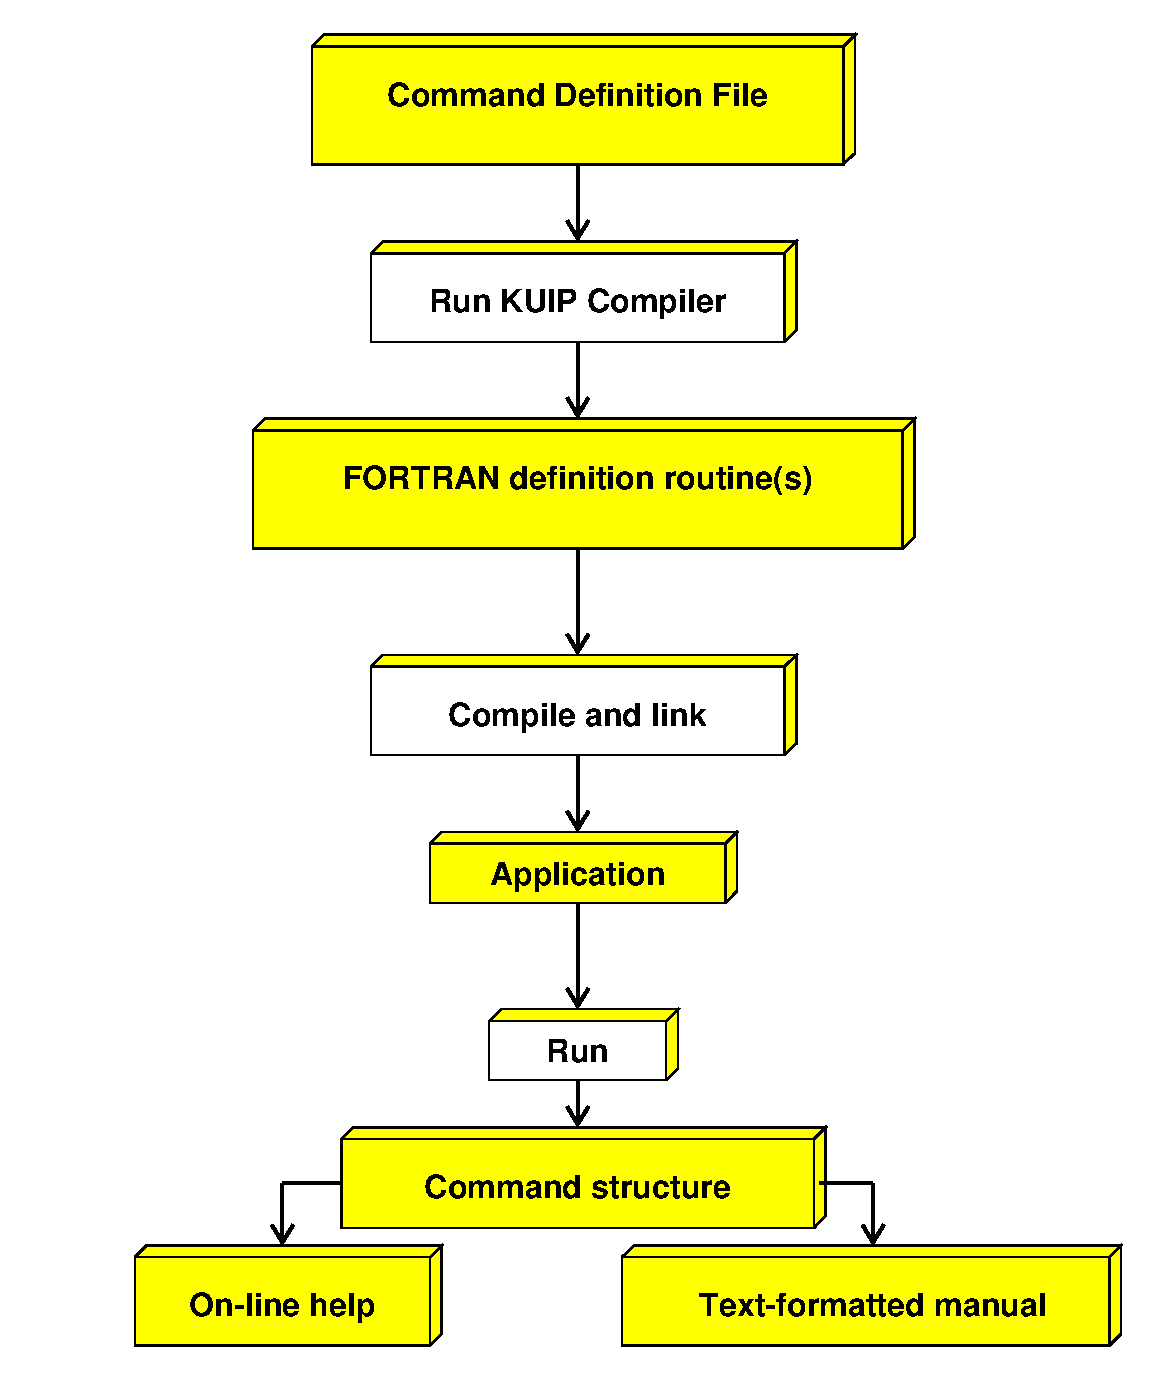
\epsfig{%bbllx=22mm,bblly=30mm,bburx=210mm,bbury=263mm,%
%              file=kuipc.eps,height=12cm}}
\end{center}
\caption{Building an application starting from the \CDF{}.}
\label{FIG8}
\end{figure}

\section{The Command Definition File}

The \CDF{} format is line-oriented.
Completely blank lines are ignored.
An underscore character at the end of a line acts as
continuation symbol, i.e.\ before processing
\index{CDF!continuation lines}
the following line is concatenated to the current line removing the
underscore itself.

Directives
\index{CDF!directives}
starts with a ``\Lit{>}''~character in the first column
immediately followed by the directive name.
Most directives take arguments following on the same line and some
directives expect additional information on separate lines.
\CDF{} argument lines are tokenized according to the rules:
\index{CDF!arguments}
\begin{UL}
\item
Individual arguments must be separated by one or more blanks.
\item
Strings containing blanks must be delimited by single quote characters,
e.g.\ \Lit{'Hello world'}.
\item
Single quote characters inside a string must be duplicated,
e.g.\ \Lit{'N''th value'}.
\item
A single ``\Lit{.}'' is the place-holder for a null argument.
\end{UL}

Names for menus, commands, and parameters
\index{Names}
are case-insensitive and may consists of letters,
digits, minus signs and underscores.
For obvious reasons names containing only digits, starting with a
minus sign, or ending in an underscore should be avoided.
Names may start with a digit.

\section{\CDF{} directives for command definitions\label{basic-CDF}}

The \CDF{} has to define the command tree structure which can contain
three types of elements: 
\begin{UL}

\item
Menus 
\index{menu!definition} 
are the branches of the tree.
Each menu should provide a help text to give general information
about the commands and sub-menus linked to it.

\item
Commands 
\index{command!definition} 
are the terminal leaves of the tree.
The \CDF{} should contain the help text and define the parameters 
(if any).
Each command definition must specify the action routine 
\index{action routine} 
which retrieves the command arguments and performs the intended operations.

\item
Help items \index{help item!definition} are like commands without
action routine. 
Their sole purpose is to provide additional help not related to a
specific command or menu.
Trying to execute a help item is equivalent to asking \Lit{HELP} on that item.

\end{UL}

\condbreak{5\baselineskip}
\begin{Gray}{i}
>* comment
   ...
\end{Gray}
\begin{Gray}{i}
*  comment
\end{Gray}
The \Lit{>*}~directive starts a block comment.
Everything up to the next \CDF{} directive is ignored.
A single line comment is introduced by a ``\Lit{*}''~character in the
first column. 


\begin{Gray}{i}
>NAME  definition-routine
\end{Gray}
The \Lit{>Name} directive defines the name of the routine which
\KUIPC{} will generate, i.e.\ \textsl{definition-routine} must be an acceptable
Fortran \Lit{SUBROUTINE} name.
The application has to \Lit{CALL }\textsl{definition-name} at initialization time
in order to store the command definitions in internal memory.


The first non-comment line in the \CDF{} must always be a \Lit{>Name}
directive. 
The \CDF{} may contain several \Lit{>Name} directives.

\begin{figure}[p]
\begin{XMPtext}{Example for the creation of menus}{
In this example \Lit{CALL KUIPDF} creates the menus \Lit{/KUIP},
\Lit{/KUIP/ALIAS}, \Lit{/KUIP/SET\_SHOW}, and \Lit{/MACRO} and 
\Lit{CALL VECDEF} creates the menu \Lit{/VECTOR}.
}
>Name KUIPDF
>Menu KUIP
>Guidance
      ...
>Menu ALIAS
>Guidance
      ...
>Menu ../SET_SHOW
>Guidance
      ...
>Menu /MACRO
>Guidance
      ...
>Name VECDEF
>Menu VECTOR
>Guidance
      ...
\end{XMPtext}
%\end{figure}
\vspace{-2\baselineskip}
%\begin{figure}[p]
\begin{XMPtext}{Example for the creation of commands}{
In this example the commands \Lit{/KUIP/HELP},
\Lit{/KUIP/ALIAS/CREATE}, and \Lit{/KUIP/ALIAS/DELETE} are created.
}
>Menu /KUIP
>Command HELP
      ...
>Menu ALIAS
>Command CREATE
      ...
>Command DELETE
      ...
\end{XMPtext}
%\end{figure}
\vspace{-2\baselineskip}
%\begin{figure}[p]
\begin{XMPtext}{Example for the creation of a help item}{
This example creates the help item \Lit{/KUIP/FUNCTIONS}.
}
>Menu /KUIP
>Help_item FUNCTIONS
>Guidance
      ...
\end{XMPtext}
\end{figure}

\begin{figure}[p]
\XMPvinput{Example for a guidance text}{xguidance.cdf}{}
\end{figure}

\begin{figure}[p]
\XMPvinput{Resulting HELP menu}{xguidance.hlp}{}
\XMPinput{Formatted output for ``MANUAL MYMENU -LATEX''}{xguidance.tex}{}
\end{figure}

\begin{figure}[p]
\XMPvinput{Example for a user help routine}{xuserhelp.f}{}
\XMPvinput{Terminal output for ``HELP MYMENU''}{xguidance.txt}{}
\end{figure}


\begin{Gray}{i}
>MENU  menu-path
\end{Gray}
Commands are linked into the current menu and the \Lit{>Menu}
directive allows to changes the menu path. 
The \textsl{menu-path} can consist of several components separated
by~``\Lit{/}''. 
The path is relative to the previously valid path unless \textsl{menu-path} starts with a~``\Lit{/}''.
The pseudo-name~``\Lit{..}'' refers to the parent menu.


The names for already existing menus may not be abbreviated.
If a menu is not already existing it is created and should be followed
by a \Lit{>Guidance} directive.

The \Lit{>Name} directive resets the path to the root
menu~``\Lit{/}''. 
Commands and help item should not be linked directly to the root menu.
Therefore the \Lit{>Name} directive should always be a followed by a
\Lit{>Menu} directive. 


\begin{Gray}{i}
>COMMAND  command-name
\end{Gray}
The \Lit{>Command} directive appends a new command to the
current menu.
The \textsl{command-name} must be a bare name without menu path.

The \Lit{>Command} directive must be followed by \Lit{>Guidance} and
\Lit{>Action} directives and can be followed by \Lit{>Parameters} and
\Lit{>User_help} directives in any order.


\begin{Gray}{i}
>HELP_ITEM  help-item-name
\end{Gray}
The \Lit{>Help_item} directive appends a new help item to the
current menu.
The \textsl{help-item-name} must be a bare name without menu path.
The \textsl{help-item-name} cannot contain a menu path.

The \Lit{>Help_item} directive must be followed by a \Lit{>Guidance}
directive and can be followed by a \Lit{>User_help} directive in any order.

\condbreak{2cm}
\begin{Gray}{i}
>GUIDANCE
   text
   ...
\end{Gray}
The \Lit{>Guidance} directive defines the help text attached to the
most recent command tree element created by a \Lit{>Menu},
\Lit{>Command}, or \Lit{>Help\_item} directive.
The help text ends at the next \CDF{} directive.
The formatting rules applied for terminal output and by the 
\Lit{MANUAL} command in \LaTeX{} mode are explained in the example below.


\begin{Gray}{i}
>USER_HELP  user-help-routine
\end{Gray}
The \Lit{>User_help} directive may follow a \Lit{>Command} or
\Lit{>Help_item} directive.
The \textsl{user-help-routine} is called by the \Lit{HELP} command and
allows to add runtime dependent information at the end of the static
\Lit{>Guidance} text. 

The routine has to call \Lit{KUHELP} in order to obtain the 
logical unit where the additional help information should be written to.
The second argument of \Lit{KUHELP} returns the command or help item
name for which \Lit{HELP} was requested.

\begin{Gray}{i}
>PARAMETERS
  mandatory-parameters
+
  optional-parameters
++
  constant-parameters
\end{Gray}
The \Lit{>Parameters} directive heads the parameter definition for a command.
The lines following up to the next directive must be parameter
definitions of the form

\indent\indent\begin{tabular}{llll}
\textsl{parameter-name} & \textsl{prompt-string} & \textsl{parameter-type}
& $[$ \textsl{attribute-list} $]$
\end{tabular}
\vskip\parskip

The underscore continuation has to be used if the complete definition
does not fit onto a single single.
Mandatory and optional parameters are separated by a control line
containing only a ``\Lit{+}''~character in the first column.
If there are only mandatory parameters the ``\Lit{+}''~line is not
required.


Non-positional arguments can be specified
in a command line as \textsl{parameter-name}{\tt=}\textsl{value}.
To allow abbreviations for \textsl{parameter-name} the minimum length has
to be indicated by a ``\Lit{*}''~character, e.g.\
\begin{XMP}
DIR*ECTORY \quad 'Directory path' \quad C
\end{XMP}
defines a parameter \Lit{DIRECTORY} which can be assigned in a command
line as ``\Lit{DIR=}\textsl{value}''.

The \textsl{prompt-string} is used to prompt for missing mandatory
arguments and as labels in the \Motif{} command panel.
Possible \textsl{parameter-type} values are ``\Lit{C}''~for character
strings, ``\Lit{I}''~for integer numbers, and ``\Lit{R}''~for real
numbers.

The \textsl{attribute-list} for mandatory parameters can be empty.
For optional parameters it must specify at least the default attribute:
\begin{XMP} 
D=\textsl{default-value}
\end{XMP}
For mandatory parameters the default value is only used when prompting
for missing arguments and the reply is an empty line.
The default value for optional parameters is passed to the action
routine whenever the argument is missing or given as~``\Lit{!}'' on
the command line.

For all parameter types~\Lit{C}, \Lit{I}, and~\Lit{R} the range
attribute defines a comma-separated list of valid values:
\begin{XMP} 
R=\textsl{value-1},\textsl{value-2},...\textsl{value-n}
\end{XMP}
e.g.\
\begin{XMP} 
PRIME \quad 'Prime number below 10' \quad I \quad R=2,3,5,7
\end{XMP}
For option parameters there is an alternative way to specify the list
of valid values together with an explanation text for each option (see below).
For the numeric parameter types~\Lit{I} and~\Lit{R} the range
attribute can have the form
\begin{XMP} 
R=\textsl{lower-limit}:\textsl{upper-limit}
\end{XMP}
to limit valid values to the interval including the boundaries.
Either the \textsl{lower-limit} or the \textsl{upper-limit} may be
omitted to indicate an unlimited interval in one direction.

Numeric parameters with a limited range are displayed with a slider in
the \Motif{} command panel.
The slider step size for type~``\Lit{R}'' parameters is determined by
the number of digits following the decimal point in the range
definition, e.g.\
\begin{XMP} 
PROB*ABILITY  'Detection probability'  R  D=0.5  R=0:1.00
\end{XMP}
creates a slider for the values 0.00, 0.01, ..., 1.00.
If the range is unlimited or too large the \Lit{Slider} attribute
\begin{XMP} 
SLIDER=\textsl{lower-limit}:\textsl{upper-limit}
\end{XMP}
allows to define a restricted range which affects the slider only.
E.g.\
\begin{XMP} 
EFF*ICIENCY  'Reconstruction efficiency'  R  R=0:1  Slider=0.900:1
\end{XMP}
creates a slider for the values 0.900, 0.901, ..., 1.000.

\begin{figure}[tb]
\XMPvinput{Example for option parameter definitions}{xparameter.cdf}{}
\end{figure}

\begin{figure}[tb]
\XMPvinput{Argument assignments for command ECHO}{xparameter.log}{}
\end{figure}

%\begin{figure}[tb]
%\XMPvinput{Terminal output for ``HELP ECHO''}{xparameter.txt}{}
%\XMPinput{Formatted output for ``MANUAL ECHO -LATEX''}{xparameter.tex}{}
%\end{figure}

The \Lit{Option} attributes defines a parameter to be an option for
which ``\Lit{-}\textsl{value}'' can be used to specify non-positional
option arguments on the command line.
The \Lit{Option} attribute is set implicitly
if \textsl{parameter-name} begins with \Lit{OPTION} or \Lit{CHOPT}.
The ``\Lit{-}''~mechanism requires a range definition including all
valid option values.
The list of option values is defined by lines
\begin{XMP} 
-\textsl{option-value} \quad \textsl{explanation-text}
\end{XMP}
following the option parameter definition itself.
The ``\Lit{-}''~character must be in the first column and is not part
of the option value.
The underscore continuation has to be used if the complete 
\textsl{explanation-text} does not fit onto a single single.
The rules applied for formatting the list of options as a table are
explained in the example. 

A command can contain contain several option parameters as long as the
option values are distinct.
Option values can be specified with the range attribute
if an \textsl{explanation-text} is not required.
Blank is permitted as \textsl{option-value} but cannot be combined with
any other value.
Consequently it should only be used if all option values are mutually
exclusive, and it should be the default value.

The interpretation of a ``\Lit{-}\textsl{value}'' argument as option
is considered only if \textsl{value} consists
exclusively of valid values from a single option parameter.
In some instances ``\Lit{-}\textsl{value}'' is intended be a positional
argument even though it could match an option parameter as well.
It depends then on the definition of the parameter which
should be assigned next whether the argument is actually interpreted
as option ``\textsl{value}''.

If ``\Lit{-}\textsl{value}'' can be interpreted as a negative number
and the next parameter is numeric the option assignment is inhibited.
A character parameter can be given the \Lit{Minus} attribute to
indicate that arguments at its position should never be assign to an
option parameter.

The leading ``\Lit{-}'' is usually stripped off in an option
assignment. 
Only in case the next argument position belongs to the option
parameter itself and ``\Lit{-}'' is one of its option values
it is passed on to the action routine.
In order to avoid confusion due to this position dependence digits and
the minus sign should not be used as option values.


It is often desirable for a command to be able to accept a
variable-length list of values for one of the parameters.
If the command operation is independent for each list item
the \Lit{Loop} attribute can be added to the corresponding parameter
definition.
For a comma-separated argument list the action routine is then called
repeatedly passing it the next list item each time.
E.g.\ with the definition
\condbreak{1cm}
\begin{XMP}
>Command DELETE
>Parameters
LIST  'List of items'  C \quad Loop
\end{XMP}
the command line
\begin{XMP}
DELETE x,y,z
\end{XMP}
is equivalent to
\begin{XMP}
DELETE x ;  DELETE y ;  DELETE z
\end{XMP}
and the action routine only needs to handle a single item.
A ``\Lit{,}'' inside a quoted string or an unbalanced set of
parentheses is not treated as item separator, i.e.\ ``\Lit{'foo,bar'}''
and ``\Lit{xyz(3,4,5)}'' are single items only.

In case the action routine needs access to all list items it can call
\Rind{KUGETL} to retrieve the items one by one.
The \Lit{Vararg} attribute can be given to a list parameter if it is
the last one of the command. 
This allows to use \Rind{KUGETL} also for a blank separated item list,
i.e.\ with the definition
\begin{XMP}
>Command ASSIGN 
>Parameters 
ARRAY  'Array name'  C 
VALUES  'List of values'  C  Vararg
\end{XMP}
both command line forms
\begin{XMP}
ASSIGN  name  foo,bar 
ASSIGN  name  foo  bar
\end{XMP}
can be handled by the same action routine.

In \Motif{} mode the arguments entered in the command panel are usually
treated as a single value, i.e.\ if they contain a blanks they are
implicitly quoted.
In some cases, for example the macro arguments passed in the
\Cind{EXEC} command, this behavior must be inhibited.
The \Lit{Separate} attribute allows to flag the last parameter that
the value entered in the \Motif{} input field should be interpreted as
separate command line tokens.


\condbreak{3\baselineskip}
\begin{Gray}{i}
>ACTION  action-routine
\end{Gray}
The \Lit{>Action} directive must follow a \Lit{>Command} and defines
the routine which should be called after decoding the command line in
order to perform the intended operations.

\begin{figure}[tb]
\XMPvinput{Example for an action routine}{xecho.f}{}
\end{figure}

An action routine does not have arguments.
The command line arguments have to be retrieved 
by calling the suitable \Lit{KUGET}\textsl{x} routine for each parameter
from inside the action routine.

The same action routine can be used for different commands.
The routines \Lit{KUPATH} and \Lit{KUPATL} allow to identify which
command was actually requested.

\if0
\section{Retrieving parameters in action routines}

Action routines are called automatically by \KUIP{} when the corresponding
command is entered. The application programmer, in addition to defining
their names with the \Command{>Action} keyword in the \CDF{}, will have to write
these action routines and to link them together with the rest of its application.

Inside action routines, parameters, as defined with \Command{>Parameters}
in the \CDF{}, have to be retrieved by calling the
\KUGETx{} routines, e.g.:
\Rind[KUGETI]{KUGETI(IPAR)}, \Rind[KUGETR]{KUGETR(RPAR)}, 
\Rind[KUGETC]{KUGETC(CHPAR,NCH)},\ldots for parameters of the
type Integer, Real and Character type parameters respectively.
%
%---------------------------------------------------------------------------
%
\fi
%
%---------------------------------------------------------------------------
%
\section{Browser Concepts and Definitions}
\label{ref:rebrodef}

The high-light of the \KUIPMotif{} interface is a general-purpose object
browser.
Before going into the details of the \CDF{} directives for customizing
the browser we want to introduce the main concepts and the terminology
used.

The browser allows to traverse a hierarchical directory structure of 
objects. Operations on these objects can be chosen from pop-up menus which
depend on the object type (or ``class'').

To incorporate your own application specific objects into the browser
you have to:
\begin{UL}
\item
describe in the \CDF{} (``Command Definition File'') the object types 
(``classes'') and the containers for these objects (``browsables''),
\item
write ``small'' routines to scan through the list of objects, and 
eventually the list of browsables,
\item
describe in the \CDF{} the action menus for classes of objects and browsables.
\end{UL}

\subsection{Classes of Objects}
\label{ref:recldef}

``Classes'' of objects can be any kind of entities handled by an application.

For example:
\begin{UL}
\item
HIGZ pictures and \HBOOK{} data (1d-histograms, 2d-histograms, 
N-tuples, chains and directories) are ``Classes'' defined in
\PAW++{}.
\item
in Geant++  the classes are the data structures: volumes, materials, 
particles, ...
\item
in \KUIPMotif{} the commands themselves have been defined as classes,
as well as the different type of files (read, read-write, executable,
and macros ...).
\end{UL}

Object classes are defined in the \CDF{} with the directive:
\begin{Gray}{i}
>Class  class-name  menu-title  [ big-icon  small-icon ]
\end{Gray}

\begin{figure}[tb]
\begin{PICTf}[.45]{pkmf15}
\begin{DLsf}{}
\item[\quad \CDF{} description (extract) :]
\item
\item
\begin{XMPt}{Example of the ``Class'' directive}\footnotesize

>Class 1d 1d-Histogram big_1d sm_1d
 Plot        .  .  default_action%C
'/Fit...'    .  'Histo/Fit [this]'
'Fit Gauss'  .  'Histo/Fit [this] G'
'Fit Exp'    .  'Histo/Fit [this] E'
'Fit Const'  .  'Histo/Fit [this] P0'
'Fit Linear' .  'Histo/Fit [this] P1'
 /Smooth     .  'Smooth [this]'
'Smooth...'  .  '-Smooth [this]'
 /Copy       .  'Histo/Copy [this]'
 Reset       .  'Histo/Op/Reset [this]'
!Delete      .  'Hio/Hscratch [this]'
+
...
\end{XMPt}
\end{DLsf}
\end{PICTf}
\begin{EnumZB}
\item Icon used to represent the object class ``1d'' (normal size).
\item Action menu (title ``1d-Histogram'') associated to the selected object 
(histogram of class ``1d'' with name/identifier ``10'').
\vspace{-1\baselineskip}
\end{EnumZB}
\caption{Object Classes}
\label{ref:FIGPKMF15}
\end{figure}

E.g.\ The directive ``{\tt >Class 1d '1d-Histogram' big\_1d sm\_1d}'' in the 
\PAW{} \CDF{} is used for 1D histograms : the class name is ``1d'', ``big\_1d''
(normal size) and ``sm\_1d'' (small size) are the icons used by the browser 
for a graphical representation and ``1d-Histogram'' is the title text for
the pop-up menu displayed when object types ``1d'' are selected in the browser
(see figure~\ref{ref:FIGPKMF15}).

\subsection{Browsables}
\label{ref:rebrdef}

All objects are part of container objects constituting the top level directory
(e.g.\ ZEBRA/RZ files.). We will call these containers the ``browsables''.
They are defined with the \CDF{} directive
\begin{Gray}{i}
>Browse  browsable-class  menu-title  scan-objects  [ scan-browsables ]
\end{Gray}

\begin{figure}[tb]
\begin{PICTf}[.5]{pkmf16}
\begin{DLsf}{}
\item[\quad \CDF{} description (extract) :]
\item
\item
\begin{XMPt}{Example of the ``Browse'' directive}\footnotesize

>Browse Commands . kscncmds%C
 List
'Set Default'  .  ' Set/Root /'
...
>Class /Menu Menu big_menu sm_menu
...
>Class Cmd Command big_cmd sm_cmd
...
\end{XMPt}
\end{DLsf}
\end{PICTf}
\begin{EnumZB}
\item The browsable ``Commands'' is selected.
\item Action menu corresponding to this browsable.
\item \OW{} with the list of commands (class ``Cmd'') and menus 
(class ``/Menu'') for the current directory ``/KUIP'' \NbDB{4}.
\vspace{-1\baselineskip}
\end{EnumZB}
\caption{Browsables}
\label{ref:FIGPKMF16}
\end{figure}

For example:
\begin{UL}
\item
in \PAW++{}, a browsable HBOOK (see figure~\ref{ref:FIGPKMF16}) has been
defined, which is a container for any  
kind of \HBOOK{} data (1d/2d histograms and Ntuples).
\item
in \KUIPMotif{}, the browsable ``Files'' contains and displays all files
(read, read-write, executables, and \KUIP{} macros). Another browsable 
``Commands'' has been defined for all the commands and menus defined 
by \KUIP{} and the application.
\end{UL}

For a detailed description of the ``{\tt >Class}'' and
``{\tt >Browse}'' \CDF{} directives see sections~\ref{ref:recdfobj} 
and~\ref{ref:recdfbro}.

\subsection{The ``scan-objects'' routine}

To make the objects belonging to one browsable for a given path (directory)
accessible by the browser, the application has to provide a scanning routine 
which, when called for the first time, returns the first object and
subsequently returns the next object until no more objects are left: this
is what we have called the ``scan-objects'' routine in the \CDF{} directive 
for the browsable definition. The browser passes to this routine the 
identification of the requested subdirectory and expects in return:
\begin{UL}
\item
the object name, e.g.: 
\begin{UL}
\item
for ``{\tt >Browse HBOOK}'' in \PAW++{}: the histogram or Ntuple identifier 
(number).
\item
for ``{\tt >Browse Commands}'' in \KUIPMotif{}: the menu or command name.
\end{UL}
\item
the object class, e.g.: 
\begin{UL}
\item
for ``{\tt >Browse HBOOK}'' in \PAW++{}: ``1d'', ``2d'' or ``Ntuple'' 
(assuming that ``{\tt >Class 1d}'', ``{\tt >Class 2d}'' and 
``{\tt >Class Ntuple}'' have been defined).
\item
for ``{\tt >Browse Commands}'' in \KUIPMotif{}: ``Menu'', ``Cmd'' and ``InvCmd''
(assuming that ``{\tt >Class Menu}'', ``{\tt >Class Cmd}'' and 
``{\tt >Class InvCmd}'' have been defined).
\end{UL}
\item
and eventually a short and a long description text (title) of this object 
(which will be used to display the list of objects in various forms: big icons, 
small icons, text only).
\end{UL}
This ``scan-objects'' routine can be coded in Fortran or in~C. 

\subsection{The ``scan-browsables'' routine}

We have to make a distinction between two kinds of browsables:
\begin{UL}
\item
``single instance'' browsables,
\item
or ``multiple instances'' browsables.
\end{UL}
A ``multiple instances'' browsable gives the possibility to have several
instances of the same browsable. For instance, in \PAW++{}, the browsable
``{\tt >Browse HBOOK}'' which is defined for the ZEBRA/RZ files, acts as a
container for the objects 1d/2d histograms and Ntuples. As it is
possible to have several ZEBRA/RZ files opened at the same time and 
connected to different logical units (LUN), the browsable HBOOK has been
defined as a ``multiple instances'' one. This is done by providing
a second scanning routine from which the name of all the currently connected
instances of a given browsable can be retrieved (e.g.\ for all the ZEBRA/RZ 
files opened and connected to some logical unit  the name is a concatenation
of ``LUN'' and this number, i.e.\ ``LUN8'' for logical unit 8).
This is what we have called the ``scan-browsables'' routine  (optional for a 
``single instance'' browsable) in the \CDF{} directive for the browsable 
definition.

This ``scan-browsables'' routine can be coded in Fortran or in~C.

Note that ``single instance'' browsables are always displayed in the 
browser (as soon as it is created) whereas ``multiple instances''browsables
can be accessed and displayed at run time (e.g.\ in \PAW++{} when a new 
ZEBRA/RZ file is opened).

For a more precise description of the the calling sequence of the 
``scan-objects'' and ``scan-browsables'' routines see section 
\ref{ref:recdfbro}.

\subsection{Directories}

A tree structure of objects can easily be achieved by defining a special class
for subdirectories of a browsable. The corresponding \CDF{} directive 
is the same 
as for simple object classes, ``{\tt >Class}'', except that there must a 
``{\tt /}'' in front of the class name.

For example:
\begin{UL}
\item
in \PAW++{}, ZEBRA/RZ directories (browsable ``HBOOK'') are ``directories''
classes of objects: 
\begin{XMPt} {}
       >Class /dir Directory big\_dir sm\_dir
\end{XMPt}
Ntuple chains (in the ``Chains'' browsable) are also defined as a ``directory'' 
class of objects:
\begin{XMPt} {}
       >Class /chain Chain big\_chain sm\_chain
\end{XMPt}
\item
in \KUIPMotif{} the menus (in the ``Commands'' browsable) are defined as 
a ``directory'' class of objects:
\begin{XMPt} {}
       >Class /Menu Menu big\_menu sm\_menu
\end{XMPt}
This is also true for directories of files (in the ``File'' browsable):
\begin{XMPt} {}
       >Class /DirFile Directory big\_menu sm\_menu
\end{XMPt}
\end{UL}

This ``special'' class of objects obeys to certain rules:
\begin{UL}
\item
The first item in the action menu is always ``List'' and means ``switch into 
this subdirectory''. Selecting this item (automatically performed with 
a <double click> with the left button) has the effect to update
the content of the \OW{} with the list of objects contained
into the new subdirectory.
\item
The entry ``Path:'' (Fig. \ref{ref:FIGPKMF16}, 
\NbDB{4}) is automatically updated
with the new directory path, which is formed by concatenating the previous
path, a ``{\tt /}'', and the name of the directory object selected.
Going upwards in the directory hierarchy is done by selecting a
substring of the current path displayed in this text entry. Clicking
a second time on the same path segment performs the directory change
and updates the \OW{} in the same way as selecting the ``List'' 
menu entry for a directory object.
\end{UL}

\subsection{Action menus}

For each class of objects it is possible to define two menus which describe 
possible actions if an object of this class is selected:
\begin{UL}
\item[(1)]
either in the browser \OW{},
\item[(2)]
or identified inside a HIGZ \GW{} (if any).
\end{UL}

\condbreak{3\baselineskip}
For each browsable it is possible to define:
\begin{UL}
\item[(3)]
one menu which describes possible 
actions if this browsable is selected (\BW{}), 
\item[(4)]
for ``multiple instances'' browsables, a second menu which describes 
the actions required to connect or de-connect one instance of this 
browsable at run time (menu ``File'' in the \MB{}).
\end{UL}

Menus (1), (2) and (3) pop up when pressing the right mouse button 
in the corresponding window, and the
selected action is performed when the button is released. A <double click>
with the left mouse button on one specific object or on one specific 
browsable always executes the first menu item. Menu (4) is accessed by 
selecting the entry ``File'' in the \MB{} menu-bar.

Object and browsable specific action menus are derived from sequences of action 
definitions written in the \CDF{} and following the {\tt >Class} or 
{\tt >Browse} directive (Fig. \ref{ref:FIGPKMF15} and \ref{ref:FIGPKMF16}). 
For a precise description of the syntax and behavior 
of the \CDF{} directives for action menus see section \ref{ref:recdfacm}.


\section{\CDF{} directives for \KUIPMotif{}\label{Motif-CDF}}

\label{ref:recdf}

We will describe in this section the new \CDF{} (Command Definition File)
directives which have been introduced in \KUIPMotif{}. Please note that
these new directives have to be used only to take advantage of the MOTIF
style and to include your application specific objects into the interface
(and especially into the browser(s)). BUT one must be aware that IT IS 
POSSIBLE to get a \Motif{} interface for any \KUIP{} based application 
WITHOUT modifying the \CDF{}, but only modifying very slightly the 
application main program in order to give control to the ``\Motif{} main loop'' 
(i.e.\ call KUWHAM instead of KUWHAT or KUWHAG).

In all the directives we will describe the square brackets (``[]'') mean
that the corresponding entity is optional: either some default value
is automatically provided if it is missing (e.g.\ for titles), or the
entity is not necessary requested. If such an optional entity happens
to be in the middle of the directive (not at the end) then it has
to be replaced by a ``.'' if no real value is given.

We advice users who want to take advantage of the \Motif{} style to compile 
their \CDF{}s into C~code (instead of Fortran): this is automatically 
performed by the \KUIPC{} compiler when giving the extension ``\Lit{.c}'' to the 
output file which is produced.

N.B. It is preferable to separate the directives for the usual command mode
interface and the directives specific to the \Motif{} style (objects, browsables
and action menus definitions) into different \CDF{}s. Then it will be easy
and possible to make the same application work on a dumb terminal (offering 
only the \KUIP{} command mode interface) or on a \Motif{} workstation, with only 
very few differences in the application main program. 

\subsection{For Classes of Objects}
\label{ref:recdfobj}

As we have already seen (section \ref{ref:recldef}), classes of objects 
are defined in the \CDF{} with the directive
\begin{Gray}{i}
>Class  class-name  menu-title  [ big-icon  small-icon ]
\end{Gray}
for example,
\begin{XMP}
>Class ExFile 'Executable File' big_fx sm_fx
\end{XMP}

The ``menu-title'' should be a short explanation concerning the class (or type)
of object and is used as a title text for the action menu which is displayed
when one object of this class is selected (either in the browser, or in the
\GW{} if any). If no title is given the ``class-name'' is used 
instead. 

``big-icon'' and ``small-icon'' are the names for the icons representing 
graphically this class of object inside the browser. Default icons are
provided if these values are missing, but then the same iconic representation
will be used for all object classes. It is a lot better to have a different
representation for each object class. To create a new icon bitmap you can use
the X11 standard bitmap editor. The icons definitions in the \CDF{} follow
the directive {\tt >Icon\_bitmaps} (see \ref{ref:rebmdef}).


\subsection{For Browsables}
\label{ref:recdfbro}

As we have seen in section \ref{ref:rebrdef}, browsables are defined with the 
\CDF{} directive
\begin{Gray}{i}
>Browse  browsable-class  menu-title  scan-objects  [ scan-browsables ]
\end{Gray}
for example,
\begin{XMP}
>Browse Macro . kmbmac%C kmbmdi%C
\end{XMP}

The ``menu-title'' should be a short explanation on the browsable itself
and is used as a title text for the action menu which is displayed
in the browser ``FileList'' window when this browsable is selected. If a 
``.'' is put instead, then the browsable-class becomes by default the 
menu-title.

\subsubsection{The ``scan-objects'' Routine}
\label{ref:recdfsco}

The ``scan-objects'' routine can be written in Fortran or in~C. 
The browser passes to this routine the identification of the requested 
subdirectory (path) and expects in return: the object name, the class 
name, and eventually a short and a long description text (title) of this 
object. In both cases (Fortran or~C) the calling sequence is predefined. 

In Fortran the calling sequence of the ``scan-objects'' routine 
is the following:
\condbreak{3cm}
\begin{XMPt}{scan-objects routine (in Fortran)}\footnotesize
      SUBROUTINE SCNOBJ(BRNAME,BRCLAS,BRPATH,OBNAME,OBCLAS,STEXT,LTEXT)
      CHARACTER*(*) BRNAME,BRCLAS,BRPATH,OBNAME,OBCLAS,STEXT,LTEXT
*
*            Browser interface to return next object
*
*            Input Parameters  :
*
*                      BRNAME  : browsable name (displayed in the browser)
*                      BRCLAS  : browsable class name (from the ``>Browse'' directive)
*                      BRPATH  : current directory path
*
*            Input / Output    :
*
*                      OBNAME  : object name or identifier
*                                ' ' the first time, previous object otherwise
*
*            Output Parameters :
*
*                      OBCLASS : class name                
*                      STEXT   : short text description of the object
*                      LTEXT   : long text description of the object
*
*     ...
*     IF(OBNAME.EQ.' ') THEN
*        Initialize the scan-objects routine        
*     ENDIF
*     ...
*
      OBCLASS = ...
      STEXT = ...
      LTEXT = ...
*
      END
\end{XMPt}

\condbreak{4cm}

In C the calling sequence is:
\begin{XMPt} {scan-objects routine (in C)}
char **scnobj( brobj_name, brcls_name, bpath, n )
     char *brobj_name;  /* browsable name (displayed in the browser) */
     char *brcls_name;  /* browsable class (from the ``>Browse'' directive) */
     char *bpath;       /* current directory path */
     int n;             /* object position (0 the first time) */
\{
  static char     *obj_desc[4];

    ...
    if (n == 0) \{
       /* Initialize the scan-objects routine */
    \}
    ...

    return obj_desc;   /* obj_desc[0] --> object name or identifier
                          obj_desc[1] --> class name
                          obj_desc[2] --> short text description of the object
                          obj_desc[3] --> long text description of the object
                        */
\}
\end{XMPt}

The browsable name and class-name are identical for ``single instance'' 
browsables. They can be different for ``multiple instances'' browsables.
e.g.\ for ``{\tt >Browse HBOOK}'' in \PAW++{}: the browsable class is ``HBOOK'' 
and the browsable name is ``LUN8'' for a ZEBRA/RZ file connected to logical 
unit 8.

The selected object name (or identifier) and its corresponding long text 
description are printed at the very bottom line of the browser
(\NbDB{6} in Fig.\ref{ref:FIGPKMF9}).

\subsubsection{The ``scan-browsables'' Routine}
\label{ref:recdfscb}

The ``scan-browsables'' routine (optional for ``single instance'' browsables 
but required for ``multiple instances'' ones) can be written in Fortran or 
in~C.  The browser passes to this routine the browsable class-name (e.g.\ 
in \PAW++{}, ``\Lit{HBOOK}'' for ZEBRA/RZ files) and expects in return: the browsable 
name (e.g.\  ``\Lit{LUN8}'' for a ZEBRA/RZ file connected to logical unit~8)
and eventually a string with the description of a predefined set of 
variables concerning this browsable. These variables are used as ``key-words''
in the actions menus connected to the browsables or the classes of objects. 
Some of these variables are fixed by \KUIPMotif{} itself:
\begin{UL}
\item
the variable ``file'' is used to fill the corresponding label (``File:'') 
at the bottom of the browser. 
\item
``root'' is used for setting the path of the top level directory 
(e.g.\ ``\Lit{//LUN8}''),
\end{UL}
The `scan-browsables'' routine for a ``single instance'' browsable can be 
defined just for setting this ``description string'' with the required
key-words.

\condbreak{4cm}

In Fortran the calling sequence of the ``scan-browsables'' routine 
is the following:
\begin{XMPt}{scan-browsables routine (in Fortran)}\footnotesize
      SUBROUTINE SCNBRO(BRCLAS,BRNAME,VARSET)
      CHARACTER*(*) BRCLAS,BRNAME,VARSET
*
*            Browser interface to return next browsable instance
*
*            Input Parameters  :
*
*                      BRCLAS  : browsable class name (from the ``>Browse'' directive)
*
*            Input / Output    :
*
*                      BRNAME  : browsable name (displayed in the browser)
*                                ' ' the first time.
*
*            Output Parameters :
*
*                      VARSET  : set of variables for this browsable.
*
*     First call to this routine 
      IF(BRNAME.EQ.' ') ...
*
      ... 
\condbreak{7\baselineskip}\vspace{-\baselineskip}
      BRNAME = ...
      VARSET='root= ... file= ... ...=...'
      ...
*
      END
\end{XMPt}
E.g.\ in \PAW++{}, for ``{\tt >Browse HBOOK}'' and the browsable ``LUN8'' (ZEBRA/RZ
file connected on logical unit 8) the routine SCNBRO will return something
like:
\begin{XMP}
VARSET = root=//LUN8 file='/user/paw/demo/hrztest.dat'  unit=8
\end{XMP}
In this example ``unit'' is a key-word specific to the browsable HBOOK that 
can be used later on in the action menu definition (e.g.\ ``Close [unit]'').
(See next section \ref{ref:recdfacm} for a complete description of the 
``action menu definition'').

\condbreak{4cm}
In C the calling sequence is the following:
\begin{XMPt} {scan-browsables routine (in C)}
char **scnbro( class_name, first )
     char *class_name;
     int first;
\{
    static char *path_desc[2];

    ...
    if (first) {
       /* First call to this routine */
    }
    ...

    return path_desc;  /* path_desc[0] --> browsable name
                          path_desc[1] --> set of variables for this browsable
                        */
\}
\end{XMPt}

\subsection{For Actions Menus}
\label{ref:recdfacm}

Both the ``{\tt >Class}'' and ``{\tt >Browse}'' directives can be followed 
by sequences of action definitions which obey to the following syntax:
\begin{Gray}{i}
menu-text  [ special-flags ]  [ action-string ]  [ action-routine ]
\end{Gray}
N.B. the components which are missing, when optional (enclosed with ``[]'' 
in the syntax description above), must be replaced by a ``.'' if they are
not the last ones.

The ``menu-text'' is the text that will appear in the pop-up menu. It should
be short but meaningful. ``/'' and ``!'', when they are the very first 
character of this menu-text have special meanings:
\begin{UL}
\item
a ``/'' means that the menu item has to be preceded by a separator,
\item
a ``!'' means that the browser has to be updated when the action is
performed (because the ``objects window'' may have changed).
\end{UL}

The entity ``special-flags'' is not used at the moment and has to be
replaced by a ``.''.

The action can be specified as a string of commands (``{\tt action-string}'')
which should be executed and/or a user-written and application specific 
routine (``{\tt action-routine}'') which should be called. 

In both cases (``{\tt >Class}'' and ``{\tt >Browse}'') two sets of menus 
can coexist and are separated by a blank line starting with the 
character ``+''. The first menu always applies to objects/browsables 
which are identified in the browser. In most cases the
menu pops up when pressing the right mouse button and the selected
action is performed when the button is released.

For the ``{\tt >Class}'' directive the second menu applies to objects which 
are identified in the HIGZ \GW{} if any. (E.g.\ in \PAW++{}, 
``{\tt >Class 1d}'' and ``{\tt >Class 2d}'' histograms can be 
identified either in the browser or in the graphics window: two sets of
menu are then defined in the \CDF{}). 

For the ``{\tt >Browse}'' directive a second menu can be defined to fill 
the ``File'' menu-bar entry in the browser with the list of commands to 
connect or de-connect one instance of a ``multiple instances'' browsable 
(e.g.\ in \PAW++{} open or close a ZEBRA/RZ file containing \HBOOK{} data). 

Only one of the two menu sets can be defined in both cases.

N.B. For graphical object identification inside the graphics window 
please refer to the description of the two HIGZ routines \IGPID{} and
\IGOBJ{} in the HIGZ manual \cite{bib-HIGZ}.

\subsubsection{Action-string (String of Commands)}

When the action is specified as a string of commands,
constructs of the form ``{\tt [}{\em var}{\tt ]}'' can insert
identifications of the selected object in the command string:
\begin{UL}
\item
{\tt [this]} is replaced by the object name, e.g.\ in \PAW++{}: histogram ``10''.
\item
{\tt [that]} is replaced by the short description text returned by the
scanning routine and can thus be used as an alias name.
\item
{\tt [name]} is replaced by the name of the browsable,
e.g.\ in \PAW++{}, ``{\tt LUN8}'' for an ZEBRA/RZ file opened on unit~8.
\item
{\tt [root]} is replaced by the path of the top level directory,
e.g.\ in \PAW++{}, ``{\tt //LUN8}''.
\item
{\tt [path]} is replaced by the complete path to the directory in which the
object is contained, e.g.\ in \PAW++{}, ``{\tt //LUN8/MYDIR}''.
Initially, {\tt [path]} is set to {\tt [root]}.
\end{UL}

As we have seen in the previous section (\ref{ref:recdfscb}) the replacement
values for {\tt [name]}, {\tt [root]} and, eventually, additional 
variables specific to the application (e.g.\ {\tt [unit]} in \PAW++{} for
the browsable HBOOK) have to be returned by the application specific
``scan-browsables'' routine. For single instance
browsables, when this routine (optional) is not defined, {\tt [name]} is 
substituted by the class name and the field {\em menu-title} of the 
{\tt >Browse} directive is used as the definition of {\tt [root]}.


\subsubsection{Action-routine}

If the action corresponding to some menu-text is specified as an 
action-routine, it can be coded either in Fortran or in~C. 
Fortran is the default, for C~coding the 
two characters ``\Lit{\%C}'' must be appended at the end of the routine name. 

The predefined calling sequence of the action routine in Fortran depends on 
which entity the action menu applies:
\begin{UL}
\item[]
Case 1: menu defined for browsables (in the \BW{}).
\begin{XMPt} {Action-routine Skeleton (Fortran)}
      SUBROUTINE ACTION(BRNAME,BRCLAS,BRPATH)
      CHARACTER*(*) BRNAME,BRCLAS,BRPATH
*
*     Write application code ... 
*
      END
\end{XMPt}
\condbreak{3\baselineskip}
\item[]
Case 2: entry in the menu ``File'' (to connect a new browsable instance).
\begin{XMPt} {Action-routine Skeleton (Fortran)}
      SUBROUTINE ACTION(BRCLAS)
      CHARACTER*(*) BRCLAS
*
*     Write application code ...
*
      END
\end{XMPt}
\item[]
Case 3: menu defined for objects which are identified in the browser \OW{}.
\begin{XMPt} {Action-routine Skeleton (Fortran)}
      SUBROUTINE ACTION(BRNAME,BRCLAS,BRPATH,OBNAME,OBCLAS,STEXT,LTEXT)
      CHARACTER*(*) BRNAME,BRCLAS,BRPATH,OBNAME,OBCLAS,STEXT,LTEXT
*
*     Write application code ...
*
      END
\end{XMPt}
\item[]
Case 4: menu defined for the objects identified in the graphics window.
\begin{XMPt} {Action-routine Skeleton (Fortran)}
      SUBROUTINE ACTION(OBNAME,OBCLAS)
      CHARACTER*(*) OBNAME,OBCLAS
*
*     Write application code ...
*
      END
\end{XMPt}
\end{UL}
In all cases the meaning of the input parameters is exactly the same as for
the ``scan-objects'' routine (section \ref{ref:recdfsco}):
\begin{XMP}
      BRNAME  : browsable name (displayed in the browser)
      BRCLAS  : browsable class name (from the ``>Browse'' directive)
      BRPATH  : current directory path
      OBNAME  : object name or identifier
      OBCLASS : class name
      STEXT   : short text description of the object
      LTEXT   : long text description of the object
\end{XMP}

In C the calling sequence is always the same, and is predefined as follows:
\begin{XMPt} {Action-routine Skeleton (C)}
#include <stdio.h>
#include <Xm/Xm.h>

typedef enum \{
  BRACT_OPEN = 0,
  BRACT_ROOT = 1,\condbreak{3\baselineskip}
  BRACT_CONT = 2,
  BRACT_GRAF = 3
\} BrActTag;

typedef struct _BrClientdata \{
  BrActTag    tag;
  char       *brobj;
  char       *brcls;
  char       *path;
  char       *kmobj;
  char       *kmcls;
  char       *stext;
  char       *ltext;
  char       *mtext;
\} BrClientdata;

void action-routine (w, client_data, cbs)
   Widget w;
   BrClientdata *client_data;
   XmAnyCallbackStruct *cbs;
\{
   /* Write application code ... */
\}
\end{XMPt}
N.B. This is the ``usual'' syntax for a ``call-back'' routine with \Motif{}.

The input parameter "client\_data" (structure BrClientdata) contains all 
the information which may be required according to which entity the action 
menu applies. 

The description of the structure BrClientdata follows:
\begin{XMP}
  tag   ---> BRACT_OPEN (menu ``File'' in the browser) , 
             or BRACT_ROOT (``Browse'' menu), 
             or BRACT_CONT (``Class'' menu in the browser),
             or BRACT_GRAF (``Class'' menu in the graphics window).
  brobj ---> browsable name (displayed in the browser)
  brcls ---> browsable class name (from the ``>Browse'' directive)
  path  ---> current directory path
  kmobj ---> object name or identifier
  kmcls ---> class name
  stext ---> short text description of the object
  ltext ---> long text description of the object
  mtext ---> menu text
\end{XMP}

\subsubsection{Example}

The following is an example of the action menus definition for the object
class ``1d'' in \PAW++{} (1-dimensional histogram):

\begin{XMPt} {Example of action menus definition}
>Class 1d 1d-Histogram big_1d sm_1d
 Plot                           .  . default_action%C
'/Fit...'                       .  'Histo/Fit [this]'
'Fit Gauss'                     .  'Histo/Fit [this] G'
'Fit Exp'                       .  'Histo/Fit [this] E'
...
'Smooth...'                     .  '-Smooth [this]'
 /Copy                          .  'Histo/Copy [this]'
 Reset                          .  'Histo/Op/Reset [this]'
!Delete                         .  'Histo/Hio/Hscratch [this]'
+
'Fit...'                        .  'Histo/Fit [this]'        default_G_action%C
'Fit Gauss'                     .  'Histo/Fit [this] G'      default_G_action%C
...
'Filled Lego'                   .  'Histo/Plot [this] LEGO1' default_G_action%C
'Default'                       .  'Histo/Plot [this]'       default_G_action%C
\end{XMPt}
As the object ``1d'' can be identified both in the browser (for the browsable 
HBOOK) and in the HIGZ \GW{} two sets of menus are defined separated
with a blank line starting with ``+''. 

By default the commands in the action string are executed immediately,
provided that all mandatory arguments are present. If any mandatory 
argument is missing the corresponding \CAP{} comes up 
where they can be filled in. This default behavior can be modified in 
several ways:
\begin{UL}
\item
At run-time, pressing the {\tt CTRL}-key when popping up the menu forces the
command panel even if all mandatory arguments are specified.
\item
Putting a ``{\tt -}'' in front of the command name (``{\tt action-string}'' 
definition in the \CDF{}) forces the \CAP{} as well.
\item
Putting a ``{\tt +}'' in front of the command name never produces a
command panel, independently of the state of the {\tt CTRL}-key.
\end{UL}

The calling sequence of the action routines ``default\_action''
 and ``default\_G\_action'' (coded in ANSI C) is the following:

\begin{XMPt} {action-routine calling sequence (Example)}
void default_action(Widget w, BrClientdata *client_data,
                    XmAnyCallbackStruct *cbs)
\{
   /* Write application code ... */
\}

void default_G_action(Widget w, BrClientdata *client_data,
                      XmAnyCallbackStruct *cbs)
\{
   /* Write application code ... */
\}
\end{XMPt}

\subsection{For Graphical Objects Identification}
\label{ref:regraph1}

A pop-up menu of actions can easily be defined in the \CDF{} for the objects
that are graphically ``pick-able'' in the \GW{} (if any) 
with the HIGZ routine \IGOBJ{} \cite{bib-HIGZ}.

The only thing to do is to define a ``Class'' for this object, and 
define for this class the second action menu which applies to the graphics
window. If this type of object does not appear in the browser it is
not necessary to define for this class neither the first menu nor the icon
representation. 

E.g.\ in \PAW++{} such classes exist for the x- and y-axis:

\begin{XMPt} {X- and Y- axis Definition in PAW++ \CDF{}}
>Class x-axis 'X Axis'
+
'Logarithmic'                          . 'Option LOGX ; Histo/plot [this]'
'Linear'                               . 'Option LINX ; Histo/plot [this]'
'/Sort in alphabetical order'          . 'Sort [this] AY ; Histo/plot [this]'
...
'Character Font...'                    . '-Set VFON ; Histo/plot [this]'
'Axis Color...'                        . '-Set XCOL ; Histo/plot [this]'

>Class y-axis 'Y Axis'
+
'Logarithmic'                          . 'Option LOGY ; Histo/plot [this]'
'Linear'                               . 'Option LINY ; Histo/plot [this]'
'/Sort in alphabetical order'          . 'Sort [this] AY ; Histo/plot [this]'
...
'Character Font...'                    . '-Set VFON ; Histo/plot [this]'
'Axis Color...'                        . '-Set YCOL ; Histo/plot [this]'
\end{XMPt}


\subsection{For Customizing Your Application}
\label{ref:recustomize}

Some \CDF{} directives have been defined in order to facilitate and perform the 
customization of any application as well as possible. For instance the 
default size and positions of the windows opened by \KUIPMotif{} (``Executive'', 
``Browser'' and eventually the ``Graphics'' window) may not be 
suitable for your own application. It is also a lot better to use your own
iconic representation for the application defined objects rather than
the default ones. You may also want to add your own buttons or menu items
in the \EW{} (KXTERM).

On another hand, if the interface offered by \KUIPMotif{} is not sufficient 
for your application and if you want to get involved in \Motif{} programming 
you are free to do so. This is what is done for example in \PAW++{} for the 
``Histogram Style Panel'' and the ``Ntuple Viewer'' which are 
written directly with \Motif{}.

All the directives which are described in this section (apart from the
``{\tt >Graphics}'' one if you want a HIGZ graphics window) are not at all
mandatory and have to be used only if you want to give a more 
``professional'' look to your own application. It can also make your life
easier if you really want to play with \Motif{} !


\subsubsection{Graphical Window Managed by HIGZ}
\label{ref:regraph2}

\KUIPMotif{} can be interfaced to the X11 version of the HIGZ graphics package
for an application which requires high level graphics.
In order for the two packages to cooperate properly, applications
using HIGZ have to add the CDF directive
\begin{Gray}{i}
>Graphics
\end{Gray}
at the beginning of the \CDF{} and call {\tt KUINIM} before calling {\tt IGINIT}.
 
HIGZ allows one to store the name and the class for
every displayed object by calling the routine \Lit{IGPID}.
From this information \KUIPMotif{} can identify the object at the mouse
pointer position and pop up the second set of action menus defined with the
\Lit{>Class} directive (see section \ref{ref:regraph2}). This mechanism is
extensively used in the Motif versions of GEANT (Geant++) and PAW (Paw++).
 
 
\subsubsection{Buttons and Menu(s) Definition}

An application can create its own buttons and pull-down menus either in the
\EW{} (KXTERM) or the main browser window using the \CDF{} directive
\begin{Gray}{i}
>Button menu-title button-label action-routine mnemonic
        accelerator accelerator-text [flag]
\end{Gray}
 
\begin{UL}
\item \textem{menu-title}
    is the title of the pull-down menu where the button has to be put.
    If it does not exist, a new pull-down menu with this title is created.
\item \textem{button-label} is the text label of the menu entry to be created.
\item \textem{action-routine} is the associated action automatically called
    for a ``Button Press'' event.
    It can be a string of commands or a routine coded in C or in Fortran~77.
    (If the routine is in~C the name has to be ended with
    ``\Lit{%C}'' in the CDF declaration).
\item \textem{mnemonic} is a mnemonic definition for the label.
\item \textem{accelerator} and \textem{accelerator-text}
     are accelerator definition for the label.
\item if \textem{flag} = ``\Lit{BR}'' menus/buttons are created in the 
main browser
     (instead of the executive window, by default).
\end{UL}
 
 
\if0
An application can create new buttons and pull-down menus in the
\EW{} (KXTERM) using the \CDF{} directive
\SKUIP[Button] {>Button} { call-back-routine menu-title [/]button-label [mnemo.] [accel.]} 
The calling sequence of the call-back routine (written in C) is:
\begin{XMP}
void call_back_routine(argv, argc)
     char **argv;
     int argc;
\end{XMP}

The ``menu-title'' is the title of the pull-down menu entry in the \EW{}
menu-bar. It can be an already existing entry ("File", "Edit", 
"View" or "Option") in which the new button will be added, or it can 
be a completely new one (for defining a new pull-down menu).

The ``button-label'' is the label corresponding to the new button to
be defined. If it starts with a ``/'' it means that the button must
be preceded in the menu by a ``separator''. 

The two optional entities ``mnemonic'' and ``accelerator'' have to be
given to define respectively the button mnemonic key (which activates
the button if it is pressed while the button is visible)  and the accelerator 
(key that may be used to select the button). 

\fi

\subsubsection{Icon Bitmaps Definition}
\label{ref:rebmdef}

The \CDF{} directive
\begin{Gray}{i}
>Icon_bitmap
\end{Gray}
is followed by the bitmaps definitions for all the icons which will be used
in the browser for the different classes of objects.
 
The application can define its own icons to represent objects in the browser.
Each class definition allows one to specify the names of ``big'' and
``small'' icons which are looked up in the table of available icon bitmaps.
The same icon is used for both sizes  only one of them is defined.
If none is defined then a default icon is used.
The {\tt >Class} directive refers to icons by name, e.g.\ ``\Lit{sm\_myicon}''.
 
To create a new icon bitmap one can use the X11 standard bitmap
editor, e.g., to get a $20\times20$ pixel icon called
``\Lit{small_1d}'' one can type: \Ucom{bitmap small\_1d.bm 20x20}.
Then the output file \Lit{small_1d.bm} containing
``\Lit{#define small_1d_width 20} ...'' simply needs to be inserted into
the CDF following the directive \Lit{>Icon_bitmaps}, for instance,
\begin{XMP}
>Icon_bitmaps
#define sm_myicon_width 18
#define sm_myicon_height 22
static char sm_myicon_bits[] = \lcb
   0xff, 0xff, 0x03, 0x01, 0x00, 0x02, 0x81, 0x07, ...
   0x21, 0x10, 0x02, 0x21, 0x10, 0x02, 0x21, 0x10, ...
   0x41, 0x08, 0x02, 0x81, 0x04, 0x02, 0x01, 0x03, ...
   0x81, 0x04, 0x02, 0x41, 0x08, 0x02, 0x41, 0x08, ...
   0x21, 0x10, 0x02, 0x21, 0x10, 0x02, 0x41, 0x08, ...
   0x01, 0x00, 0x02, 0xff, 0xff, 0x03\rcb;
#define big_myicon_width 36
   ...
\end{XMP}
\Lit{KUIPC} compiles the bitmaps into the application, i.e.,
there is no need for separate bitmap files at run-time.
Alternatively bitmap files can be specified as resources in
\Lit{.Xdefaults} overriding CDF bitmaps of the same name.
 
\subsubsection{Help Definition}
\label{ref:rehlpdef}

Many ``Help'' buttons or menu items are automatically created by \KUIPMotif{}
but for some of them the information required depends directly from the
application. This information can be written in the \CDF{} following the
``{\tt Help\_item}'' directive with predefined key-words.
 
\condbreak{3\baselineskip}
\begin{Gray}{i}
>Help_item  HELP_EXE
\end{Gray}
This help concerns the application itself. It can be accessed in the ``Help''
menu of the \EW{} (KXTERM) or the ``Browser Window'', for
the menu entry ``On application-name'' (e.g.\ ``On \PAW++{}'').
 
\begin{Gray}{i}
>Help_item  HELP_EXE_RESOURCES
\end{Gray}
This help concerns the X Resources specific to the application. It can be
accessed in the ``Help'' menu of the \EW{} or the
`Browser Window'', for the menu entry ``On application-name Resources''
(e.g.\ ``On \PAW++{} Resources'').
 
\begin{Gray}{i}
>Help_item  HELP_[brclass]
\end{Gray}
It is possible to define such a ``help'' for each browsable definition,
by replacing ``[brclass]'' with the browsable-class name.
The ``help'' for a specific browsable can be accessed by selecting the
last entry of the pop-up menu which is displayed when pressing the <mouse
button 3> (the last entry of this menu is always ``Help'').
 
 
It is also possible to use the \CDF{} directive ``{\tt >Help\_item}'' for
your application specific ``Help'' buttons or menus, in the case
you have been involved in direct \Motif{} programming. In that case
you can use the \KUIPMotif{} user callable routine ``km\_do\_help'' for
the call-back associated to your ``help'' button, in the following
way:
 
\begin{XMP}
    extern void km_do_help();
 
    char *help_string = ...  /* key-word for ``Help_item'' */
 
    XtAddCallback (helpB1,XmNactivateCallback,
                   (XtCallbackProc)km_do_help,(XtPointer)help_string);
\end{XMP}
 
This routine simply executes the \KUIP{} command: ``/KUIP/HELP help\_string''
where ``help\_string'' is the key-word which follows a ``{\tt >Help\_item}''
directive.
 
\subsubsection{Hooks}
\label{ref:rehooks}

If one wants to get involved in Motif programming one is free to do so.
KUIP/Motif provides hooks that an application can link its own Motif
code in.
 
The \CDF{} directive
\begin{Gray}{i}
>Motif_customize  fall-back-routine  widget-routine
\end{Gray}
defines two routines
which are called at the initialization phase.
\begin{UL}
\item
the first routine (``fall-back-routine'') has to return the application
specific fall-back resources. These user fall-backs are appended
at the end of \KUIP{} fall-backs (which can then be overwritten).
The return value must be a pointer to a NULL-terminated array of 
resource specification
strings to be used if the application class resource file cannot be opened
or read. This is also a good way to change the default resource values
without having to edit an application class resource file.
\hfill\break
The routine (C coded) has no parameter and the calling sequence is:
\begin{XMP}
static String fall_backs[] = \{
 ...
 NULL
\};
String *fall_back_routine ()
\{
   return fall_backs;
\}
\end{XMP}
 
E.g.\ in \PAW++{}, this routine is called get\_paw\_fallbacks:
\begin{XMPt} {Example of a ``fall-back-routine'' (get\_paw\_fallbacks)}
static String paw\_fallbacks[] = \{
 "Paw++*kxtermGeometry:                  650x450+0+0",
 "Paw++*kuipGraphics_shell.geometry:     600x600-0+0",
 "Paw++*kuipBrowser_shell.geometry:      +0+485",
 "Paw++*histoStyle_shell.geometry:       +670+635",\condbreak{4\baselineskip}
 "Paw++*iconForeground:                  grey40",
 ...
 NULL
\};
String *get\_paw\_fallbacks ()
\{
   return paw\_fallbacks;
\}
\end{XMPt}
For a more precise description of the most important \KUIPMotif{} X resources
see section \ref{ref:rekmres}.
\item
the second routine (``widget-routine'') is called by \KUIP{} after creating
every top level widget (\EW{}, any browser instance, graphics window)
in order to customize these widgets: e.g.\ to define and set your own
pixmaps for the iconic state of each window, to change the titles, etc.
\hfill\break
The routine (C coded) has two input parameters: the name of the window
as defined in \KUIP{}, and the widget identifier given by \Motif{}. The
\KUIP{} predefined names for the different windows are:
\begin{UL}
\item
     ``kxterm'' for the \EW{} (or KXTERM),
\item
     ``kuipPanel'' for any user-defined panels of commands,
\item
     ``kuipGraphics1'', ``"kuipGraphics2'', ..., for graphical windows managed
     by HIGZ,
\item
     ``kuipBrowser1'', ``kuipBrowser2'', ..., for any browser instance,
\item
     ``kuipScroll'' or ``kuipScroll1'' for any text ``ScrolledWindow''
     managed by \KUIP{} (e.g.\ ``HELP windows'').
\end{UL}
The calling sequence and skeleton of this user-written routine is:
\begin{XMPt} {``widget-routine'' skeleton}
void widget-routine(name, top)
     char *name;  /* Name of the window as defined in KUIP */
     Widget top;  /* Widget identifier given by Motif      */
\{
   if (strcmp(name, "kxterm") == 0) \{
      ...
   \}
 
   if (strcmp(name,"kuipPanel") == 0) \{
      ...
   \}
\condbreak{4\baselineskip}
   if (strncmp(name, "kuipBrowser", 11) == 0) \{
      if (strcmp(name, "kuipBrowser1") == 0) \{
          ...
      \}
      if (strcmp(name, "kuipBrowser2") == 0) \{
          ...
      \}
      ...
   \}
 
   if (strncmp(name, "kuipGraphics", 12) == 0) \{
      if (strcmp(name, "kuipGraphics1") == 0) \{
          ...
      \}
      if (strcmp(name, "kuipGraphics2") == 0) \{
          ...
      \}
      ...
   \}
 
   ...
 
\}
\end{XMPt}
\end{UL}
 
\subsubsection{Example: the PAW++ \CDF{} Customization Part}

\begin{XMPt}{PAW++ \CDF{} (extract)}
>Name PAMDEF
 
>Motif_customize get_paw_fallbacks%C init_top_level_window%C
 
>Button show_histoStyle  ' Style Panel '
 
>Graphics

...

>Class 1d 1d-Histogram big_1d sm_1d
 Plot                           .  . default_action%C
'/Fit...'                       .  'Histo/Fit [this]'
...

>Icon_bitmaps

#define big_1d_width 30
#define big_1d_height 30
static char big_1d_bits[] = {
   0xff, 0xff, 0xff, 0x3f, 0x01, 0x00, 0x00, 0x20, 0x01, 0x00, 0x00, 0x30,
...
   0xa9, 0xaa, 0xaa, 0x3a, 0xfd, 0xff, 0xff, 0x3f, 0xff, 0xff, 0xff, 0x3f};

#define sm_1d_width 20
#define sm_1d_height 20
static char sm_1d_bits[] = {
   0xff, 0xff, 0x0f, 0x01, 0x00, 0x08, 0x01, 0x00, 0x0c, 0xa9, 0xaa, 0x0e,
...
   0xf1, 0xff, 0x0d, 0xa9, 0xaa, 0x0e, 0xfd, 0xff, 0x0f, 0xff, 0xff, 0x0f};

...

>Help_item HELP_EXE\condbreak{6\baselineskip}
>Guidance
       *** Paw++ ***
.
Paw++ is a new and powerful OSF/Motif based Graphical User Interface
to the popular Physics Analysis Workstation (PAW).
...
>Help_item HELP_EXE_RESOURCES
>Guidance
       *** X Resources for Paw++ ***
.
This is a list of the X resources available to Paw++.
Resources control the appearance and behavior of an application.
...
>Help_item HELP_Hbook
>Guidance
       *** Class "Hbook" ***
.
The class "Hbook" allows to browse the file system for Hbook
files. Hbook files are files with the extension ".hbook".
...
\end{XMPt}



\if0
\begin{figure}[tb]
\begin{sideways}
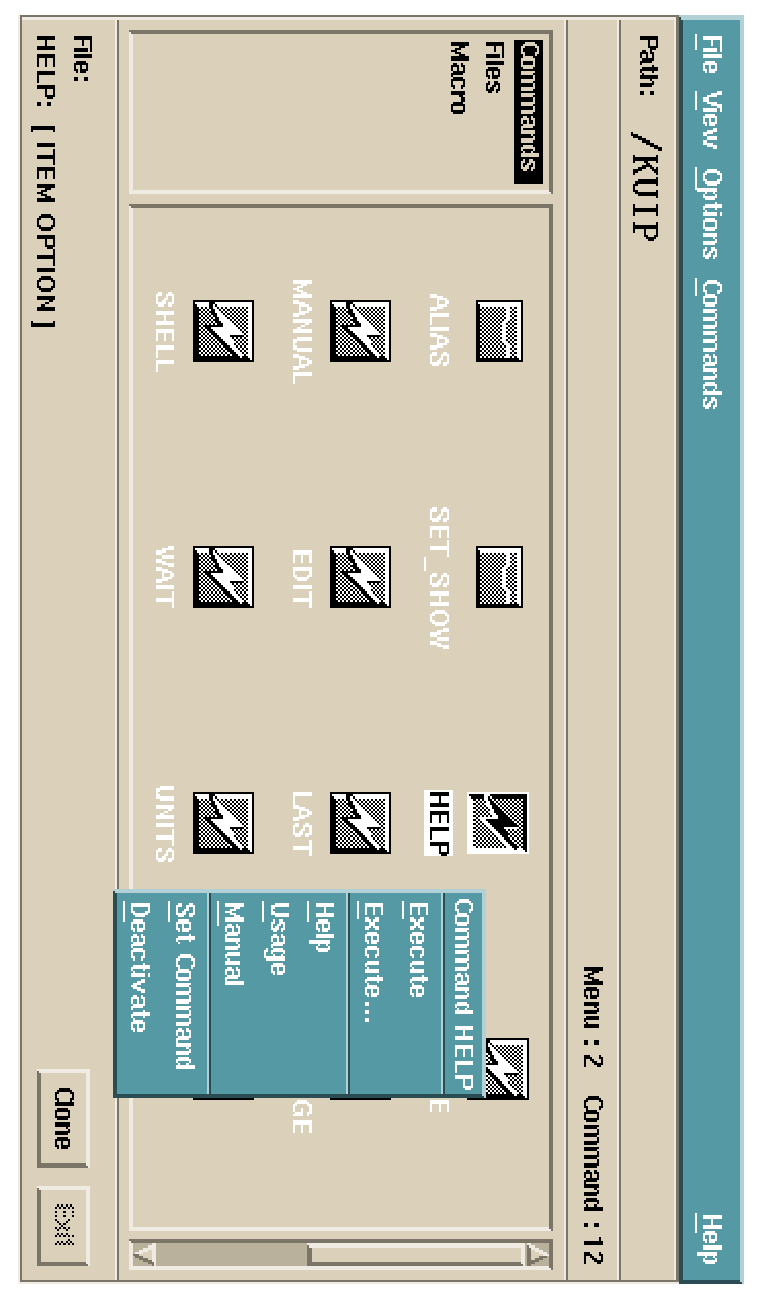
\epsfig{file=browser.eps,height=\textwidth}
\end{sideways}
\caption{\KUIPMotif{} object browser.
\label{fig-motif-browser}}
\end{figure}

\subsection{Browser terminology}

The main part of the browser (figure~\ref{fig-motif-browser})
is taken by the \textem{content window} to display \textem{objects} as 
\textem{icons}.
Each object is identified by its \textem{name} and its type or \textem{class}.
The \Lit{>Class} directive defines new classes and determines the
icons to be used for displaying the objects.

The objects are attached to container objects called \textem{browsables}.
Browsables are identified by a name and a class as well.
The \textem{class window} to the left of the content window displays the
list of browsables known to the browser.
The \Lit{>Browse} directive has to give for each browsable class a 
\textsl{next-object} routine which has to be provided by the application.
The browser calls this routine in order to retrieve the list of
objects which should be displayed in the content window.

A browsable can also contain a tree structure of objects by defining a
special object class for \textem{directories} containing other objects.
The browser keeps track of the current directory path for each
browsable.
The current path for the selected browsable is displayed in the 
\textem{path window} above the class window.
When changing into a subdirectory the new directory path is formed by
concatenating the old path, a ``\Lit{/}'', and the name of the
directory object.
This new directory path is then passed to the \textsl{next-object}
routine in order to retrieve the objects contained in the
subdirectory and to update the content window.

\subsection{The ``next-browsable'' routine}

In frequent cases browsables are stored in external files and a
variable number of them can be connected to the browser.
The \Lit{Browse} directive allows to specify a \textsl{next-browsable}
routine to retrieve the list of currently connected browsables from the
application.

\begin{figure}[tb]
\begin{XMP}
      SUBROUTINE next_browsable(
     +   browsable_name, browsable_class, meta_variables )
      CHARACTER*(*) browsable_name, browsable_class, meta_variables
         ...
      SAVE next_counter

      IF( browsable_name .EQ. ' ' ) THEN
         next_counter = 1
      ELSE
         next_counter = next_counter + 1
      ENDIF

*--- find <next_counter> browsable of requested browsable_class
         ...

      IF( no_more_browsables_left ) THEN
         browsable_name = ' '
      ELSE
         browsable_name = ...
         meta_variables = ...
*--- e.g. 'root=//LUN1 unit=1 file=myfile.hbook'
      ENDIF
      END
\end{XMP}
\caption{Skeleton for a \textsl{next-browsable} routine in Fortran.
\label{fig-next-browsable}}
\end{figure}

The \textsl{next-browsable} routines are iterator functions, i.e.\ they
have to return one browsable at a time.
Figure~\ref{fig-next-browsable} shows the skeleton for a 
\textsl{next-browsable} routine in Fortran.
For each browsable class the browser calls the corresponding routine
in a loop. 
Before the first call \Lit{browsable_name} is set to blank and the
loop continues until the returned \Lit{browsable_name} is blank again.

The second argument \Lit{browsable_class} is set to the name of the
browsable class defined by the \Lit{>Browse} directive.
The same \textsl{next-browsable} routine may be used for several
browsable classes by identifying the currently requested class from
\Lit{browsable_class}. 
It is save to do the class identification only once at the first iteration,
i.e.\ when \Lit{browsable_name} is blank on entry.

If the call to \textsl{next-browsable} returns with a non-blank value in
\Lit{browsable_name} a browsable with the give name is added to the
class window.
The output argument \Lit{meta_variables} should contain a blank
separated list of ``\textsl{var}\texttt{=}\textsl{value}'' \textem{meta-variable}
definitions. 



Browsable classes without a \textsl{next-browsable} routine are called
\textem{single-instance} and are pre-connected to the browser.


\subsection{Action menus}

\if0

of the given class which
should be displayed 
can add to the \Lit{File} menu
in the browser's top menu bar actions
Each browsable class in the class window.
an action menu to operate
on the currently selected browsable.

contained in a
n application-supplied
browsable. 

 and the menus from which an \textem{action} on the selected object
can be chosen. 

 and most of the \Motif{}-specific \CDF{} directives deal with the
customization of the browser.
An application can define in the \CDF{} new types of objects 
(\textem{classes}) to be accessible by the browser.

The selected object (command \Lit{HELP}) is high-lighted and pressing
the right-hand mouse button pops up an \textem{action menu}.
The icons and action menus depend on the object \textem{class} and have
to be defined in the \CDF{}.

The objects are contained in \textem{browsables}
The \textem{class window} to the left of the content window 

The class definition also has to specify a routine which the browser
can call to retrieve the objects contained in the current directory.
This routine has to return the \textem{class name} ``\Lit{Command}'' and
the \textem{object name} ``\Lit{HELP}'' (which must be unique within the
current directory). 
Each item in an action menu allows to specify a \textem{command sequence}
to be executed.
The \textem{meta-variable} ``\Lit{[this]}'' in the command sequence is
replaced by the name of the selected object.

Each object can have two additional attributes: a short and a long
description text.
The meta-variable ``\Lit{[that]}'' refers to the short text and allows
to use it as \textem{object alias}.
The long text ``\Lit{[ ITEM OPTION ]}'' and the name of the selected
object is displayed in the \textem{object description} at the bottom of
the browser. 
The ``\Lit{View}'' pull-down menu allows to choose between different
ways of displaying the objects in the content window:
\begin{UL}
\item Big icons and object name
\item Small icons and object name
\item Object name and short text (no icons)
\item Small icons, object name, short text, and long text
\end{UL}
The vertical scroll bar to the right of the content window allows to
see different sections of the content window.
The total object count ``\Lit{Menu : 2  Command : 12}'' is displayed
in the \textem{summary line} just above the content window.


Directories are a special object class 


\begin{Gray}{i}
>BROWSE  class-name  title-text  next-object  next-browsable
\end{Gray}
The \Lit{>Browse} directive defines a browsable class 
\textsl{class-name}.
\textsl{Title-text} is used for the pop-up menu header in the class
window.
\textsl{Next-object} and \textsl{next-browsable} are the names of routines
which have to be supplied by the application.
\textsl{Next-object} is called by the browser in order to retrieve the
objects contained in a browsable. 
\textsl{Next-browsable} is called to retrieve the list of connected
browsables. 
In simple cases a \textsl{next-browsable} routine need not be defined
(see below).


The \Lit{>Browse} directive is followed by two action lists
separated by a line containing on a ``\Lit{+}'' character in the first
column: 
\begin{XMP}
\textsl{action list for class window}
+
\textsl{action list for {\tt File} menu}
\end{XMP}
The action lists define the menus of possible actions with
each line containing the fields:

\indent\indent\begin{tabular}{cccc}
\textsl{menu-text} &  $[$ \textsl{option-flags} & \textsl{command-sequence}
& \textsl{call-back-routine} $]$
\end{tabular}
\vskip\parskip

The fields are positional separated by blanks.
A field value containing embedded blanks must be enclosed in quotes.
Empty fields have to specified as a single ``\Lit{.}'' character.
Empty fields at the end of a line may be omitted.

\textsl{Menu-text} is the text which will be displayed in the menu.
\textsl{Option-flags} can contain the special characters:
\begin{UL}
\item ``\Lit{/}'' to insert a separator line above the menu item.
\item ``\Lit{!}'' to flag actions which create or delete objects.
This option is required to force updating all browser windows which
could be affected by a change in the object content.
\end{UL}

\textsl{Command-sequence} allows to defines a command string which should be
executed when the corresponding menu item is selected.
The command string can contain several commands separated by
``\Lit{;}''.
The semicolon should be followed by a blank to avoid the exception
rules when ``\Lit{;}'' is not treated as a command separator.
Meta-variables ``\Lit{[}\textsl{var}\Lit{]}'' inside the command string
allow to refer to the selected browsable.
They are replaced by the values defined by the \textsl{next-browsable}
routine (see below for the meta-variables with a predefined meaning).

After replacing the meta-variables the commands are executed as if
they were typed in. 
Command names may be abbreviated but should at least contain a partial
menu path to avoid conflicts if the user defines aliases or changes
the command root with \Lit{SET/ROOT}. 
A command provided with all mandatory arguments is usually executed
immediately. 
The immediate execution can be inhibited by preceding the command name
with a ``\Lit{-}''~character.
As in the case of missing mandatory arguments the ``\Lit{-}'' forces the
display of the corresponding command panel derived from the \CDF{} (see
figure~\ref{fig-motif-panel}). 

\begin{figure}[htb]
\begin{sideways}
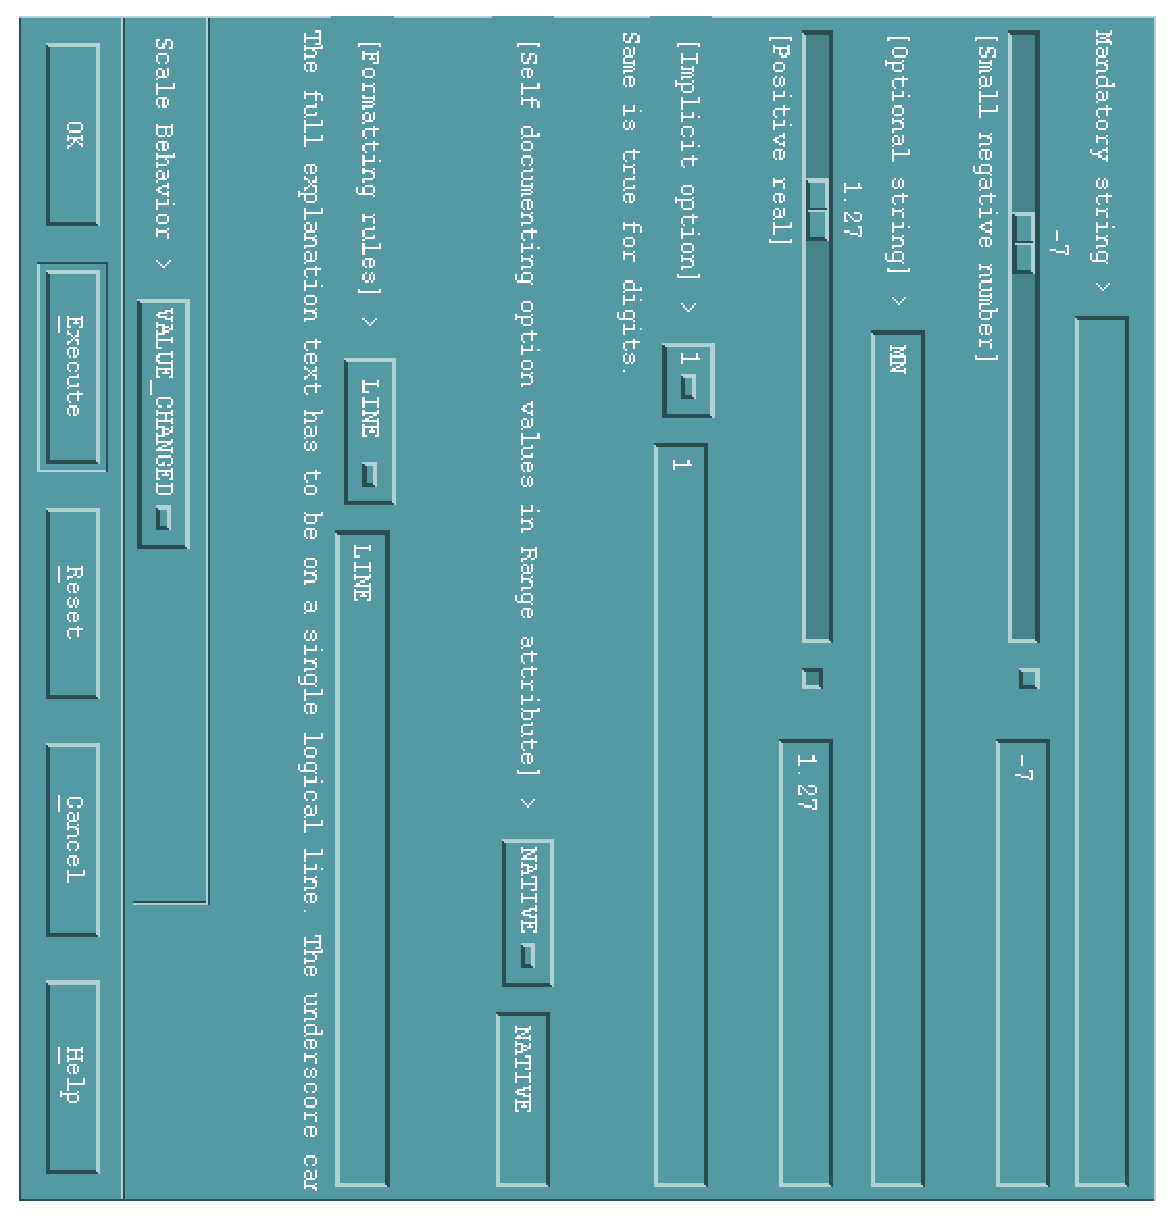
\epsfig{file=xechopanel.eps,height=.47\textwidth}
\end{sideways}
\hspace{\fill}
\begin{sideways}
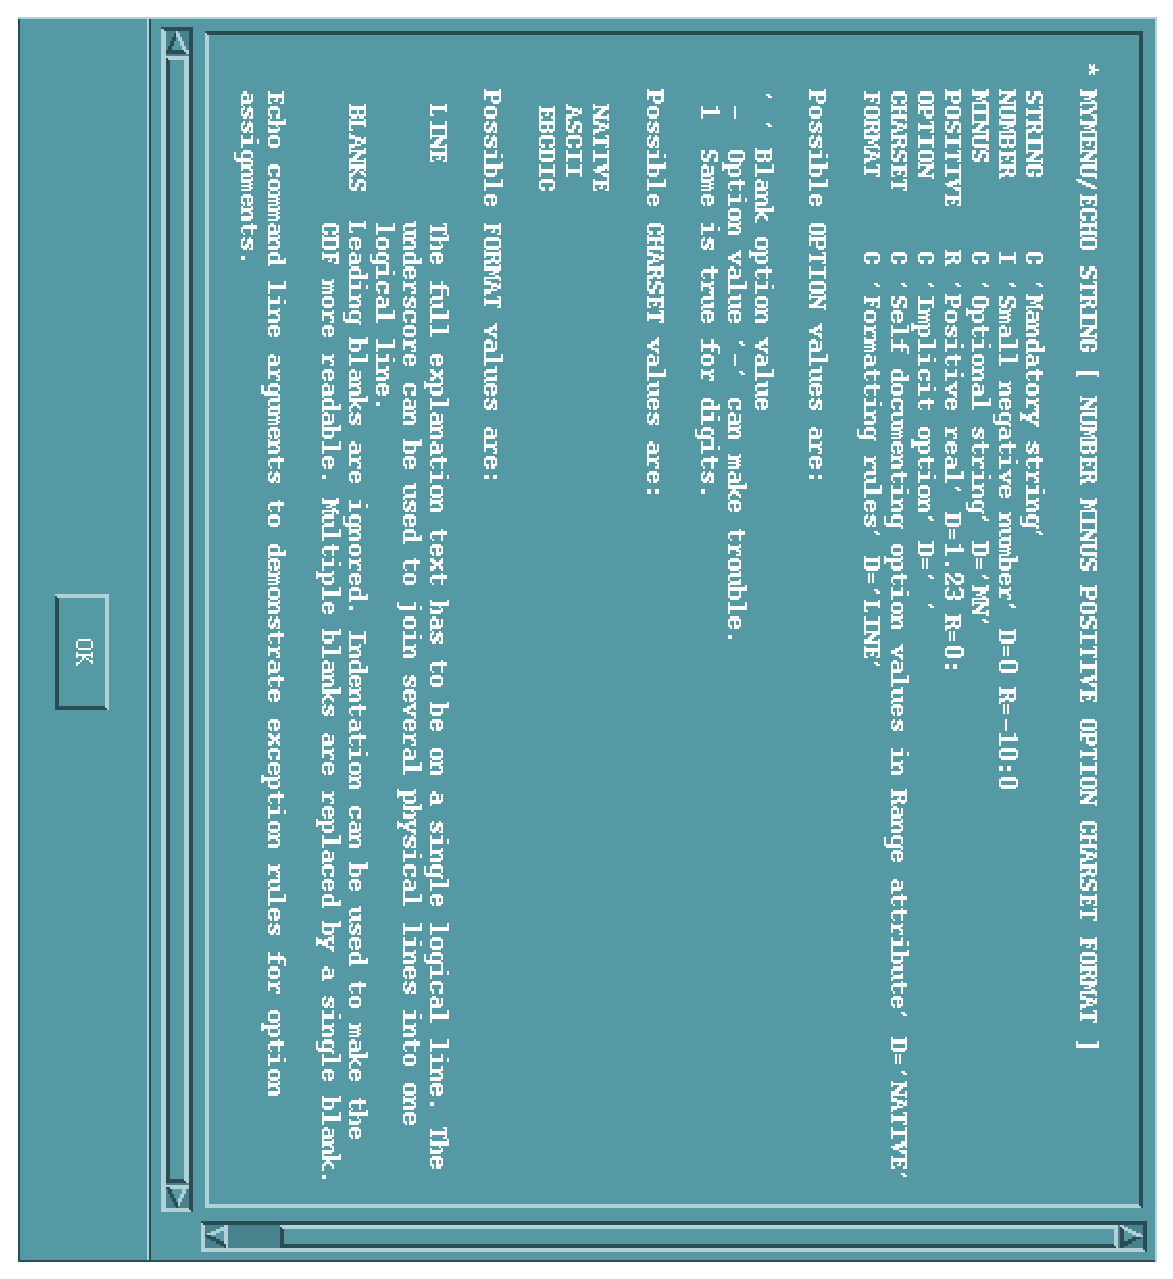
\epsfig{file=xechohelp.eps,height=.49\textwidth}
\end{sideways}
\caption{\Motif{} command panel and help window from \CDF{} example.
\label{fig-motif-panel}}
\end{figure}

The panel allows the user to fill in or change argument values before
executing the command.
The ``\Lit{-}'' should also be used for destructive commands 
(e.g.\ delete object or close file) to allow the user to cancel the execution.
Each panel provides five buttons:
\begin{UL}
\item \Lit{OK} executes the command and destroys the panel.
\item \Lit{Execute} executes the command but keeps the panel for
further command executions.
\item \Lit{Reset} resets all parameters to their default values.
\item \Lit{Cancel} destroys the panel without executing the command.
Further commands in the same \textsl{command-sequence} are ignored.
\item \Lit{Help} displays the help text in a separate window.
\end{UL}
To ensure the sequential execution of a command sequence the \Motif{}
event loop is blocked for all but the last command, i.e.\ 
the user has to press either the \Lit{OK} button or the \Lit{Cancel}
button before the application can continue.

The user can also force the panel display for each command in the
sequence by holding the \Lit{CTRL}-key before popping\footnote{
The \Motif{} implementation of pop-up menus does not allow to sense key
presses during the pop-up display.}
the menu.
The user-forced panel display can be inhibited by preceding the
command name by a ``\Lit{+}''~character.
This should be used in sequences where changing the arguments may
jeopardize the successful execution of subsequent commands, e.g.\ for
a directory change followed by a command using a relative path only.
Obviously the corresponding ``\Lit{+}''~command has to be provided with all
mandatory arguments in order to be executable.

For special applications the action line may also define a 
\textsl{call-back-routine} to be called when the corresponding menu item
is selected. 
(If a \textsl{command-sequence} is defined as well the \textsl{call-back-routine}
is called after executing the commands.)
\textsl{Call-back-routine} may either be the name of a Fortran routine or
the name of C~function followed by ``\Lit{\%C}''.
For a Fortran routine the calling sequence depends on the
action menu for which it is defined (see below).



In addition or as an alternative to a command sequence 

For sequences where subsequent commands depend on that


 of and some arguments may be omitted.

The command definitions explained in the previous section are used by
the \KUIPMotif{} interface to generate command panels where the user can
fill in missing arguments or change default values.
Figure~\ref{fig-motif-panel} shows the panel created automatically
from the \Lit{ECHO} command example.


A minimum set of meta-variables has to be defined by the 
\textsl{next-browsable} routine:
\begin{UL}
\item \Lit{[name]} as the name of the browsable.
\item \Lit{[root]} as the initial setting for \Lit{[path]}.
\item \Lit{[file]} as the text which should be displayed at the bottom
of the browser.
\end{UL}

Note that all fields in an action line are positional 

 to contains a ``\Lit{/}'' character 

The first action list defines the pop-up menu for the browsable selected
in the class window.
The second action list add items to the \Lit{File} pull-down menu.
This allows to define to define the necessary actions to connect
browsables which are stored in external files.

is a browsable class 
\textsl{class-name}.

Figure~\ref{fig-next-object} shows the skeleton for 
\fi

\begin{figure}[htb]
\begin{XMP}
      SUBROUTINE next_object(
     +   browsable_name, browsable_class, current_path,
     +   object_name, object_class, short_text, long_text )
      CHARACTER*(*) browsable_name, ..., long_text
         ...
      SAVE next_counter

      IF( object_name .EQ. ' ' ) THEN
*--- first object is requested
         next_counter = 1

*--- identify from browsable_name, browsable_class
*--- and current_path which objects are requested
            ...
      ELSE
*--- next object is requested
         next_counter = next_counter + 1
      ENDIF

*--- find object with number next_counter
         ...

      IF( no_more_objects_left ) THEN
*--- stop scanning process
         object_name = ' '
      ELSE
*--- mandatory return values
         object_name = ...
         object_class = ...

*--- optional return values
         short_text = ...
         long_text = ...
      ENDIF
      END
\end{XMP}
\caption{Skeleton for the \textsl{next-object} routine.
\label{fig-next-object}}
\end{figure}

\if0
and is followed
by the menu definitions
\begin{XMP}\tt
\textsl{action list for class window} 
+ 
\textsl{action list for File menu}
\end{XMP}

the routine which should be called after decoding the command line in
order to perform the intended operations.

%\end{minipage}


\section{Example of \CDF{} files}

Below we list an example of a \CDF{} (being in fact the first part of the \CDF{} of PAW),
and the corresponding Fortran code generated by the \KUIP{} Compiler.
%
%---------------------------------------------------------------------------
%
\begin{XMPtext}{Example of a \CDF{} file}
>Name HISDEF
 
>Menu HISTOGRAM
>Guidance
Manipulation of histograms, Ntuples.
Interface to the HBOOK package.
 
>Command FILE
>Parameters
LUN 'Logical unit number' I R=1:128
FNAME 'File name' C
+
LRECL 'Record length in words' I D=1024
CHOPT 'CHOPT' C D=' ' R=' ,N,U'
>Guidance
Open an HBOOK direct access file.
 For CHOPT=' ', existing file opened (read only).
 For CHOPT='N', a new file is opened.
 For CHOPT='U', existing file opened to be modified.
>Action PAHIST
 
>Command LIST
>Parameters
+
CHOPT 'Options' C D=' ' R=' ,I'
>Guidance
List the histograms in the current directory (memory or disk).
Histograms are all HBOOK objects including Ntuples.
If CHOPT='I' a verbose format is used (batch: HINDEX).
>Action PAHIST
\end{XMPtext}
\newpage
\begin{XMPtext}{Fortran code generated from the \CDF{}}
*     -------------------
      SUBROUTINE HISDEF
*     -------------------
      INTEGER MGUIDL
      PARAMETER (MGUIDL=199)
      CHARACTER*80 GUID
      COMMON /KCGUID/ GUID(MGUIDL)
      EXTERNAL PAHIST
      EXTERNAL HISDEH
 
      CALL KUNWG(  -1)
      CALL KUCMD(' ','HISTOGRAM','C')
      CALL KUACG('HISTOGRAM',HISDEH)
      CALL KUCMD('HISTOGRAM',' ','SW')
 
      CALL KUNWG(  -2)
      CALL KUCMD(' ','FILE','C ')
      CALL KUNDPV(  1,  1,  1,  0,  1)
      CALL KUPAR('FILE','LUN','Logical unit number','I ','S')
      CALL KUPVAL('FILE','LUN',1,0.,' ','L')
      CALL KUPVAL('FILE','LUN',128,0.,' ','H')
      CALL KUNDPV( 1, 1, 1, 0,  1)
      CALL KUPAR('FILE','FNAME','File name','C ','S')
      CALL KUNDPV(  1,  1,  1,  0,  1)
      CALL KUPAR('FILE','LRECL','Record length in words','IO','S')
      CALL KUPVAL('FILE','LRECL',1024,0.,' ','D')
      CALL KUNDPV( 1, 1, 1, 1,  2)
      CALL KUPAR('FILE','CHOPT','CHOPT','CO','S')
      CALL KUPVAL('FILE','CHOPT',0,0.,' ,N,U','V')
      CALL KUPVAL('FILE','CHOPT',0,0.,' ','D')
      CALL KUACG('FILE',HISDEH)
      CALL KUACT('FILE',PAHIST)
 
      CALL KUNWG(  -3)
      CALL KUCMD(' ','LIST','C ')
      CALL KUNDPV( 1, 1, 1, 1,  1)
      CALL KUPAR('LIST','CHOPT','Options','CO','S')
      CALL KUPVAL('LIST','CHOPT',0,0.,' ,I','V')
      CALL KUPVAL('LIST','CHOPT',0,0.,' ','D')
      CALL KUACG('LIST',HISDEH)
      CALL KUACT('LIST',PAHIST)
 
      CALL KUNWG(   0)
      CALL KUNDPV(   1,   1,   1,   0,   1)
      CALL KUCMD(' ',' ','E')
      CALL KUCMD('/',' ','SW')
      END
*     -------------------
      SUBROUTINE HISDEH
*     -------------------
      INTEGER MGUIDL
      PARAMETER (MGUIDL=199)
      CHARACTER*80 GUID
      COMMON /KCGUID/ GUID(MGUIDL)
      COMMON /KCGUIL/ NGLN
*
      GOTO( 1, 2, 3),NGLN
*
* HISTOGRAM
*
    1 CONTINUE
      GUID( 1)='Manipulation of histograms, Ntuples. '
      GUID( 2)='Interface to the HBOOK package. '
      NGLN=  2
      GOTO 9999
*
* HISTOGRAM/FILE
*
    2 CONTINUE
      GUID( 1)='Open an HBOOK direct access file. '
      GUID( 2)=' For CHOPT='' '', existing file opened (read only).'
      GUID( 3)=' For CHOPT=''N'', a new file is opened. '
      GUID( 4)=' For CHOPT=''U'', existing file opened to be modified.'
      NGLN=  4
      GOTO 9999
*
* HISTOGRAM/LIST
*
    3 CONTINUE
      GUID( 1)='List the histograms in the current directory (memory or
     +disk). '
      GUID( 2)='Histograms are all HBOOK objects including Ntuples. '
      GUID( 3)='If CHOPT=''I'' a verbose format is used (batch: HINDEX).
     + '
      NGLN=  3
      GOTO 9999
9999  RETURN
      END
\end{XMPtext}
%
%---------------------------------------------------------------------------
%
\fi
\fi

\section{Various Hints specific to \KUIPMotif{}}
 
\subsection{ C-callable Interface to the Panel Interface}
 
A C-callable interface for the complete \Cind{PANEL} interface (panels and
palettes) built-in inside \KUIPMotif{} (see \ref{ref:repanel})
is accessible to the application programmer. This allows him
to set up some predefined panels without having to transport
independent macro files together with the application executable,
and having to refer them in the logon macro file.
This is the case, for example,  of the graphical editor ``Ged'' which makes
an intensive use of graphical and alphanumerics ``programmer-defined''
panels.
 
The C callable entries are:

\begin{Gray}{l}
void km_panel_reset()
\end{Gray}
Reset panel in memory (<>~``\Lit{panel 0 r}'').

\begin{Gray}{l}
void km_panel_key( int row, int col,  char *command, 
                   char *alias_label, char *pixmap )
\end{Gray}
\Pdesc\begin{DLtt}{\mbox{\hspace{7em}}}
\item[row] row number
\item[col] column number
\item[command]  command (or list of commands) to be executed
\condbreak{2\baselineskip}
\item[alias_label] alias name for command (or NULL)
\item[pixmap] pixmap representation for button label (or NULL)
\end{DLtt}
Define key (<>~``\Lit{panel x.y ...}'').

\begin{Gray}{l}
void km_panel_display( char *title, char *geometry )
\end{Gray}
\Pdesc\begin{DLtt}{\mbox{\hspace{7em}}}
\item[title] panel title
\item[geometry] panel geometry
  (\textsl{w}\texttt{x}\textsl{h}\texttt{+}\textsl{x}\texttt{+}\textsl{y}) 
\end{DLtt}
Display panel (<>~``\Lit{panel 0 d ...}'').

\begin{Gray}{l}
void km_panel_close( char *title )
\end{Gray}
\Pdesc\begin{DLtt}{\mbox{\hspace{7em}}}
\item[title] panel title
\end{DLtt}
Close panel with given title (<>~``\Lit{panel 0 c ...}'').

\begin{Gray}{l}
void km_icon( char *icon, char *fname )
\end{Gray}
\Pdesc\begin{DLtt}{\mbox{\hspace{7em}}}
\item[icon] icon name
\item[fname] filename (output of the X11 utility bitmaps).
\end{DLtt}
Store icon data from a bitmap file (<>~``\Lit{motif/icon ...}'').

\begin{Gray}{l}
void km_palette( char *title, char *geometry )
\end{Gray}
\Pdesc\begin{DLtt}{\mbox{\hspace{7em}}}
\item[title] palette title
\item[geometry] palette geometry (wxh+x+y)
\end{DLtt}
Open or close a ``multi-panel'' (palette) widget
(<>~``\Lit{motif/multi_panel ...}'').
 
The routine (written by the application programmer) which contains
all the panels definition has to be called via the ``Motif\_customize''
mechanism (described is section \ref{ref:rehooks}) in the so-called
``widget-routine'' (its has to be called before entering the Motif
main loop, but after initialization).
 
E.g.:
\begin{XMP}
>Motif\_customize . init_top_level_window%C
\end{XMP}
 
The following is an illustration of how to use these routines. On
the left side you have the KUIP macro file for a panel definition, and
on the right side you have the equivalent coded in~C. The C~routine
\texttt{my_panel_definition} is automatically called by KUIP,
just after the creation of the \EW{} (kxterm), thanks
to the \CDF{} directive ''Motif\_customize''.
(See the code of the ``widget-routine'' \texttt{init_top_level_window} at the end
of the ``C~Interface'' side).
\vfill 
\begin{XMP}
**************           |     /***************/
* KUIP Macro *           |     /* C Interface */
**************           |     /***************/
 
                         |     #include <X11/Intrinsic.h>

                         |     extern void km_icon();
                         |     extern void km_panel_reset();
                         |     extern void km_panel_display();
                         |     extern void km_panel_key();

                         |     my_panel_definition()
                         |     \{
*
* Icon bitmaps
*
/motif/icon m1 mk1.bm    |       km_icon ("m1", "/user/cremel/ktest/mk1.bm");
/motif/icon m2 mk2.bm    |       km_icon ("m2", "/user/cremel/ktest/mk2.bm");
/motif/icon m3 mk3.bm    |       km_icon ("m3", "/user/cremel/ktest/mk3.bm");
/motif/icon m4 mk4.bm    |       km_icon ("m4", "/user/cremel/ktest/mk4.bm");
/motif/icon m5 mk5.bm    |       km_icon ("m5", "/user/cremel/ktest/mk5.bm");
 
*
* Panel keys definition
*
panel 0                  |       km_panel_reset();
panel 2.01 null          |       km_panel_key (2, 1, "null", NULL, NULL);
panel 2.02 tex_1         |       km_panel_key (2, 2, "tex_1", NULL, NULL);
panel 3.01 '/example/general kuip.tex tex 1' 'tex_1' m1
                         |       km_panel_key (3, 1, ...
                           ..."/example/general kuip.tex tex 1", "tex_1", "m1");
panel 3.02 '/example/general kuip.tex tex 2' 'tex_2' m2
                         |       km_panel_key (3, 2, ...
                           ..."example/general kuip.tex tex 2", "tex_2", "m2");
panel 3.03 '/example/general kuip.tex tex 3' . m3
                         |       km_panel_key (3, 3, ...
                           ..."example/general kuip.tex tex 3", NULL, "m3");
panel 3.04 '/example/general kuip.tex tex 4' . m4
                         |       km_panel_key (3, 4, ...
                           ..."example/general kuip.tex tex 4", NULL, "m4");
panel 4.01 ' ' . m5      |       km_panel_key (4, 1, " ", NULL, "m5");
panel 4.02 'tex_5' . m5  |       km_panel_key (4, 2, "tex_5", NULL, "m5");
panel 5.01 '/example/general kuip.tex tex 6' . m6
                         |       km_panel_key (5, 1, ...
                           ..."example/general kuip.tex tex 6", NULL, "m6");\condbreak{3\baselineskip}
panel 5.02 '/example/general kuip.tex tex 6' . big_menu
                         |       km_panel_key (5, 2, ...
                           ..."example/general kuip.tex tex 6",NULL,"big_menu");
panel 6.01 '/example/general kuip.tex tex 7' 'tex_7'
                         |       km_panel_key (6, 1, ...
                           ..."example/general kuip.tex tex 7", "tex_7",NULL);
panel 6.02 '/example/general kuip.tex tex 7' 'tex_7' m1
                         |       km_panel_key (6, 2, ...
                           ..."example/general kuip.tex tex 7", "tex_7", "m1");
 
* Open a palette (multi_panel)
multi_panel 'Marker Palette' '300x1000-0+0'
                         |       km_palette ("Marker Palette", "300x1000-0+0");
 
* Display panel(s)
panel 0 d 'Marker Types' 300x300+500+500
                         |       km_panel_display ("Marker Types", ...
                           ..."300x300+500+500");
 
* Close current palette
multi_panel 'end'        |       km_palette ("end", NULL);
                         |     \}
 
                         |     void init_top_level_window(name, top)
                         |         char *name;
                         |         Widget top;
                         |     \{
                         |       if (strcmp(name,"kxterm") == 0) \{
                         |         my_panel_definition();
                         |       \}
                         |     \}
\end{XMP}
 
 
\subsection{User-Defined Single Selection Lists}
 
It is possible in \KUIPMotif{} to set up a command which displays a
list of various items or choices (instead of the usual command
argument panel with the list of arguments to be filled).
This is,
for instance, the behavior of the command ``HELP'' in \KUIPMotif{}:
if you type ``help'' without any argument a selection box with all
possible help menus or items is displayed and the user can select
one (or just cancel the execution) and get the appropriate help information.
 
Note that the argument type ``list'' does not exist in the basic
\KUIP{} and we thought that the most frequent case is probably
the one mentioned above, i.e.\ a command which displays a predefined list
(or set up at run time). In such a case one should get access
to the ``Selection Box'' widget in a so-called Motif interface.
 
To implement such a command the application-programmer has to define
in the CDF (with the other application defined commands) a new command
without any argument and the action routine written in~C. 
E.g.:
\begin{XMP}\condbreak{2\baselineskip}
>Menu EXAMPLE
...
>Command LIST
>Guidance
This is just an example of a command which
displays a list of items.
(See action routine ktactc.c)
>Action ktactc%C
\end{XMP}
We provide in \KUIPMotif{} two user-callable C~routines (\texttt{km_list_data}
and \texttt{km_show_list} which make the implementation of this ``list display''
quite easy (no Motif code is involved). These routines have to be called
directly in the code of the action routine. The part which concerns the
filling of the list and the action to execute after a selection has been
done (<OK> button pressed) is (obviously) application dependent.
 
Description of these two user-callable C~routines:

\begin{Gray}{i}
void km_list_data( char *list_label, char *selection_label,
                   char *help_text,  int call_back(char* selection) )
\end{Gray}
\Pdesc\begin{DLtt}{\mbox{\hspace{7em}}}
\item[list_label]  label (prompt) written at the beginning of the list
\item[selection_label]  label (prompt) written before the selection
\item[help_text]  help message accessed through help button
\item[call_back]  user defined routine called when the OK is pressed.
  The value selected by the user is passed as argument when the
  routine is called.
\end{DLtt}
Fill the application data for a user-defined list.
All parameters are application dependent.

 
\begin{Gray}{i}
void km_show_list( char **items )
\end{Gray}
\Pdesc\begin{DLtt}{\mbox{\hspace{7em}}}
\item[items]  list of items (choices) in the list.
\end{DLtt}
Displays the list.
 
The following is a skeleton (some parts have to be filled according to
the application) for the application routine \texttt{ktactc.c} for the
new command ``LIST'' described above:
\begin{XMP}
/* Listing of file ktactc.c */
 
#ifndef NULL
#define NULL 0
#endif
 
/***************************************************************/
/*                                                             */\condbreak{3\baselineskip}
/* Action routine for command "/EXAMPLE/LIST"                  */
/* (Example of how to display a "user defined" list            */
/*  with KUIP/Motif).                                          */
/*                                                             */
/***************************************************************/
 
ktactc()
\{
  int ktactc_OK ();
  int i;
 
  static char *help_text = "You can write there \bs{}n\bs{}
some help text for \bs{}"My List\bs{}" ...";
 
  /* List of all items (can be filled dynamically) */
  char **list_item = (char **) malloc ( sizeof (char *) );
 
  /* Fill list data: */
  km_list_data
     ("My List Label", "My List Selection", help_text, ktactc_OK);
 
  /* Fill list of items (with 10 arbitrary values) ...
   * ... N.B. Write your application defined code here ... i
   */
  for (i = 0; i < 10; i++) \{
       list_item = (char **) realloc( (char*)list_item,
                                        (i+1) * sizeof (char *) );
       list_item[i] = (char *) malloc (10);
       sprintf (list_item[i], "item %d", i+1);
  \}
  list_item = (char **) realloc( (char*)list_item, (i+1) * sizeof (char *) );
  list_item[i] = NULL;
 
  /*
   * Display list and wait for user action ...
   * ... N.B. If user action is "OK" you go into
   * the "OK call-back" defined by km_list_data (ktactc_OK)
   * - See example for code of ktactc_OK above _
   */
  km_show_list (list_item);
 
  for (i = 0; i < 10; i++) free (list_item[i]);
  free (list_item);
\}
\vfill 
/*
 * Routine name (ktactc_OK) is defined by KM_list_data.
 * This routine is automatically called when pressing the "OK" button.
 *      char *val (input) : value issued from the user selection
 *
 */
int ktactc_OK (val)
    char *val;
\{
    printf ("*** display_list_OK : (ktactc_OK)\bs{}n");
    printf ("    value selected in the list %s.\bs{}n", val);
 
    return 0;
\}
\end{XMP}
 
Picture \ref{ref:FIGPKMF192} shows the output from
\KUIPMotif{} when executing the command ``/EXAMPLE/LIST'' described above.

\begin{figure}[htb]
\hfill
\begin{PICTf}[.4]{pkmf192}
\end{PICTf}
\hfill
\caption{User-defined List in a Command}
\label{ref:FIGPKMF192}
\end{figure}
 
\subsection{User-Defined File Selection Boxes}
 
It is also possible with \KUIPMotif{} to set up a command which displays a
"FileSelectionBox" (conform to the Motif terminology) containing:
\begin{UL}
\item
a ``Filter'' entry to select only files with a certain pattern,
\item
a ``Directories'' entry to select the directory applied to the ``Filter''
(this can also be done by editing the ``Filter'' entry manually),
\item
a ``Files'' entry, with the list of all files corresponding to the
``Filter'' selected.
\end{UL}
This is a very convenient way to select a file name, and being able to
scan the directory tree.
 
To implement such a command the application-programmer has to define
in the CDF (with the other application defined commands) a new command
without any argument and the action routine written in C. E.g.:
\begin{XMP}
>Menu EXAMPLE
...
>Command SELECT_FILE
>Guidance
This is just an example of a command which
displays a file list selection box.
(See action routine ktactcf.c)
>Action ktactcf%C
\end{XMP}
We provide the user-callable a C~routine (\Lit{km_show_filSel})
which makes the implementation of this ``FileSelectionBox''
quite easy (no Motif code is involved). It has to be called
directly in the code of the action routine. The part which concerns the
data setting and the action to execute after a selection has been
done (<OK> button pressed) is (obviously) application dependent.
 
N.B. You get automatically to this "FileSelectionBox" by defining a
parameter type ``FILE'' (extension to the type ``\Lit{C}'' (character) in the
\CDF{}). But this C user-callable routine
gives the application programmer the
possibility to define commands that directly display a
"FileSelectionBox" (without producing the usual ``Command Argument Panel'')
and also to fill the data (filter, default value) at run time.
 
Description:
\begin{Gray}{i}
void km_show_filSel( char *title, char *dir, char *def, char *help,
                     int call_back(char* selection) )
\end{Gray}
All parameters (input) in this routine are application dependent.
\Pdesc\begin{DLtt}{\mbox{\hspace{7em}}}
\item[title] title of the FileSelectionBox
\item[dir] directory (for filter)
\item[def] default file name
\item[help] help text (accessed through help button)
\item[call_back]  user defined routine called when the ``OK'' button
  is pressed. 
  The value selected by the user is passed as argument when the
  routine is called.
\end{DLtt}
 
The following is a skeleton (some parts have to be filled according to
the application) for the application routine \texttt{ktactcf} for the
new command \Cind{SELECT_FILE} described above:
\begin{XMP}
/* ktactcf.c */
 
#include <stdio.h>

extern void km_show_filSel( char *title, char *dir, char *def, char *help,
                            int callback(char* selection) );


/*
 * This routine is automatically called when pressing the "OK" button.
 *      char *val (input) : value issued from the user selection
 */
int ktactcf_OK( char *val )
\{
    printf( "*** fileSelection OK : (ktactcf_OK)\bs{}n" );
    printf( "    File selected is %s.\bs{}n", val );\condbreak{2\baselineskip}
    return 0;
\}
 

/*
 * Action routine for command "SELECT_FILE".
 * (Example of how to display a "user defined" file selection
 *  box with KUIP/Motif).
 */
int ktactcf()
\{
\condbreak{2\baselineskip}
  static char *help_text = "You can write there \bs{}n\bs{}
some help text for \bs{}"My FileSelectionBox\bs{}" ...";
 
    km_show_filSel( "My FileSelectionBox",
                    "/user/cremel/pdemo/*.dat", "hrztest.dat",
                    help_text, ktactcf_OK );
    return 0;
\}
\end{XMP}
 
Picture \ref{ref:FIGPKMF193} shows the output from
\KUIPMotif{} when executing the command \Cind{SELECT_FILE} described
above.

\begin{figure}[htb]
\hfill
\begin{PICTf}[.4]{pkmf193}
\end{PICTf}
\hfill
\caption{User-defined File Selection Box in a Command}
\label{ref:FIGPKMF193}
\end{figure}
 
 
 
\section{Some Examples to Start With}

\subsection{Example 1: Basic Example (No Graphics)}
\label{ref:reexnogr}

This first example is a very simple one in order to show 
\begin{OL}
\item how the different types of parameters handled by \KUIP{} are interpreted 
and visualized in the \Motif{} interface (\CAP{}).
\item what you automatically get with \KUIPMotif{}.
\end{OL}

\subsubsection{The \CAP{} for a Very General Command}

The following \CDF{} defines a new menu ``Example'' and a new command
''General'' with 6 input parameters. The first 2 parameters are mandatory 
and the others are optional.

The action routine to be called at command execution is named KTACT.

\condbreak{3cm}
\begin{XMPt} {Example 1 --- \CDF{} (Command Definition File) ---
ktcdf.cdf}
>Name KTDEF

>Menu Example

>Command General
>Parameters
FILE 'File name' C D='kuip.tex'
OPTION 'Text formatting system' C D='TEX'
-      plain text : plain text format
-LATEX LaTeX format (encapsulated)
-TEX   LaTeX format (without header)
+
LINE 'Number of lines' I D=10
HEIGHT 'Page height (cm)' R D=28.5
LENGTH 'Length of space between sections (cm)' R D=2.5 R=-2.:5.0
PAGE  'Page number' I D=1 R=1:99
>Guidance
This is just an example of a command with different parameter
types.
>Action KTACT
\end{XMPt}

The \CAP{} which is automatically generated by \KUIPMotif{} for this
very general command  ``/EXAMPLE/GENERAL'' is show in
figure~\ref{ref:FIGPKEX1}.

\begin{figure}[tb]
\PICT{pkex1}
\vspace{-1\baselineskip}
\caption{The \CAP{} for command \protect\Cind{EXAMPLE/GENERAL} (Example 1)}
\label{ref:FIGPKEX1}
\end{figure}

\begin{EnumZB}
\item  Parameter 1 (FILE): string input for 'File name' (default is 
'kuip.tex').  This is represented by a ``Text'' widget.
\item  Parameter 2 (OPTION): string input for 'Text formatting system' with
a predefined range of possible values. This is represented by an ``Option 
Menu'' widget + access to a ``List'' widget with the complete description
of the possible options + string input (where the user can write any value
he wants). The default value is 'TEX' and possible values are '~', 'LATEX' 
and 'TEX'.
\item  Parameter 3 (LINE): integer value for the 'Number of lines'. 
This is represented by a ``Text'' widget but an integer value is required 
(default is 10).
\item  Parameter 4: real value for the 'Page height (cm)'. 
This is represented by a ``Text'' widget but a real value is required 
(default is 28.5).
\item  Parameter 5 (LENGTH): real value for the 'Length of space
between sections (cm)'. Possible values have to be within the range
[-2.0...5.0]. This is represented by a ``Scale'' widget (for reals) + 
string input (where the user can write any value he wants). The default value 
is 2.5.
\item  Parameter 6 (PAGE): integer scale for the 'Page number' within the range 
[1...99]. This is represented by a ``Scale'' widget (for integers) +
string input (where the user can write any value he wants). The default value
is 1.
\item This is an option menu which gives the user the possibility to change
the behavior for scales (when real or integer ranges of values are given
for parameters). By default the scale behavior is set to ``VALUE\_CHANGED''
but it can be set to ``DRAG'' which means that the value of the parameter
corresponding to the scale is modified as soon as the user ``drag'' the
scale (and not only when releasing the mouse button on a certain value). 
When the little toggle button next to the scale is highlighted
the command execution is effective as soon as the scale is modified 
without the user has to press the ``OK'' or ``Execute'' button and
whatever the scale behavior setting is (``VALUE\_CHANGED'' or ''DRAG''). 
This allows the user to see dynamically the effect of some parameters
setting: e.g.\ in \PAW++{} for the command ``HISTOGRAM/OPERATIONS/SMOOTH'' 
one can see dynamically the changes in the smoothing algorithm according 
to the value of the ``sensitivity'' or the ``smoothing'' parameters.
\end{EnumZB}

N.B: For parameters 2, 5, and 6 the user has several possibilities
to set the value: option menu, list or scale selection,
or directly string input. In any case it is the value which is written into 
the small text area for string input that is taken for the command execution.
(The option menu, list and scale selection modify automatically the content of 
this text area).

\begin{figure}[htb]\centering
\vspace{-1\baselineskip}
\PICT{pkex2}
\vspace{-2\baselineskip}
\begin{EnumZB}
\item The \EW{} with its menu-bar, the \TP{} and the \INP{} (where users
can type commands).
\item The \MB{}  with its menu-bar, and the predefined \KUIP{} browsables for
the ``Commands'', ``Files'' and ``Macro''.
\item Pulldown menu access to all the commands defined by \KUIP{} and the 
application.
\item The possibility to build panels of commands.
\vspace{-1\baselineskip}
\end{EnumZB}
\caption{What Do You Get? (Example 1)}
\label{ref:FIGPKEX2}
\end{figure}

\subsubsection{Building the Example: What Do you Get?}

The \CDF{} file has to be compiled by the \KUIPC{} compiler into Fortran 
or C~code (according to the file type extension ``\Lit{.f}'' or
``\Lit{.c}'' given to  
the output file). 
With \KUIPMotif{} we require the generation of C~code,
as all the \CDF{} extension specific to \Motif{} (section \ref{ref:recdf})
are only interpreted in the C~output mode of \KUIPC{}. 
The command to be given on any system is
\begin{XMP}
kuipc ktcdf.cdf ktcdf.c
\end{XMP}
which will generate the file \Lit{ktcdf.c}
(to be compiled by the C~compiler)
from the input file \Lit{ktcdf.cdf}.

The following is the application main program in Fortran:

\begin{XMPt} {Example 1 - Main Program - ``ktest\_main.f''}
      PROGRAM KTEST
*
* Basic KUIP Application with MOTIF / NOT linked to HIGZ
*
      COMMON/PAWC/PAW(500000)
*
* Initialize PAW
*
      CALL MZEBRA(-3)
      CALL MZPAW(500000,' ')
*
* Initialize KUIP with NWORDS words as minimum division size
*
      NWORDS=20000
      CALL KUINIT(NWORDS)
*
* Create user command structure from definition file
*
      CALL VECDEF
      CALL KTDEF          ! Command(s) definition part
*                         ! (code generated from the CDF compilation)
*
* Gives access to KUIP browsers for commands, files and macros
*
      CALL KUIDFM
*
* Execute some KUIP Initialization Commands
*
      CALL KUEXEC('PROMPT ''KTEST >''')
      CALL KUEXEC('LAST 0')
*
* Give control to MOTIF
*
      CALL KUWHAM ('Ktest')
*  
      END
\end{XMPt}

We have set the class name of this basic example to ``\Lit{Ktest}'' 
(\Lit{CALL KUWHAM('Ktest')}): this means that the X~resources for the application 
have to be referred with :
\\*[1mm]\mbox{\quad {\Lit{Ktest*}\textsl{<resource\_name>}\Lit{:} \textsl{<resource\_value>} }}

In the action routine (\Cind{KTACT}), coded in Fortran,  we just retrieve and
print the value of all parameters:

\begin{XMPt} {Example 1 - Action Routine KTACT - (``ktact.f'')}
      SUBROUTINE KTACT
*
      CHARACTER*32 CHPATH, CVAL, CHOPT

      DATA LUN/93/
*
* Retrieve command name and number of parameters
*
      CALL KUPATL (CHPATH,NPAR)
*
      IF (CHPATH.EQ.'GENERAL') THEN
*
* Retrieve parameter values
*
           CALL KUGETC (CVAL, IL1)
           CALL KUGETC (CHOPT, IL2)
           CALL KUGETI (ILINE)
           CALL KUGETR (RHEIGHT)
           CALL KUGETR (RLENGTH)
           CALL KUGETI (NBP)
           print *, '===> Command GENERAL:'
           print *, '     File : ', CVAL(1:IL1)
           print *, '     Option : ', CHOPT(1:IL2)
           print *, '     Number of lines: ',ILINE
           print *, '     Page height: ', RHEIGHT
           print *, '     Length of space between sections:', RLENGTH
           print *, '     Page number: ', NBP
      ENDIF
*
 99   RETURN
      END
\end{XMPt}

The link command for \Lit{ktest} is:
\begin{XMP}
f77 -o ktest ktest_main.f ktcdf.c ktact.f `cernlib -G Motif`
\end{XMP}
Fig.~\ref{ref:FIGPKEX2} back on page~\pageref{ref:FIGPKEX2} shows what you
get for this very basic example.

\subsection{Example 2: Application with a Graphical Window Managed by HIGZ}
\label{ref:reexgr}

This second example shows how to build an application which opens a graphical 
window managed by HIGZ and how it is possible to obtain ``direct object
manipulation'' in this graphical window by defining  some specific ``classes''
of objects inside the \CDF{}.

The \CDF{} is divided into 2 parts:
\begin{UL}
\item[1.] {\tt >Name KTDEF} \hfill\break 
it contains the definition for a new menu ``Graphics'' with one command
``Frame\_box'' to draw a frame box with axis. \hfill\break
The action routine to be called at command execution is named KTACTG.
\item[2.] {\tt >Name KTDEFMG} \hfill\break
it contains specific definition for the \KUIPMotif{} interface:
\begin{UL}
\item The directive ``{\tt >Graphics}'' is mandatory for an 
application which requires one (or more) 
graphical window(s) managed by HIGZ.
\item 3 classes of object are defined (``win'', ``x-axis'' and ``y-axis'')
with their specific menu of actions.  These menus apply to objects which 
are identified in the HIGZ graphics window (2nd set of menu separated by a
blank line starting with ``+''). (See section \ref{ref:recdfacm} for more
details).
\end{UL}
\end{UL}

\begin{XMPt} {Example 2 --- \CDF{} (Command Definition File) ---
ktcdfg.cdf}
>Name KTDEF

>Menu Graphics

>Command FRAME_BOX
>Parameters
+
XMIN  'Low range in X'  R D=0. R=0:1000
XMAX  'High range in X' R D=100. R=0:1000
YMIN  'Low range in Y'  R D=0. R=0:1000
YMAX  'High range in Y' R D=100. R=0:1000
CHOPT 'Options'         C D=' '
-  frame box : Draw a frame box only
-S scale : Redefine the scale for the current zone
-A NO axis : Axis labels and tick marks are not drawn
-B NO Box : The box is not drawn
>Guidance
Draw a frame box.
If XMIN, XMAX, etc.\ are given, draw a frame box
with the window coordinates set to XMIN, XMAX, YMIN, YMAX. Axis
labels and tick marks are drawn by default.
>Action KTACTG

>Name KTDEFMG

>Graphics

>Class win 'Graphics Window'
+
 Plot                            . 'Picture/Plot'
'/Do PostScript...'              . '-Picture/Print test.ps'
'Do Encapsulated PostScript...'  . '-Picture/Print test.eps'
'Do LaTex...'                    . '-Picture/Print test.tex'
'Print'                          . 'Picture/Print'
'/Open New Window'               . 'Work [this] OA'
'Close Window'                   . 'Work [this] C'
'Activate Window'                . 'Work [this] A'
'Deactivate Window'              . 'Work [this] D'

>Class x-axis 'X Axis'
+
'Logarithmic'    . 'OPTION LOGX'
'Linear'         . 'OPTION LINX'
'Color'          . 'SET XCOL'
'Character Font' . 'SET VFON'
\condbreak{3\baselineskip}
>Class y-axis 'Y Axis'
+
'Logarithmic'    . 'OPTION LOGX'
'Linear'         . 'OPTION LINX'
'Color'          . 'SET XCOL'
'Character Font' . 'SET VFON'
\end{XMPt}

N.B. The object class ``win'' is predefined inside \HIGZ{} itself (see the
\HIGZ{} documentation for routine \IGOBJ{}) in order to refer the graphics 
window when no other object with a higher level has been identified.
This is a very convenient  facility for defining a popup menu associated
to a graphics window managed by HIGZ: the only thing to do is to describe 
this menu of actions in the \CDF{} following the directive 
{\tt ``>Class win ...''} (as done in our example).

The following is the application main program in Fortran:

\begin{XMPt} {Example 2 - Main Program - ``ktestg\_main.f''}
      PROGRAM KTEST
*
* Basic KUIP/Motif Application with HIGZ graphics window
*
      PARAMETER (NWHIGZ=10000)
      COMMON/PAWC/PAW(500000)
*
      EXTERNAL      IGTERM
*
* Initialize PAW
*
      CALL MZEBRA(-3)
      CALL MZPAW(500000,' ')
*
* Initialize KUIP with NWORDS words as minimum division size
*
      NWORDS=20000
      CALL KUINIT(NWORDS)
*
* Create user command structure from definition file (CDF)
*
      CALL VECDEF
      CALL KTDEF          ! Command(s) definition part
*                         ! (code generated from the CDF compilation)
*
* Gives access to KUIP browsers for commands, files and macros
*
      CALL KUIDFM
*
* Special KUIP initialization for using Motif with HIGZ
*
      CALL KTDEFMG        ! Graphics and class(es) definition
*                         ! (code generated from the CDF compilation)
      CALL KUINIM('Ktestg')
*
* Initialize HIGZ
*
      CALL IGINIT(NWHIGZ)
      CALL KUGRFL(IGTERM)   ! flush the graphics output after each command
*
* Initialize HPLOT
*
      IWK=999
      CALL HPLINT(IWK)
      CALL IGSA(0)
*
* Execute some KUIP Initialization Commands
*
      CALL KUEXEC('PROMPT ''KTEST >''')
      CALL KUEXEC('LAST 0')
*
* Give control to MOTIF
*
      CALL KUWHAM ('Ktestg')
*  
      END
\end{XMPt}

The class name (for X resources setting) of this example is set to 
``Ktestg'' (CALL~KUINIM~('Ktestg') and CALL~KUWHAM~('Ktestg')).

The following is the action routine (KTACTG), coded in Fortran, for the
graphics command ~/GRAPHICS/FRAME\_BOX defined in the \CDF{}. It 
calls the HPLOT routine ``HPLFRA'' in order to draw a frame-box in a window 
opened by HIGZ (axis depend on the parameter values).

\begin{XMPt} {Example 2 - Action Routine KTACTG - (``ktactg.f'')}
      SUBROUTINE KTACTG
*
********************************************************************************
*
* Execution routine for command '/GRAPHICS/NULL'
*
********************************************************************************
      CHARACTER*32 CHPATH
      CHARACTER*4 CHOPT
*
* Retrieve command name and number of parameters
*
      CALL KUPATL(CHPATH,NPAR)
*
* Retrieve parameter values and draw box
*
      IF(NPAR.EQ.0)THEN
         CALL HPLNUL
      ELSE
         CALL KUGETR(XMIN)
         CALL KUGETR(XMAX)
         CALL KUGETR(YMIN)
         CALL KUGETR(YMAX)
         CALL KUGETC(CHOPT,NCH)
*        Create a new picture if necessary
         IF(IZRPIP('PICT00').NE.0)CALL IZPICT('PICT00','S')
         CALL IZPICT('PICT00','M')
         CALL HPLFRA(XMIN,XMAX,YMIN,YMAX,CHOPT)
      ENDIF
*
999   END
\end{XMPt}

N.B. For object identification inside the graphical window it is necessary 
to create a HIGZ picture in memory. This is done in our action routine by
calling ``IZPICT''. The HPLOT routine ``HPLFRA'' does call internally 
the \HIGZ{} routine \IGPID{} in 
order to put the objects ``x-axis'' and ``y-axis'' into the HIGZ data
structure (see the \HIGZ{} documentation for more information on this
routine). This is mandatory for enabling the  ``graphical object picking'' 
mechanism at running time.

\begin{figure}[htb]
\hfill
\begin{PICTf}[.8]{pkex3}
\end{PICTf}
\hfill
\begin{EnumZB}
\item the \EW{},
\item the \MB{},
\item the \HIGZ{} Graphical Window,
\item pop-up menu of actions associated to the graphical window (object class
``win''),
\item \CAP{} associated to the command /GRAPHICS/FRAME\_BOX.
\vspace{-1\baselineskip}
\end{EnumZB}
\caption{What Do You Get? (Example 2)}
\label{ref:FIGPKEX3}
\end{figure}

The result is show in Fig.~\ref{ref:FIGPKEX3}.
The link command for \Lit{ktestg} is:
\begin{XMP}
f77 -o ktestg ktestg_main.f ktcdfg.c ktactg.f `cernlib -G Motif graflib`
\end{XMP}

Figure~\ref{ref:FIGPKEX4} shows the graphical window in
3 different states: the user has pressed the <mouse button~3> in order
to access the menu of actions specific to the objects which are identified
by HIGZ through the ``\IGOBJ{}'' and ``\IGPID{}'' mechanism (described in 
the \HIGZ{} manual).

\begin{figure}[htb]
\vspace{-1\baselineskip}
\PICT{pkex4}
\vspace{-1\baselineskip}
\begin{EnumZB}
\item  no specific object has been identified. The pop-up menu corresponding
to the predefined class ``win'' (and described in the \CDF{}) is displayed.
\item the object ``x-axis'' has been identified and its corresponding
menu (as described in the \CDF{}) is displayed.
\item the object ``y-axis'' has been identified and its corresponding
menu (as described in the \CDF{}) is displayed.
\vspace{-1.5\baselineskip}
\end{EnumZB}
\caption{Graphical Object Identification (Example 2)}
\label{ref:FIGPKEX4}
\end{figure}

\condbreak{.5\textheight}

\begin{figure}[htb]
\vspace{-1\baselineskip}
\PICT{pkex5}
\begin{EnumZB}
\item
the \EW{} (\INP{}).
\item
Output from the ``Phone'' command execution (message displayed with 
the \KUIP{} subroutine ``KUMESS'').
\item
the browsable entry ``Who\_CERN'' is selected.
\item
Pull-down menu ``Commands'' with the complete tree command structure.
\item
the \MB{} (\OW{}) for the browsable ``Who\_CERN''.
\vspace{-1\baselineskip}
\end{EnumZB}
\caption{What Do You Get? (Example 3)}
\label{ref:FIGPKEX5}
\end{figure}

\subsection{Example 3: How to Build a new Browsable (Who\_CERN) ?}
\label{ref:reexbr}

The objective of this third and last example is to show what the
application programmer has to do in order to create a new browsable 
class of objects. We have taken a very easy-to-understand example by building
a browsable ``Who\_CERN'' which gives access to the CERN hierarchical 
structure with the divisions, the groups inside each division, and finally 
all the CERN members inside each group. We have defined a few new commands
''Phone'', ``Address'', ``Beep'', ..., which display the phone number,
the address or the beep number of a particular CERN member.

The CDF{} is divided into 2 parts:
\begin{UL}
\item[1.] {\tt >Name KTDEF} \hfill\break
it contains the definition for a new menu ``User'' with several
commands: ''Phone'', ``Address'', ``Beep'', and ``Group''. These
commands have 2 parameters: the ``User Name'' (character string) is
mandatory, and the ``Division'' (character string) is optional.
\hfill\break
The action routine to be called at command execution is named KTACTB.
\item[2.] {\tt >Name KTDEFMB} \hfill\break
it contains specific definition for the \KUIPMotif{} browser interface:
\begin{UL}
\item the browsable ``Who\_CERN'' is defined with its mandatory 
``scan-objects'' routine (\Lit{KTSOBJ} in Fortran) and optional 
``scan-browsable'' routine (\Lit{ktsbro} in~C).
\item 3 classes of objects are defined (``/Division'', ``/Group'' and
``Usr'') with their specific menu of actions.  These menus apply to objects 
which are identified in the \KUIP{} browser(s) (see  section
\ref{ref:recdfacm} for more details). ``/Division'' and ``/Group'' are
special classes for subdirectories (first menu item is always ``List'').
\item Several icon bitmaps (following the directive \Lit{>Icon\_bitmaps})
for graphical representation inside the browser are defined.
\end{UL}
\end{UL}

\begin{XMPt} {Example 3 --- \CDF{} (Command Definition File) ---
ktcdfb.cdf}
>Name KTDEF

>Menu USER

>Command PHONE
>Parameters
USER   'User Name' C D=' '
+
DIV    'Division' C D=' '
>Action KTACTB

>Command ADDRESS
>Parameters
USER   'User Name' C D=' '
+
DIV    'Division' C D=' '
>Action KTACTB

>Command BEEP
>Parameters
USER   'User Name' C D=' '
+
DIV    'Division' C D=' '
>Action KTACTB

>Command GROUP
>Parameters
USER   'User Name' C D=' '
+
DIV    'Division' C D=' '
>Action KTACTB

>Name KTDEFMB

>Browse Who_CERN 'CERN Members Information' KTSOBJ ktsbro%c
 List

>Class /Division 'CERN Division' big_div sm_div
 List

>Class /Group 'CERN Group' big_gr sm_gr
 List
\condbreak{7\baselineskip}
>Class Usr User big_usr sm_usr
 Phone       .  'Phone [this] [that]'
 Address     .  'Address [this] [that]'
 Beep        .  'Beep [this] [that]'
 All         .  'Phone [this] [that]';'Address [this] [that]';'Beep [this] [that]'
'/Phone...'  .  '-Phone [this] [that]'
'Address...' .  '-Address [this] [that]'

>Icon_bitmaps

#define big_div_width 30
#define big_div_height 23
static char big_div_bits[] = \{
   ...
   0xa9, 0xaa, 0xaa, 0x3a, 0xff, 0xff, 0xff, 0x3f\};

#define big_gr_width 30
#define big_gr_height 23
static char big_gr_bits[] = \{
   ...
   0xa9, 0x20, 0x8a, 0x3a, 0xff, 0xff, 0xff, 0x3f\};

#define big_usr_width 30
#define big_usr_height 23
static char big_usr_bits[] = \{
   ...
   0xfd, 0xff, 0xff, 0x3f, 0xff, 0xff, 0xff, 0x3f\};

#define sm_div_width 20
#define sm_div_height 16
static char sm_div_bits[] = \{
   ...
   0x99, 0xb2, 0x0e, 0x91, 0x32, 0x0e, 0x19, 0x73, 0x0f, 0xff, 0xff, 0x0f\};

#define sm_gr_width 20
#define sm_gr_height 16
static char sm_gr_bits[] = \{
   ...
   0xa9, 0xc0, 0x0e, 0x91, 0x35, 0x0d, 0x69, 0xb2, 0x0e, 0xff, 0xff, 0x0f\};

#define sm_usr_width 20
#define sm_usr_height 16
static char sm_usr_bits[] = \{
   ...
   0xa9, 0xaa, 0x0e, 0xd1, 0x7f, 0x0d, 0xfd, 0xff, 0x0f, 0xff, 0xff, 0x0f\};
\end{XMPt}
N.B. In the action menu definition for the class ``Usr'' we are using
construct of the form  ``{\tt ... [this]}'' and ``{\tt ... [that]}''. At
command execution ``[this]'' is replaced by the object name, and
``[that]'' by the ``short description text'': both have to be returned by 
the ``scan-objects'' routine. In our example the object name is the
user name and the ``short description'' is the group.

Figure~\ref{ref:FIGPKEX5} back on page~\pageref{ref:FIGPKEX5} shows
what do you get with \KUIPMotif{} for this example.

To update the browser \OW{} for the new browsable ``Who\_CERN'' defined in the
\CDF{}, we have to provide the code of the ``scan-objects'' routine. In
our example the requested information (concerning the ``next division'',
``next group'' or ``next user'') is taken either from data statements 
(concerning the divisions) or from data files (concerning groups and users).
We could have used the same data base as for the well-known commands
``Phone'' and ``WHO'' available on most systems at CERN, but this might
have make the code of the ``scan-objects'' routine (KTSOBJ) less
easy to understand.

The Fortran code of \Lit{KTSOBJ} follows:

\begin{XMPt} {Example 3 - ``scan-objects'' routine (KTSOBJ) -
''ktsobj.f''}
***********************************************************************
*                                                                     *
*   Example of a ``scan-objects'' routine.                            *
*                                                                     *
*   This routine is called by the Kuip Browser for Who_CERN           *
*   to return next object.                                            *
*                                                                     *
*   Division names are data statements (DIV and LDIV)                 *
*   Group names are read from files `CERN_`div'_'gr'.DAT'             *
*   User names are read from files `CERN_`div'.DAT                    *
*   Files have a predefined and fixed format.                         *
*                                                                     *
***********************************************************************
      SUBROUTINE KTSOBJ(BRNAME,BRCLAS,BRPATH,OBNAME,OBCLAS,STEXT,LTEXT)
      CHARACTER*(*) BRNAME,BRCLAS,BRPATH,OBNAME,OBCLAS,STEXT,LTEXT
*
      CHARACTER*80 FILENAME
      CHARACTER*80 S1, S2, S3
      CHARACTER*20 UNAME
      CHARACTER*16 FNAME
      CHARACTER*36 USER(500)
      CHARACTER*4  GR
      CHARACTER*80 GROUP(50)
      CHARACTER*8  IDENT, ID
*
      PARAMETER (NDIV = 14)
      CHARACTER*4 DIV(NDIV)
      CHARACTER*80 LDIV(NDIV)
*
      DATA DIV    / 'TH', 'PPE', 'ECP', 'CN', 'AT', 'MT'
     +,              'PS', 'SL', 'ST', 'FI', 'PE', 'TIS' 
     +,             'DG', 'AS'/
      DATA LDIV   / 'Theoretical Physics'
     +,             'Particle Physics Experiments'
     +,             'Electronics and Computing for Physics'
     +,             'Computing and Networks'
     +,             'Accelerator Technology'
     +,             'Mechanical Technology'  
     +,             'Proton Synchrotron', 'SPS + LEP' 
     +,             'Technical Support', 'Finance', 'Personnel'
     +,             'Technical Instection & Safety Commission'
     +,             'Directorate-General'
     +,             'Administrative Support'/
*
      DATA LUN     / 93 /
*
      SAVE ICOUNT\vspace{7pt}
*-------------------------------------------------
*     PRINT *, '=============> '
*
*     Get object class according to the browser path :
*     ' ' or /              --> division
*     /CN, /ECP, ...        --> group
*     /CN/AS, /CN/CO, ...   --> users
*
      OBCLAS='Division'
      IS1=INDEX(BRPATH,'/')
      IF (IS1.GT.0) THEN
          IS2=INDEX(BRPATH(IS1+1:),'/')
          IF (IS2.GT.0) THEN
              OBCLAS='Usr'
          ELSE
              OBCLAS='Group'
          ENDIF
          IS2 = IS2 + IS1
      ENDIF
*
      IF(OBNAME.EQ.' ') ICOUNT = 0
*
      IF(OBCLAS.EQ.'Division') THEN
         STEXT='Division'
         IF (ICOUNT.LT.NDIV) THEN
            OBNAME=DIV(ICOUNT+1)
            LTEXT=LDIV(ICOUNT+1)
         ELSE
            OBNAME=' '
         ENDIF
*
      ELSE IF(OBCLAS.EQ.'Group') THEN
         IF (ICOUNT.EQ.0) THEN
*            Open file CERN_`div'_'gr'.DAT
             FILENAME = 'CERN_'//BRPATH(IS1+1:)//'_GR.DAT'
             OPEN(UNIT=LUN, FILE=FILENAME, STATUS='OLD', 
     +            IOSTAT=ISTAT)
             IF (ISTAT.NE.0) THEN
                 PRINT *, '*** Cannot open file ',FILENAME
                 OBNAME=' '
                 GOTO 99
             ENDIF
             NGR = 0
   10        READ(LUN,'(A4,3X,A)',END=30) GR, S1
             NGR = NGR + 1
             WRITE (GROUP(NGR),'(A4,3X,A)') GR, S1(1:LENOCC(S1))
             GOTO 10
   30        CONTINUE
             CLOSE (LUN)
         ENDIF\vspace{7pt}
         IF (ICOUNT.LT.NGR) THEN
            IL=LENOCC(GROUP(ICOUNT+1))
            OBNAME=GROUP(ICOUNT+1)(1:4)
            LTEXT=GROUP(ICOUNT+1)(7:IL)
            STEXT='/'//BRPATH(IS1+1:)//' Group'
         ELSE
            OBNAME=' '
         ENDIF
*
      ELSE IF(OBCLAS.EQ.'Usr') THEN
*        PRINT *, 'Users for division ',BRPATH(IS1+1:IS2-1)
*        PRINT *, '      and group    ',BRPATH(IS2+1:),' :'
         IDENT = BRPATH(IS1+1:IS2-1)
         IDENT(5:) = BRPATH(IS2+1:)
         IF (ICOUNT.EQ.0) THEN
*            Open file CERN_`div'.DAT
             FILENAME = 'CERN_'//BRPATH(IS1+1:IS2-1)//'.DAT'
             OPEN(UNIT=LUN, FILE=FILENAME, STATUS='OLD',
     +            IOSTAT=ISTAT)
             IF (ISTAT.NE.0) THEN
                 PRINT *, '*** Cannot open file ',FILENAME
                 OBNAME=' '
                 GOTO 99
             ENDIF
             NUSR = 0
   50        READ(LUN,10100,END=60) UNAME, FNAME, S2, ID, S3
             IF (ID.EQ.IDENT) THEN
                 NUSR = NUSR+1
                 WRITE (USER(NUSR),'(A20,A16)') UNAME, FNAME
             ENDIF
             GOTO 50
   60        CONTINUE
             CLOSE (LUN)
         ENDIF
         IF (ICOUNT.LT.NUSR) THEN 138 

            UNAME = USER(ICOUNT+1)(1:20)
            FNAME = USER(ICOUNT+1)(20:36)
            OBNAME=UNAME
            STEXT=BRPATH(IS1+1:IS2-1)  ! Div. (used for [that] in menus)
            LTEXT=FNAME                ! Firstname
         ELSE
            OBNAME=' '
         ENDIF
*
      ENDIF
*
      ICOUNT = ICOUNT + 1
*
10000 FORMAT('P=',A64,A4,A10)
10100 FORMAT('P=',A20,3X,A16,1X,A20,A8,A10)
*
   99 RETURN
      END
\end{XMPt}

This routine could have been written in C with the following skeleton:
\begin{XMPt} {Example 3 - ``scan-objects'' routine skeleton in C}
char **ktsobj( brobj_name, brcls_name, bpath, n )
     char *brobj_name;  /* browsable name <> BRNAME */
     char *brcls_name;  /* browsable class name <> BRCLAS */
     char *bpath;       /* current directory path <> BRPATH */
     int n;             /* object position (0 the first time) */
\{
  static char     *obj_desc[4];\vspace{.5\baselineskip}
    ...\vspace{.5\baselineskip}
  return obj_desc;   /* obj_desc[0] --> object name <> OBNAME
                        obj_desc[1] --> class name <> OBCLAS
                        obj_desc[2] --> short text description <> STEXT
                        obj_desc[3] --> long text description <> LTEXT */
\}
\end{XMPt}

\condbreak{2\baselineskip}
The browsable ``Who\_CERN'' is a ``single instance'' one (see section
\ref{ref:rebrdef}). The ``scan-browables'' routine is optional, and we
use it just to fill the entry ``Path:'' (top of the browser) and 
``File'' (bottom of the browser) with more meaningful values that
the ones which are eventually put by default.
 
\begin{XMPt} {Example 3 - ``scan-browsables'' routine (ktsbro) -
''ktsbro.c''}
/***********************************************************************
 *                                                                     *
 *   Example of a ``scan-browables'' routine.                          *
 *                                                                     *
 *   This routine is called by the Kuip Browser for Who_CERN.          *
 *                                                                     *
 ***********************************************************************/

char **ktsbro( class_name, first )
     char *class_name;
     int first;
\{
   static char *path_desc[2];
   static char  root[80];

   path_desc[0] = NULL;
   path_desc[1] = NULL;

   if (first) \{
      strcpy(root, "root=$CERN file=\'CERN divisions, groups and members\'");
      path_desc[0] = "Who_CERN";
      path_desc[1] = root;
   \}
   return path_desc;
\}
\end{XMPt}

The following is the action routine (KTACTB), coded in Fortran, for the
commands defined in the \CDF{} (``Phone'', ``Address'', ``Beep'', ``Group'').
We are using the \KUIP{} subroutine ``KUMESS'' in order to display
a message using the standard \Motif{} ``MessageDialog'' widget (it is
just a ``print'' statement for the terminal version).

\begin{XMPt} {Example 3 - Action Routine KTACTB - (``ktactb.f'')}
      SUBROUTINE KTACTB
*
      CHARACTER*32 CHPATH, CVAL, CDIV
*
      PARAMETER (NDIV = 14)
      CHARACTER*80 FNAME(NDIV), FILE, LINE
*
      DATA LUN/93/
      DATA FNAME/'CERN_TH.DAT', 'CERN_PPE.DAT', 'CERN_ECP.DAT'
     +,          'CERN_CN.DAT', 'CERN_AT.DAT', 'CERN_MT.DAT'
     +,          'CERN_PS.DAT', 'CERN_SL.DAT', 'CERN_ST.DAT'
     +,          'CERN_FI.DAT', 'CERN_PE.DAT', 'CERN_TIS.DAT'
     +,          'CERN_DG.DAT', 'CERN_AS.DAT' /
*
* Retrieve command name and number of parameters
*
      CALL KUPATL (CHPATH,NPAR)
*
* Retrieve parameter values
*
      CDIV = ' '
      CALL KUGETC (CVAL, ILEN)
      IF (NPAR.EQ.2) THEN
          CALL KUGETC (CDIV, ILD)
      ENDIF
*
      IFOUND=-1
      IF (CDIV.NE.' ') THEN
          FILE = 'CERN_'//CDIV(1:ILD)//'.DAT'
          CALL GETVAL (CHPATH, CVAL, FILE, ISTAT) 
          IF (ISTAT.EQ.0) IFOUND=0
      ELSE
          DO 10 I=1,NDIV
             CALL GETVAL (CHPATH, CVAL, FNAME(I), ISTAT)
             IF (ISTAT.EQ.0) IFOUND=0
  10  CONTINUE
      ENDIF
*
      IF (IFOUND.EQ.-1) THEN
*         PRINT *,'*** Cannot find user : ', CVAL(1:ILEN)
          CALL KUMESS ('*** Cannot find user : '//CVAL(1:ILEN), 0)
          CALL KUMESS ('    in division: '//CDIV, 2)
      ENDIF
*
 99   RETURN
      END

      SUBROUTINE GETVAL (CHPATH, CVAL, FILENAME, IFOUND)
*
      CHARACTER*(*) CHPATH, CVAL, FILENAME
      INTEGER      IFOUND
*
      CHARACTER*80 UNAME, FNAME, PHONE1, PHONE2, BEEP
      CHARACTER*80 DIV, GROUP, BAT, OFFICE

      DATA LUN/93/
*
      IFOUND = -1 
      IL = LENOCC(FILENAME)
      OPEN(UNIT=LUN,FILE=FILENAME(1:IL),STATUS='OLD',IOSTAT=ISTAT, 
     +     ERR=99)
      IF (ISTAT.NE.0) THEN
         GOTO 40
      ENDIF
*
   20 READ(LUN,10000,END=40)
     +     UNAME, FNAME, PHONE1, PHONE2, BEEP, DIV, GROUP, BAT, OFFICE
      ILEN = LENOCC(CVAL)\vspace{7pt}
      IF (UNAME.EQ.CVAL(1:ILEN)) THEN
          IFOUND = 0
          IL = LENOCC(UNAME)
          IL1 = LENOCC(FNAME)
          CALL KUMESS ('===> User '//UNAME(1:IL)//' '//FNAME(1:IL1), 0)
          IF (CHPATH.EQ.'PHONE') THEN
              IL = LENOCC(PHONE1)
              IL1 = LENOCC(PHONE2)
              IF (PHONE1(1:IL).NE.' ') THEN
                  CALL KUMESS (
     +            '     Phone : '//PHONE1(1:IL)//'  '//PHONE2(1:IL1), 2)
              ELSE
                  CALL KUMESS ('     No phone.', 2)
              ENDIF
          ELSE IF (CHPATH.EQ.'ADDRESS') THEN
              IL = LENOCC(BAT)
              IL1 = LENOCC(OFFICE)
              IF (BAT(1:IL).NE.' ') THEN
                  CALL KUMESS (
     +            '     Bat. '//BAT(1:IL)//', off. '//OFFICE(1:IL1), 2)
              ELSE
                  CALL KUMESS ('     No address at CERN.', 2)
              ENDIF
          ELSE IF (CHPATH.EQ.'BEEP') THEN
              IL = LENOCC(BEEP)
              IF (BEEP(1:IL).NE.' ') THEN
                  CALL KUMESS ('     Beep : '//BEEP(1:IL), 2)
              ELSE
                  CALL KUMESS ('     No beep.', 2)
              ENDIF
          ELSE IF (CHPATH.EQ.'GROUP') THEN
              IL = LENOCC(DIV)
              IL1 = LENOCC(GROUP)
              IF (DIV(1:IL).NE.' ') THEN
                  CALL KUMESS (
     +            '     Div.: '//DIV(1:IL)//', group: '//GROUP(1:IL1), 2)
              ELSE
                  CALL KUMESS ('     No group at CERN.', 2)
              ENDIF
          ENDIF
          GO TO 40
      ELSE
          GO TO 20
      ENDIF
*
   40 CONTINUE
      CLOSE (LUN)
*
10000 FORMAT('P=',A20,3X,A16,1X,A4,3X,A4,1X,A8,A4,A4,A4,1X,A5)
*
 99   RETURN
      END
\end{XMPt}

The following is the application main program in Fortran:

\begin{XMPt} {Example 3 - Main Program - ``ktestb\_main.f''}
      PROGRAM KTEST
*
* Basic KUIP Application with MOTIF / NOT linked to HIGZ
*
      COMMON/PAWC/PAW(500000)
*
* Initialize PAW
*
      CALL MZEBRA(-3)
      CALL MZPAW(500000,' ')
*
* Initialize KUIP with NWORDS words as minimum division size
*
      NWORDS=20000
      CALL KUINIT(NWORDS)
*
* Create user command structure from definition file (CDF)
*
      CALL VECDEF
      CALL KTDEF          ! Command definition part
*                         ! (code generated from the CDF compilation)
*
* Gives access to KUIP browsers for commands, files and macros
*
      CALL KUIDFM
*
* Gives access to the Who_CERN browser (from definition file)
*
      CALL KTDEFMB        ! Browsable and class definitions 
*                         ! (code generated from the CDF compilation)
*
* Execute some KUIP Initialization Commands
*
      CALL KUEXEC('PROMPT ''KTEST >''')
      CALL KUEXEC('LAST 0')
*
* Give control to MOTIF
*
      CALL KUWHAM ('Ktestb')
*   
      END
\end{XMPt}
The class-name of the application (for X Resources) has been set to
``Ktestb''.
The link command for \Lit{ktestb} is:
\begin{XMP}
f77 -o ktestb ktestb_main.f ktcdfb.c ktactb.f ktsobj.f ktsbro.c `cernlib -G Motif`
\end{XMP}
Figure~\ref{ref:FIGPKEX61} and~\ref{ref:FIGPKEX62}
show the browsable ``Who\_CERN'' in two different states.

\begin{figure}[hp]
\begin{PICTf}[.6] {pkex6.1}
\begin{DLsf}{}
\item[]
``Who\_CERN'' has just been selected in the \BW{}. The entry ``Path:'' 
\NbDW{1} is filled with ``\$CERN'' (top directory). 
The popup menu for this browsable \NbDW{2} is displayed (with the
2 items ``List'' and ``Help''). In the \OW{} \NbDB{1} the list of all 
CERN divisions
is displayed. One division (CN) is selected and its ``long text'' description
(``CN: Computing \& Networks'') is written at the bottom of the browser
\NbDW{3}.
\end{DLsf}
\end{PICTf}
\caption{Who\_CERN Browsable - First State (Example 3)}
\label{ref:FIGPKEX61}
%\end{figure}

%\begin{figure}[hp]
\begin{PICTf}[.6] {pkex6.2}
\begin{DLsf}{}
\item[]
First CN division and then group AS have been selected in the \OW{} \NbDB{2}
with a <double click>. The list of all members of group AS in division CN is 
displayed. One user (``BRUN'') \NbDW{3} has been selected and the popup menu 
for the class ``Usr'' \NbDW{4} (with the 6 items: ``Phone'', ``Address'', 
``Beep'', ``All'', ``Phone...'' and ``Address...'') is displayed.
The entry ``Path:'' \NbDW{1} is filled with
``\dollar CERN/CN/AS'' and the ``long text'' description for user BRUN 
(``BRUN: Rene'') \NbDW{2} is written at the bottom of the browser.
\end{DLsf}
\end{PICTf}
\caption{Who\_CERN Browsable - Second State (Example 3)}
\label{ref:FIGPKEX62}
\end{figure}


%%%%%%%%%%%%%%%%%%%%%%%%%%%%%%%%%%%%%%%%%%%%%%%%%%%%%%%%%%%%%%%%%%%
%                                                                 %
%   KUIP  - Reference Manual -- LaTeX Source                      %
%                                                                 %
%   Chapter 4: KUIP Calling sequences                             %
%                                                                 %
%   External EPS files referenced: none                           %
%                                                                 %
%   Editor: Michel Goossens / CN-AS                               %
%   Last Mod.: 10 Dec  1991   mg                                  %
%                                                                 %
%%%%%%%%%%%%%%%%%%%%%%%%%%%%%%%%%%%%%%%%%%%%%%%%%%%%%%%%%%%%%%%%%%%
\def\Vskip{\vspace{\baselineskip}}
\chapter{\KUIP{} calling sequences}

In the specification of arguments for the \KUIP{} calling sequences
the Fortran-77 conventions are followed,
i.e.\ integer type arguments are starting with \Lit{I-N}, and
character type arguments always start with \Lit{CH}.

The scope of variables is \Lit{INPUT} (by default),
\Lit{OUTPUT} (if a \Lit{*} follows the name), \Lit{INPUT-OUTPUT} 
(if a~\Lit{*} precedes and follows the parameter's name).
%---------------------------------------------------------------------------
\section{Control}

\Shubr{KUINIT}{(NWORDS)}
\Action creates a division in ZEBRA store for \KUIP{}
and initializes the root bank.
The division is
created in the common \Lit{/PAWC/} which must be declared in the
user code. Calls
to \Rind{ZEBRA} and \Rind{MZPAW} are mandatory before the call to \Rind{KUINIT}.
\Pdesc\begin{DLtt}{MMMMMM}
\item[NWORDS] number of words to be allocated as minimum
size of \KUIP{} division in the ZEBRA store.
\end{DLtt}

\Vskip\Shubr{KUWHAG}{}
\Action to be called (in alternative to \Rind{KUWHAT}) to give control to \KUIP{}.
The commands \Command{KUIP/QUIT} or
\Command{KUIP/EXIT} cause a return from this routine.
See also \Rind{KUWHAT} (below).
The difference from \Rind{KUWHAT} is that \Rind{KUWHAG} loads explicitly some
HIGZ \cite{bib-HIGZ} and GKS \cite{bib-GKS1} routines, allowing the user
to enter the HIGZ Graphics mode (by the command \Cind[STYLE]{STYLE G} or 
\Command{STYLE GP}).

\Vskip\Shubr{KUWHAT}{}
\Action to be called (in alternative to \Rind{KUWHAG}) to give control to \KUIP{}.
The commands \Cind[QUIT]{KUIP/QUIT} or \Cind[EXIT]{KUIP/EXIT} 
cause a return from this routine.
See also \Rind{KUWHAG} (above).
The difference from \Rind{KUWHAG} is that \Rind{KUWHAT} does not load explicitly any
HIGZ \cite{bib-HIGZ}
or
GKS \cite{bib-GKS1} routines, preventing the user
from entering the HIGZ Graphics mode (by the command 
\Cind[STYLE]{'STYLE G'} or \Command{'STYLE GP'}).


\Vskip\Shubr{KUWHAM}{(CHCLASS)}
\label{ref:rekuwham}
\Action gives control to the \Motif{} main loop of events (XtAppMainLoop).
\Pdesc\begin{DLtt}{mmmmmmmmmm}
\item[CHCLASS] application class-name: name 
to be used for setting the application resources (see section 
\ref{ref:rekmres}). If CHCLASS=' ' then the class-name is set by default
to ``Mkuip''.
\end{DLtt}

\Shubr{KUINIM} {(CHCLASS)}
\Action Special \KUIP{} initialization for using \KUIPMotif{} with HIGZ (graphical 
application).
\Pdesc\begin{DLtt}{mmmmmmmmmm}
\item[CHCLASS] application class-name: name 
to be used for setting the application resources (see section
\ref{ref:rekmres}). If CHCLASS=' ' then the class-name is set by default
to ``Mkuip''.
\end{DLtt}

\Vskip\Shubr{KUEXEC}{(CHLINE)}
\Action decodes the command line \Rarg{CHLINE} into command path plus parameters
and executes it.
This routine is therefore an alternative to the standard input modes
(selected by the command 'STYLE') of \KUIP{} after the call to
\Rind{KUWHAT} or \Rind{KUWHAG}.

On the IBM this routine, if called within an action routine,
does not work: it may be called
only before calling \Rind{KUWHAG} or \Rind{KUWHAT}. On the other hand it can also execute
a macro, e.g.\ \Rind[KUEXEC]{CALL KUEXEC('EXEC LOGON')}.

See also \Rind{KUEXEL}(page \pageref{ref:rekuex}).
\Pdesc\begin{DLtt}{MMMMMM}
\item[CHLINE] command line to be executed
\end{DLtt}

\Shubr{KUEXEL}{(CHLINE)}   
\label{ref:rekuex}
\Action decodes the command line \Rarg{CHLINE} into command path plus parameters
and executes it.

It works on all machines, also if called within an action routine.
On the other hand it cannot execute a macro, i.e.\ the command \Cind{EXEC}.

See also \Rind{KUEXEC}.
\Pdesc\begin{DLtt}{MMMMMM}
\item[CHLINE] command line to be executed
\end{DLtt}

\Vskip\Shubr{KUEXIT}{(EXROUT)}
\Action defines the user exit routine, which is called by entering the command 
\Cind{EXIT}.
\Pdesc\begin{DLtt}{MMMMMM}
\item[EXROUT] Name of the user exit routine (must be defined as \Lit{EXTERNAL})
\end{DLtt}

\Shubr{KUQUIT}{(QUROUT)}
\Action defines the user quit routine, which is called by entering the command 
\Cind{QUIT}.
\Pdesc\begin{DLtt}{MMMMMM}
\item[QUROUT] Name of the user quit routine (must be defined as \Lit{EXTERNAL})
\end{DLtt}

%---------------------------------------------------------------------------

\section{Parameter retrieval}

\Shubr{KUGETC}{(CHPAR*,LENGTH*)}
\Action gets a character string parameter from the decoded command line
and returns it in upper case.
\Pdesc\begin{DLtt}{MMMMMM}
\item[CHPAR] Character string parameter read in
\item[LENGTH] Logical length of the string above, i.e.\ without
trailing blanks.
{\tt LENGTH=0 if CHPAR=' '}.
\end{DLtt}

\Shubr{KUGETE}{(CHEXPR*,LENGTH*)}
\Action gets the remaining string (or expression) from the
decoded command line.
The string can be any expression, containing single quote characters,
slashes, blanks, etc.
It must follow the last formal parameter of a command line.
\Pdesc\begin{DLtt}{MMMMMM}
\item[CHEXPR] Expression string read in
\item[LENGTH] Logical length of the string,
i.e.\ without trailing blanks.
{\tt LENGTH=0 if CHEXPR=' '}.
\end{DLtt}

\Shubr{KUGETF}{(CHPAR*,LENGTH*)}
\Action gets a file parameter from the
decoded command line.
It is equivalent to \Rind{KUGETS} (see below); in addition
the file name is converted to upper case on IBM (VM-CMS and MVS-TSO),
to lower case elsewhere.
On UNIX platforms, if STYLE '-FILECASE ON' was entered,
the case conversion will not be performed,
thus permitting mixed case file names.
\Pdesc\begin{DLtt}{MMMMMM}
\item[CHPAR] File parameter read in
\item[LENGTH] Logical length of the string above, i.e.\ without
trailing blanks.
{\tt LENGTH=0 if CHPAR=' '}.
\end{DLtt}

\Shubr{KUGETH}{(HOPAR*,LENGTH*)}
\Action gets an Hollerith parameter from the
decoded command line and return it in upper case.
Note: when the string from the command line is '0' the result is a numeric 0
and not an Hollerith '0'.
\Pdesc\begin{DLtt}{MMMMMM}
\item[HOPAR (must be declared as integer)] Hollerith parameter read in
\item[LENGTH] Logical length of the string above, i.e.\ without
trailing blanks.
\Rarg{LENGTH=0} if \Lit{HOPAR=' '}.
\end{DLtt}

\Shubr{KUGETI}{(IPAR*)}
\Action gets an integer type parameter from the
decoded command line.
An integer parameter
must be entered in a form readable by the I~format descriptor of Fortran.
\Pdesc\begin{DLtt}{MMMMMM}
\item[IPAR] Integer parameter read in
\end{DLtt}

\Shubr{KUGETL}{(CHPAR*,LENGTH*)}
\Action gets the next list element of a string parameter from the
decoded command,
i.e.\ get a sub-parameter of the result of \Rind{KUGETC} or \Rind{KUGETS},
hence \Rind{KUGETL} must be called after \Rind{KUGETC} or \Rind{KUGETS}.
Sub-parameters must be separated by a comma.
If {\tt LENGTH=0} no more elements are present.
\Pdesc\begin{DLtt}{MMMMMM}
\item[CHPAR] Character string parameter read in
\item[LENGTH] Logical length of the string above, i.e.\ without
trailing blanks.
\end{DLtt}

\Shubr{KUGETR}{(RPAR*)}
\Action gets a real type parameter from the
decoded command line.
A real parameter
must be entered in a form readable by I, F or E~format descriptors of Fortran.
\Pdesc\begin{DLtt}{MMMMMM}
\item[RPAR] Real parameter read in
\end{DLtt}

\Shubr{KUGETS}{(CHPAR*,LENGTH*)}
\Action gets a character string parameter from the
decoded command line
(with no case conversion).
\Pdesc\begin{DLtt}{MMMMMM}
\item[CHPAR] Character string parameter read in
\item[LENGTH] Logical length of the string above, i.e.\ without
trailing blanks.
{\tt LENGTH=0 if CHPAR=' '}.
\end{DLtt}

\Shubr{KUGETV}{(CHNAME*, LLOW*,LHIGH*)}
\Action gets vector from the
decoded command line.
\Pdesc\begin{DLtt}{MMMMMM}
\item[CHNAME] vector name
\item[LLOW] low address
\item[LHIGH] high address
\end{DLtt}
\Remark
If the vector was not previously created then \Rarg{LLOW=0} and \Rarg{LHIGH=0}.

Vector \Rarg{CHNAME} can be accessed by \Lit{Q(LLOW:LHIGH)} if \Lit{ITYPE=1},
or \Lit{IQ(LLOW:LHIGH)} if \Lit{ITYPE=2}
(\Lit{Q} and \Lit{IQ} are equivalenced in the ZEBRA
store \Lit{/PAWC/}, see the example below).

\subsubsection*{KUGETV return codes}

The ZEBRA vector \Lit{/IQUEST/}, which is used to pass information
from ZEBRA to the user, will contain on return:

\begin{DLtt}{1234567890}
\item[IQUEST(10)] \Rarg{NCHNAM}, the number of characters of \Rarg{CHNAME}.
\item[IQUEST(11)] \Rarg{LENTOT}, the total number of elements of the vector.
\item[IQUEST(12)] \Rarg{ILOW}, the lower boundary of the vector.
\item[IQUEST(13)] \Rarg{IHIGH}, the higher boundary of the vector.
\item[IQUEST(14)] \Rarg{ITYPE}, the type of the elements (1=real, 2=integer, 3=Hollerith)
\end{DLtt}

\Sfunc{KUNPAR}{NP = KUNPAR (IDUMMY)}
\Action returns the number of parameters supplied
in the last command line entered
following the prompt issued by \KUGETx{}. Hence, it must
be called after \KUGETx{}.
\Pdesc\begin{DLtt}{MMMMMM}
\item[IDUMMY] dummy argument
\end{DLtt}



\Shubr{KUPATL}{(CHPATH*,NPAR*)}
\Action returns the bottom level command element.
\Pdesc\begin{DLtt}{MMMMMM}
\item[CHPATH] bottom level command element (must be defined as {\tt CHARACTER*32)}
\item[NPAR] number of parameters given in the command line
\end{DLtt}

\Shubr{KUPATH}{(CHPATH*, NLEV*,NPAR*)}
\Action returns the decoded command line arguments. 
\Pdesc\begin{DLtt}{MMMMMM}
\item[CHPATH] command element full path 
(must be defined as {\tt CHARACTER*32 CHPATH(10)})
\item[NLEV] number of command element in the command element full path
\item[NPAR] number of parameters given in the command line
\end{DLtt}
\begin{XMPt}{Example of the use of KUPATH}
If H/H/DIV or HISTOGRAM/OPERATIONS/DIVIDE is entered, then ...
 
      CHARACTER*32 CHPATH(10),CHPATL
 
      CALL KUPATH(CHPATH,NLEV,NPAR)
      CALL KUPATL(CHPATL,NPAR)
 
 ...   will return   ...
 
CHPATH(1)='HISTOGRAM'
CHPATH(2)='OPERATIONS'
CHPATH(3)='DIVIDE'
NLEV=3
CHPATL='DIVIDE'
\end{XMPt}



\Shubr{KUSPY}{(CHOPT)}
\Action allows the application to spy parameters
(always using the \KUGETx{} routines) before retrieving them
effectively with \KUGETx{}.
Note: Calling \Command{KUSPY('NEVER')} will disable automatic \Lit{SPY ON/OFF} mechanism
in \Rind{KUPROx} routines, until \Command{KUSPY('ON')} is called again.
\Pdesc\begin{DLtt}{MMMMMM}
\item[CHOPT] option
\end{DLtt}
Suppose that a command has 5 parameters; the third one (of type Character)
is used to specify whether the first two parameters are either
of type Integer or of type Character (i.e.\ whether they must be
retrieved either by \Rind{KUGETI} or by \Rind{KUGETC}); therefore one wants
to retrieve the parameters twice, a first time to spy only
the third one plus a second time to retrieve all in the correct way.
\begin{figure}[tb]\centering
\begin{XMPin}[.51]{Steering routine}
   SUBROUTINE GETPAR
   CHARACTER*8 CHP1,CHP2,CHP3,CHP4,CHP5
   CALL CHECK(ISTAT)
   IF (ISTAT.EQ.1) THEN
     CALL KUGETI(IP1)
     CALL KUGETI(IP2)
     CALL KUGETC(CHP3,NCH)
   ELSEIF (ISTAT.EQ.2) THEN
     CALL KUGETC(CHP1,NCH)
     CALL KUGETC(CHP2,NCH)
     CALL KUGETC(CHP3,NCH)
   ELSE
     GO TO 99
   ENDIF
   CALL KUGETC(CHP4,NCH)
   CALL KUGETC(CHP5,NCH)
   ...
99 END
\end{XMPin}
\begin{XMPout}[.47]{Spying routine}
      SUBROUTINE CHECK(ISTAT)
      CHARACTER*8 CHP1,CHP2,CHP3
      CALL KUSPY('ON')
      CALL KUGETC(CHP1,NCH)
      CALL KUGETC(CHP2,NCH)
      CALL KUGETC(CHP3,NCH)
      CALL KUSPY('OFF')
      IF (CHP3.EQ.'-I') THEN
        ISTAT=1
      ELSEIF (CHP3.EQ.'-C') THEN
        ISTAT=2
      ELSE
        ISTAT=-1
      ENDIF
      END
\end{XMPout}
\end{figure}

\Shubr{KUPROC}{(CHPROM, CHPAR*,LENGTH*)}
\Action writes the string \Rarg{CHPROM} on the terminal
and reads the character variable \Rarg{CHPAR}
returning it in upper case.
\Pdesc\begin{DLtt}{MMMMMM}
\item[CHPROM] prompt string
\item[CHPAR] Character parameter read in
\item[LENGTH] Logical length of string, i.e.\ without
trailing blanks.
\Rarg{LENGTH=0} if \Rarg{CHPAR=' '}.
\end{DLtt}

\Shubr{KUPROI}{(CHPROM,IPAR*)}
\Action writes the string \Rarg{CHPROM} on the terminal
and reads the integer variable \Rarg{IPAR}.
An integer parameter
must be entered in a form readable by the \Lit{I}~format descriptor of Fortran.
\Pdesc\begin{DLtt}{MMMMMM}
\item[CHPROM] prompt string
\item[IPAR] Integer parameter read in
\end{DLtt}

\Shubr{KUPROR}{(CHPROM,RPAR*)}
\Action writes the string \Rarg{CHPROM} on the terminal
and reads the real variable \Rarg{RPAR}.
A real parameter
must be entered in a form readable by \Lit{I}, \Lit{F} 
or \Lit{E}~format descriptors of Fortran.
\Pdesc\begin{DLtt}{MMMMMM}
\item[CHPROM] prompt string
\item[RPAR] Real parameter read in
\end{DLtt}

\Shubr{KUPROS}{(CHPROM, CHPAR*,LENGTH*)}
\Action writes the string \Rarg{CHPROM} on the terminal
and reads the character variable \Rarg{CHPAR}
(with no case conversion).
\Pdesc\begin{DLtt}{MMMMMM}
\item[CHPROM] prompt string
\item[CHPAR] Character parameter read in
\item[LENGTH] Logical length of string, i.e.\ without
trailing blanks.
\Rarg{LENGTH=0} if \Rarg{CHPAR=' '}.
\end{DLtt}
%---------------------------------------------------------------------------

\section{Vector handling}

\Shubr{KUVECT}{(CHNAME, LLOW*,LHIGH*)}
\Action gets address of vector {\tt CHNAME}.
\Pdesc\begin{DLtt}{MMMMMM}
\item[CHNAME] vector name
\item[LLOW] low address, or 0 if the vector does not exist
\item[LHIGH] high address, or 0 if the vector does not exist
\end{DLtt}
\Remark
The vector {\tt CHNAME} can be accessed by 
{\tt Q(LLOW:LHIGH)} if {\tt ITYPE=1},
or {\tt IQ(LLOW:LHIGH)} if {\tt ITYPE=2}
({\tt Q} and {\tt IQ} are equivalenced in the ZEBRA
store {\tt /PAWC/}, see the example below).
If the vector was not previously created then {\tt LLOW=LHIGH=0}.
The ZEBRA store {\tt /IQUEST/}, which is generally used to pass information
from ZEBRA to the user, will contain on return:

\begin{DLtt}{1234567890}
\item[IQUEST(10)] \Rarg{NCHNAM}, the number of characters of \Rarg{CHNAME}.
\item[IQUEST(11)] \Rarg{LENTOT}, the total number of elements of the vector.
\item[IQUEST(12)] \Rarg{ILOW}, the lower boundary of the vector.
\item[IQUEST(13)] \Rarg{IHIGH}, the higher boundary of the vector.
\item[IQUEST(14)] \Rarg{ITYPE}, the type of the elements (1=real, 2=integer, 3=Hollerith)
\end{DLtt}

\begin{figure}[tb]
\begin{XMPt}{Example of the use of KUVECT}
      COMMON /PAWC/ NWPAW,IXPAWC,IHBOOK,IXHIGZ,IXKUIP,IFENCE(5),
     +              LMAIN, WS(9989)
      DIMENSION IQ(1),Q(1),LQ(8000)
      EQUIVALENCE (Q(1),IQ(1),LQ(9)),(LQ(1),LMAIN)
      COMMON /QUEST/ IQUEST(100)
 
      CALL KUGETV('MYVECT',LLOW,LHIGH)
 
      IF (LLOW.EQ.0) THEN
        PRINT *,'Vector does not exist'
      ELSE
        IF (IQUEST(14).EQ.1) THEN
          PRINT *,'Element are:',(Q(I),I=LLOW,LHIGH)
        ELSE IF (IQUEST(14).EQ.2) THEN
          PRINT *,'Element are:',(IQ(I),I=LLOW,LHIGH)
        ENDIF
      ENDIF
\end{XMPt}
\end{figure}


\Shubr{KUVCRE}{(CHNAME, CHTYPE, LENGTH, LLOW*, LHIGH*)}
\Action creates a \KUIP{} vector of a given type and length 
and returns its address in the ZEBRA store.

\Pdesc\begin{DLtt}{MMMMMM}
\item[CHNAME] Vector name
\item[CHTYPE] Vector type (\Ropt{R} for real or \Ropt{I} for integer)
\item[LENGTH] Vector length array (dimensioned to 3) with \Rarg{LENGTH(I)} containing
the \Lit{I}-th dimension length or 0 if the dimension is not used;
e.g.\ \Lit{LENGTH(1)=10} and \Lit{LENGTH(2)=LENGTH(3)=0} 
define a one-dimensional vector of length 10.
\item[LLOW] Returned low address in the \Lit{Q} store
\item[LHIGH] Returned high address in the \Lit{Q} store
\end{DLtt}

The vector is accessed as \Lit{Q(LLOW:LHIGH)} for \Rarg{CHTYPE='R'}
or as \Lit{IQ(LLOW:LHIGH)} for \Rarg{CHTYPE='I'}.
If \Lit{LLOW=0} an error occurred.

\Shubr{KUVDEL}{(CHNAME)}
\Action deletes the \KUIP{} vector named {\tt CHNAME}.
If {\tt CHNAME='*'} all vectors are deleted.
\Pdesc\begin{DLtt}{MMMMMM}
\item[CHNAME] Vector name
\end{DLtt}

\Shubr{KUVEC}{(CHNAME, *X*, NELEMS,CHOPT)}
\Action performs some vector operations,
namely creation and copying of a Fortran array from/to a \KUIP{} vector,
depending on the argument \Rarg{CHOPT}.

\Pdesc\begin{DLtt}{MMMMMM}
\item[CHNAME] Vector name
\item[X] Fortran array
\item[NELEMS] Number of elements to be copied
\item[CHOPT] Character variable specifying the required option
\begin{DLtt}{123}
\item['R'] read into array \Rarg{X} the content of vector \Rarg{CHNAME}
           (i.e.\ \Lit{CHNAME => X})
          starting at vector element \Rarg{ILOW}
          (e.g.\ \Lit{ILOW=1} is the first one).\\
          \Rarg{NELEMS} elements are read (\Lit{CHNAME(ILOW:ILOW+NELEMS-1})
          or all if \Lit{NELEMS\(\leq\)0} or \Lit{NELEMS\(\geq\)LENTOT}.\\
          If the vector does not exist, then \Lit{IQUEST(1)=1}.
\item[' '] same as \Ropt{R}.
\item['W'] write array \Rarg{X} into vector \Rarg{CHNAME} 
          (i.e.\ \Lit{X => CHNAME})
          starting at vector element \Rarg{ILOW}
          (e.g.\ \Lit{ILOW=1} is the first one).
          \Rarg{NELEMS} elements are written e.g.\ \Lit{X(1:NELEMS)}.
          If the vector is not large enough, it is automatically extended.
          If the vector does not exist, it is created.
\item['-'] (used together with option \Ropt{W}) same as \Lit{CHOPT='W'} and in addition
          the vector is shrunk to its actual size.
\item['C'] just create the vector if it does not exist.
\item['I'] (used together with option \Ropt{W} or \Ropt{C}) vector is of type Integer
          (default case is Real)
\item['H'] (used together with option \Ropt{W} or \Ropt{C}) vector is of type Hollerith
          (default case is Real)
\end{DLtt}
\end{DLtt}

Note that here \Rarg{ILOW} stands for \Lit{ILOW(IDIM)},
\Rarg{IHIGH} for \Lit{IHIGH(IDIM)} and \Rarg{LENTOT}
for \Lit{LENGTH(IDIM)}, where \Lit{IDIM} is the dimension (1, 2 or 3) affected.

\subsubsection*{IQUEST return code}
\index{QUEST@{\tt QUEST}}

\begin{DLtt}{1234567890}
\item[IQUEST(10)] \Rarg{NCHNAM} (number of characters of \Rarg{CHNAME})
\item[IQUEST(11)] \Rarg{LENTOT} (total number of elements of vector)
\item[IQUEST(12)] \Rarg{LLOW}  (low address)
\item[IQUEST(13)] \Rarg{LHIGH} (high address)
\item[IQUEST(14)] \Rarg{ITYPE} (type: 1=real, 2=integer, 3=Hollerith)
\item[IQUEST(20)] \Rarg{ICOPY} (if $\neq 0$ a copy on a temporary vector was done,
                     with \Rarg{LENFR} and \Rarg{LENTO} addresses defined as follow)
\item[IQUEST(21)] \Rarg{LENFR(1)}
\item[IQUEST(22)] \Rarg{LENFR(2)}
\item[IQUEST(23)] \Rarg{LENFR(3)}
\item[IQUEST(31)] \Rarg{LENTO(1)}
\item[IQUEST(32)] \Rarg{LENTO(2)}
\item[IQUEST(33)] \Rarg{LENTO(3)}
\end{DLtt}

The vector elements can be addressed individually, if the common block \Lit{/PAWC/}
is present, by \Lit{Q(LLOW+I)} or \Lit{IQ(LLOW+I)}, with \Lit{I} ranging from 
\Lit{0} to 1 \Lit{LENTOT-1}.

The array \Rarg{X} should be defined in the calling routine of the right type,
INTEGER or REAL, corresponding to the vector type.

Only one dimension can be handled by this routine, ex. \Rarg{CHNAME} can be
\Lit{VEC(3)}, \Lit{VEC(2,3:5)}, etc.\ if \Lit{VEC} is two-dimensional,
but cannot be \Lit{VEC(2:3,3:5)}.
%---------------------------------------------------------------------------
\section{Break handling}

\Shubr{KUBREK}{(BREROU)}
\Action defines the break recovering routine, called after a break interception.
\Pdesc\begin{DLtt}{MMMMMM}
\item[BREROU] User break routine (must be defined as EXTERNAL)
\end{DLtt}

\Shubr{KUSIBR}{}
\Action simulates a break exception.

\Vskip\Shubr{KUBROF}{}
\Action disables the keyboard interrupt (e.g.\ \Lit{CTRL/C}),
i.e.\ a keyboard interrupt
will have no effect whatsoever and the program will continue.

Commands which should never be interrupted (like writing on disk, etc.)
should be protected by calling \Rind{KUBROF} inside their
corresponding actions routine.
\Rind{KUBRON} is always called before the execution of a new command,
thus re-enabling the break handling, if previously disabled;
this means that \Rind{KUBRON} is valid for the command in whose action
routine \Rind{KUBROF} was called.

\Vskip\Shubr{KUBRON}{}
\Action enables the keyboard interrupt (e.g.\ CTRL/C),
i.e.\ a keyboard interrupt
will break correctly the program.
The current command execution will be interrupted and the prompt
will be shown again, if the command \Lit{BREAK ON} was entered,
which is the default (\Rind{KUINIT} does this at startup);
otherwise, i.e.\ if the command \Lit{BREAK OFF} was entered by the user,
the program will terminate immediately.
%---------------------------------------------------------------------------
\section{Utility and miscellaneous}

\Shubr{KUHOME}{(*CHFILE*,*LENFIL*)}
\Action replaces backslash
at the beginning of a filename by the users home
directory. {\tt CHFILE} is assumed to be lower case.
This routine should be used for APOLLO, UNIX and CRAY systems.
\Pdesc\begin{DLtt}{MMMMMM}
\item[CHFILE] input/output string containing the filename (in lower case)
\item[LENFIL] length of \Rarg{CHFILE}
\end{DLtt}

\Shubr{KGETAR}{(ARGOUT*)}
\Action reads the command line issued from the operating system,
at invocation of the application program using \KUIP{},
and returns the arguments in {\tt ARGOUT}.  
Useful to fetch run-time arguments typed in by the user.
\Pdesc\begin{DLtt}{MMMMMM}
\item[ARGOUT] output string containing the arguments
\end{DLtt}

Note that system function \Rind{\$ARGS} can be invoked
by the user to get the same information.

\Vskip\Shubr{KUAPPL}{(LUN*, MACFLG*,CHEXIT*)}
\Action returns the logical unit, the command/macro mode flag and
the 'exit' keyword to a \KUIP{} application; it must be called
inside the routine defining the \KUIP{} application.
\condbreak{2cm}
\Pdesc\begin{DLtt}{MMMMMM}
\item[LUN] logical unit
\item[MACFLG] command/macro mode flag (0=command, 1=macro)
\item[CHEXIT] \Lit{exit} keyword
\end{DLtt}


\Shubr{KUARGS}{(PRGNAM, LOGONF*, BATCHF*, LOGFIL*,IERROR*)}
\Action reads in the arguments from the command line.
\Pdesc\begin{DLtt}{MMMMMM}
\item[PRGNAM] input string containing the program name
\item[LOGONF] output string containing the logon file
\item[BATCHF] output string containing the batch file
\item[LOGFIL] output string containing the log file
(same as the batch file but with the extension \Lit{.LOG})
\item[IERROR] integer containing the error code (0 = no error)
\end{DLtt}
\begin{XMPt}{Example of command line arguments}
{\rm for Apollo, UNIX and Cray:}
             
  filename -n    {\rm or }   filename -b batchf   {\rm or}  filename -l logonf
           
{\rm for the VAX:}
            
  filename/nolog   {\rm or }   filename/batch=batchf   {\rm or}
  filename/logon=logonf
           
{\rm for IBM/VM:}
            
  filename (nolog  {\rm or }   filename (batch=batchf  {\rm or}
  filename (logon=logonf

-b {\rm or} /BATCH {\rm implies} -n {\rm or} /NOLOG
\end{XMPt}                         


\Shubr{KUCMDL}{(CHPATH)}
\Action sets a filter for the parsing of command lines.
\Pdesc\begin{DLtt}{MMMMMM}
\item[CHPATH] command line string
\end{DLtt}
\Remark
After \Rind{KUCMDL} has been called and when an {\bf invalid} command is entered,
then string \Rarg{CHPATH} is prefixed to the string typed,
with \Lit{$n (n=1..9)} being replaced
by the \Lit{n}-th token of the command (tokens are separated by spaces),
or \Lit{\$*} being replaced by the whole command line.

\begin{XMPt}{Example of command completion}
COMMAND 'H/PLOT $* E'
110                    =>   H/PLOT 110 E
110 B                  =>   H/PLOT 110 B E
*
COMMAND 'HISTO/PLOT $1 1 $2'
A E                    =>   HISTO/PLOT A 1 E
B                      =>   HISTO/PLOT A 1
*
COMMAND 'SIGMA $*'
X=ARRAY(100,0#1)       =>   SIGMA X=ARRAY(100,0#1)
VECTOR/LIST            =>   VECTOR/LIST
*
COMMAND 'MESSAGE $SIGMA($*)'
1+2                    =>   3
SQRT(PI)               =>   1.772454
VECTOR/LIST            =>   VECTOR/LIST
*
command 'v/create $1(10)'
a                      =>   v/create a(10)
b c d                  =>   v/create b(10)
v/delete a,b           =>   v/delete a,b
*
COMMAND                =>   shows its current value
COMMAND *              =>   reset (equivalent to COMMAND $*)
\end{XMPt}


\Shubr{KUDPAR}{(CHSTRG, IPAR*, RPAR*, CHPAR*, LENGTH*, CHTYPE*)}
\Action decodes unknown parameter in \Rarg{CHSTRG}.
\Rarg{CHTYPE} returns 'I' (Integer in {\tt IPAR}), 'R' (Real in {\tt RPAR}),
'C' (Character in {\tt CHPAR} of length {\tt LENGTH}) 
or a blank string on case of an error.
\Pdesc\begin{DLtt}{MMMMMM}
\item[CHSTRG] string containing the unknown-type parameter
\item[IPAR] Integer value decoded if \Rarg{CHTYPE}=\Lit{I}
\item[RPAR] real value decoded if \Rarg{CHTYPE}=\Lit{R}
\item[CHPAR] character value decoded if \Rarg{CHTYPE}=\Lit{C}
\item[LENGTH] logical length of character \Rarg{CHPAR} if \Rarg{CHTYPE}=\Lit{C}
\item[CHTYPE] type of parameter \Rarg{CHSTRG} 
\begin{DLtt}{123}
\item['I'] for INTEGER
An integer parameter is defined as a string readable by a Fortran
internal READ using the \Lit{I}~format descriptor.
\item['R'] for REAL   
A real parameter is defined as a string readable by a Fortran
internal READ using \Lit{F} or \Lit{E}~format descriptors.
\item['C'] for CHARACTER
A character parameter is defined as a string not readable by a Fortran
internal READ using any of the \Lit{I}, \Lit{F} or \Lit{E}~format
descriptors. 
\item[' '] in case of error
\end{DLtt}
\end{DLtt}

\Shubr{KUEDIT}{(CHFILE,IST*)}
\Action Edit the given file.
\Pdesc\begin{DLtt}{MMMMMM}
\item[CHFILE] File name of the form \Lit{FILNAM.FILEXT} on all machines (IBM/VM-CMS included)
If \Lit{.FILEXT} is not provided
a standard extension \Lit{.KUMAC} is assumed, meaning that the file is a macro.
The file name is converted to uppercase on IBM (VM-CMS and MVS-TSO),
to lower case elsewhere.
On Unix platforms, if \Cind[STYLE]{STYLE '-FILECASE ON'} was entered,
the case conversion will not be performed,
thus permitting mixed case file names.
\condbreak{3\baselineskip}
\item[IST] Returned status 
\begin{DLtt}{12}
\item[0] normal exit
\item[1] user abort or quit (currently set only on Apollo)
\item[2] error
\end{DLtt}
\end{DLtt}


\Shubr{KUENV}{(LUN,CHOPT)}
\Action saves/restores \KUIP{} environment on the file connected to unit {\tt LUN}.
\Pdesc\begin{DLtt}{MMMMMM}
\item[LUN] logical unit number on which the save/restore file is connected
\item[CHOPT] CHARACTER variable specyfying option desired
\begin{DLtt}{123}
\item['S'] save
\item['R'] restore
\item['M'] save/restore memory tree structure to/from RZ file
\item['A'] save/restore aliases to/from binary file
\end{DLtt}
\end{DLtt}

\Shubr{KUHELP}{(LUN*,CHPATH*)}
\Action should be called in the User help routine (associated to the \CDF{}
keyword \Cind{$>$U}), to inquire the logical unit number on which
the additional user help has to be written.
\Pdesc\begin{DLtt}{MMMMMM}
\item[LUN] logical unit number on which the addition user help has to be written
\item[CHPATH] bottom level command element (must be defined as \Lit{CHARACTER*32})
\end{DLtt}

\Shubr{KUINQF}{(*CHNAME*,*LUN*)}
\Action inquires about open Fortran files and their corresponding logical units.
\Pdesc\begin{DLtt}{1234567890}
\item[CHNAME$\neq$' ']
inquires the existence and open/close status of file \Rarg{CHNAME}
and returns : 
\begin{DLtt}{12345678}
\item[LUN = -1] if the file does not exist,
\item[LUN =  0] if the file exists but is not open,
\item[LUN >  0] if the file is open on the logical unit \Rarg{LUN}
\end{DLtt}
\item[CHNAME=' ']
inquires the open/close status of unit \Rarg{LUN}
and returns :
\begin{DLtt}{12345678}
\item[CHNAME=' '] if the unit is not used,
\item[CHNAME$\neq$' '] if the unit is connected to file \Rarg{CHNAME}
\end{DLtt}
\end{DLtt}
\subsubsection*{Return codes}
\begin{DLtt}{1234567890}
\item[IQUEST(11)] returns the format mode :
\begin{DLtt}{12}
\item[1] \Lit{FORMATTED}
\item[2] \Lit{UNFORMATTED}
\item[0] other  
\end{DLtt}
\condbreak{3\baselineskip}
\item[IQUEST(12)] returns the access type :
\begin{DLtt}{12}
\item[1] \Lit{SEQUENTIAL}
\item[2] \Lit{DIRECT}      
\item[0] other 
\end{DLtt}
\item[IQUEST(13)] return the record length of direct access files.
\end{DLtt}


\Shubr{KULUN}{(LUN)}
\Action sets the base logical unit used by \KUIP{}.
\Pdesc\begin{DLtt}{MMMMMM}
\item[LUN] base logical unit
Startup values are units 11 to 15, i.e.\ \Lit{CALL KULUN(11).}
\end{DLtt}
\begin{XMPt}{Example of setting the \KUIP{} logical units}
      CALL KULUN(71)        {\rm to use units 71 to 75}
\end{XMPt}
 
\Shubr{KUOPEN}{(LUN, CHFILE, CHSTAT,ISTAT*)}

\Action opens a \Lit{FORMATTED} file, executing the \Lit{OPEN} statement
(as well as the \Lit{FILEDEF} for IBM/VM-CMS). 
Remember that logical units 11 to 15 (included) are
reserved by \KUIP{}.
\Pdesc\begin{DLtt}{MMMMMM}
\item[LUN] Logical unit
\item[CHFILE] File name, which is 
converted to uppercase on IBM (VM-CMS and MVS-TSO), to lower case elsewhere.
On Unix platforms, if \Lit{STYLE '-FILECASE ON'} was entered,
the case conversion will not be performed,
thus permitting mixed case file names.
\item[CHSTAT] Status, e.g.\ \Ropt{'OLD'}, \Ropt{'NEW'}, \Ropt{'UNKNOWN'}, etc.
\begin{DLtt}{123456}
\item['OLD'] on VAX the file is opened with option \Lit{READONLY}\\
on IBM/VM-CMS function \Lit{STATE} is called to inquire if the file
already exists.
\item[{\rm not } 'OLD'] on VAX the file is opened with option \Ropt{SHARED}.
\end{DLtt}
On IBM/VM-CMS the file is always opened with \Lit{RECFM=F} and \Lit{LRECL=80}.
\item[ISTAT] Returned error status (0 if everything OK)
\end{DLtt}

\Shubr{KUPAD}{(CHFILE)}

\Action shows the text of a file.
\Pdesc\begin{DLtt}{MMMMMM}
\item[CHFILE] File name
\end{DLtt}

Depending on the machine type this routine:
\begin{itemize} 
\item Creates a \Lit{PAD} window on Apollo to view the
file in read-only mode 
(in this case the command \Cind[HOST-EDITOR]{HOST\_EDITOR} may be used also
to set window position/size).
\item Issues the command \Command{TYPE/PAGE} on the VAX.
\item Issues the command \Command{more} on Unix machines (including Cray).
\item Enters \Lit{XEDIT} on IBM/VM-CMS.
\end{itemize}


\Shubr{KUPANL}{(RLINE,CHKEY)}

\Action sets up the panel of graphics keys (used by \Cind[STYLE]{STYLE GP}).
\Pdesc\begin{DLtt}{MMMMMM}
\item[RLINE] line number
\item[CHKEY] key string
\end{DLtt}
At present maximum values for the key layout are:
1 panel, 10 lines/panel, 30 keys/line, 32 characters/key.

\begin{XMPt}{Example of setting up a panel}
CALL KUPANL ( 0,' ')              | reset the panel
CALL KUPANL ( 2.,'A/L QUIT V/L')  | initialize line 2 with 3 graphics key
                                  | respectively A/L, QUIT, V/L
CALL KUPANL ( 2.,'A/L '' ''  V/L '' '' '' ''')
                                  | initialize line 2 with 5 graphics key
                                  |  and fill 1st and 3rd keys
CALL KUPANL ( 2.04,'MESSAGE')     | initialize 4th key of 2nd line to MESSAGE
CALL KUPANL ( 2.04,' ')           | clear 4th key of 2nd line
CALL KUPANL (-2.08,' ')           | initialize line 2 with 8 graphics key
\end{XMPt}

\Shubr{KUQCAS}{FC = KUQCAS (DUMMY)}
\Action logical function returning the file case. Its value is:
\begin{DLtt}{123456}
\item[.TRUE.] if \Cind[STYLE]{STYLE '-FILECASE ON'} is active.  
\item[.FALSE.] if \Cind[STYLE]{STYLE '-FILECASE OFF'} is active.
\end{DLtt} 
\Pdesc\begin{DLtt}{MMMMMM}
\item[DUMMY] Dummy argument
\end{DLtt}

\Shubr{KUSIGM}{(SIROU)}
\Action defines the SIGMA entry routine.
\Pdesc\begin{DLtt}{MMMMMM}
\item[SIROU] \Rind{SIGMAE}, the SIGMA 
entry routine (must be defined as \Lit{EXTERNAL})
\index{SIGMA} 
\end{DLtt}

If SIGMA is linked with the \KUIP{} application program, the following code
must be present after calling \Rind{KUINIT} and before 
calling \Rind{KUWHAT}/\Rind{KUWHAG}:
\begin{XMP}{Code to be inserted after KUINIT}
      EXTERNAL SIGMAE
      .....
      CALL SIGINT
      CALL KUSIGM(SIGMAE)
\end{XMP}
\Rind{SIGINT} and \Rind{SIGMAE} are in the \PAWLIB{} library.


\Shubr{KUSAPP}{(CHPATH,CHEXIT)}
\Action set the application to \Rarg{CHPATH}.
\Pdesc\begin{DLtt}{MMMMMM}
\item[CHPATH] Application name
\item[CHEXIT] Command to exit from the application
\end{DLtt}
\Remark
Setting an application implies that all input lines will be concatenated
to the string \Rarg{CHPATH},
until the command specified by the argument \Rarg{CHEXIT} is executed,
which resets the application to the null string.

Calling \Rind{KUSAPP} is equivalent to entering the
command \Command{SET\_SHOW/APPLICATION}.

\begin{XMPin}{Example of setting an application}
 CMD1
 SET_SHOW/APPLICATION CALCULATOR
 A=10
 PRINT A
 PRINT (A+1124)/10.
 EXIT
 CMD2
\end{XMPin}
\begin{XMPout}{Equivalent set of commands}
 CMD1
 CALCULATOR A=10
 CALCULATOR PRINT A
 CALCULATOR PRINT (A+1124)/10.
 CMD2
\end{XMPout}
\vskip\baselineskip

In this example, \Command{CALCULATOR} could be a command that calls 
a user routine (say \Command{MYCALC}) performing arithmetic 
calculations on the input string given as
parameters of the command \Command{CALCULATOR}.

The advantage of this is that although it appears to the user that
control has been transferred to his application, this is still
under control of \KUIP{}, and therefore all the intrinsic features of \KUIP{}
(like macro execution, history file, etc.) are still available.
Note that in this case these features will use
commands known by the application rather than \KUIP{} commands.

In this example the action routine associated to
the command \Command{CALCULATOR} should have code to execute the 
various commands, e.g.\
\begin{XMPt}{Example of user code for application}
CALL KUGETE(CHLINE,NCHLIN)   ! Retrieve parameter CHLINE 
                             ! (e.g. CHLINE='PRINT (A+1124)/10.')
CALL MYCALC(CHLINE)          ! Perform actual calculation on input string
                             ! and print result,
\end{XMPt}


\Shubr{KUSER}{(USROU)}
\Action defines the ``user command'' routine, 
in which the user can filter the command
line and possibly modify it before execution, and even prevent its
execution.
\Pdesc\begin{DLtt}{MMMMMM}
\item[USROU] ``user command'' routine (must be defined as \Lit{EXTERNAL})
\end{DLtt}
\Remark
In the ``user command'' routine the input command line can
be retrieved from character array \Lit{CMDLIN} in common block \Lit{/KCPARC/}.
If the command has not to be executed, the user routine should set
\Lit{IQUEST(1) \(\neq\) 0} in the common block \Lit{/QUEST/}.

\begin{XMPt}{Example of a user command routine}
      SUBROUTINE MYCMD
*
      COMMON /KCPARC/ CMDLIN
      COMMON /QUEST/ IQUEST(100)
      CHARACTER*255 CMDLIN,CHTEMP
*      
      IQUEST(1)=0
*
      IF (CMDLIN(1:1).GE.'1'.AND.CMDLIN(1:1).LE.'9') THEN
*
*  Each command starting with a non-zero number (e.g. 5) is treated  as a
*  VECTOR/PRINT of a vector corresponding to that number (e.g. VECTOR/PRINT V5).
*
        CHTEMP='VECTOR/PRINT V'//CMDLIN
        CMDLIN=CHTEMP
      ELSE IF (CMDLIN(1:1).EQ.'0') THEN
*
*  If number starts with zero (0), skip the execution of the command.
*
        IQUEST(1)=1
      ENDIF
*
      END
\end{XMPt}

\Shubr{KUTERM}{(TEROU)}

\Action defines the ``terminal'' routine, called before writing any
Fortran text on the terminal. A standard code inside the
terminal routine will call a routine to switch into ``alpha'' mode. 
\Pdesc\begin{DLtt}{MMMMMM}
\item[TEROU] ``terminal'' routine (must be defined as \Lit{EXTERNAL})
\end{DLtt}

\Shubr{KUTIME}{}
\Action prints the current Real and CPU time, in the same format as it is
printed after issued the command \Cind[TIMING]{TIMING ON}.

%
%\Vskip\Shubr{KUVAR}{(CHLINE)}
%\Action allows a macro
%variable assignment when called by an action routine of
%a command being executed from a macro.
%\Pdesc\begin{DLtt}{MMMMMM}
%\item[CHLINE] string containing variable assignment
%\end{DLtt}
%
%\begin{XMPt}{Example of the use of KUVAR}
%     CALL KUVAR ('A=10')      ! set variable A for macro being executed.
%*  Warning: no blank may appear before or after the equal sign,
%     CALL KUVAR ('A= 10')     ! will generate an error
%\end{XMPt}   
%If an error occurs, or if the command was not issued from a macro,
%\Lit{IQUEST(1)} in common block \Lit{/QUEST/} is set different fron 0.
%
%\Shubr{KUQVAR}{(CHINP,CHOUT*)}
%\Action called inside the user program
%to inquire the value of a macro variable or of an alias or function.
%\Pdesc\begin{DLtt}{MMMMMM}
%\item[CHINP] input line, e.g.\ variable/alias/function name
%\item[CHOUT] output value
%\end{DLtt}
%\begin{XMPt}{Example of the use of KUQVAR}
%     CALL KUQVAR('A',CHOUT)   ! set CHOUT to the value of variable  A
%                              ! for macro being currently executed.
%\end{XMPt}
%%---------------------------------------------------------------------------
%%\section{Called by the \KUIP{} Interface Builder}
%%\par
%%These routines are called by the \KUIP{} Interface Builder
%%according to the input \CDF{}, therefore the user do not need to call them directly.
%%%*********>
%%\Shubr{KUXXXX}{CALL KUACG  (CHPATH,GUIROU)}
%%%*********>
%%\Shubr{KUXXXX}{CALL KUACH  (CHPATH,HELROU)}
%%%*********>
%%\Shubr{KUXXXX}{CALL KUACT  (CHPATH,ACTROU)}
%%%*********>
%%\Shubr{KUXXXX}{CALL KUCMD  (CHPATH, CHITEM,CHOPT)}
%%%*********>
%%\Shubr{KUXXXX}{CALL KUGUID (CHPATH, CHGUID, NLINES,CHOPT)}
%%%*********>
%%\Shubr{KUXXXX}{CALL KUNDPV (NWDEF, NWLOW, NWHIG, NPVAL,NWPV)}
%%%*********>
%%\Shubr{KUXXXX}{CALL KUNWG  (NWG)}
%%%*********>
%%\Shubr{KUXXXX}{CALL KUPAR  (CHPATH, CHNAME, CHPROM, CHTYPE,CHOPT)}
%%%*********>
%%\Shubr{KUXXXX}{CALL KUPVAL (CHPATH, CHNAME, IVAL, RVAL, CHVAL,CHOPT)}

\condbreak{.5\textheight}
\section{Main Program Skeletons}

Following are examples of a user main program using \KUIP{}.

\begin{XMPt}{User main program for basic \KUIP{}}
      PROGRAM MAIN
*
      COMMON/PAWC/PAW(50000)
      EXTERNAL MYEXIT
*
* Initialize ZEBRA and the store /PAWC/
*
      CALL MZEBRA(-3)
      CALL MZPAW(50000,' ')
*
* Initialize KUIP with NWORDS words as minimum division size
*
      NWORDS=5000
      CALL KUINIT(NWORDS)
*
* Create the user command structure from the definition file
* generated automatically by the KUIP Compiler.
* The command definition routine name has been defined in the
* CDF (Command Definition File) through the control line '>Name DEF'
*
      CALL DEF
*
* Define the exit routine.
* Entering the command 'EXIT' this routine is executed,
* then the program continues from the line after CALL KUWHAT (or KUWHAG).
*
      CALL KUEXIT(MYEXIT)
*
* Change the prompt
*
      CALL KUEXEC('SET/PROMPT ''My_prompt >''')
*
* Execute a logon macro
*
      CALL KUEXEC('EXEC MYLOGON')
*
* Give control to KUIP (with no 'STYLE G', call KUWHAG to have 'STYLE G').
* Entering the command 'QUIT' or 'EXIT' the program continues
* from the line after CALL KUWHAT (or CALL KUWHAG).
*
      CALL KUWHAT
*
* Entering the command 'QUIT' or 'EXIT' we return here
*
      END
\end{XMPt}


\begin{XMPt}{User main program for \KUIPMotif{} without HIGZ graphics}
      PROGRAM MAIN
*
* Basic KUIP/Motif Application (no HIGZ graphics)
*
      COMMON/PAWC/PAW(50000)
*
* Initialize ZEBRA and the store /PAWC/
*
      CALL MZEBRA(-3)
      CALL MZPAW(50000,' ')
*
* Initialize KUIP with NWORDS words as minimum division size
*
      NWORDS=2000
      CALL KUINIT(NWORDS)
*
* Create the user command structure from definition file (CDF)
*
      CALL VECDEF
*     CALL ...
*
* Gives access to KUIP browsers for commands, files and macros
*
      CALL KUIDFM
*
* Execute some KUIP Initialization Commands
*
      CALL KUEXEC('PROMPT ''KTEST >''')
      CALL KUEXEC('LAST 0')
*
* Give control to MOTIF
*
      CALL KUWHAM ('Ktest')
*
      END
\end{XMPt}

If your application requires high level graphics managed by HIGZ, then you
have to add a small part for the HIGZ (and eventually
HPLOT) initialization.  The following is a user main program skeleton
for a graphical application using HIGZ and HPLOT.


\begin{XMPt}{User main program for \KUIPMotif{} with HIGZ graphics}
      PROGRAM MAIN
*
* Basic KUIP/Motif Application (no HIGZ graphics)
*
      PARAMETER (NWHIGZ=10000)
      COMMON/PAWC/PAW(50000)
*
      EXTERNAL      IGTERM
*
* Initialize ZEBRA and the store /PAWC/
*
      CALL MZEBRA(-3)
      CALL MZPAW(50000,' ')
*
* Initialize KUIP with NWORDS words as minimum division size
*
      NWORDS=2000
      CALL KUINIT(NWORDS)
*
* Create the user command structure from definition file (CDF)
*
      CALL VECDEF
      CALL KTDEF            ! (*) see below ...
*     CALL ...              ! (code generated from the CDF compilation)
*
* Gives access to KUIP browsers for commands, files and macros
*
      CALL KUIDFM
*
* Special KUIP initialization for using Motif with HIGZ
*
      CALL KUINIM('Ktest')
*
* Initialize HIGZ
*
      CALL IGINIT(NWHIGZ)
      CALL KUGRFL(IGTERM)   ! flush the graphics output after each command
*
* Initialize HPLOT
*
      IWK=999
      CALL HPLINT(IWK)
      CALL IGSA(0)
*
* Execute some KUIP Initialization Commands
*
      CALL KUEXEC('PROMPT ''KTEST >''')
      CALL KUEXEC('LAST 0')
*
* Give control to MOTIF
*
      CALL KUWHAM ('Ktest')
*
      END
\end{XMPt}

(*)  The subroutine KTDEF is automatically generated from the \CDF{}
(directive {\tt ``>Name KTDEF''}. This \CDF{} must contain the directive 
``{\tt >Graphics}'' (see sections \ref{ref:regraph2} and \ref{ref:reexnogr}).


%
\renewcommand{\DEFCMD}[5]{% {menulabel}{cmdlabel}{menupath}{cmdname}{args}
\SKUIP[#1#4]{#3/#4}{#5}}
\renewcommand{\ENDCMD}{\condbreak{3cm}}
\renewcommand{\DEFCBIG}[5]{% DEFCMD with long guidance text
\SKUIP[#1#4]{#3/#4}{#5}}
\renewcommand{\ENDCBIG}{\condbreak{3cm}}
\newif\ifMENUtext \MENUtexttrue
%
\chapter{Built-in commands}
\DEFMENU{0}{KUIP}{KUIP}
\ifMENUtext
   \par
Command Processor commands.  


\fi

\DEFCMD{K}{HELP}{KUIP}{HELP}{ [ item option ]}

\BEGARG
\DEFARG{ITEM}{C}{Command or menu path}{ D=\EMPTY{}}
\DEFARG{OPTION}{C}{View mode}{ D='N'}
\ENDARG
\BEGOPT{OPTION}
\DEFOPT{EDIT}{\par
The help text is written to a file and the editor is invoked,
}
\DEFOPT{E}{\par
Same as 'EDIT'.
}
\DEFOPT{NOEDIT}{\par
The help text is output on the terminal output.
}
\DEFOPT{N}{\par
Same as 'NOEDIT'
}
\ENDOPT

   \par
Give the help of a command.  If ITEM is a command its full explanation is 
   given:  syntax (as given by the command USAGE), functionality, list of 
   parameters with their attributes (prompt, type, default, range, etc.).  If 
   ITEM='/' the help for all commands is given.  

   \par
If HELP is entered without parameters or ITEM is a submenu, the dialogue 
   style is switched to 'AN', guiding the user in traversing the tree command 
   structure.  

   \par
'HELP -EDIT' (or just 'HELP -E') switches to edit mode:  instead of writing 
   the help text to the terminal output, it is written into a temporary file 
   and the pager or editor defined by the command HOST_PAGER is invoked.  (On 
   Unix workstations the pager can be defined to display the help text 
   asynchrously in a separated window.) 'HELP -NOEDIT' (or just 'HELP -N') 
   switches back to standard mode.  The startup value is system dependent.  

\ENDCMD

\DEFCMD{K}{USAGE}{KUIP}{USAGE}{ item}

\BEGARG
\DEFARG{ITEM}{C}{Command name}{}
\ENDARG

   \par
Give the syntax of a command.  If ITEM='/' the syntax of all commands is 
   given.  

\ENDCMD

\DEFCMD{K}{MANUAL}{KUIP}{MANUAL}{ item [ output option ]}

\BEGARG
\DEFARG{ITEM}{C}{Command or menu path}{}
\DEFARG{OUTPUT}{C}{Output file name}{ D=\EMPTY{}}
\DEFARG{OPTION}{C}{Text formatting system}{ D=\EMPTY{}}
\ENDARG
\BEGOPT{OPTION}
\DEFOPT{\EMPTY}{\par
plain text : plain text format
}
\DEFOPT{LATEX}{\par
LaTeX format (encapsulated)
}
\DEFOPT{TEX}{\par
LaTeX format (without header)
}
\ENDOPT

   \par
Write on a file the text formatted help of a command.  If ITEM is a menu 
   path the help for all commands linked to that menu is written.  If ITEM='/' 
   the help for the complete command tree is written.  If OUTPUT=' ' the text 
   is written to the terminal.  

   \par
The output file produced with option LATEX can be processed directly by 
   LaTeX, i.e. it contains a standard header defining the meta commands used 
   for formatting the document body.  With option TEX only the document body 
   is written into the output file which can be included by a driver file 
   containing customized definitions of the standard meta commands.  Example:  
\begin{verbatim}
    MANUAL / MAN.TEX LATEX
\end{verbatim}
   \par
will produce the file MAN.TEX containg the documentation of all available 
   commands in LaTeX format.  

\ENDCMD

\DEFCMD{K}{EDIT}{KUIP}{EDIT}{ fname}

\BEGARG
\DEFARG{FNAME}{C}{File name}{}
\ENDARG

   \par
Invoke the editor on the file.  The command HOST_EDITOR can be used to 
   define the editor.  

   \par
If FNAME does not contain an extension the default filetype '.KUMAC' is 
   supplied.  The search path defined by the command DEFAULTS is used to find 
   an already existing file.  If the file does not exist it is created with 
   the given name.  

\ENDCMD

\DEFCMD{K}{PRINT}{KUIP}{PRINT}{ fname}

\BEGARG
\DEFARG{FNAME}{C}{File name}{}
\ENDARG

   \par
Send a file to the printer.  The command HOST_PRINT can be used to define 
   the host command for printing the file depending on it file extension.  

\ENDCMD

\DEFCMD{K}{PSVIEW}{KUIP}{PSVIEW}{ fname}

\BEGARG
\DEFARG{FNAME}{C}{File name}{}
\ENDARG

   \par
Invoke the PostScript viewer on the file.  The command HOST_PSVIEWER can 
   be used to define the PostScript viewer.  

   \par
If FNAME does not contain an extension the default filetype '.PS' is 
   supplied.  

\ENDCMD

\DEFCMD{K}{LAST}{KUIP}{LAST}{ [ n fname ]}

\BEGARG
\DEFARG{N}{I}{N last commands to be saved}{ D=-99 R=-99:}
\DEFARG{FNAME}{C}{File name}{ D=\EMPTY{}}
\ENDARG

   \par
Perform various operations with the history file.  

   \par
If FNAME is not specified, the current history file is assumed by default 
   (the startup history file name is LAST.KUMAC).  To change the history file 
   the command LAST 0 NEW-FNAME must be entered.  

   \par
If N.EQ.-99 (default case) the default host editor is called to edit the 
   current history file, containing all the commands of the session.  

   \par
If N.LT.0 the last -N commands are printed on the screen.  On MVS this 
   allows to edit and resubmit commands.  On workstations this allows to 
   resubmit blocks of commands by mouse-driven cut-and-paste operations.  

   \par
If N.EQ.0 the history file FNAME is rewound and set as the current one (the 
   command LAST 0 FNAME itself is not recorded).  

   \par
If N.GT.0 the last N commands of the session are saved in the current 
   history file.  

   \par
See also the command RECORDING.  

\ENDCMD

\DEFCMD{K}{MESSAG}{KUIP}{MESSAGE}{ [ string ]}

\BEGARG
\DEFARG{STRING}{C}{Message string}{ D=\EMPTY{} Separate}
\ENDARG

   \par
Write a message string on the terminal.  A useful command inside a macro.  
   Several message strings can be given in the same command line, each of them 
   separated by one or more spaces (the usual parameter separator); therefore 
   multiple blanks will be dropped and only one will be kept.  If multiple 
   blanks should not be dropped, the string must be surrounded by single 
   quotes.  

\ENDCMD

\DEFCMD{K}{SHELL}{KUIP}{SHELL}{ [ cmd ]}

\BEGARG
\DEFARG{CMD}{C}{Shell command string}{ D=\EMPTY{}}
\ENDARG

   \par
Execute a command of the host operating system.  The command string is 
   passed to the command processor defined by HOST_SHELL.  If CMD=' ' the 
   shell is spawned as interactive subprocess.  To return from the shell enter 
   'RETURN' (the full word, not just \BRA{}CR\KET{}) or 'exit' (depending on 
   the operation system).  

\ENDCMD

\DEFCMD{K}{WAIT}{KUIP}{WAIT}{ [ string sec ]}

\BEGARG
\DEFARG{STRING}{C}{Message string}{ D=\EMPTY{}}
\DEFARG{SEC}{R}{Number of seconds}{ D=0 R=0:}
\ENDARG

   \par
Make a pause (e.g. inside a macro).  Wait a given number of seconds (if 
   SEC.GT.0) or just until \BRA{}CR\KET{} is entered (if SEC.EQ.0).  A message 
   string is also written on the terminal before waiting.  

\ENDCMD

\DEFCMD{K}{IDLE}{KUIP}{IDLE}{ sec [ string ]}

\BEGARG
\DEFARG{SEC}{I}{Number of seconds}{ R=0:}
\DEFARG{STRING}{C}{Command string}{ D=\EMPTY{}}
\ENDARG

   \par
Execute a command if program is idle.  The command string is executed if 
   there was no keyboard activity during SEC seconds.  

\ENDCMD

\DEFCMD{K}{UNITS}{KUIP}{UNITS}{}

   \par
List all Input/Output logical units currently open.  The files attached to 
   them are also shown.  

\ENDCMD

\DEFCMD{K}{EXIT}{KUIP}{EXIT}{}

   \par
End of the interactive session.  

\ENDCMD

\DEFCMD{K}{QUIT}{KUIP}{QUIT}{}

   \par
End of the interactive session.  

\ENDCMD

\DEFCMD{K}{FUNCTI}{KUIP}{FUNCTIONS}{}

\begin{verbatim}
          *** KUIP System Functions ***
\end{verbatim}
\ENDVERB
   \par
The function name (and arguments) is literally replaced, at run-time, by 
   its current value.  At present, the following functions are available:  
\begin{verbatim}
    $DATE  .......................  Current date in format DD/MM/YY
    $TIME  .......................  Current time in format HH.MM.SS
    $CPTIME  .....................  CP time elapsed since last call (in sec)
    $RTIME  ......................  Real time elapsed since last call (in sec)
    $VDIM(VNAME,IDIM)  ...........  Physical length of vector VNAME
                                    on dimension IDIM (1..3)
    $VLEN(VNAME,IDIM)  ...........  As above, but for the logical length
                                    (i.e. stripping trailing zeroes)
    $NUMVEC  .....................  Current number of vectors
    $VEXIST(VNAME)  ..............  Index of vector VNAME
                                    (1..$NUMVEC or 0 if VNAME does not exist)
    $SUBSTRING(STRING,IX,NCH)  ...  STRING(IX:IX+NCH-1)
    $UPPER(STRING)  ..............  STRING changed to upper case
    $LOWER(STRING)  ..............  STRING changed to lower case
    $LEN(STRING)  ................  Length of STRING
    $INDEX(STR1,STR2)  ...........  Position of first occurrence of STR2 in 
   STR1
    $WORDS(STRING,SEP)  ..........  Number of words separated by SEP
    $WORD(STRING,K,N,SEP)  .......  Extract N words starting at word K
    $QUOTE(STRING)  ..............  Add quotes around STRING
    $UNQUOTE(STRING)  ............  Remove quotes around STRING
    $EXEC('macro args')  .........  EXITM value of EXEC call
    $EVAL(Expression)  ...........  Result of the Expression computed by KUIP
    $SIGMA(Expression)  ..........  Result of the Expression computed by SIGMA
    $RSIGMA(Expression) ..........  As above but a decimal point is added to
                                    integer results
    $FORMAT(number,format)  ......  Format a number according to a Fortran
                                    format string, e.g.
                                    $FORMAT(1.5,F5.2) ==> ' 1.50'
                                    $FORMAT(123,I5.5) ==> '00123'
    $ARGS  .......................  Command line at program invocation
    $KEYNUM  .....................  Address of latest clicked key in style GP
    $KEYVAL  .....................  Value of latest clicked key in style GP
    $LAST  .......................  Latest command line executed
    $ANUM  .......................  Number of aliases
    $ANAM(I)  ....................  Name of I-th alias
    $AVAL(I)  ....................  Value of I-th alias
    $STYLE  ......................  Current style as defined by SET/STYLE
    $OS  .........................  Operating system name, e.g. UNIX or VMS
    $MACHINE  ....................  Hardware or Unix brand, e.g. VAX or HPUX
    $IQUEST(I)  ..................  Value of IQUEST(I) status vector
    $ENV(var)  ...................  Value of environment variable
    $FEXIST(file)  ...............  1 if file exists or 0 otherwise
    $SHELL(cmd[,n])  .............  n'th line of shell command output (Unix 
   only).
                                    n=0 (default) returns the complete output
                                    with newlines replaced by blanks.
\end{verbatim}


\ENDCMD
\DEFMENU{1}{ALIAS}{KUIP/ALIAS}
\ifMENUtext
   \par
Operations with aliases.  Aliases are defined to provide shortcut 
   abbreviations for the input line or some part of it.  When encountered on 
   an input line an alias is replaced by its string value which can contain 
   further aliases.  (Be careful not to define recursive aliases.) 

   \par
To juxtaposition aliases, a double slash can be used as concatenation sign. 
   Inside quoted strings and for the ALIAS commands themselves the alias 
   substitution is inhibited.  Otherwise 
\begin{verbatim}
    ALIAS/CREATE ALPHA BETA
    ALIAS/CREATE ALPHA BETA
\end{verbatim}
   \par
whould create an recursive alias BETA and 
\begin{verbatim}
    ALIAS/CREATE ALPHA BETA
    ALIAS/CREATE BETA GAMMA
    ALIAS/DELETE ALPHA
\end{verbatim}
   \par
would delete the alias name BETA instead of ALPHA itself.  


\fi

\DEFCMD{KA}{CREATE}{KUIP/ALIAS}{CREATE}{ name value [ chopt ]}

\BEGARG
\DEFARG{NAME}{C}{Alias name}{}
\DEFARG{VALUE}{C}{Alias value}{}
\DEFARG{CHOPT}{C}{Option}{ D='A'}
\ENDARG
\BEGOPT{CHOPT}
\DEFOPT{A}{\par
create an Argument alias
}
\DEFOPT{C}{\par
create a Command alias
}
\DEFOPT{N}{\par
No alias expansion of value
}
\ENDOPT

   \par
Create an alias NAME which should be substituted by VALUE.  An alias name 
   is a sequence of letters and digits starting with a letter.  The 
   underscores ('_'), the at-sign ('@') and the dollar-sign ('\$') count as 
   letters.  

   \par
There are two types of aliases:  Command aliases are recognized only if 
   they occur in the command position, i.e. as the first token on the line.  
   Argument aliases are recognized anywhere on the command line (except inside 
   quoted strings) if they are surrounded by one of the following separators:  
\begin{verbatim}
    blank  /  ,  =  :  .  %  '  (  )
\end{verbatim}
\ENDVERB
   \par
Also switch ON the alias translation, i.e. ALIAS/TRANSLATION ON.  If 
   CHOPT='C' then the alias is a command alias, i.e. an alias that will only 
   be translated when it is the first token on a command line.  Example:  
\begin{verbatim}
    Alias/Create GG Graph/Struct/Scratch
    Alias/Create FF File1/Name1/Name2
    GG FF/ID
\end{verbatim}
   \par
is equivalent to 
\begin{verbatim}
    Graph/Struct/Scratch File1/Name1/Name2/ID
\end{verbatim}
\begin{verbatim}
    Alias/Create LS DIR C
\end{verbatim}
   \par
is equivalent to 
\begin{verbatim}
    DIR
\end{verbatim}
   \par
only when LS is the first token on a command line.  In the following case 
   LS will not be translated 
\begin{verbatim}
    SHELL LS
\end{verbatim}
\ENDVERB
   \par
Aliases occuring inside an value are expanded indepedent whether the value 
   is enclosed by quotes.  The option -N allows to suppress this implicit 
   alias expansion.  

\ENDCMD

\DEFCMD{KA}{LIST}{KUIP/ALIAS}{LIST}{}

   \par
List all aliases (names and values).  

\ENDCMD

\DEFCMD{KA}{DELETE}{KUIP/ALIAS}{DELETE}{ alist}

\BEGARG
\DEFARG{ALIST}{C}{Alias list}{ Loop}
\ENDARG

   \par
Delete the definition of aliases in the list ALIST.  The aliases are 
   separated in the list by a comma and embedded blanks are not allowed.  If 
   ALIST='*' then delete all aliases and the alias translation is switched OFF 
   (i.e.: ALIAS/TRANSLATION OFF is executed).  

\ENDCMD

\DEFCMD{KA}{TRANSL}{KUIP/ALIAS}{TRANSLATION}{ [ option ]}

\BEGARG
\DEFARG{OPTION}{C}{Option}{ D='ON'}
\ENDARG
\BEGOPT{OPTION}
\DEFOPT{?}{\par
show current setting
}
\DEFOPT{ON}{\par
switch alias translation ON
}
\DEFOPT{OFF}{\par
switch alias translation OFF
}
\ENDOPT

   \par
Switch ON/OFF the alias translation.  If OFF, alias definitions are not 
   used in parsing the command lines.  It is automatically switched ON when an 
   alias is created.  If OPTION='?' the current value is shown.  The startup 
   value is OFF.  

\ENDCMD
\DEFMENU{1}{SET_SHOW}{KUIP/SET_SHOW}
\ifMENUtext
   \par
Set or show various KUIP parameters and options.  


\fi

\DEFCMD{KS}{STYLE}{KUIP/SET_SHOW}{STYLE}{ [ option sgylen sgsize sgyspa sgbord wktype ]}

\BEGARG
\DEFARG{OPTION}{C}{Option}{ D='?'}
\DEFARG{SGYLEN}{R}{max Y LENgth of each menu item box}{ D=0.025 R=0.005:0.25}
\DEFARG{SGSIZE}{R}{space available for the application}{ D=0.8 R=0:0.90}
\DEFARG{SGYSPA}{R}{max Y length of space between menus}{ D=0.02 R=-0.5:0.50}
\DEFARG{SGBORD}{R}{X or Y border for menus}{ D=0.015 R=0:0.25}
\DEFARG{WKTYPE}{I}{Graphics workstation type}{ D=0}
\ENDARG
\BEGOPT{OPTION}
\DEFOPT{?}{\par
show current style
}
\DEFOPT{C}{\par
Command line : select Command line input
}
\DEFOPT{AN}{\par
Menu with Numbers : select general Alpha menu (with Numbers)
}
\DEFOPT{AL}{\par
Menu with Letters : select general Alpha menu (with Letters)
}
\DEFOPT{G}{\par
Graphics menu hardware : select Graphics menu (with hardware character fonts)
}
\DEFOPT{GW}{\par
Graphics menu shadowed : select Graphics menu (with shadowed Width effect)
}
\DEFOPT{GS}{\par
Graphics menu Software : select Graphics menu (with Software character fonts)
}
\DEFOPT{GP}{\par
Panel keys : select Graphics menu (with Panel keys only, i.e. no command tree 
menu)
}
\DEFOPT{XM}{\par
Motif/X11 : select Motif/X11 interface
}
\ENDOPT

   \par
Select the user dialogue style (or working mode).  The startup value is 'C' 
   (command mode).  The current value is returned by the system function 
   \$STYLE.  

   \par
The G-styles are only available if the application program is calling 
   KUWHAG instead of KUWHAT.  When one of these options is choosen the 
   remaining parameters control the geometrical layout of the menus on the 
   screen and the graphics workstation type (in case HIGZ was not 
   initialized).  

   \par
Style 'XM' is only available if the program is calling KUWHAM.  In that 
   case switching to other styles is not possible.  

\ENDCMD

\DEFCMD{KS}{NEWPAN}{KUIP/SET_SHOW}{NEWPANEL}{ line col title width height xpos ypos}

\BEGARG
\DEFARG{LINE}{I}{Number of lines}{ D=5 R=1:30}
\DEFARG{COL}{I}{Number of columns}{ D=5 R=1:30}
\DEFARG{TITLE}{C}{Panel Title}{ D='New Panel'}
\DEFARG{WIDTH}{I}{Panel width (in pixels)}{ D=300 R=10:}
\DEFARG{HEIGHT}{I}{Panel height (in pixels)}{ D=300 R=10:}
\DEFARG{XPOS}{I}{X Position (in pixels)}{ D=0 R=0:}
\DEFARG{YPOS}{I}{Y Position (in pixels)}{ D=0 R=0:}
\ENDARG

   \par
Set up a new panel with empty keys (to be filled interactively).  

\ENDCMD

\DEFCMD{KS}{COMMAN}{KUIP/SET_SHOW}{COMMAND}{ [ chpath ]}

\BEGARG
\DEFARG{CHPATH}{C}{Path name for command line}{ D=\EMPTY{}}
\ENDARG

   \par
Set a filter for the parsing of command lines.  If it has been called, it 
   means that whenever a command line is entered, if and only if it is not an 
   existing command (not just ambiguous), it is inserted into the CHPATH 
   string, with \$n (n=1..9) being replaced by the n-th token of the command 
   (tokens are separated by spaces), or \$* being replaced by the whole 
   command line. Examples:  
\begin{verbatim}
    COMMAND 'V/CR $*(10)'
    AA                     =>   V/CR AA(10)
    BB                     =>   V/CR BB(10)
    V/LIST                 =>   V/LIST
\end{verbatim}
\begin{verbatim}
    COMMAND 'VECTOR/PLOT $1 555 $2'
    AA E                   =>   VECTOR/PLOT AA 555 E
    BB                     =>   VECTOR/PLOT BB 555
\end{verbatim}
\begin{verbatim}
    COMMAND                =>   shows its current value
    COMMAND *              =>   reset (equivalent to COMMAND $*)
\end{verbatim}
   \par
Note that COMMAND and subsequent command lines can be used inside macros, 
   excepted when producing macro statements (like EXEC, IF, GOTO, etc.).  For 
   example, the above examples would work also inside macros, while COMMAND 
   'EXEC \$*' or COMMAND 'GOTO \$1' will not.  

\ENDCMD

\DEFCMD{KS}{APPLIC}{KUIP/SET_SHOW}{APPLICATION}{ path [ cmdex ]}

\BEGARG
\DEFARG{PATH}{C}{Application name}{ D=\EMPTY{}}
\DEFARG{CMDEX}{C}{Exit command}{ D='EXIT'}
\ENDARG

   \par
Set the application name.  This means that all input lines will be 
   concatenated to the string PATH (until the command specified by the 
   parameter CMDEX is executed, which resets the application to the null 
   string). The value of CMDEX may be specified if the default value EXIT has 
   to be changed (i.e. because already used by the application).  APPLICATION 
   can also be inserted in a macro: in this case at least 4 characters must be 
   specified (i.e. APPL).  

\ENDCMD

\DEFCMD{KS}{ROOT}{KUIP/SET_SHOW}{ROOT}{ [ path ]}

\BEGARG
\DEFARG{PATH}{C}{Root directory}{ D='/'}
\ENDARG

   \par
Set the root for searching commands.  If PATH='?' the current root is 
   shown.  This allows to access commands regardless of possible ambiguities 
   with different menus.  Commands are first searched starting from the 
   current root:  if a command is found it is executed.  Only if a command is 
   not found a second pass of search is done, starting now from the top root 
   of the command tree (i.e. '/').  

\ENDCMD

\DEFCMD{KS}{TIMING}{KUIP/SET_SHOW}{TIMING}{ [ option ]}

\BEGARG
\DEFARG{OPTION}{C}{Option}{ D='ON'}
\ENDARG
\BEGOPT{OPTION}
\DEFOPT{ON}{}
\DEFOPT{OFF}{}
\DEFOPT{ALL}{}
\ENDOPT

   \par
Set ON/OFF/ALL the timing of commands.  If ON, the real time and the CPU 
   time for the latest executed command (or macro) are presented.  If ALL, the 
   time is shown for each command being executed within a macro.  The startup 
   value is OFF.  

\ENDCMD

\DEFCMD{KS}{PROMPT}{KUIP/SET_SHOW}{PROMPT}{ prompt}

\BEGARG
\DEFARG{PROMPT}{C}{Prompt string}{ D=\EMPTY{}}
\ENDARG

   \par
Set the prompt string for the command mode dialogue.  If PROMPT is blank 
   the current prompt is left unchanged.  If PROMPT contains the character 
   sequence '[]' the current command number is inserted between the square 
   brackets.  

\ENDCMD

\DEFCMD{KS}{BREAK}{KUIP/SET_SHOW}{BREAK}{ [ option ]}

\BEGARG
\DEFARG{OPTION}{C}{Option}{ D='ON'}
\ENDARG
\BEGOPT{OPTION}
\DEFOPT{ON}{}
\DEFOPT{OFF}{}
\DEFOPT{TB}{}
\DEFOPT{?}{}
\ENDOPT

   \par
Set ON/OFF the break handling.  If OPTION='?' the current value is shown.  
   The startup value is ON.  

   \par
Hitting the keyboard interrupt (CTRL/C on VMS or CTRL/Q on the Apollo) 
   under break ON condition, the current command or macro execution will be 
   interrupted and the user will get again the application prompt.  

   \par
BREAK TB switch ON the traceback of the routines called, with their line 
   numbers, when an error occurs. This allows the detection of the routines 
   which provoked the error.  

\ENDCMD

\DEFCMD{KS}{COLUMN}{KUIP/SET_SHOW}{COLUMNS}{ [ ncol ]}

\BEGARG
\DEFARG{NCOL}{I}{Number of columns for terminal output}{ D=80 R=-1:}
\ENDARG

   \par
Set the maximum number of columns for terminal output.  If NCOL=0 the 
   current number of columns is shown.  If NCOL=-1 the current number of 
   columns is taken from the environment variable COLUMNS.  If COLUMNS is 
   undefined the startup value is 80.  

\ENDCMD

\DEFCMD{KS}{RECORD}{KUIP/SET_SHOW}{RECORDING}{ [ nrec ]}

\BEGARG
\DEFARG{NREC}{I}{Rate for recording on history file}{ D=25 R=0:}
\ENDARG

   \par
Set the recording rate for the history file.  Every NREC commands of the 
   session the current history file is updated.  If NREC=0 the history is not 
   kept at all (i.e. the file is not written).  See also the command LAST.  

\ENDCMD

\DEFCMD{KS}{HOSTED}{KUIP/SET_SHOW}{HOST_EDITOR}{ [ editor top left width height dxpad dypad npads ]}

\BEGARG
\DEFARG{EDITOR}{C}{Host editor command}{ D='?'}
\DEFARG{TOP}{I}{Top position of the edit window}{ D=20 R=0:}
\DEFARG{LEFT}{I}{Left position of the edit window}{ D=20 R=0:}
\DEFARG{WIDTH}{I}{Width of the edit window}{ D=0 R=0:}
\DEFARG{HEIGHT}{I}{Height of the edit window}{ D=0 R=0:}
\DEFARG{DXPAD}{I}{X offset for help PAD windows}{ D=30 R=0:}
\DEFARG{DYPAD}{I}{Y offset for help PAD windows}{ D=20 R=0:}
\DEFARG{NPADS}{I}{Maximum number of shifted pads}{ D=4 R=1:}
\ENDARG

   \par
Set the host command to invoke the editor.  The EDIT command will invoke 
   this editor.  If EDITOR='?' the current host editor command is shown.  

   \par
On Apollo the special value EDITOR='DM' invoke Display Manager pads.  The 
   special values EDITOR='WINDOW' and 'PAD' can be used to specify the window 
   positions (in pixel units).  'WINDOW' defines the parameters for edit pads, 
   while 'PAD' defines the parameters for read-only pads (e.g. used by 'HELP 
   -EDIT').  

   \par
On VMS the special values EDITOR='EDT' and 'TPU' invoke the callable 
   editors.  The startup time is considerably lower compared to spawning the 
   editor as a subprocess.  The callable EDT has one disadvantage though:  
   after an error, e.g. trying to edit a file in a non-existing directory, 
   subsequent calls will always fail.  The TPU call can be augmented by 
   command line options, e.g.  
\begin{verbatim}
    HOST_EDITOR TPU/DISP=DECW    | DECwindow interface to EVE
\end{verbatim}
\ENDVERB
   \par
On Unix a variety of editors are available, e.g.  
\begin{verbatim}
    HOST_EDITOR vi
    HOST_EDITOR 'emacs -geometry 80x48'
\end{verbatim}
\ENDVERB
   \par
On Unix workstations it is possible to do asynchronous editing via the KUIP 
   edit server, i.e. to start an editor in a separate window while the 
   application can continue to receive commands.  In order to do that the 
   following conditions must be fulfilled:  
\begin{verbatim}
    - The KUIP edit server 'kuesvr' must be found in the search path.
    - The editor command set by HOST_EDITOR must end with an ampersand ('&').
    - The environment variable 'DISPLAY' must be set.
\end{verbatim}
\ENDVERB
   \par
The ampersand flags your intention to use the edit server if possible.  If 
   the edit server cannot be used the ampersand will be ignored, i.e. even 
   with 
\begin{verbatim}
    HOST_EDITOR 'vi &'
\end{verbatim}
   \par
the KUIP/EDIT command will block until the editor terminates if either the 
   'kuesvr' is not available or 'DISPLAY' is undefined.  When using the edit 
   server the editor command is expected to create its own window.  'vi' being 
   a frequent choice, the above command is automatically interpreted as 
\begin{verbatim}
    HOST_EDITOR 'xterm -e vi &'
\end{verbatim}
\ENDVERB
   \par
The startup value can be defined by the environment variable 'EDITOR'.  
   Otherwise it is set to a system dependent default:  'DM' (Apollo), 'EDT' 
   (VMS), 'XEDIT' (VM/CMS), 'vi' (Unix).  

\ENDCMD

\DEFCMD{KS}{HOSTPA}{KUIP/SET_SHOW}{HOST_PAGER}{ [ pager ]}

\BEGARG
\DEFARG{PAGER}{C}{Host pager command}{ D='?'}
\ENDARG

   \par
Set the host command to view a file in read-only mode.  If OPTION='?' the 
   current host pager command is shown.  The 'HELP -EDIT' command will invoke 
   this pager, e.g.  
\begin{verbatim}
    HOST_PAGER more
\end{verbatim}
\ENDVERB
   \par
On Unix workstations the pager can be asynchronous by creating a separate 
   window, e.g.  
\begin{verbatim}
    HOST_PAGER 'xterm -e view &'
    HOST_PAGER 'ved &'
\end{verbatim}
\ENDVERB
   \par
On Apollo the special value PAGER='DM' defines the use of Display Manager 
   read-only pads.  The pad positions can be adjusted by the HOST_EDITOR 
   command.  

   \par
The startup value can be defined by the environment variables 'KUIPPAGER' 
   or 'PAGER'.  If neither of them is defined the value set by the 
   HOST_EDITOR command is used.  On VAX/VMS the startup value is 'TYPE/PAGE'. 

\ENDCMD

\DEFCMD{KS}{HOSTPR}{KUIP/SET_SHOW}{HOST_PRINTER}{ [ command filetype ]}

\BEGARG
\DEFARG{COMMAND}{C}{Host printer command}{ D='?'}
\DEFARG{FILETYPE}{C}{File extension}{ D=\EMPTY{}}
\ENDARG

   \par
Set the host commands for printing files with KUIP/PRINT.  The KUIP/PRINT 
   command will use the host command matching the file extension or use the 
   default command defined for FILETYPE=' '.  

   \par
If COMMAND='?' the currently set commands are shown.  If COMMAND=' ' the 
   currently defined command is delete.  The command string can contain '\$*' 
   and '\$-' to indicate the position where the file name with/without file 
   extension should be inserted.  For example, 
\begin{verbatim}
    MANUAL / refman.tex latex
    HOST_PRINTER 'latex $* ; dvips $-' .tex
    KUIP/PRINT refman.tex
\end{verbatim}
   \par
invokes the shell command 'latex refman.tex ; dvips refman'.  The 
   predefined defaults are not guaranteed to work since the actual print 
   commands are very much installation dependent.  

\ENDCMD

\DEFCMD{KS}{HOSTPS}{KUIP/SET_SHOW}{HOST_PSVIEWER}{ [ psviewer ]}

\BEGARG
\DEFARG{PSVIEWER}{C}{Host PostScript Viewer command}{ D='?'}
\ENDARG

   \par
Set the host command to invoke the PostScript Viewer.  The PSVIEW command 
   will invoke this PostScript Viewer.  If PSVIEWER='?' then the current 
   viewer command is shown.  

   \par
The startup value can be defined by the environment variables 
   'KUIPPSVIEWER' or 'PSVIEWER'.  

   \par
On Unix workstations it is by default set to 'ghostview'.  On VAX/VMS the 
   default commands is 'VIEW/FORM=PS/INTERFACE=DECWINDOWS'.  

\ENDCMD

\DEFCMD{KS}{HOSTSH}{KUIP/SET_SHOW}{HOST_SHELL}{ [ shell ]}

\BEGARG
\DEFARG{SHELL}{C}{Host shell command}{ D='?'}
\ENDARG

   \par
Set the default host shell invoked by the KUIP/SHELL command.  If 
   OPTION='?' the current host shell is shown.  The startup value is taken 
   from the 'SHELL' environment variable.  

\ENDCMD

\DEFCBIG{KS}{RECALL}{KUIP/SET_SHOW}{RECALL_STYLE}{ [ option ]}

\BEGARG
\DEFARG{OPTION}{C}{Command recall and editing style}{ D='?'}
\ENDARG
\BEGOPT{OPTION}
\DEFOPT{?}{\par
show current setting
}
\DEFOPT{KSH}{\par
Korn shell : Emacs like command line editing
}
\DEFOPT{KSHO}{\par
Korn shell + Overwrite : like 'KSH' but overwrite instead of insert mode
}
\DEFOPT{DCL}{\par
VAX/VMS DCL : DCL command line editing
}
\DEFOPT{DCLO}{\par
VAX/VMS DCL + Overwrite : like 'DCL' but overwrite instead of insert mode
}
\DEFOPT{NONE}{\par
disable command line editing
}
\ENDOPT

   \par
Set the command recall and editing style.  If OPTION='?' the current style 
   is shown.  The startup value is 'DCL' on VAX/VMS, 'NONE' on Cray and Apollo 
   DM pads, and 'KSH' on other systems.  

   \par
If the terminal emulator returns ANSI escape sequences (hpterm doesn't!) 
   the up/down arrow keys can be used to recall items from the command history 
   list and the left/right arrow keys to move the cursor.  

   \par
'KSH' style provides the following control keys for editing:  
\begin{verbatim}
     ^A/^E   : Move cursor to beginning/end of the line.
     ^F/^B   : Move cursor forward/backward one character.
     ^D      : Delete the character under the cursor.
     ^H, DEL : Delete the character to the left of the cursor.
     ^K      : Kill from the cursor to the end of line.
     ^L      : Redraw current line.
     ^O      : Toggle overwrite/insert mode. Text added in overwrite mode
               (including yanks) overwrites existing text, while insert mode
               does not overwrite.
     ^P/^N   : Move to previous/next item on history list.
     ^R/^S   : Perform incremental reverse/forward search for string on
               the history list.  Typing normal characters adds to the
               current search string and searches for a match.  Typing
               ^R/^S marks the start of a new search, and moves on to
               the next match.  Typing ^H or DEL deletes the last
               character from the search string, and searches from the
               starting location of the last search.
               Therefore, repeated DELs appear to unwind to the match
               nearest the point at which the last ^R or ^S was typed.
               If DEL is repeated until the search string is empty the
               search location begins from the start of the history
               list. Typing ESC or any other editing character accepts
               the current match and loads it into the buffer,
               terminating the search.
     ^T      : Toggle the characters under and to the left of the cursor.
     ^U      : Kill from the prompt to the end of line.
     ^Y      : Yank previously killed text back at current location.
               Note that this will overwrite or insert, depending on
               the current mode.
     TAB     : By default adds spaces to buffer to get to next TAB stop
               (just after every 8th column).
     LF, CR  : Returns current buffer to the program.
\end{verbatim}
\ENDVERB
   \par
'DCL' style provides the following control keys for editing:  
\begin{verbatim}
     BS/^E   : Move cursor to beginning/end of the line.
     ^F/^D   : Move cursor forward/backward one character.
     DEL     : Delete the character to the left of the cursor.
     ^A      : Toggle overwrite/insert mode.
     ^B      : Move to previous item on history list.
     ^U      : Delete from the beginning of the line to the cursor.
     TAB     : Move to next TAB stop.
     LF, CR  : Returns current buffer to the program.
\end{verbatim}

\ENDCBIG

\DEFCMD{KS}{VISIBI}{KUIP/SET_SHOW}{VISIBILITY}{ cmd [ chopt ]}

\BEGARG
\DEFARG{CMD}{C}{Command name}{ D=\EMPTY{}}
\DEFARG{CHOPT}{C}{?, OFF, ON}{ D='?'}
\ENDARG
\BEGOPT{CHOPT}
\DEFOPT{?}{}
\DEFOPT{OFF}{}
\DEFOPT{ON}{}
\ENDOPT

   \par
Set or show the visibility attributes of a command.  

   \par
If CHOPT='OFF':  
\begin{verbatim}
    - the command it is not executable anymore
    - STYLE G draws a shadowed box on the command
    - HELP may be still requested on the command
\end{verbatim}
   \par
The startup value is ON.  

\ENDCMD

\DEFCMD{KS}{DOLLAR}{KUIP/SET_SHOW}{DOLLAR}{ [ option ]}

\BEGARG
\DEFARG{OPTION}{C}{Substitution of environment variables}{ D='?'}
\ENDARG
\BEGOPT{OPTION}
\DEFOPT{?}{\par
show current setting
}
\DEFOPT{ON}{\par
enable substitution
}
\DEFOPT{OFF}{\par
disable substitution
}
\ENDOPT

   \par
Set or show the status of environment variable substitution.  

   \par
This command allows to enable/disable the interpretation of environment 
   variables in command lines.  The startup value is 'ON', i.e. 
   \DQUOTE{}\$var\DQUOTE{} is substituted by the variable value.  

   \par
Note that the system function \DQUOTE{}\$ENV(var)\DQUOTE{} allows using 
   environment variables even for 'DOLLAR OFF' .  

\ENDCMD

\DEFCMD{KS}{FILECA}{KUIP/SET_SHOW}{FILECASE}{ [ option ]}

\BEGARG
\DEFARG{OPTION}{C}{Case conversion for filenames}{ D='?'}
\ENDARG
\BEGOPT{OPTION}
\DEFOPT{?}{\par
show current setting
}
\DEFOPT{KEEP}{\par
filenames are kept as entered on the command line
}
\DEFOPT{CONVERT}{\par
filenames are case converted
}
\DEFOPT{RESTORE}{\par
restore previous FILECASE setting
}
\ENDOPT

   \par
Set or show the case conversion for filenames.  

   \par
This command has only an effect on Unix systems to select whether filenames 
   are kept as entered on the command line.  The startup value is 'CONVERT', 
   i.e. filenames are converted to lowercase.  

   \par
On other systems filenames are always converted to uppercase.  

   \par
The 'RESTORE' option set the conversion mode to the value effective before 
   the last FILECASE KEEP/CONVERT command.  E.g. the sequence 
\begin{verbatim}
        FILECASE KEEP; EDIT Read.Me; FILECASE RESTORE
\end{verbatim}
   \par
forces case sensitivity for the EDIT command and restores the previous mode 
   afterwards.  

\ENDCMD

\DEFCMD{KS}{LCDIR}{KUIP/SET_SHOW}{LCDIR}{ [ directory ]}

\BEGARG
\DEFARG{DIR*ECTORY}{C}{Directory name}{ D=\EMPTY{}}
\ENDARG

   \par
Set or show the local working directory.  

   \par
The current working directory is set to the given path name or the current 
   directory is shown.  

   \par
To show the current directory used LCDIR without argument.  'LCDIR ~' 
   switches to the home directory.  'LCDIR .' switches back to the working 
   directory at the time the program was started.  

\ENDCMD
\DEFMENU{0}{MACRO}{MACRO}
\ifMENUtext
   \par
Macro Processor commands.  


\fi

\DEFCMD{M}{EXEC}{MACRO}{EXEC}{ mname [ margs ]}

\BEGARG
\DEFARG{MNAME}{C}{Macro name}{}
\DEFARG{MARGS}{C}{Macro arguments}{ D=\EMPTY{} Separate}
\ENDARG

   \par
Execute the command lines contained in the macro MNAME.  As a file can 
   contain several macros, the character '\#' is used to select a particular 
   macro inside a file as explained below.  

   \par
If MNAME does not contain the character '\#', the file MNAME.KUMAC is 
   searched and the first macro is executed (it may be an unnamed macro if a 
   MACRO statement is not found as first command line in the file).  

   \par
If MNAME is of the form FILE\#MACRO, the file named FILE.KUMAC is searched 
   and the macro named MACRO is executed.  

   \par
Examples:  
\begin{verbatim}
    EXEC ABC   to exec first (or unnamed) macro of file ABC.KUMAC
    EXEC ABC#M to exec macro M of file ABC.KUMAC
\end{verbatim}
\ENDVERB
   \par
The command MACRO/DEFAULTS can be used to define a directory search path 
   for macro files.  

\ENDCMD

\DEFCMD{M}{LIST}{MACRO}{LIST}{ [ mname ]}

\BEGARG
\DEFARG{MNAME}{C}{Macro name pattern}{ D=\EMPTY{}}
\ENDARG

   \par
List all macros in the search path defined by MACRO/DEFAULTS.  Macros are 
   files with the extension KUMAC.  MNAME may be specified to restrict the 
   list to the macros containing such a string in the first part of their 
   name.  For example, 
\begin{verbatim}
    MACRO/LIST ABC
\end{verbatim}
   \par
will list only macros starting with ABC.  

\ENDCMD

\DEFCMD{M}{TRACE}{MACRO}{TRACE}{ [ option level ]}

\BEGARG
\DEFARG{OPTION}{C}{Option}{ D='ON'}
\DEFARG{LEVEL}{C}{Level}{ D=\EMPTY{}}
\ENDARG
\BEGOPT{OPTION}
\DEFOPT{ON}{}
\DEFOPT{OFF}{}
\ENDOPT
\BEGOPT{LEVEL}
\DEFOPT{\EMPTY}{}
\DEFOPT{TEST}{}
\DEFOPT{WAIT}{}
\DEFOPT{FULL}{}
\DEFOPT{DEBUG}{}
\ENDOPT

   \par
Set ON/OFF the trace of commands during macro execution.  If TRACE='ON' the 
   next command is written on the terminal before being executed.  If 
   LEVEL='TEST' the command is only echoed but not executed.  If LEVEL='WAIT' 
   the command WAIT is automatically inserted after the execution of each 
   command.  The startup values are OPTION='OFF' and LEVEL=' '.  

\ENDCMD

\DEFCMD{M}{DEFAUL}{MACRO}{DEFAULTS}{ [ path option ]}

\BEGARG
\DEFARG{PATH}{C}{Search path for macro files}{ D='?'}
\DEFARG{OPTION}{C}{Automatic EXEC}{ D='?'}
\ENDARG
\BEGOPT{OPTION}
\DEFOPT{?}{\par
show current setting
}
\DEFOPT{Command}{\par
search for commands only
}
\DEFOPT{C}{\par
same as 'Command'
}
\DEFOPT{Auto}{\par
search for commands before macros
}
\DEFOPT{A}{\par
same as 'Auto'
}
\DEFOPT{AutoReverse}{\par
search for macros before commands
}
\DEFOPT{AR}{\par
same as 'AutoReverse'
}
\ENDOPT

   \par
Set or show MACRO search attributes.  

   \par
On Unix and VMS systems PATH defines a comma separated list of directories 
   in which the commands KUIP/EDIT, MACRO/EXEC, and MACRO/LIST search for 
   macro files.  For example, 
\begin{verbatim}
    MACRO/DEFAULT '.,macro,~/macro'          | Unix
    MACRO/DEFAULT '[],[.macro],[macro]'      | VMS
\end{verbatim}
   \par
defines to search files first in the current directory, then in the 
   subdirectory 'macro' of the current directory, and last the subdirectory 
   'macro' of the home directory.  

   \par
On VM/CMS system PATH defines a comma separated list of filemodes.  E.g.  
\begin{verbatim}
    MACRO/DEFAULT '*'       | search all disks
    MACRO/DEFAULT 'A,C'     | search only disks A and C
\end{verbatim}
\ENDVERB
   \par
If PATH='?' the currently defined search path is shown.  If PATH='.' the 
   search path is undefined, i.e. files are search for in the current 
   directory (A-disk on VM/CMS) only.  The startup value is PATH='.'.  

   \par
The search path is not applied if the file specification already contains 
   an explicit directory path or if it starts with a '-' character (which is 
   stripped off).  

   \par
OPTION allows to define whether macros can be invoked by their name only 
   without prepending the KUIP/EXEC command:  
\begin{verbatim}
    DEFAULT -Command
    CMD                     | CMD must be a command
    DEFAULT -Auto
    CMD                     | if CMD is not a command try EXEC CMD
    DEFAULT -AutoReverse
    CMD                     | try EXEC CMD first; if not found try command CMD
\end{verbatim}
   \par
The startup value is 'Command' (also reset by PATH='.').  

   \par
Important note:  

   \par
Inside macros the DEFAULT -A (or -AR) logic is disabled, i.e.  DEFAULT -C 
   is always assumed.  

\ENDCMD

\DEFCMD{M}{DATA}{MACRO}{DATA}{}

   \par
Application command to store immediate data into a file.  Example:  
\begin{verbatim}
    Application DATA vec.dat
    1  2  3
    4  5  6
    7  8  9
    vec.dat
    vec/read x,y,z vec.dat
\end{verbatim}

\ENDCMD
\DEFMENU{1}{SYNTAX}{MACRO/SYNTAX}
\ifMENUtext
   \par
Explanation of KUIP macro syntax.  

   \par
A macro is a set of command lines stored in a file, which can be created 
   and modified with any text editor.  

   \par
In addition to all available KUIP commands the  special \DQUOTE{}macro 
   statements\DQUOTE{} listed below are valid only inside macros. Note that 
   the statement keywords are fixed. Aliasing such as \DQUOTE{}ALIAS/CREATE 
   jump GOTO\DQUOTE{} is not allowed.  


\fi
\DEFMENU{2}{Expressions}{MACRO/SYNTAX/Expressions}
\ifMENUtext
   \par
Explanation of KUIP expression syntax.  

   \par
KUIP has a built-in parser for different kinds of expressions: arithmetic 
   expressions, boolean expressions, string expressions, and \DQUOTE{}garbage 
   expressions\DQUOTE{}.  


\fi

\DEFCMD{MSE}{Arithm}{MACRO/SYNTAX/Expressions}{Arithmetic}{}

   \par
Explanation of arithmetic expression syntax.  

   \par
The syntactic elements for building arithmetic expressions are:  

\begin{verbatim}
           expr ::=  number
                   | vector-name                (for scalar vectors)
                   | vector-name(expr)
                   | vector-name(expr,expr)
                   | vector-name(expr,expr,expr)
                   | [variable-name]            (if value is numeric or
                                                 the name of a scalar vector)
                   | [variable-name](expr...)   (if value is a vector name)
                   | alias-name                 (if value is numeric constant)
                   | $system-function(...)
                   | - expr
                   | expr + expr
                   | expr - expr
                   | expr * expr
                   | expr / expr
                   | (expr)
                   | ABS(expr)
                   | INT(expr)
                   | MOD(expr,expr)
\end{verbatim}
\ENDVERB
   \par
They can be used in the macro statements DO, FOR, and EXITM, in macro 
   variable assignments, as system function arguments where a numeric value is 
   expected, or as the argument to the \$EVAL function.  

   \par
Note that all arithmetic operations are done in floating point, i.e., 
   \DQUOTE{}5/2\DQUOTE{} becomes \DQUOTE{}2.5\DQUOTE{}. If a floating point 
   result appears in a place where an integer is expected, for example as an 
   index, the value is truncated.  

\ENDCMD

\DEFCMD{MSE}{Boolea}{MACRO/SYNTAX/Expressions}{Boolean}{}

   \par
Explanation of Boolean expression syntax.  

   \par
Boolean expressions can only be used in the macro statements IF, WHILE, and 
   REPEAT. The possible syntactic elements are shown below.  

\begin{verbatim}
            bool  ::= expr rel-op expr
                    | string eq-op string
                    | expr eq-op string
                    | .NOT. bool
                    | bool .AND. bool
                    | bool .OR. bool
                    | ( bool )
\end{verbatim}
\begin{verbatim}
           rel-op ::= .LT. | .LE. | .GT. | .GE.
                    |  <   |  <=  |  >   |  >=
                    | eq-op
\end{verbatim}
\begin{verbatim}
           eq-op  ::= .EQ. | .NE.
                    |  =   | <>
\end{verbatim}

\ENDCMD

\DEFCMD{MSE}{String}{MACRO/SYNTAX/Expressions}{String}{}

   \par
Explanation of string expression syntax.  

   \par
String expressions can be used in the macro statements CASE, FOR, and 
   EXITM, in macro variable assignments, as system function arguments where a 
   string value is expected, or as the argument to the \$EVAL function. They 
   may be constructed from the syntactic elements shown below.  

\begin{verbatim}
           string ::= quoted-string
                    | unquoted-string
                    | string // string             (concatenation)
                    | expr // string               (expr represented as string)
                    | [variable-name]
                    | alias-name
                    | $system-function(...)
\end{verbatim}

\ENDCMD

\DEFCMD{MSE}{Garbag}{MACRO/SYNTAX/Expressions}{Garbage}{}

   \par
Explanation of \DQUOTE{}garbage\DQUOTE{} expression syntax.  

   \par
Expressions which do not satisfy any of the other syntax rules we want to 
   call \DQUOTE{}garbage\DQUOTE{} expressions.  For example, 

\begin{verbatim}
           s = $OS$MACHINE
\end{verbatim}
\ENDVERB
   \par
is not a proper string expression. Unless they appear in a macro statement 
   where specifically only an arithmetic or a boolean expression is allowed, 
   KUIP does not complain about these syntax errors. Instead the following 
   transformations are applied:  

\begin{verbatim}
      o  alias substitution
\end{verbatim}
\begin{verbatim}
      o  macro variable replacement; values containing a
         blank character are implicitly quoted
\end{verbatim}
\begin{verbatim}
      o  system function calls are replaced one by one with
         their value provided that the argument is a syntactically
         correct expression
\end{verbatim}
\begin{verbatim}
      o  string concatenation
\end{verbatim}

\ENDCMD
\DEFMENU{2}{Variables}{MACRO/SYNTAX/Variables}
\ifMENUtext
   \par
Explanation of KUIP macro variables.  

   \par
Macro variables do not have to be declared. They become defined by an 
   assignment statement, 

\begin{verbatim}
           name = expression
\end{verbatim}
\ENDVERB
   \par
The right-hand side of the assignment can be an arithmetic expression, a 
   string expression, or a garbage expression (see MACRO/SYNTAX/Expressions). 
   The expression is evaluated and the result is stored as a string (even for 
   arithmetic expressions).  

   \par
A variable value can be used in other expressions or in command lines by 
   enclosing the name in square brackets, [name]. If the name enclosed in 
   brackets is not a macro variable then no substitution takes place.  


\fi

\DEFCMD{MSV}{Number}{MACRO/SYNTAX/Variables}{Numbered}{}

   \par
Accessing macro arguments.  

   \par
The EXEC command can pass arguments to a macro. The arguments are assigned 
   to the numbered variables [1], [2], etc., in the order given in the EXEC 
   command.  The name of the macro, including the file specification, is 
   assigned to [0].  

   \par
A numbered variable cannot be redefined, i.e., an assignment such as 
   \DQUOTE{}1 = foo\DQUOTE{} is illegal.  See MACRO/SYNTAX/SHIFT.  

\ENDCMD

\DEFCMD{MSV}{Specia}{MACRO/SYNTAX/Variables}{Special}{}

   \par
Predefined special macro variables.  

   \par
For each macro the following special variables are always defined:  

\begin{verbatim}
           [0]     Fully qualified name of the macro.
           [#]     Number of macro arguments
           [*]     List of all macro arguments, separated by blanks
           [@]     EXITM return code of the last macro called by
                   the current one.  The value is "0" if the last
                   macro did not supply a return code or no macro
                   has been called yet.
\end{verbatim}
\ENDVERB
   \par
As for numbered variables these names cannot be used on the left-hand side 
   of an assignment. The values or [\#] and [*] are updated by the SHIFT 
   statement.  

\ENDCMD

\DEFCMD{MSV}{Indire}{MACRO/SYNTAX/Variables}{Indirection}{}

   \par
Referencing a macro variable indirectly.  

   \par
Macro variables can be referenced indirectly. If the variable [name] 
   contains the name of another variable the construct 

\begin{verbatim}
           [%name]
\end{verbatim}
\ENDVERB
   \par
is substituted by that other variable's value.  For example, this is 
   another way to traverse the list of macro arguments:  

\begin{verbatim}
           DO i=1,[#]
             arg = [%i]
             ...
           ENDDO
\end{verbatim}
\ENDVERB
   \par
There is only one level of indirection, i.e., the name contained in 
   \DQUOTE{}name\DQUOTE{} may not start with another \DQUOTE{}\%\DQUOTE{}.  

\ENDCMD

\DEFCMD{MSV}{READ}{MACRO/SYNTAX/Variables}{READ}{}

   \par
Reading a variable value from the keyboard.  

\begin{verbatim}
           READ name  [ prompt ]
\end{verbatim}
\ENDVERB
   \par
Variable values can be queried from the user during macro execution. The 
   READ statement prompts for the variable value. If name is already defined 
   the present value will be proposed as default.  

\ENDCMD

\DEFCMD{MSV}{SHIFT}{MACRO/SYNTAX/Variables}{SHIFT}{}

   \par
Manipulation numbered variables.  

   \par
The only possible manipulation of numbered variables is provided by the 
   SHIFT statement which copies [2] into [1], [3] into [2], etc., and discards 
   the value of the last defined numbered variable. For example, the construct 

\begin{verbatim}
           WHILE [1] <> ' ' DO
             arg = [1]
             ...
             SHIFT
           ENDDO
\end{verbatim}
\ENDVERB
   \par
allows to traverse the list of macro arguments.  

\ENDCMD
\DEFMENU{2}{Definitions}{MACRO/SYNTAX/Definitions}
\ifMENUtext
   \par
Statements for defining macros.  


\fi

\DEFCMD{MSD}{MACRO}{MACRO/SYNTAX/Definitions}{MACRO}{}

   \par
Defining a macro.  

   \par
A .kumac file may contain several macros.  An individual macro has the form 

\begin{verbatim}
           MACRO macro-name [ parameter-list ]
              statements
           RETURN
\end{verbatim}
\ENDVERB
   \par
Each statement is either a command line or one of the macro constructs 
   described in this section (MACRO/SYNTAX).  For the first macro in the file 
   the MACRO header can be omitted.  For the last macro in the file the RETURN 
   trailer may be omitted.  Therefore a .kumac file containing only commands 
   (like the LAST.KUMAC) already constitutes a valid macro.  

\ENDCMD

\DEFCMD{MSD}{RETURN}{MACRO/SYNTAX/Definitions}{RETURN}{}

   \par
Ending a macro definition 

\begin{verbatim}
           RETURN [ value ]
\end{verbatim}
   \par
The RETURN statement flags the end of the macro definition and not the end 
   of macro execution, i.e., the construct 

\begin{verbatim}
           IF ... THEN
             RETURN         | error!
           ENDIF
\end{verbatim}
\ENDVERB
   \par
is illegal.  See MACRO/SYNTAX/EXITM.  

   \par
The value is stored into the variable [@] in the calling macro. If no value 
   is given it defaults to zero.  

\ENDCMD

\DEFCMD{MSD}{EXITM}{MACRO/SYNTAX/Definitions}{EXITM}{}

   \par
Terminate macro execution and return to calling macro.  

\begin{verbatim}
           EXITM [ value ]
\end{verbatim}
\ENDVERB
   \par
In order to return from a macro prematurely the EXITM statement must be 
   used.  The value is stored into the variable [@] in the calling macro. If 
   no value is given it defaults to zero.  

\ENDCMD

\DEFCMD{MSD}{STOPM}{MACRO/SYNTAX/Definitions}{STOPM}{}

   \par
Terminate macro execution and return to command line prompt.  

\begin{verbatim}
           STOPM
\end{verbatim}
\ENDVERB
   \par
The STOPM statement unwinds nested macro calls and returns to the command 
   line prompt.  

\ENDCMD

\DEFCMD{MSD}{ENDKUM}{MACRO/SYNTAX/Definitions}{ENDKUMAC}{}

   \par
Ignore rest of KUMAC file.  

   \par
A logical \DQUOTE{}end of file\DQUOTE{} marker.  The KUIP parser will not 
   read any part of a .kumac file which appears after the 
   \DQUOTE{}ENDKUMAC\DQUOTE{} command.  

\ENDCMD
\DEFMENU{2}{Branching}{MACRO/SYNTAX/Branching}
\ifMENUtext
   \par
Macro statements for general flow control.  


\fi

\DEFCMD{MSB}{CASE}{MACRO/SYNTAX/Branching}{CASE}{}

   \par
Select one of many branches.  

\begin{verbatim}
           CASE expression IN
           (label)  statement  [ statements ]
           ...
           (label)  statement  [ statements ]
           ENDCASE
\end{verbatim}
\ENDVERB
   \par
The CASE switch evaluates the string expression and compares it one by one 
   against the label lists until the first match is found. If a match is found 
   the statements up to the next label are executed before skipping to the 
   statement following the ENDCASE. None of the statements are executed if 
   there is no match with any label.  

   \par
Each label is a string constant and the comparison witht the selection 
   expression is case-sensitive.  If the same statement sequence should be 
   executed for distinct values a comma-separated list of values can be used.  

   \par
The \DQUOTE{}*\DQUOTE{} character in a label item acts as wildcard matching 
   any string of zero or more characters, i.e., \DQUOTE{}(*)\DQUOTE{} 
   constitutes the default label.  

\ENDCMD

\DEFCMD{MSB}{GOTOan}{MACRO/SYNTAX/Branching}{GOTO_and_IF_GOTO}{}

   \par
Unconditional and conditional branching.  

\begin{verbatim}
           GOTO label
\end{verbatim}
\ENDVERB
   \par
The simplest form of flow control is provided by the GOTO statement which 
   continues execution at the statement following the target 
   \DQUOTE{}label:\DQUOTE{}. If the jump leads into the scope of a block 
   statement, for example a DO-loop, the result is undefined.  

   \par
The target may be given by a variable containing the actual label name.  

\begin{verbatim}
           IF expression GOTO label
\end{verbatim}
\ENDVERB
   \par
This old-fashioned construct is equivalent to 

\begin{verbatim}
           IF expression THEN
              GOTO label
           ENDIF
\end{verbatim}

\ENDCMD

\DEFCMD{MSB}{IFTHEN}{MACRO/SYNTAX/Branching}{IF_THEN}{}

   \par
Conditional execution of statement blocks.  

\begin{verbatim}
           IF expression THEN
              statements
           ELSEIF expression THEN
              statements
           ...
           ELSEIF expression THEN
              statements
           ELSE
              statements
           ENDIF
\end{verbatim}
\ENDVERB
   \par
The general IF construct executes the statements following the first 
   IF/ELSEIF clause for with the boolean expression is true and then continues 
   at the statement following the ENDIF. The ELSEIF clause can be repeated any 
   number of times or can be omitted altogether. If none of the expressions is 
   true, the statements following the optional ELSE clause are executed.  

\ENDCMD

\DEFCMD{MSB}{ONERRO}{MACRO/SYNTAX/Branching}{ON_ERROR}{}

   \par
Installing an error handler.  

   \par
Each command returns a status code which should be zero if the operation 
   was successful or non-zero if any kind of error condition occurred.  The 
   status code can be tested by \$IQUEST(1) system function.  

\begin{verbatim}
           ON ERROR GOTO label
\end{verbatim}
\ENDVERB
   \par
installs an error handler which tests the status code after each command 
   and branches to the given label when a non-zero value is found.  The error 
   handler is local to each macro.  

\begin{verbatim}
           ON ERROR EXITM  [ expression ]
\end{verbatim}
   \par
and 
\begin{verbatim}
           ON ERROR STOPM
\end{verbatim}
\ENDVERB
   \par
are short-hand notations for a corresponding EXITM or STOPM statement at 
   the targat label.  

\begin{verbatim}
           ON ERROR CONTINUE
\end{verbatim}
\ENDVERB
   \par
continues execution with the next command independent of the status code.  
   This is the initial setting when entering a macro.  

\begin{verbatim}
           OFF ERROR
\end{verbatim}
\ENDVERB
   \par
An error handler can be deactivated by this statement.  

\begin{verbatim}
           ON ERROR
\end{verbatim}
\ENDVERB
   \par
An error handler can be reactivated by this statement.  

\ENDCMD
\DEFMENU{2}{Looping}{MACRO/SYNTAX/Looping}
\ifMENUtext
   \par
Macro statements for construction loops.  


\fi

\DEFCMD{MSL}{DO}{MACRO/SYNTAX/Looping}{DO}{}

   \par
Loop incrementing a loop counter.  

\begin{verbatim}
           DO loop = start_expr, finish_expr  [, step_expr ]
              statements
           ENDDO
\end{verbatim}
\ENDVERB
   \par
The step size (setp_expr) defaults to \DQUOTE{}1\DQUOTE{}. The arithmetic 
   expressions involved can be floating point values but care must be taken of 
   rounding errors.  

   \par
Note that \DQUOTE{}DO i=1,0\DQUOTE{} results in zero iterations and that 
   the expressions are evaluated only once.  

\ENDCMD

\DEFCMD{MSL}{FOR}{MACRO/SYNTAX/Looping}{FOR}{}

   \par
Loop over items in an expression list.  

\begin{verbatim}
           FOR name IN expr_1 [ expr_2 ... expr_n ]
              statements
           ENDFOR
\end{verbatim}
\ENDVERB
   \par
In a FOR-loop the number of iterations is determined by the number of items 
   in the blank-separated expression list. The expression list must not be 
   empty. One by one each expression evaluated and assigned to the variable 
   name before the statements are executed.  

   \par
The expressions can be of any type: arithmetic, string, or garbage 
   expressions, and they do not need to be all of the same type. In general 
   each expression is a single list item even if the result contains blanks.  

   \par
The variable [*] is treated as a special case being equivalent to the 
   expression list \DQUOTE{}[1] [2] ... [n]\DQUOTE{} which allows yet another 
   construct to traverse the macro arguments:  

\begin{verbatim}
           FOR arg IN [*]
              ...
           ENDFOR
\end{verbatim}

\ENDCMD

\DEFCMD{MSL}{REPEAT}{MACRO/SYNTAX/Looping}{REPEAT}{}

   \par
Loop until condition becomes true.  

\begin{verbatim}
           REPEAT
              statements
           UNTIL expression
\end{verbatim}
\ENDVERB
   \par
The body of a REPEAT-loop is executed at least once and iterated until the 
   boolean expression evaluates to true.  

\ENDCMD

\DEFCMD{MSL}{WHILE}{MACRO/SYNTAX/Looping}{WHILE}{}

   \par
Loop while condition is true.  

\begin{verbatim}
           WHILE expression DO
              statements
           ENDWHILE
\end{verbatim}
\ENDVERB
   \par
The WHILE-loop is iterated while the boolean expression evaluates to true. 
   The loop body is not executed at all if the boolean expression is false 
   already in the beginning.  

\ENDCMD

\DEFCMD{MSL}{BREAKL}{MACRO/SYNTAX/Looping}{BREAKL}{}

   \par
Terminate a loop.  

\begin{verbatim}
           BREAKL [ level ]
\end{verbatim}
\ENDVERB
   \par
Allows to terminate a loop prematurely. The BREAKL continues executing 
   after the end clause of a DO, FOR, WHILE, or REPEAT block, where 
   \DQUOTE{}level\DQUOTE{} indicates how many nested constructs to terminate.  
   The default value level=1 terminates the innermost loop construct.  

\ENDCMD

\DEFCMD{MSL}{NEXTL}{MACRO/SYNTAX/Looping}{NEXTL}{}

   \par
Continue with next loop iteration.  

\begin{verbatim}
           NEXTL [ level ]
\end{verbatim}
\ENDVERB
   \par
Allows to continue with the next loop iteration without executing the rest 
   of the loop body.  Execution continues just before the end clause of a DO, 
   FOR, WHILE, or REPEAT block, where \DQUOTE{}level\DQUOTE{} indicates how 
   many nested blocks to skip.  The default value level=1 skips to the end of 
   the innermost loop construct.  

\ENDCMD
\DEFMENU{0}{VECTOR}{VECTOR}
\ifMENUtext
   \par
Vector Processor commands.  Vectors are equivalent to FORTRAN 77 arrays and 
   they use the same notation except when omitting indexes (see last line 
   below).  Up to 3 dimensions are supported. Examples:  
\begin{verbatim}
    Vec(20) (mono-dimensional with 20 elements)
\end{verbatim}
   \par
may be addressed by:  
\begin{verbatim}
    Vec          for all elements
    Vec(13)      for element 13-th
    Vec(12:)     for elements 12-th to last
    Vec(:10)     for elements first to 10-th
    Vec(5:8)     for elements 5-th to 8-th
\end{verbatim}
\begin{verbatim}
    Vec(3,100) (2-dimensional with 3 columns by 100 rows):
\end{verbatim}
   \par
may be addressed by:  
\begin{verbatim}
    Vec(2,5:8)   for elements 5-th to 8-th in 2-nd column
    Vec(2:3,5:8) for elements 5-th to 8-th in 2-nd to 3-rd columns
    Vec(2,5)     for element 5-th in 2-nd column
    Vec(:,3)     for all elements in 3-rd row
    Vec(2)       for all elements in 2-nd column (SPECIAL CASE)
\end{verbatim}
   \par
The latest line shows the special (and non-standard with FORTRAN 77) 
   notation such that missing indexes are substituted to the right.  

   \par
An 'invisible' vector called '?', mono-dimensional and of length 100, is 
   always present. Is is used for communicating between user arrays and KUIP 
   vectors, being equivalenced with the real array VECTOR(100) in the labeled 
   common block /KCWORK/.  


\fi

\DEFCMD{V}{CREATE}{VECTOR}{CREATE}{ vname [ type values ]}

\BEGARG
\DEFARG{VNAME}{C}{Vector name(length)}{}
\DEFARG{TYPE}{C}{Vector type}{ D='R'}
\DEFARG{VALUES}{C}{Value list}{ D=\EMPTY{} Separate Vararg}
\ENDARG
\BEGOPT{TYPE}
\DEFOPT{R}{}
\DEFOPT{I}{}
\ENDOPT

   \par
Create a vector named VNAME (elements are set to zero).  The dimensions are 
   taken from the name, for example VEC(20), VEC(3,100), VEC(2,2,10).  Up to 3 
   dimensions are supported. Dimensions which are not specified are taken to 
   1, for example VEC(10) ---\KET{} VEC(10,1,1) and VEC ---\KET{} VEC(1,1,1).  
   The vector may be of type Real or Integer.  A vector is filled at the same 
   time if parameters are given after the TYPE:  
\begin{verbatim}
    VEC/CREATE V(10) R 1 2 3 4 5 66 77 88 99 111
    VEC/CREATE W(20) R 1 2 3
\end{verbatim}
   \par
In the last example only the first three elements are filled.  Vector 
   elements may be changed later with the command VECTOR/INPUT.  

   \par
If many equal values have to be entered consecutively, one can specify just 
   one value and precede it by a repetition factor and an asterisk. Example:  
\begin{verbatim}
    VEC/CREATE Z(20) R 5*1 2 4*3   --->   VEC/CREATE Z(20) R 1 1 1 1 1 2 3 3 3 
   3
\end{verbatim}
   \par
Enter HELP VECTOR for more information on vector addressing.  

\ENDCMD

\DEFCMD{V}{LIST}{VECTOR}{LIST}{}

   \par
List all vectors (name, dimensions, type).  

\ENDCMD

\DEFCMD{V}{DELETE}{VECTOR}{DELETE}{ vlist}

\BEGARG
\DEFARG{VLIST}{C}{Vector list}{ D=\EMPTY{} Loop}
\ENDARG

   \par
Delete from memory all vectors in the list VLIST.  The vectors are 
   separated in the list by a comma and embedded blanks are not allowed. An 
   asterisk at the end of VLIST acts as wild-card:  
\begin{verbatim}
    VEC/DEL AB*          --->  deletes all vectors starting by AB
    VEC/DEL *            --->  deletes all vectors
\end{verbatim}

\ENDCMD

\DEFCMD{V}{COPY}{VECTOR}{COPY}{ vnam1 vnam2}

\BEGARG
\DEFARG{VNAM1}{C}{Source vector name}{}
\DEFARG{VNAM2}{C}{Destination vector name}{}
\ENDARG

   \par
Copy a vector into another one.  Mixed vector type copy is supported (e.g. 
   Integer ---\KET{} Real and viceversa).  If VNAM2 does not exist it is 
   created with the required dimensions, not necessarily the same as the 
   source vector if a sub-range was specified.  For example, if A is a 3 x 100 
   vector and B does not exist, COPY A(2,11:60) B will create B as a 50 
   elements mono-dimensional vector; a special (and non-standard with FORTRAN 
   77) notation is used such that, still using the above vectors, COPY 
   A(2,1:100) B and COPY A(2) B have the same effect.  

   \par
Note that VECTOR/COPY does not allow a range for the destination vector not 
   specifying consecutive elements (i.e. along the first dimension):  
\begin{verbatim}
    VEC/COPY V(5)      W(3,4)     | O.K.
    VEC/COPY V1(2:3,5) V2(4:5,9)  | O.K.
    VEC/COPY V1(5,2:3) V2(4:5,9)  | O.K.
    VEC/COPY V1(3,3:4) V2(4,4:5)  | NOT allowed
    VEC/COPY V1(2:3,5) V2(2,4:5)  | NOT allowed
\end{verbatim}
   \par
Enter HELP VECTOR for more information on vector addressing.  

\ENDCMD

\DEFCMD{V}{INPUT}{VECTOR}{INPUT}{ vname [ values ]}

\BEGARG
\DEFARG{VNAME}{C}{Vector name}{}
\DEFARG{VALUES}{C}{Value list}{ D=\EMPTY{} Separate Vararg}
\ENDARG

   \par
Enter values into a vector from the terminal.  Example:  
\begin{verbatim}
    VEC/INPUT V(6:10) 1.1 2.22 3.333 4.4444 5.55555
\end{verbatim}
   \par
If many equal values have to be entered consecutively, one can specify just 
   one value and precede it by a repetition factor and an asterisk. Example:  
\begin{verbatim}
    VEC/INPUT V 5*1 2 4*3   --->   VEC/INPUT V 1 1 1 1 1 2 3 3 3 3
\end{verbatim}
   \par
Enter HELP VECTOR for more information on vector addressing.  

\ENDCMD

\DEFCMD{V}{PRINT}{VECTOR}{PRINT}{ vname [ dense ]}

\BEGARG
\DEFARG{VNAME}{C}{Vector name}{}
\DEFARG{DENSE}{I}{Output density}{ D=1 R=0:2}
\ENDARG

   \par
Write to the terminal the content of a vector.  Enter HELP VECTOR for more 
   information on vector addressing.  

   \par
If DENSE.EQ.0 the output is one vector element per line.  If DENSE.EQ.1 the 
   output for a sequence of identical vector elements is compressed to two 
   lines stating the start and end indices.  If DENSE.EQ.2 the output for a 
   sequence of identical vector elements is compressed to a single line.  

\ENDCMD

\DEFCMD{V}{READ}{VECTOR}{READ}{ vlist fname [ format opt match ]}

\BEGARG
\DEFARG{VLIST}{C}{Vector list}{}
\DEFARG{FNAME}{C}{File name}{ D=\EMPTY{}}
\DEFARG{FORMAT}{C}{Format}{ D=\EMPTY{}}
\DEFARG{OPT}{C}{Options}{ D='OC'}
\DEFARG{MATCH}{C}{Matching pattern}{ D=\EMPTY{}}
\ENDARG
\BEGOPT{OPT}
\DEFOPT{OC}{}
\DEFOPT{O}{}
\DEFOPT{\EMPTY}{}
\DEFOPT{C}{}
\ENDOPT

   \par
Enter values into vector(s) from a file.  A format can be specified, e.g. 
   FORMAT='F10.5,2X,F10.5', or the free format is used if FORMAT is not 
   supplied.  

   \par
If vector(s) are not existing they will be created of the size as read from 
   the file.  

   \par
Vectors in the list VLIST are separated by a comma and embedded blanks are 
   not allowed. If subscripts are present in vector names, the smallest one is 
   taken.  

   \par
OPT is used to select between the following options:  
\begin{verbatim}
    'OC'   file is Opened, read and then Closed (default case)
    'O'    file is Opened and then read (left open for further reading)
    ' '    file is read (already open, left so for further reading)
    'C'    file is read and then Closed (already open)
\end{verbatim}
   \par
If the character 'Z' is present in OPT, the vector elements equal to zero 
   after reading are set to the latest non-zero element value (for example 
   reading 1 2 3 0 0 4 0 5 will give 1 2 3 3 3 4 4 5).  

   \par
MATCH is used to specify a pattern string, restricting the vector filling 
   only to the records in the file which verify the pattern. Example of 
   patterns:  
\begin{verbatim}
     /string/      match a string (starting in column 1)
    -/string/      do not match a string (starting in column 1)
     /string/(n)   match a string, starting in column n
     /string/(*)   match a string, starting at any column
\end{verbatim}
   \par
Enter HELP VECTOR for more information on vector addressing.  

\ENDCMD

\DEFCMD{V}{WRITE}{VECTOR}{WRITE}{ vlist [ fname format chopt ]}

\BEGARG
\DEFARG{VLIST}{C}{Vector list}{}
\DEFARG{FNAME}{C}{File name}{ D=\EMPTY{}}
\DEFARG{FORMAT}{C}{Format}{ D='5(1X,G13.7)'}
\DEFARG{CHOPT}{C}{Options}{ D='OC'}
\ENDARG
\BEGOPT{CHOPT}
\DEFOPT{OC}{}
\DEFOPT{O}{}
\DEFOPT{\EMPTY}{}
\DEFOPT{C}{}
\ENDOPT

   \par
Write to a file the content of vector(s).  If FNAME=' ' the content is 
   written to the terminal.  A format can be specified, e.g. 
   FORMAT='F10.5,2X,F10.5', or the default one is used if FORMAT is not 
   supplied.  

   \par
Vectors in the list VLIST are separated by a comma and embedded blanks are 
   not allowed. If subscripts are present in vector names, the smallest one is 
   taken.  

   \par
CHOPT is used to select between the following options:  
\begin{verbatim}
    'OC'   file is Opened, written and then Closed (default case)
    'O'    file is Opened and then written (left open for further writing)
    ' '    file is written (already open, left so for further writing)
    'C'    file is written and then Closed (already open)
\end{verbatim}
   \par
Enter HELP VECTOR for more information on vector addressing.  

\ENDCMD
\DEFMENU{1}{OPERATIONS}{VECTOR/OPERATIONS}
\ifMENUtext
   \par
Simple arithmetic operations between vectors.  In all the operations only 
   the minimum vector length is considered, i.e. an operation between a vector 
   A of dimension 10 and a vector B of dimension 5 will involve the first 5 
   elements in both vectors.  If the destination vector does not exist, it is 
   created with the same length as the source vector.  


\fi

\DEFCMD{VO}{VBIAS}{VECTOR/OPERATIONS}{VBIAS}{ vnam1 bias vnam2}

\BEGARG
\DEFARG{VNAM1}{C}{Source vector name}{}
\DEFARG{BIAS}{R}{Bias value}{}
\DEFARG{VNAM2}{C}{Destination vector name}{}
\ENDARG

   \par
VNAM2(I) = BIAS     + VNAM1(I) 

\ENDCMD

\DEFCMD{VO}{VSCALE}{VECTOR/OPERATIONS}{VSCALE}{ vnam1 scale vnam2}

\BEGARG
\DEFARG{VNAM1}{C}{Source vector name}{}
\DEFARG{SCALE}{R}{Scale factor}{}
\DEFARG{VNAM2}{C}{Destination vector name}{}
\ENDARG

   \par
VNAM2(I) = SCALE    * VNAM1(I) 

\ENDCMD

\DEFCMD{VO}{VADD}{VECTOR/OPERATIONS}{VADD}{ vnam1 vnam2 vnam3}

\BEGARG
\DEFARG{VNAM1}{C}{First source vector name}{}
\DEFARG{VNAM2}{C}{Second source vector name}{}
\DEFARG{VNAM3}{C}{Destination vector name}{}
\ENDARG

   \par
VNAM3(I) = VNAM1(I) + VNAM2(I) 

\ENDCMD

\DEFCMD{VO}{VMULTI}{VECTOR/OPERATIONS}{VMULTIPLY}{ vnam1 vnam2 vnam3}

\BEGARG
\DEFARG{VNAM1}{C}{First source vector name}{}
\DEFARG{VNAM2}{C}{Second source vector name}{}
\DEFARG{VNAM3}{C}{Destination vector name}{}
\ENDARG

   \par
VNAM3(I) = VNAM1(I) * VNAM2(I) 

\ENDCMD

\DEFCMD{VO}{VSUBTR}{VECTOR/OPERATIONS}{VSUBTRACT}{ vnam1 vnam2 vnam3}

\BEGARG
\DEFARG{VNAM1}{C}{First source vector name}{}
\DEFARG{VNAM2}{C}{Second source vector name}{}
\DEFARG{VNAM3}{C}{Destination vector name}{}
\ENDARG

   \par
VNAM3(I) = VNAM1(I) - VNAM2(I) 

\ENDCMD

\DEFCMD{VO}{VDIVID}{VECTOR/OPERATIONS}{VDIVIDE}{ vnam1 vnam2 vnam3}

\BEGARG
\DEFARG{VNAM1}{C}{First source vector name}{}
\DEFARG{VNAM2}{C}{Second source vector name}{}
\DEFARG{VNAM3}{C}{Destination vector name}{}
\ENDARG

   \par
VNAM3(I) = VNAM1(I) / VNAM2(I)     ( or 0 if VNAM2(I)=0 ) 

\ENDCMD

%  ==================== Appendixes =============================
\begin{appendix}
%%%%%%%%%%%%%%%%%%%%%%%%%%%%%%%%%%%%%%%%%%%%%%%%%%%%%%%%%%%%%%%%%%%
%                                                                 %
%   KUIP  - Reference Manual -- LaTeX Source                      %
%                                                                 %
%   Chapter 6: KUIP Programming example                           %
%                                                                 %
%   External EPS files referenced: none                           %
%                                                                 %
%   Editor: Michel Goossens / CN-AS                               %
%   Last Mod.:  6 Dec  1991   mg                                  %
%                                                                 %
%%%%%%%%%%%%%%%%%%%%%%%%%%%%%%%%%%%%%%%%%%%%%%%%%%%%%%%%%%%%%%%%%%%

\chapter{KUIP Programming example}

As an example of how to implement a user interface with KUIP the code
for a simple Reverse Polish Notation pocket calculator is presented.
%
%---------------------------------------------------------------------------
%
\section{The Command Definition File}
\begin{XMPt}{The CDF for the RPN calculator}
>Name RPNDEF
 
>Menu RPN
>Guidance
Reverse Polish Notation sub-pocket calculator
using KUIP for the user interface.
 
>Command ENTER
>Parameters
+
NUM 'Enter a number' R D=0.
>Guidance
Push the number(s) given as parameter(s) into the stack.
If none push a zero.
>Action RPENT
 
>Command ADD
>Guidance
Push the number(s) given as parameter(s) into the stack.
Add the two upper-most numbers of the stack and shift it up.
>Action RPOPER
 
>Command SUBTRACT
>Guidance
Push the number(s) given as parameter(s) into the stack.
Subtract the two upper-most numbers of the stack and shift it up.
>Action RPOPER
 
>Command MULTIPLY
>Guidance
Push the number(s) given as parameter(s) into the stack.        
Multiply the two upper-most numbers of the stack and shift it up.
>Action RPOPER
\condbreak{5\baselineskip} 
>Command DIVIDE
>Guidance
Push the number(s) given as parameter(s) into the stack.
Divide the two upper-most numbers of the stack and shift it up.
>Action RPOPER
 
>Command PRINT
>Guidance
Print the content of the stack.
>Action RPRINT
 
>Command CLEAR
>Guidance
Clear the stack.
>Action RPCLR
\end{XMPt}
%
%---------------------------------------------------------------------------
%
\section{The application program}

\begin{XMPt}{FORTRAN code for the RPN calculator application program}
      PROGRAM RPN
      COMMON/PAWC/PAW(50000)
      COMMON/RPNSTK/ISTACK,STACK(100)
*---> Initialize ZEBRA and the store /PAWC/
      CALL MZEBRA(-3)
      CALL MZPAW(50000,' ')
*---> Initialize KUIP with 5000 words as minimum division size
      CALL KUINIT(5000)
*---> Create user command structure from definition file (command
*---> definition routine name RPNDEF defined in CDF 
*---> with '>Name RPNDEF')
      CALL RPNDEF
*---> Change the prompt by executing the command SET/PROMPT
      CALL KUEXEC('SET/PROMPT ''RPN >''')
*---> Initialize the stack in /RPNSTK/
      CALL RPCLR
*---> Give control to KUIP (with no 'STYLE G', call KUWHAG 
*---> to get 'STYLE G')
      CALL KUWHAT
*---> Typing 'QUIT' or 'EXIT' we return here
      END
 
      SUBROUTINE RPCLR
      COMMON/RPNSTK/ISTACK,STACK(100)
      DO 10 I=1,100
        STACK(I)=0.
10    CONTINUE
      ISTACK=50
      CALL RPRINT
      END
 
      SUBROUTINE RPENT
      COMMON/RPNSTK/ISTACK,STACK(100)
      CHARACTER*32 CMD
      CALL KUPATL(CMD,NPAR)
      IF(CMD.EQ.'ENTER' .AND. NPAR.EQ.0) NPAR=1
      DO 10 I=1,NPAR
        CALL KUGETR(R)
        ISTACK=ISTACK+1
        IF(ISTACK.GT.100) THEN
          PRINT *,'ERROR: Stack overflow'
          GOTO 20
        ENDIF
        STACK(ISTACK)=R
10    CONTINUE
20    CONTINUE
      IF(CMD.EQ.'ENTER') CALL RPRINT
      END
 
      SUBROUTINE RPOPER
      COMMON/RPNSTK/ISTACK,STACK(100)
      CHARACTER*32 CMD
      CALL KUPATL(CMD,NPAR)
      CALL RPENT
      IF(ISTACK.LT.2) THEN
        PRINT *,'ERROR: Stack underflow'
        GOTO 10
      ENDIF
      IF(CMD.EQ.'ADD') THEN
        STACK(ISTACK-1)=STACK(ISTACK)+STACK(ISTACK-1)
      ELSEIF(CMD.EQ.'SUBTRACT') THEN
        STACK(ISTACK-1)=STACK(ISTACK)-STACK(ISTACK-1)
      ELSEIF(CMD.EQ.'MULTIPLY') THEN
        STACK(ISTACK-1)=STACK(ISTACK)*STACK(ISTACK-1)
      ELSEIF(CMD.EQ.'DIVIDE') THEN
        IF(STACK(ISTACK).EQ.0) THEN
          PRINT *,'ERROR: Divide by zero'
        ELSE
          STACK(ISTACK-1)=STACK(ISTACK-1)/STACK(ISTACK)
        ENDIF
      ENDIF
      ISTACK=ISTACK-1
10    CONTINUE
      CALL RPRINT
      END

      SUBROUTINE RPRINT
      COMMON/RPNSTK/ISTACK,STACK(100)
      PRINT *,(STACK(I),I=ISTACK,ISTACK-3,-1)
      IF(STACK(ISTACK).GT.0) THEN
        PRINT *,'********'
      ELSE\condbreak{4\baselineskip} 
        PRINT *,'*********'
      ENDIF
      END
\end{XMPt}
\Rind[KUPATL]{}
\Rind[KUGETR]{}
%
%---------------------------------------------------------------------------
%
%\newpage
\section{Example of a run}

\begin{XMPt}{Example of a session using the RPN calculator}
$ rpn
 0.0000000 0.0000000 0.0000000 0.0000000
 *********
 RPN > \underline{style an}
 
 From  /...
 
  1:   KUIP          Command Processor commands.
  2:   MACRO         Macro Processor commands.
  3:   VECTOR        Vector Processor commands.
  4:   RPN           Reverse Polish Notation sub-pocket calculator
 
 Enter a number ('Q'=command mode): \underline{4}
 
 From  /RPN/...
 
  1: * ENTER         Push the number(s) given as parameter(s) into the stack.
  2: * ADD           Push the number(s) given as parameter(s) into the stack.
  3: * SUBTRACT      Push the number(s) given as parameter(s) into the stack.
  4: * MULTIPLY      Push the number(s) given as parameter(s) into the stack.
  5: * DIVIDE        Push the number(s) given as parameter(s) into the stack.
  6: * PRINT         Print the content of the stack.
  7: * CLEAR         Clear the stack.
 
 Enter a number ('\'=one level back, 'Q'=command mode): \underline{1}
 
  * /RPN/ENTER  [ NUM ]
 
 Add parameters or just <CR> to the command line
 ('#'=cancel execution, '?'=help) :

 /RPN/ENTER \underline{1 2 3}
 3.000000 2.000000 1.000000 0.0000000
 ********
 
 From  /RPN/...
 
  1: * ENTER         Push the number(s) given as parameter(s) into the stack.
  2: * ADD           Push the number(s) given as parameter(s) into the stack.
  3: * SUBTRACT      Push the number(s) given as parameter(s) into the stack.
  4: * MULTIPLY      Push the number(s) given as parameter(s) into the stack.
  5: * DIVIDE        Push the number(s) given as parameter(s) into the stack.
  6: * PRINT         Print the content of the stack.
  7: * CLEAR         Clear the stack.
 
 Enter a number ('\'=one level back, 'Q'=command mode): \underline{2}

  * /RPN/ADD
 
 Add parameters or just <CR> to the command line
 ('#'=cancel execution, '?'=help) :

 /RPN/ADD
 5.000000 1.000000 0.0000000 0.0000000
 ********
 From  /RPN/...
 
  1: * ENTER         Push the number(s) given as parameter(s) into the stack.
  2: * ADD           Push the number(s) given as parameter(s) into the stack.
  3: * SUBTRACT      Push the number(s) given as parameter(s) into the stack.
  4: * MULTIPLY      Push the number(s) given as parameter(s) into the stack.
  5: * DIVIDE        Push the number(s) given as parameter(s) into the stack.
  6: * PRINT         Print the content of the stack.
  7: * CLEAR         Clear the stack.
 
 Enter a number ('\'=one level back, 'Q'=command mode): \underline{q}\vspace{7pt}
 RPN > \underline{print}
 5.000000 1.000000 0.0000000 0.0000000
 ********
 RPN > \underline{enter 1 2 3}
 3.000000 2.000000 1.000000 5.000000
 ********
 RPN > \underline{add}
 5.000000 1.000000 5.000000 1.000000
 ********
 RPN > \underline{add}
 6.000000 5.000000 1.000000 0.0000000
 ********
 RPN > \underline{add}
 11.00000 1.000000 0.0000000 0.0000000
 ********
 RPN > \underline{add 5}
 16.00000 1.000000 0.0000000 0.0000000
 ********
 RPN > \underline{add 10 20}
 30.00000 16.00000 1.000000 0.0000000
 ********
 RPN > \underline{usage rpn/}
 
  * RPN/ENTER  [ NUM ]
  * RPN/ADD
  * RPN/SUBTRACT
  * RPN/MULTIPLY
  * RPN/DIVIDE
  * RPN/PRINT
  * RPN/CLEAR
 
 RPN > \underline{help clear}
 
  * /RPN/CLEAR
 
    Clear the stack.
 
 RPN > \underline{c}
 *** Ambiguous command. Possible commands are :
 
 /KUIP/ALIAS/CREATE
 /KUIP/SET_SHOW/COMMAND
 /KUIP/SET_SHOW/COLUMNS
 /MACRO/SYNTAX/Branching/CASE
 /VECTOR/CREATE
 /VECTOR/COPY
 /RPN/CLEAR
 
 RPN > \underline{r/c}
 0.0000000 0.0000000 0.0000000 0.0000000
 *********
 RPN > \underline{help rpn/print}
 
  * /RPN/PRINT
 
    Print the content of the stack.

 RPN > \underline{help en}
 
  * /RPN/ENTER  [ NUM ]
 
    NUM        R 'Enter a number' D=0
 
    Push the number(s) given as parameter(s) into the stack.
    If none push a zero.
 
 RPN > \underline{q}
$
\end{XMPt}

\end{appendix}
%  ==================== Backmaterial ===========================
\bibliographystyle{myunsrt}
\bibliography{/afs/cern.ch/project/cnas_doc/sources/cnasall/cnasbibl}
\addcontentsline{toc}{chapter}{Bibliography}
\newpage
\addcontentsline{toc}{chapter}{Index}
\input{\jobname.ind}

\end{document}

